\documentclass[10pt,twocolumn,letterpaper]{article}

%% Language and font encodings
\usepackage[english]{babel}
\usepackage[utf8x]{inputenc}
\usepackage[T1]{fontenc}

%% Sets page size and margins
\usepackage[a4paper,top=3cm,bottom=2cm,left=3cm,right=3cm,marginparwidth=1.75cm]{geometry}

%% Useful packages
\usepackage{amsmath}
\usepackage{graphicx}
\usepackage[colorinlistoftodos]{todonotes}
\usepackage[colorlinks=true, allcolors=blue]{hyperref}
\usepackage{tikz}
\usepackage{pgfplots}
\graphicspath{{./images}}

%% Title
\title{
		\huge Reconstruction of Periscope \\
}

\usepackage{authblk}

\author[1]{Ping Guo}


\begin{document}
\maketitle

\selectlanguage{english}


\section{Data Collection}
\begin{figure}[htbp]
    \centering
    \includegraphics[width=0.25\textwidth]{Equipment.jpg}
    \caption{Illustration of the prototype}
\end{figure}

\begin{figure}[h!]
    \centering
    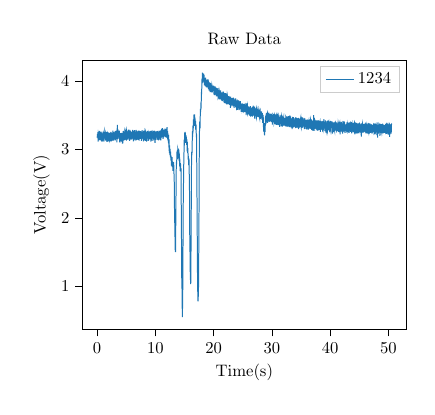
\begin{tikzpicture}[scale=0.6]

    \definecolor{darkgray176}{RGB}{176,176,176}
    \definecolor{lightgray204}{RGB}{204,204,204}
    \definecolor{steelblue31119180}{RGB}{31,119,180}

    \begin{axis}[
            legend cell align={left},
            legend style={fill opacity=0.8, draw opacity=1, text opacity=1, draw=lightgray204},
            tick align=outside,
            tick pos=left,
            title={Raw Data},
            x grid style={darkgray176},
            xlabel={Time(s)},
            xmin=-2.50165, xmax=53.06265,
            xtick style={color=black},
            y grid style={darkgray176},
            ylabel={Voltage(V)},
            ymin=0.373900293255132, ymax=4.29863147605083,
            ytick style={color=black}
        ]
        \addplot [semithick, steelblue31119180]
        table {%
                0.024 3.17204301075269
                0.063 3.2258064516129
                0.095 3.19159335288368
                0.128 3.17693059628543
                0.16 3.25024437927664
                0.192 3.11339198435973
                0.225 3.22091886608016
                0.258 3.20625610948192
                0.29 3.13294232649071
                0.323 3.25024437927664
                0.356 3.19159335288368
                0.388 3.14271749755621
                0.42 3.26979472140762
                0.453 3.13782991202346
                0.485 3.19159335288368
                0.518 3.24046920821114
                0.55 3.13294232649071
                0.583 3.24046920821114
                0.615 3.22091886608016
                0.648 3.13294232649071
                0.679 3.26001955034213
                0.712 3.16226783968719
                0.745 3.16715542521994
                0.777 3.24535679374389
                0.809 3.11339198435973
                0.842 3.2258064516129
                0.874 3.2258064516129
                0.907 3.11827956989247
                0.939 3.2258064516129
                0.971 3.15738025415445
                1.004 3.17693059628543
                1.036 3.26001955034213
                1.069 3.12805474095797
                1.101 3.23069403714565
                1.133 3.24046920821114
                1.166 3.11339198435973
                1.199 3.25024437927664
                1.231 3.26490713587488
                1.263 3.17693059628543
                1.297 3.25024437927664
                1.329 3.17204301075269
                1.361 3.16715542521994
                1.394 3.24046920821114
                1.426 3.13294232649071
                1.459 3.24046920821114
                1.491 3.23069403714565
                1.523 3.12805474095797
                1.556 3.25513196480938
                1.589 3.17693059628543
                1.62 3.15738025415445
                1.653 3.25513196480938
                1.686 3.10850439882698
                1.718 3.21603128054741
                1.751 3.2258064516129
                1.783 3.11339198435973
                1.818 3.2258064516129
                1.851 3.25024437927664
                1.884 3.12316715542522
                1.915 3.24535679374389
                1.948 3.19159335288368
                1.981 3.11827956989247
                2.014 3.2258064516129
                2.046 3.17204301075269
                2.078 3.15738025415445
                2.111 3.24046920821114
                2.144 3.1524926686217
                2.177 3.19159335288368
                2.209 3.23069403714565
                2.241 3.11827956989247
                2.275 3.2258064516129
                2.308 3.24535679374389
                2.34 3.11827956989247
                2.373 3.25513196480938
                2.405 3.17693059628543
                2.438 3.11827956989247
                2.47 3.24535679374389
                2.503 3.14760508308895
                2.536 3.20136852394917
                2.568 3.23069403714565
                2.6 3.14271749755621
                2.633 3.21603128054741
                2.666 3.21114369501466
                2.699 3.12316715542522
                2.731 3.27468230694037
                2.763 3.18670576735093
                2.796 3.13294232649071
                2.829 3.24046920821114
                2.862 3.14760508308895
                2.893 3.20136852394917
                2.926 3.25024437927664
                2.959 3.14760508308895
                2.992 3.24046920821114
                3.024 3.2355816226784
                3.057 3.13294232649071
                3.089 3.24046920821114
                3.122 3.21114369501466
                3.154 3.13294232649071
                3.187 3.26490713587488
                3.22 3.1524926686217
                3.252 3.19159335288368
                3.286 3.27468230694037
                3.318 3.1524926686217
                3.351 3.2355816226784
                3.384 3.2355816226784
                3.416 3.10361681329423
                3.448 3.25024437927664
                3.484 3.35777126099707
                3.516 3.19648093841642
                3.549 3.29912023460411
                3.581 3.25024437927664
                3.614 3.1524926686217
                3.647 3.26001955034213
                3.679 3.22091886608016
                3.712 3.17204301075269
                3.744 3.27468230694037
                3.777 3.17204301075269
                3.81 3.21114369501466
                3.842 3.27468230694037
                3.874 3.10361681329423
                3.907 3.24046920821114
                3.94 3.22091886608016
                3.973 3.10361681329423
                4.004 3.2355816226784
                4.037 3.19159335288368
                4.07 3.13782991202346
                4.103 3.21603128054741
                4.135 3.12316715542522
                4.168 3.19159335288368
                4.2 3.24046920821114
                4.233 3.11339198435973
                4.265 3.21114369501466
                4.299 3.2355816226784
                4.331 3.08406647116325
                4.364 3.20136852394917
                4.397 3.19648093841642
                4.429 3.08895405669599
                4.462 3.26490713587488
                4.494 3.14760508308895
                4.527 3.16715542521994
                4.559 3.2355816226784
                4.592 3.12805474095797
                4.625 3.24046920821114
                4.658 3.25513196480938
                4.689 3.13782991202346
                4.722 3.25513196480938
                4.755 3.2355816226784
                4.788 3.13782991202346
                4.82 3.26001955034213
                4.852 3.20136852394917
                4.885 3.17204301075269
                4.918 3.28445747800587
                4.951 3.14271749755621
                4.983 3.26001955034213
                5.015 3.25024437927664
                5.048 3.12805474095797
                5.081 3.26490713587488
                5.113 3.25024437927664
                5.148 3.1524926686217
                5.181 3.25513196480938
                5.214 3.25024437927664
                5.246 3.14271749755621
                5.279 3.26001955034213
                5.312 3.2355816226784
                5.345 3.1524926686217
                5.378 3.28934506353861
                5.41 3.18181818181818
                5.442 3.19159335288368
                5.475 3.26979472140762
                5.508 3.16226783968719
                5.54 3.26001955034213
                5.572 3.26490713587488
                5.605 3.12316715542522
                5.638 3.28445747800587
                5.67 3.2258064516129
                5.703 3.14760508308895
                5.736 3.26979472140762
                5.768 3.20625610948192
                5.8 3.18670576735093
                5.833 3.26001955034213
                5.866 3.14271749755621
                5.898 3.23069403714565
                5.931 3.25024437927664
                5.963 3.14760508308895
                5.996 3.26001955034213
                6.029 3.20625610948192
                6.061 3.15738025415445
                6.093 3.28445747800587
                6.126 3.17204301075269
                6.159 3.21603128054741
                6.192 3.27468230694037
                6.224 3.11827956989247
                6.256 3.25024437927664
                6.29 3.26979472140762
                6.323 3.12805474095797
                6.355 3.24046920821114
                6.388 3.2355816226784
                6.42 3.14271749755621
                6.453 3.27956989247312
                6.486 3.19159335288368
                6.518 3.18181818181818
                6.55 3.24046920821114
                6.583 3.16226783968719
                6.616 3.18670576735093
                6.648 3.26001955034213
                6.681 3.12805474095797
                6.714 3.28445747800587
                6.746 3.24046920821114
                6.778 3.17204301075269
                6.811 3.26979472140762
                6.846 3.22091886608016
                6.879 3.13782991202346
                6.912 3.25024437927664
                6.944 3.14760508308895
                6.976 3.17693059628543
                7.009 3.26001955034213
                7.042 3.16226783968719
                7.074 3.21114369501466
                7.107 3.27468230694037
                7.139 3.13782991202346
                7.172 3.24535679374389
                7.204 3.25024437927664
                7.237 3.12805474095797
                7.27 3.26979472140762
                7.303 3.2258064516129
                7.335 3.1524926686217
                7.368 3.26001955034213
                7.401 3.18670576735093
                7.434 3.18670576735093
                7.465 3.26490713587488
                7.498 3.1524926686217
                7.531 3.23069403714565
                7.564 3.2355816226784
                7.596 3.12316715542522
                7.628 3.24535679374389
                7.661 3.21603128054741
                7.694 3.14760508308895
                7.727 3.27956989247312
                7.758 3.17204301075269
                7.791 3.19648093841642
                7.824 3.26001955034213
                7.857 3.15738025415445
                7.889 3.22091886608016
                7.921 3.25024437927664
                7.954 3.11827956989247
                7.987 3.26979472140762
                8.019 3.21114369501466
                8.052 3.13782991202346
                8.084 3.27468230694037
                8.117 3.17204301075269
                8.15 3.20625610948192
                8.182 3.26979472140762
                8.215 3.12805474095797
                8.247 3.24535679374389
                8.28 3.23069403714565
                8.313 3.12316715542522
                8.346 3.24046920821114
                8.379 3.2258064516129
                8.411 3.14760508308895
                8.443 3.26001955034213
                8.476 3.20625610948192
                8.511 3.11339198435973
                8.544 3.26001955034213
                8.577 3.20136852394917
                8.609 3.16715542521994
                8.641 3.26979472140762
                8.674 3.15738025415445
                8.707 3.20625610948192
                8.739 3.26001955034213
                8.772 3.12316715542522
                8.805 3.23069403714565
                8.837 3.24046920821114
                8.869 3.12805474095797
                8.902 3.26001955034213
                8.935 3.20136852394917
                8.968 3.15738025415445
                8.999 3.26001955034213
                9.032 3.17204301075269
                9.065 3.20625610948192
                9.098 3.26490713587488
                9.131 3.14760508308895
                9.162 3.24046920821114
                9.195 3.2355816226784
                9.228 3.11339198435973
                9.261 3.27468230694037
                9.294 3.2258064516129
                9.327 3.12805474095797
                9.36 3.26979472140762
                9.392 3.21114369501466
                9.424 3.17693059628543
                9.457 3.26001955034213
                9.49 3.15738025415445
                9.522 3.24535679374389
                9.554 3.25024437927664
                9.587 3.12316715542522
                9.62 3.2355816226784
                9.653 3.2258064516129
                9.686 3.14271749755621
                9.717 3.26490713587488
                9.75 3.19648093841642
                9.783 3.14271749755621
                9.816 3.26979472140762
                9.848 3.14760508308895
                9.881 3.23069403714565
                9.913 3.26979472140762
                9.946 3.09384164222874
                9.978 3.23069403714565
                10.011 3.22091886608016
                10.044 3.13782991202346
                10.076 3.26001955034213
                10.108 3.20625610948192
                10.141 3.14271749755621
                10.177 3.25024437927664
                10.209 3.2258064516129
                10.242 3.17693059628543
                10.274 3.26490713587488
                10.308 3.19648093841642
                10.341 3.17204301075269
                10.374 3.25024437927664
                10.405 3.14271749755621
                10.438 3.17204301075269
                10.471 3.26490713587488
                10.504 3.13294232649071
                10.536 3.25024437927664
                10.569 3.24535679374389
                10.601 3.13782991202346
                10.634 3.24535679374389
                10.667 3.20136852394917
                10.699 3.15738025415445
                10.732 3.26979472140762
                10.765 3.16226783968719
                10.797 3.19159335288368
                10.829 3.27468230694037
                10.862 3.13294232649071
                10.895 3.24535679374389
                10.928 3.25024437927664
                10.96 3.13294232649071
                10.993 3.28445747800587
                11.025 3.24046920821114
                11.058 3.17204301075269
                11.09 3.29423264907136
                11.123 3.20136852394917
                11.156 3.23069403714565
                11.189 3.3088954056696
                11.22 3.18181818181818
                11.253 3.26490713587488
                11.286 3.29423264907136
                11.32 3.1524926686217
                11.353 3.26490713587488
                11.385 3.25513196480938
                11.417 3.17693059628543
                11.45 3.28445747800587
                11.483 3.22091886608016
                11.515 3.18670576735093
                11.548 3.27468230694037
                11.581 3.19159335288368
                11.613 3.2355816226784
                11.645 3.30400782013685
                11.681 3.23069403714565
                11.713 3.2258064516129
                11.746 3.29912023460411
                11.779 3.18181818181818
                11.81 3.27468230694037
                11.843 3.29423264907136
                11.876 3.17204301075269
                11.909 3.29912023460411
                11.94 3.2355816226784
                11.973 3.22091886608016
                12.006 3.32355816226784
                12.038 3.20625610948192
                12.07 3.26001955034213
                12.103 3.26001955034213
                12.135 3.14271749755621
                12.168 3.2355816226784
                12.2 3.15738025415445
                12.233 3.09872922776149
                12.265 3.21114369501466
                12.299 3.09872922776149
                12.332 3.03030303030303
                12.363 3.14760508308895
                12.396 2.94721407624633
                12.429 3.02541544477028
                12.462 3.05962854349951
                12.493 2.91788856304985
                12.526 3.0058651026393
                12.559 2.95698924731183
                12.591 2.88367546432063
                12.623 2.96676441837732
                12.656 2.86412512218964
                12.688 2.86901270772239
                12.721 2.90811339198436
                12.753 2.76148582600196
                12.786 2.86412512218964
                12.818 2.81036168132942
                12.851 2.75171065493646
                12.883 2.88856304985337
                12.915 2.78103616813294
                12.948 2.74193548387097
                12.981 2.82502443792766
                13.014 2.68817204301075
                13.045 2.79569892473118
                13.078 2.81524926686217
                13.111 2.6930596285435
                13.143 2.81036168132942
                13.175 2.74682306940371
                13.21 2.62952101661779
                13.243 2.57575757575758
                13.276 2.31182795698925
                13.308 1.95503421309873
                13.341 1.95992179863148
                13.374 1.74486803519062
                13.407 1.544477028348
                13.438 1.52492668621701
                13.471 1.50048875855327
                13.504 1.85728250244379
                13.537 2.2238514173998
                13.569 2.47311827956989
                13.601 2.80058651026393
                13.634 2.81524926686217
                13.666 2.78103616813294
                13.699 2.96676441837732
                13.731 2.85923753665689
                13.763 2.94232649071359
                13.796 2.99120234604106
                13.829 2.85923753665689
                13.861 3.00097751710655
                13.893 2.98631476050831
                13.926 2.87390029325513
                13.959 3.01075268817204
                13.99 2.93743890518084
                14.023 2.90322580645161
                14.056 2.9960899315738
                14.089 2.82991202346041
                14.12 2.93255131964809
                14.153 2.87878787878788
                14.186 2.75171065493646
                14.218 2.85434995112414
                14.251 2.73704789833822
                14.283 2.67839687194526
                14.316 2.80058651026393
                14.349 2.70772238514174
                14.382 2.70283479960899
                14.414 2.72238514173998
                14.446 2.23851417399804
                14.479 1.88172043010753
                14.512 1.44672531769306
                14.543 1.02150537634409
                14.576 0.987292277614858
                14.609 0.752688172043011
                14.642 0.552297165200391
                14.673 0.718475073313783
                14.709 0.957966764418377
                14.742 1.41251221896383
                14.774 2.05767350928641
                14.807 2.33137829912023
                14.839 2.52199413489736
                14.872 2.77126099706745
                14.905 2.81524926686217
                14.938 3.08895405669599
                14.969 3.14760508308895
                15.002 3.05962854349951
                15.035 3.24535679374389
                15.068 3.19159335288368
                15.1 3.12316715542522
                15.133 3.25513196480938
                15.165 3.13294232649071
                15.198 3.16715542521994
                15.23 3.20625610948192
                15.263 3.09384164222874
                15.296 3.19648093841642
                15.33 3.1524926686217
                15.362 3.06451612903226
                15.394 3.14760508308895
                15.427 3.11827956989247
                15.46 2.97165200391007
                15.493 3.10850439882698
                15.525 3.00097751710655
                15.558 2.94721407624633
                15.591 3.02052785923754
                15.623 2.87878787878788
                15.655 2.8494623655914
                15.688 2.90322580645161
                15.721 2.77126099706745
                15.754 2.80547409579668
                15.787 2.81524926686217
                15.818 2.64418377321603
                15.851 2.6099706744868
                15.884 2.14076246334311
                15.917 1.62267839687195
                15.949 1.52492668621701
                15.982 1.27077223851417
                16.015 1.11436950146628
                16.048 1.08993157380254
                16.079 1.03616813294233
                16.112 1.32942326490714
                16.145 1.83773216031281
                16.178 2.27272727272727
                16.21 2.7761485826002
                16.246 2.96187683284457
                16.278 2.91788856304985
                16.316 2.98631476050831
                16.349 3.19648093841642
                16.381 3.26490713587488
                16.414 3.18181818181818
                16.447 3.34799608993157
                16.48 3.26490713587488
                16.513 3.31378299120235
                16.544 3.43597262952102
                16.577 3.34310850439883
                16.61 3.46041055718475
                16.643 3.50928641251222
                16.675 3.35777126099707
                16.708 3.47996089931574
                16.741 3.48484848484848
                16.774 3.33822091886608
                16.805 3.4652981427175
                16.838 3.36265884652981
                16.871 3.35777126099707
                16.904 3.41642228739003
                16.936 3.28934506353861
                16.969 3.33822091886608
                17.002 3.36265884652981
                17.035 3.17693059628543
                17.067 3.2258064516129
                17.099 2.95210166177908
                17.132 2.52688172043011
                17.165 2.16520039100684
                17.198 1.71065493646139
                17.23 1.24633431085044
                17.263 1.07038123167155
                17.296 0.811339198435973
                17.329 0.782013685239492
                17.361 0.879765395894428
                17.394 0.850439882697947
                17.427 1.11436950146628
                17.46 1.57869012707722
                17.492 1.98924731182796
                17.524 2.63440860215054
                17.557 3.16226783968719
                17.59 3.29912023460411
                17.623 3.40664711632454
                17.655 3.33822091886608
                17.688 3.33333333333333
                17.721 3.54838709677419
                17.756 3.59237536656891
                17.788 3.54349951124145
                17.821 3.68035190615836
                17.853 3.59726295210166
                17.886 3.71456500488759
                17.918 3.83675464320626
                17.951 3.80254154447703
                17.984 3.95894428152493
                18.017 4.03714565004888
                18.049 3.96383186705767
                18.081 4.12023460410557
                18.114 4.07624633431085
                18.147 3.97360703812317
                18.18 4.11045943304008
                18.212 4.01759530791789
                18.244 4.02248289345064
                18.277 4.10557184750733
                18.31 3.98826979472141
                18.343 4.02737047898338
                18.376 4.08602150537634
                18.409 3.93450635386119
                18.441 4.02737047898338
                18.473 4.01759530791789
                18.506 3.93450635386119
                18.539 4.04203323558162
                18.572 3.98338220918866
                18.605 3.91984359726295
                18.636 4.04692082111437
                18.669 3.92961876832845
                18.702 3.97360703812317
                18.735 4.01759530791789
                18.767 3.90518084066471
                18.8 4.01759530791789
                18.832 3.99315738025415
                18.865 3.91006842619746
                18.897 3.98826979472141
                18.93 3.93939393939394
                18.963 3.98338220918866
                18.995 4.02248289345064
                19.027 3.90029325513196
                19.06 3.93939393939394
                19.093 3.98826979472141
                19.126 3.88074291300098
                19.159 3.97849462365591
                19.19 3.96871945259042
                19.223 3.85630498533724
                19.256 3.97849462365591
                19.291 3.94428152492669
                19.324 3.87585532746823
                19.357 3.95894428152493
                19.39 3.93939393939394
                19.423 3.83675464320626
                19.456 3.96871945259042
                19.487 3.91006842619746
                19.52 3.86119257086999
                19.553 3.94428152492669
                19.586 3.83675464320626
                19.618 3.90029325513196
                19.65 3.94428152492669
                19.683 3.83186705767351
                19.716 3.93450635386119
                19.748 3.91984359726295
                19.781 3.83186705767351
                19.814 3.92961876832845
                19.846 3.88074291300098
                19.878 3.85630498533724
                19.911 3.91495601173021
                19.944 3.87585532746823
                19.977 3.88074291300098
                20.008 3.92961876832845
                20.041 3.80254154447703
                20.074 3.89051808406647
                20.107 3.89540566959922
                20.14 3.79276637341153
                20.172 3.90518084066471
                20.205 3.86119257086999
                20.237 3.81231671554252
                20.27 3.91984359726295
                20.302 3.81231671554252
                20.336 3.81720430107527
                20.369 3.90518084066471
                20.401 3.79765395894428
                20.433 3.86608015640274
                20.466 3.87096774193548
                20.499 3.77321603128055
                20.532 3.88074291300098
                20.564 3.84652981427175
                20.596 3.77321603128055
                20.629 3.88563049853372
                20.662 3.80254154447703
                20.695 3.82209188660802
                20.727 3.89540566959922
                20.76 3.75855327468231
                20.795 3.7683284457478
                20.828 3.86608015640274
                20.86 3.77810361681329
                20.892 3.80742913000978
                20.925 3.86119257086999
                20.958 3.72922776148583
                20.99 3.84652981427175
                21.023 3.83186705767351
                21.056 3.72922776148583
                21.088 3.841642228739
                21.121 3.80742913000978
                21.153 3.76344086021505
                21.186 3.86119257086999
                21.219 3.7683284457478
                21.252 3.80742913000978
                21.284 3.83186705767351
                21.316 3.72434017595308
                21.35 3.80254154447703
                21.383 3.83186705767351
                21.415 3.70967741935484
                21.448 3.83186705767351
                21.481 3.79276637341153
                21.513 3.70478983382209
                21.545 3.81720430107527
                21.578 3.77321603128055
                21.611 3.72922776148583
                21.644 3.84652981427175
                21.677 3.71945259042033
                21.708 3.7683284457478
                21.741 3.82697947214076
                21.774 3.69012707722385
                21.807 3.81231671554252
                21.839 3.80742913000978
                21.872 3.67546432062561
                21.904 3.79765395894428
                21.937 3.73900293255132
                21.969 3.73900293255132
                22.002 3.82209188660802
                22.035 3.6950146627566
                22.068 3.74877810361681
                22.099 3.81231671554252
                22.132 3.66568914956012
                22.165 3.77321603128055
                22.198 3.7683284457478
                22.231 3.65591397849462
                22.263 3.81720430107527
                22.296 3.72434017595308
                22.332 3.65591397849462
                22.365 3.78787878787879
                22.397 3.77321603128055
                22.43 3.66080156402737
                22.462 3.77321603128055
                22.495 3.70478983382209
                22.528 3.67546432062561
                22.56 3.77810361681329
                22.593 3.6852394916911
                22.626 3.69012707722385
                22.658 3.7683284457478
                22.69 3.65102639296188
                22.723 3.75855327468231
                22.756 3.75366568914956
                22.789 3.65102639296188
                22.821 3.74877810361681
                22.854 3.72434017595308
                22.887 3.60703812316716
                22.919 3.7683284457478
                22.951 3.6950146627566
                22.984 3.6852394916911
                23.017 3.74877810361681
                23.05 3.67546432062561
                23.083 3.72434017595308
                23.114 3.72922776148583
                23.147 3.62658846529814
                23.18 3.72434017595308
                23.213 3.74877810361681
                23.245 3.64613880742913
                23.278 3.74389051808407
                23.31 3.66568914956012
                23.344 3.64613880742913
                23.376 3.75366568914956
                23.409 3.63636363636364
                23.442 3.69012707722385
                23.475 3.71945259042033
                23.506 3.60703812316716
                23.539 3.70967741935484
                23.572 3.69990224828934
                23.605 3.63147605083089
                23.638 3.72434017595308
                23.67 3.67057673509286
                23.703 3.63636363636364
                23.735 3.74389051808407
                23.768 3.6217008797654
                23.8 3.67057673509286
                23.833 3.73900293255132
                23.864 3.60703812316716
                23.896 3.70967741935484
                23.928 3.62658846529814
                23.961 3.64125122189638
                23.993 3.71456500488759
                24.026 3.57771260997067
                24.058 3.69990224828934
                24.09 3.70478983382209
                24.123 3.57771260997067
                24.156 3.69990224828934
                24.188 3.63636363636364
                24.22 3.59726295210166
                24.253 3.71456500488759
                24.286 3.60215053763441
                24.318 3.64613880742913
                24.351 3.69012707722385
                24.384 3.57282502443793
                24.417 3.69012707722385
                24.449 3.6852394916911
                24.481 3.58260019550342
                24.514 3.69990224828934
                24.546 3.6217008797654
                24.579 3.58748778103617
                24.611 3.70478983382209
                24.644 3.58748778103617
                24.676 3.64125122189638
                24.709 3.66568914956012
                24.741 3.54838709677419
                24.773 3.66568914956012
                24.806 3.6217008797654
                24.839 3.56793743890518
                24.871 3.65102639296188
                24.903 3.58260019550342
                24.936 3.59726295210166
                24.969 3.66080156402737
                25 3.54838709677419
                25.033 3.65102639296188
                25.066 3.64613880742913
                25.099 3.54349951124145
                25.131 3.66568914956012
                25.163 3.57282502443793
                25.196 3.58260019550342
                25.228 3.65102639296188
                25.261 3.54349951124145
                25.293 3.63147605083089
                25.326 3.64613880742913
                25.369 3.63636363636364
                25.404 3.6217008797654
                25.439 3.54349951124145
                25.474 3.59237536656891
                25.508 3.62658846529814
                25.542 3.6119257086999
                25.577 3.49951124144673
                25.612 3.60703812316716
                25.647 3.67057673509286
                25.681 3.57771260997067
                25.715 3.52883675464321
                25.75 3.62658846529814
                25.785 3.64125122189638
                25.82 3.51906158357771
                25.854 3.52883675464321
                25.889 3.6217008797654
                25.924 3.6217008797654
                25.958 3.51417399804497
                25.993 3.54349951124145
                26.028 3.62658846529814
                26.062 3.58748778103617
                26.097 3.49951124144673
                26.131 3.54838709677419
                26.166 3.6119257086999
                26.201 3.58260019550342
                26.235 3.48973607038123
                26.27 3.56793743890518
                26.304 3.63147605083089
                26.339 3.55816226783969
                26.374 3.47996089931574
                26.409 3.56304985337243
                26.444 3.60215053763441
                26.478 3.55327468230694
                26.513 3.48973607038123
                26.548 3.56304985337243
                26.583 3.6119257086999
                26.617 3.52394916911046
                26.651 3.47996089931574
                26.686 3.60215053763441
                26.721 3.59726295210166
                26.756 3.54349951124145
                26.79 3.49951124144673
                26.824 3.59726295210166
                26.859 3.58748778103617
                26.894 3.50928641251222
                26.929 3.48973607038123
                26.963 3.61681329423265
                27 3.6119257086999
                27.035 3.52394916911046
                27.07 3.44574780058651
                27.105 3.54349951124145
                27.14 3.59726295210166
                27.174 3.49462365591398
                27.209 3.53372434017595
                27.244 3.57282502443793
                27.279 3.58748778103617
                27.314 3.48973607038123
                27.347 3.47507331378299
                27.382 3.58260019550342
                27.417 3.59237536656891
                27.453 3.50928641251222
                27.488 3.47996089931574
                27.523 3.56793743890518
                27.557 3.57282502443793
                27.592 3.50439882697947
                27.627 3.47018572825024
                27.662 3.55816226783969
                27.697 3.56304985337243
                27.731 3.47996089931574
                27.766 3.47996089931574
                27.8 3.57282502443793
                27.835 3.55816226783969
                27.87 3.47018572825024
                27.905 3.455522971652
                27.939 3.55327468230694
                27.974 3.56304985337243
                28.009 3.44574780058651
                28.044 3.4652981427175
                28.079 3.54838709677419
                28.113 3.52883675464321
                28.148 3.455522971652
                28.183 3.47996089931574
                28.218 3.55327468230694
                28.253 3.51906158357771
                28.288 3.43597262952102
                28.322 3.47996089931574
                28.357 3.52883675464321
                28.392 3.49951124144673
                28.427 3.38709677419355
                28.461 3.47996089931574
                28.495 3.50439882697947
                28.531 3.455522971652
                28.566 3.31867057673509
                28.604 3.26001955034213
                28.639 3.3822091886608
                28.674 3.36265884652981
                28.708 3.26490713587488
                28.742 3.20625610948192
                28.777 3.3088954056696
                28.812 3.33333333333333
                28.847 3.31867057673509
                28.881 3.43597262952102
                28.916 3.47507331378299
                28.951 3.48484848484848
                28.986 3.3822091886608
                29.021 3.3919843597263
                29.056 3.53372434017595
                29.09 3.47507331378299
                29.125 3.41153470185728
                29.16 3.41642228739003
                29.195 3.51906158357771
                29.23 3.52883675464321
                29.264 3.38709677419355
                29.299 3.43597262952102
                29.334 3.51417399804497
                29.369 3.49951124144673
                29.403 3.41153470185728
                29.437 3.43597262952102
                29.472 3.53372434017595
                29.507 3.51417399804497
                29.542 3.40175953079179
                29.577 3.44574780058651
                29.613 3.51906158357771
                29.647 3.48973607038123
                29.682 3.40664711632454
                29.717 3.43597262952102
                29.752 3.49951124144673
                29.787 3.50439882697947
                29.821 3.41153470185728
                29.856 3.43108504398827
                29.891 3.51906158357771
                29.925 3.48484848484848
                29.96 3.39687194525904
                29.995 3.46041055718475
                30.029 3.49951124144673
                30.064 3.47507331378299
                30.099 3.36265884652981
                30.134 3.45063538611926
                30.169 3.49951124144673
                30.203 3.48973607038123
                30.241 3.42130987292278
                30.275 3.39687194525904
                30.31 3.50928641251222
                30.345 3.50928641251222
                30.38 3.3919843597263
                30.414 3.40664711632454
                30.449 3.50439882697947
                30.484 3.49462365591398
                30.519 3.36754643206256
                30.554 3.3919843597263
                30.588 3.50928641251222
                30.623 3.47018572825024
                30.658 3.40175953079179
                30.693 3.41153470185728
                30.728 3.50928641251222
                30.763 3.47018572825024
                30.797 3.35777126099707
                30.832 3.38709677419355
                30.867 3.48484848484848
                30.902 3.47018572825024
                30.937 3.36265884652981
                30.971 3.39687194525904
                31.006 3.47996089931574
                31.041 3.4652981427175
                31.076 3.35288367546432
                31.111 3.41642228739003
                31.144 3.47018572825024
                31.179 3.45063538611926
                31.214 3.35288367546432
                31.249 3.41153470185728
                31.284 3.47507331378299
                31.319 3.42619745845552
                31.353 3.32844574780059
                31.388 3.47018572825024
                31.423 3.50439882697947
                31.458 3.41642228739003
                31.493 3.36754643206256
                31.527 3.43597262952102
                31.562 3.47996089931574
                31.597 3.40664711632454
                31.631 3.34310850439883
                31.666 3.47996089931574
                31.7 3.4652981427175
                31.736 3.42130987292278
                31.771 3.32844574780059
                31.806 3.43108504398827
                31.843 3.4652981427175
                31.878 3.455522971652
                31.912 3.36754643206256
                31.947 3.34310850439883
                31.982 3.45063538611926
                32.017 3.4652981427175
                32.052 3.35288367546432
                32.087 3.3919843597263
                32.121 3.46041055718475
                32.156 3.43597262952102
                32.191 3.34799608993157
                32.226 3.3919843597263
                32.261 3.46041055718475
                32.294 3.44086021505376
                32.329 3.33822091886608
                32.364 3.41153470185728
                32.399 3.47018572825024
                32.434 3.46041055718475
                32.468 3.33333333333333
                32.503 3.40664711632454
                32.538 3.47996089931574
                32.573 3.3919843597263
                32.608 3.33822091886608
                32.643 3.41642228739003
                32.677 3.47507331378299
                32.712 3.39687194525904
                32.747 3.32844574780059
                32.782 3.455522971652
                32.817 3.48484848484848
                32.851 3.40664711632454
                32.886 3.34310850439883
                32.921 3.44574780058651
                32.956 3.48484848484848
                32.991 3.39687194525904
                33.026 3.32355816226784
                33.06 3.42619745845552
                33.095 3.49462365591398
                33.13 3.39687194525904
                33.165 3.33333333333333
                33.2 3.44574780058651
                33.234 3.47996089931574
                33.269 3.37243401759531
                33.304 3.31867057673509
                33.339 3.41642228739003
                33.378 3.44574780058651
                33.413 3.44574780058651
                33.447 3.36265884652981
                33.485 3.29423264907136
                33.519 3.40175953079179
                33.554 3.47507331378299
                33.589 3.40175953079179
                33.624 3.31378299120235
                33.658 3.40175953079179
                33.693 3.47018572825024
                33.729 3.41153470185728
                33.764 3.32844574780059
                33.798 3.40175953079179
                33.832 3.41642228739003
                33.868 3.41153470185728
                33.903 3.33333333333333
                33.938 3.40175953079179
                33.973 3.46041055718475
                34.008 3.41642228739003
                34.042 3.3088954056696
                34.077 3.37732160312805
                34.112 3.47018572825024
                34.147 3.40664711632454
                34.182 3.31378299120235
                34.216 3.36754643206256
                34.251 3.455522971652
                34.286 3.3919843597263
                34.321 3.32355816226784
                34.356 3.41153470185728
                34.391 3.45063538611926
                34.425 3.40664711632454
                34.46 3.3088954056696
                34.495 3.38709677419355
                34.53 3.46041055718475
                34.565 3.3919843597263
                34.598 3.29423264907136
                34.633 3.38709677419355
                34.668 3.44574780058651
                34.703 3.38709677419355
                34.738 3.31867057673509
                34.772 3.39687194525904
                34.807 3.45063538611926
                34.842 3.3822091886608
                34.877 3.32844574780059
                34.912 3.44574780058651
                34.948 3.46041055718475
                34.982 3.33822091886608
                35.017 3.32355816226784
                35.051 3.42130987292278
                35.089 3.44086021505376
                35.124 3.42619745845552
                35.159 3.31378299120235
                35.193 3.36754643206256
                35.228 3.4652981427175
                35.263 3.39687194525904
                35.298 3.31867057673509
                35.333 3.38709677419355
                35.367 3.43597262952102
                35.402 3.39687194525904
                35.437 3.33822091886608
                35.471 3.36754643206256
                35.506 3.46041055718475
                35.54 3.41642228739003
                35.575 3.29423264907136
                35.61 3.3822091886608
                35.645 3.45063538611926
                35.68 3.40175953079179
                35.715 3.32355816226784
                35.749 3.39687194525904
                35.784 3.43108504398827
                35.819 3.37243401759531
                35.854 3.29912023460411
                35.889 3.39687194525904
                35.923 3.42619745845552
                35.958 3.35288367546432
                35.993 3.28934506353861
                36.028 3.3822091886608
                36.063 3.43597262952102
                36.098 3.37243401759531
                36.132 3.30400782013685
                36.167 3.39687194525904
                36.202 3.43108504398827
                36.237 3.3822091886608
                36.272 3.28934506353861
                36.306 3.40175953079179
                36.341 3.41642228739003
                36.376 3.36754643206256
                36.411 3.3088954056696
                36.446 3.40175953079179
                36.481 3.43597262952102
                36.515 3.33822091886608
                36.55 3.29912023460411
                36.585 3.41642228739003
                36.62 3.43108504398827
                36.655 3.33333333333333
                36.688 3.30400782013685
                36.726 3.34310850439883
                36.761 3.43597262952102
                36.795 3.3822091886608
                36.83 3.28445747800587
                36.865 3.37243401759531
                36.899 3.42130987292278
                36.934 3.37243401759531
                36.969 3.27468230694037
                37.003 3.3919843597263
                37.038 3.41642228739003
                37.073 3.33333333333333
                37.108 3.27468230694037
                37.142 3.40664711632454
                37.177 3.49951124144673
                37.212 3.36754643206256
                37.246 3.26979472140762
                37.281 3.41153470185728
                37.315 3.42130987292278
                37.35 3.32355816226784
                37.385 3.29912023460411
                37.42 3.41153470185728
                37.454 3.40175953079179
                37.489 3.30400782013685
                37.523 3.32844574780059
                37.558 3.42130987292278
                37.593 3.39687194525904
                37.627 3.33333333333333
                37.662 3.34799608993157
                37.697 3.42130987292278
                37.731 3.36265884652981
                37.766 3.27956989247312
                37.8 3.36754643206256
                37.835 3.42130987292278
                37.87 3.34310850439883
                37.904 3.26979472140762
                37.939 3.40175953079179
                37.974 3.3822091886608
                38.008 3.33822091886608
                38.043 3.28445747800587
                38.077 3.40175953079179
                38.112 3.39687194525904
                38.148 3.31867057673509
                38.182 3.28445747800587
                38.216 3.40175953079179
                38.251 3.41153470185728
                38.286 3.30400782013685
                38.323 3.25513196480938
                38.358 3.37732160312805
                38.392 3.41642228739003
                38.427 3.33822091886608
                38.462 3.28445747800587
                38.496 3.3822091886608
                38.531 3.40664711632454
                38.565 3.29912023460411
                38.6 3.29912023460411
                38.635 3.38709677419355
                38.669 3.40664711632454
                38.704 3.31867057673509
                38.738 3.25513196480938
                38.773 3.41642228739003
                38.808 3.3822091886608
                38.843 3.29423264907136
                38.877 3.3088954056696
                38.912 3.44086021505376
                38.946 3.37732160312805
                38.981 3.30400782013685
                39.016 3.35288367546432
                39.05 3.40175953079179
                39.085 3.35288367546432
                39.119 3.26490713587488
                39.154 3.37732160312805
                39.189 3.42130987292278
                39.224 3.37243401759531
                39.259 3.24535679374389
                39.293 3.37732160312805
                39.328 3.41153470185728
                39.363 3.27956989247312
                39.397 3.26490713587488
                39.432 3.38709677419355
                39.467 3.38709677419355
                39.501 3.29912023460411
                39.536 3.28445747800587
                39.57 3.41153470185728
                39.605 3.41153470185728
                39.64 3.27956989247312
                39.674 3.29912023460411
                39.709 3.38709677419355
                39.744 3.39687194525904
                39.778 3.27956989247312
                39.813 3.32355816226784
                39.847 3.40175953079179
                39.882 3.34799608993157
                39.917 3.26979472140762
                39.954 3.27468230694037
                39.989 3.36754643206256
                40.024 3.41642228739003
                40.058 3.28934506353861
                40.093 3.27468230694037
                40.128 3.3919843597263
                40.163 3.38709677419355
                40.198 3.3088954056696
                40.232 3.36265884652981
                40.267 3.3919843597263
                40.302 3.41153470185728
                40.337 3.29912023460411
                40.372 3.23069403714565
                40.407 3.3822091886608
                40.441 3.37732160312805
                40.476 3.31867057673509
                40.511 3.27956989247312
                40.546 3.38709677419355
                40.581 3.38709677419355
                40.615 3.26979472140762
                40.65 3.27468230694037
                40.685 3.3919843597263
                40.72 3.37243401759531
                40.755 3.27956989247312
                40.79 3.26490713587488
                40.824 3.3919843597263
                40.859 3.39687194525904
                40.894 3.27468230694037
                40.929 3.29912023460411
                40.964 3.38709677419355
                40.998 3.3822091886608
                41.032 3.29423264907136
                41.067 3.28445747800587
                41.102 3.3919843597263
                41.137 3.35777126099707
                41.171 3.26001955034213
                41.206 3.3088954056696
                41.241 3.36265884652981
                41.276 3.36754643206256
                41.311 3.26979472140762
                41.346 3.32355816226784
                41.381 3.3919843597263
                41.416 3.37732160312805
                41.451 3.25513196480938
                41.486 3.31867057673509
                41.521 3.37243401759531
                41.555 3.36754643206256
                41.587 3.25024437927664
                41.622 3.38709677419355
                41.657 3.39687194525904
                41.692 3.33822091886608
                41.726 3.22091886608016
                41.761 3.35288367546432
                41.796 3.3919843597263
                41.831 3.29912023460411
                41.866 3.26001955034213
                41.901 3.37732160312805
                41.935 3.40175953079179
                41.97 3.30400782013685
                42.005 3.26490713587488
                42.04 3.37243401759531
                42.075 3.37243401759531
                42.109 3.25513196480938
                42.144 3.23069403714565
                42.179 3.3919843597263
                42.213 3.38709677419355
                42.248 3.32355816226784
                42.283 3.26001955034213
                42.317 3.36754643206256
                42.352 3.41153470185728
                42.387 3.26490713587488
                42.422 3.26001955034213
                42.458 3.3919843597263
                42.492 3.38709677419355
                42.527 3.29423264907136
                42.562 3.26979472140762
                42.597 3.35777126099707
                42.632 3.33333333333333
                42.667 3.29423264907136
                42.701 3.24046920821114
                42.736 3.36265884652981
                42.771 3.36265884652981
                42.805 3.26001955034213
                42.84 3.28445747800587
                42.874 3.37243401759531
                42.909 3.36754643206256
                42.944 3.26001955034213
                42.979 3.26001955034213
                43.014 3.36754643206256
                43.048 3.35288367546432
                43.083 3.26979472140762
                43.118 3.27956989247312
                43.153 3.3822091886608
                43.191 3.3822091886608
                43.226 3.29912023460411
                43.26 3.24046920821114
                43.294 3.35288367546432
                43.329 3.3919843597263
                43.364 3.31378299120235
                43.399 3.26490713587488
                43.433 3.36265884652981
                43.468 3.37243401759531
                43.504 3.28934506353861
                43.539 3.25513196480938
                43.574 3.33822091886608
                43.609 3.39687194525904
                43.643 3.30400782013685
                43.678 3.2355816226784
                43.713 3.37243401759531
                43.747 3.3822091886608
                43.782 3.31378299120235
                43.816 3.26001955034213
                43.851 3.36265884652981
                43.886 3.38709677419355
                43.921 3.27468230694037
                43.956 3.25024437927664
                43.991 3.35288367546432
                44.025 3.38709677419355
                44.06 3.28445747800587
                44.095 3.25513196480938
                44.13 3.37732160312805
                44.165 3.38709677419355
                44.199 3.26979472140762
                44.234 3.22091886608016
                44.268 3.3919843597263
                44.303 3.37243401759531
                44.338 3.25024437927664
                44.372 3.25513196480938
                44.407 3.37243401759531
                44.442 3.36754643206256
                44.477 3.2355816226784
                44.512 3.30400782013685
                44.547 3.38709677419355
                44.582 3.34310850439883
                44.616 3.23069403714565
                44.651 3.28445747800587
                44.686 3.36265884652981
                44.721 3.35777126099707
                44.755 3.24046920821114
                44.79 3.28445747800587
                44.828 3.34799608993157
                44.863 3.37732160312805
                44.898 3.29423264907136
                44.933 3.2355816226784
                44.966 3.35777126099707
                45.001 3.3822091886608
                45.036 3.28445747800587
                45.071 3.25513196480938
                45.106 3.37243401759531
                45.14 3.36754643206256
                45.175 3.29912023460411
                45.21 3.24535679374389
                45.245 3.35777126099707
                45.28 3.35777126099707
                45.315 3.26490713587488
                45.349 3.18670576735093
                45.384 3.36265884652981
                45.419 3.35777126099707
                45.454 3.25513196480938
                45.489 3.26490713587488
                45.522 3.36265884652981
                45.557 3.37732160312805
                45.592 3.26979472140762
                45.627 3.24535679374389
                45.663 3.33822091886608
                45.698 3.34310850439883
                45.732 3.27468230694037
                45.767 3.25024437927664
                45.802 3.36265884652981
                45.837 3.36265884652981
                45.872 3.26979472140762
                45.905 3.27468230694037
                45.94 3.36265884652981
                45.975 3.36754643206256
                46.01 3.26490713587488
                46.045 3.26001955034213
                46.08 3.37732160312805
                46.114 3.34310850439883
                46.149 3.2355816226784
                46.184 3.27956989247312
                46.219 3.35288367546432
                46.254 3.33822091886608
                46.288 3.2355816226784
                46.323 3.29423264907136
                46.358 3.35288367546432
                46.393 3.34799608993157
                46.43 3.28934506353861
                46.465 3.23069403714565
                46.499 3.35777126099707
                46.534 3.38709677419355
                46.569 3.26979472140762
                46.604 3.25513196480938
                46.639 3.34310850439883
                46.673 3.37732160312805
                46.708 3.26979472140762
                46.743 3.23069403714565
                46.778 3.37243401759531
                46.813 3.37243401759531
                46.848 3.26979472140762
                46.882 3.24046920821114
                46.917 3.35288367546432
                46.952 3.34799608993157
                46.987 3.27468230694037
                47.022 3.26490713587488
                47.056 3.34799608993157
                47.091 3.34310850439883
                47.126 3.27956989247312
                47.161 3.25513196480938
                47.196 3.34799608993157
                47.23 3.34310850439883
                47.265 3.25024437927664
                47.299 3.25513196480938
                47.334 3.35777126099707
                47.369 3.33822091886608
                47.404 3.29912023460411
                47.438 3.25513196480938
                47.473 3.36265884652981
                47.508 3.35777126099707
                47.543 3.26979472140762
                47.578 3.28445747800587
                47.612 3.37732160312805
                47.647 3.33333333333333
                47.682 3.25513196480938
                47.717 3.26490713587488
                47.752 3.36754643206256
                47.788 3.33822091886608
                47.821 3.2355816226784
                47.856 3.23069403714565
                47.891 3.34310850439883
                47.926 3.33333333333333
                47.961 3.25024437927664
                47.995 3.27468230694037
                48.03 3.35288367546432
                48.068 3.3919843597263
                48.103 3.29912023460411
                48.138 3.17204301075269
                48.173 3.33333333333333
                48.207 3.35777126099707
                48.242 3.27956989247312
                48.276 3.23069403714565
                48.311 3.33822091886608
                48.346 3.32355816226784
                48.38 3.26979472140762
                48.415 3.24535679374389
                48.45 3.32844574780059
                48.485 3.37243401759531
                48.52 3.27468230694037
                48.555 3.19648093841642
                48.589 3.36265884652981
                48.624 3.35777126099707
                48.659 3.26979472140762
                48.694 3.24046920821114
                48.729 3.33822091886608
                48.763 3.36754643206256
                48.798 3.26490713587488
                48.833 3.25024437927664
                48.868 3.35288367546432
                48.903 3.35777126099707
                48.937 3.27468230694037
                48.972 3.2355816226784
                49.007 3.33822091886608
                49.042 3.37243401759531
                49.077 3.27468230694037
                49.112 3.2355816226784
                49.146 3.32844574780059
                49.181 3.35777126099707
                49.216 3.29423264907136
                49.251 3.24046920821114
                49.286 3.32844574780059
                49.319 3.35288367546432
                49.354 3.25513196480938
                49.389 3.25513196480938
                49.424 3.34799608993157
                49.459 3.35288367546432
                49.494 3.26001955034213
                49.528 3.26979472140762
                49.563 3.34310850439883
                49.598 3.35288367546432
                49.633 3.25024437927664
                49.67 3.2258064516129
                49.704 3.35288367546432
                49.739 3.37732160312805
                49.774 3.28445747800587
                49.809 3.23069403714565
                49.844 3.34310850439883
                49.878 3.35288367546432
                49.913 3.28934506353861
                49.948 3.21603128054741
                49.983 3.36265884652981
                50.017 3.35777126099707
                50.052 3.26001955034213
                50.086 3.21603128054741
                50.121 3.34310850439883
                50.156 3.35288367546432
                50.191 3.24046920821114
                50.225 3.18181818181818
                50.259 3.36754643206256
                50.294 3.33333333333333
                50.329 3.24046920821114
                50.364 3.26979472140762
                50.398 3.33333333333333
                50.433 3.34310850439883
                50.467 3.23069403714565
                50.502 3.26979472140762
                50.537 3.37732160312805
            };
        \addlegendentry{1234}
    \end{axis}

\end{tikzpicture}
    \caption{Digit sequence "1234"}
\end{figure}


\section{Data Processing}
\subsection{Spectrogram}
Here is one example of the spectrogram.
\begin{figure}[htbp!]
    \centering
    \begin{tikzpicture}[scale=0.6]
        \definecolor{darkgray176}{RGB}{176,176,176}

        \begin{axis}[
                tick align=outside,
                tick pos=left,
                title={Data},
                x grid style={darkgray176},
                xlabel={Time(s)},
                xmin=0.266666666666667, xmax=49.3333333333333,
                xtick style={color=black},
                y grid style={darkgray176},
                ylabel={Frequency},
                ymin=0, ymax=15,
                ytick style={color=black}
            ]
            \addplot graphics [includegraphics cmd=\pgfimage,xmin=0.266666666666667, xmax=49.3333333333333, ymin=0, ymax=15] {./images/test-000.png};
        \end{axis}
    \end{tikzpicture}
    \caption{Spectrogram of the raw data}
\end{figure}
\subsection{Calibration of $\gamma_1$ and $\gamma_2$}
In the paper, the distance from the finger to the screen $z(t)$ is estimated by:
\begin{equation}
    z(t) = 1/(\frac{2\gamma_1}{1 - \frac{|V_m(t)|}{|V_m(t)|^*}\frac{3}{5}}-4+\gamma_2)\times z_{min}
\end{equation}
where $|V_m(t)|$ is the amplitude of the measured voltage, $|V_m(t)|^*$ is the maximum value of the measurement. We use 0.6 mm as $z_{min}$ for our device iPhone 8.

\begin{figure}[htbp]
    \centering
    % This file was created with tikzplotlib v0.10.1.
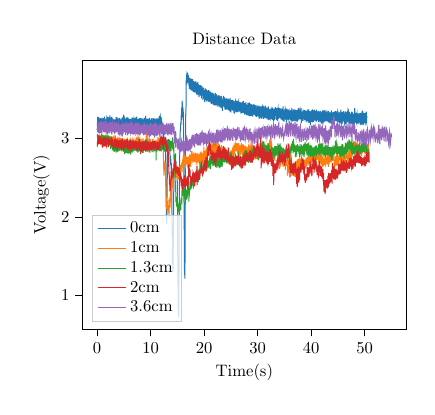
\begin{tikzpicture}[scale=0.6]

    \definecolor{crimson2143940}{RGB}{214,39,40}
    \definecolor{darkgray176}{RGB}{176,176,176}
    \definecolor{darkorange25512714}{RGB}{255,127,14}
    \definecolor{forestgreen4416044}{RGB}{44,160,44}
    \definecolor{lightgray204}{RGB}{204,204,204}
    \definecolor{mediumpurple148103189}{RGB}{148,103,189}
    \definecolor{steelblue31119180}{RGB}{31,119,180}

    \begin{axis}[
            legend cell align={left},
            legend style={
                    fill opacity=0.8,
                    draw opacity=1,
                    text opacity=1,
                    at={(0.03,0.03)},
                    anchor=south west,
                    draw=lightgray204
                },
            tick align=outside,
            tick pos=left,
            title={Distance Data},
            x grid style={darkgray176},
            xlabel={Time(s)},
            xmin=-2.7275, xmax=57.7835,
            xtick style={color=black},
            y grid style={darkgray176},
            ylabel={Voltage(V)},
            ymin=0.562316715542522, ymax=3.99780058651026,
            ytick style={color=black}
        ]
        \addplot [semithick, steelblue31119180]
        table {%
                0.024 3.11339198435973
                0.063 3.12805474095797
                0.096 3.26979472140762
                0.134 3.26979472140762
                0.165 3.10850439882698
                0.198 3.2355816226784
                0.23 3.24046920821114
                0.263 3.13782991202346
                0.295 3.27468230694037
                0.327 3.16715542521994
                0.36 3.20625610948192
                0.392 3.25513196480938
                0.424 3.12316715542522
                0.456 3.25513196480938
                0.489 3.23069403714565
                0.522 3.13294232649071
                0.553 3.26001955034213
                0.586 3.18670576735093
                0.618 3.21603128054741
                0.651 3.24046920821114
                0.684 3.11827956989247
                0.715 3.26490713587488
                0.748 3.22091886608016
                0.78 3.14760508308895
                0.813 3.25513196480938
                0.844 3.14271749755621
                0.877 3.2258064516129
                0.91 3.25513196480938
                0.942 3.12805474095797
                0.974 3.24046920821114
                1.007 3.2258064516129
                1.039 3.13294232649071
                1.072 3.26490713587488
                1.103 3.14271749755621
                1.137 3.20625610948192
                1.169 3.26490713587488
                1.202 3.12805474095797
                1.234 3.23069403714565
                1.266 3.23069403714565
                1.299 3.11827956989247
                1.331 3.25024437927664
                1.363 3.16715542521994
                1.396 3.19648093841642
                1.428 3.27956989247312
                1.461 3.10850439882698
                1.492 3.21603128054741
                1.525 3.21114369501466
                1.557 3.14271749755621
                1.59 3.24535679374389
                1.623 3.14271749755621
                1.654 3.18670576735093
                1.687 3.24046920821114
                1.719 3.12805474095797
                1.752 3.25513196480938
                1.784 3.21603128054741
                1.819 3.12805474095797
                1.851 3.26001955034213
                1.884 3.25024437927664
                1.916 3.13294232649071
                1.949 3.25513196480938
                1.981 3.19159335288368
                2.014 3.17204301075269
                2.046 3.27468230694037
                2.079 3.12316715542522
                2.112 3.20625610948192
                2.145 3.23069403714565
                2.178 3.11339198435973
                2.209 3.25024437927664
                2.242 3.23069403714565
                2.275 3.13294232649071
                2.308 3.26979472140762
                2.339 3.16715542521994
                2.372 3.16715542521994
                2.405 3.29423264907136
                2.438 3.15738025415445
                2.469 3.2355816226784
                2.502 3.25513196480938
                2.535 3.12316715542522
                2.567 3.26001955034213
                2.599 3.18181818181818
                2.632 3.16715542521994
                2.665 3.27468230694037
                2.697 3.17204301075269
                2.729 3.24046920821114
                2.762 3.27468230694037
                2.794 3.12805474095797
                2.827 3.26001955034213
                2.86 3.20136852394917
                2.892 3.12805474095797
                2.924 3.25513196480938
                2.957 3.14760508308895
                2.99 3.19159335288368
                3.021 3.24046920821114
                3.054 3.12316715542522
                3.087 3.24535679374389
                3.121 3.21603128054741
                3.152 3.12805474095797
                3.185 3.2355816226784
                3.218 3.20136852394917
                3.251 3.12805474095797
                3.282 3.24535679374389
                3.315 3.16715542521994
                3.348 3.19159335288368
                3.38 3.23069403714565
                3.412 3.13294232649071
                3.445 3.22091886608016
                3.48 3.24046920821114
                3.513 3.13782991202346
                3.546 3.27468230694037
                3.577 3.24046920821114
                3.61 3.12805474095797
                3.643 3.24046920821114
                3.676 3.18670576735093
                3.707 3.1524926686217
                3.74 3.26979472140762
                3.773 3.15738025415445
                3.805 3.20136852394917
                3.837 3.25513196480938
                3.87 3.10850439882698
                3.903 3.23069403714565
                3.935 3.21603128054741
                3.968 3.12805474095797
                4 3.25513196480938
                4.033 3.15738025415445
                4.065 3.16715542521994
                4.098 3.25024437927664
                4.131 3.16715542521994
                4.163 3.21114369501466
                4.196 3.26490713587488
                4.229 3.09872922776149
                4.261 3.25024437927664
                4.293 3.18181818181818
                4.326 3.11827956989247
                4.359 3.24535679374389
                4.39 3.15738025415445
                4.423 3.20136852394917
                4.456 3.24535679374389
                4.489 3.10361681329423
                4.52 3.21114369501466
                4.553 3.22091886608016
                4.586 3.13294232649071
                4.618 3.24046920821114
                4.651 3.17204301075269
                4.683 3.13782991202346
                4.716 3.26490713587488
                4.748 3.12316715542522
                4.781 3.2258064516129
                4.813 3.27468230694037
                4.845 3.12316715542522
                4.878 3.25513196480938
                4.911 3.20136852394917
                4.943 3.13782991202346
                4.975 3.30400782013685
                5.008 3.12805474095797
                5.041 3.20625610948192
                5.072 3.28445747800587
                5.105 3.08895405669599
                5.141 3.17693059628543
                5.174 3.26490713587488
                5.207 3.1524926686217
                5.239 3.2258064516129
                5.271 3.24046920821114
                5.304 3.11339198435973
                5.337 3.24046920821114
                5.368 3.2258064516129
                5.401 3.15738025415445
                5.434 3.25024437927664
                5.467 3.1524926686217
                5.498 3.22091886608016
                5.531 3.26979472140762
                5.564 3.12316715542522
                5.596 3.2258064516129
                5.628 3.21114369501466
                5.661 3.13782991202346
                5.694 3.26979472140762
                5.726 3.18670576735093
                5.758 3.18181818181818
                5.791 3.26490713587488
                5.823 3.12805474095797
                5.856 3.25024437927664
                5.889 3.22091886608016
                5.92 3.11827956989247
                5.953 3.25024437927664
                5.986 3.15738025415445
                6.019 3.16226783968719
                6.05 3.24535679374389
                6.083 3.16226783968719
                6.117 3.20136852394917
                6.149 3.25024437927664
                6.181 3.11827956989247
                6.214 3.2355816226784
                6.247 3.21603128054741
                6.279 3.11827956989247
                6.311 3.25024437927664
                6.344 3.15738025415445
                6.376 3.18181818181818
                6.409 3.24046920821114
                6.441 3.11827956989247
                6.473 3.23069403714565
                6.506 3.21603128054741
                6.539 3.09872922776149
                6.572 3.26979472140762
                6.604 3.19648093841642
                6.636 3.13294232649071
                6.669 3.26001955034213
                6.702 3.15738025415445
                6.733 3.19159335288368
                6.766 3.25513196480938
                6.799 3.11827956989247
                6.834 3.21114369501466
                6.866 3.24535679374389
                6.898 3.10850439882698
                6.931 3.24046920821114
                6.964 3.23069403714565
                6.996 3.14760508308895
                7.028 3.24535679374389
                7.061 3.17693059628543
                7.094 3.16715542521994
                7.127 3.26490713587488
                7.159 3.17693059628543
                7.192 3.24535679374389
                7.225 3.26490713587488
                7.257 3.12316715542522
                7.289 3.2355816226784
                7.322 3.21114369501466
                7.354 3.12316715542522
                7.387 3.27956989247312
                7.419 3.16715542521994
                7.452 3.21603128054741
                7.484 3.25024437927664
                7.517 3.16715542521994
                7.549 3.2258064516129
                7.582 3.2258064516129
                7.614 3.12805474095797
                7.647 3.24535679374389
                7.68 3.21603128054741
                7.711 3.14271749755621
                7.744 3.25024437927664
                7.777 3.13782991202346
                7.81 3.21114369501466
                7.841 3.25024437927664
                7.874 3.09384164222874
                7.907 3.26001955034213
                7.939 3.18181818181818
                7.971 3.10361681329423
                8.004 3.25024437927664
                8.036 3.15738025415445
                8.069 3.18670576735093
                8.101 3.26001955034213
                8.135 3.11339198435973
                8.167 3.21114369501466
                8.2 3.24535679374389
                8.232 3.12316715542522
                8.264 3.24046920821114
                8.297 3.18670576735093
                8.33 3.13782991202346
                8.363 3.26490713587488
                8.394 3.12805474095797
                8.427 3.18670576735093
                8.46 3.25024437927664
                8.495 3.13782991202346
                8.527 3.20625610948192
                8.56 3.24535679374389
                8.592 3.11827956989247
                8.625 3.24046920821114
                8.657 3.22091886608016
                8.689 3.09872922776149
                8.722 3.24046920821114
                8.755 3.16226783968719
                8.787 3.19159335288368
                8.819 3.26490713587488
                8.852 3.11827956989247
                8.885 3.21114369501466
                8.916 3.25024437927664
                8.949 3.10850439882698
                8.982 3.21114369501466
                9.015 3.19159335288368
                9.047 3.12805474095797
                9.079 3.28934506353861
                9.113 3.16715542521994
                9.146 3.17693059628543
                9.178 3.24535679374389
                9.21 3.11339198435973
                9.243 3.2355816226784
                9.275 3.23069403714565
                9.308 3.08406647116325
                9.34 3.24535679374389
                9.373 3.19648093841642
                9.405 3.13294232649071
                9.438 3.25513196480938
                9.47 3.13294232649071
                9.502 3.19648093841642
                9.535 3.25024437927664
                9.568 3.10850439882698
                9.601 3.2258064516129
                9.632 3.20136852394917
                9.665 3.13294232649071
                9.698 3.2355816226784
                9.731 3.16715542521994
                9.762 3.17693059628543
                9.795 3.26490713587488
                9.828 3.10850439882698
                9.861 3.2258064516129
                9.892 3.24046920821114
                9.925 3.11827956989247
                9.958 3.24046920821114
                9.991 3.17204301075269
                10.022 3.14271749755621
                10.055 3.24046920821114
                10.088 3.14271749755621
                10.122 3.18181818181818
                10.157 3.25513196480938
                10.189 3.18670576735093
                10.222 3.12805474095797
                10.254 3.26001955034213
                10.287 3.15738025415445
                10.319 3.19159335288368
                10.352 3.24046920821114
                10.384 3.10850439882698
                10.417 3.24046920821114
                10.449 3.22091886608016
                10.482 3.09872922776149
                10.514 3.26001955034213
                10.547 3.16226783968719
                10.579 3.16715542521994
                10.612 3.25513196480938
                10.644 3.10361681329423
                10.677 3.22091886608016
                10.71 3.22091886608016
                10.742 3.11339198435973
                10.774 3.21114369501466
                10.807 3.14271749755621
                10.84 3.14271749755621
                10.872 3.25513196480938
                10.904 3.13782991202346
                10.937 3.19648093841642
                10.97 3.2355816226784
                11.002 3.09872922776149
                11.034 3.25024437927664
                11.067 3.19159335288368
                11.1 3.10850439882698
                11.133 3.2355816226784
                11.165 3.17693059628543
                11.198 3.13294232649071
                11.231 3.26490713587488
                11.264 3.12805474095797
                11.295 3.20136852394917
                11.328 3.24535679374389
                11.361 3.08895405669599
                11.394 3.24535679374389
                11.425 3.23069403714565
                11.458 3.12805474095797
                11.491 3.25513196480938
                11.524 3.19159335288368
                11.555 3.19648093841642
                11.588 3.27956989247312
                11.621 3.1524926686217
                11.656 3.16715542521994
                11.688 3.28934506353861
                11.72 3.1524926686217
                11.753 3.26979472140762
                11.786 3.27956989247312
                11.817 3.14271749755621
                11.85 3.28445747800587
                11.883 3.21603128054741
                11.915 3.20625610948192
                11.948 3.27956989247312
                11.979 3.15738025415445
                12.012 3.25513196480938
                12.045 3.23069403714565
                12.077 3.11827956989247
                12.11 3.21114369501466
                12.143 3.16715542521994
                12.175 3.069403714565
                12.208 3.19648093841642
                12.239 3.05474095796676
                12.272 3.09872922776149
                12.305 3.14760508308895
                12.337 3.0058651026393
                12.369 3.14271749755621
                12.402 3.069403714565
                12.434 2.94721407624633
                12.467 3.09872922776149
                12.498 2.94232649071359
                12.531 2.98631476050831
                12.564 3.01075268817204
                12.596 2.84457478005865
                12.628 2.97653958944282
                12.661 2.9227761485826
                12.693 2.82991202346041
                12.726 2.92766373411535
                12.758 2.83479960899316
                12.79 2.82991202346041
                12.823 2.80547409579668
                12.855 2.51710654936461
                12.888 2.36559139784946
                12.92 2.18963831867058
                12.952 1.97947214076246
                12.985 1.96480938416422
                13.017 1.91104594330401
                13.049 2.04301075268817
                13.082 2.34115347018573
                13.115 2.47311827956989
                13.148 2.7663734115347
                13.182 2.82502443792766
                13.215 2.80547409579668
                13.248 2.89345063538612
                13.28 2.91788856304985
                13.313 2.86412512218964
                13.344 2.9960899315738
                13.377 2.95698924731183
                13.41 2.88856304985337
                13.442 2.97165200391007
                13.474 2.86412512218964
                13.507 2.94721407624633
                13.539 2.98142717497556
                13.572 2.84457478005865
                13.603 2.88367546432063
                13.636 2.7761485826002
                13.669 2.6930596285435
                13.701 2.7761485826002
                13.733 2.66373411534702
                13.766 2.71749755620723
                13.798 2.73704789833822
                13.831 2.6099706744868
                13.862 2.6930596285435
                13.895 2.55131964809384
                13.928 2.46823069403715
                13.96 2.49266862170088
                13.992 2.14076246334311
                14.025 1.88172043010753
                14.057 1.72043010752688
                14.09 1.39784946236559
                14.123 1.48093841642229
                14.155 1.3782991202346
                14.188 1.29032258064516
                14.22 1.55913978494624
                14.253 1.67644183773216
                14.285 1.9208211143695
                14.317 2.29227761485826
                14.35 2.35581622678397
                14.382 2.52688172043011
                14.414 2.56598240469208
                14.447 2.55131964809384
                14.479 2.78103616813294
                14.512 2.76148582600196
                14.544 2.75171065493646
                14.576 2.7663734115347
                14.609 2.65395894428152
                14.641 2.79081133919844
                14.676 2.81036168132942
                14.708 2.70283479960899
                14.741 2.66862170087977
                14.774 2.67350928641251
                14.807 2.53176930596285
                14.838 2.63929618768328
                14.871 2.57086999022483
                14.904 2.50733137829912
                14.937 2.56109481915934
                14.968 2.43890518084066
                15.001 2.48289345063539
                15.034 2.11143695014663
                15.067 1.57869012707722
                15.098 1.33919843597263
                15.132 1.08504398826979
                15.165 0.826001955034213
                15.198 0.821114369501466
                15.229 0.733137829912023
                15.262 0.718475073313783
                15.295 1.06060606060606
                15.328 1.41251221896383
                15.36 2.02834799608993
                15.392 2.56109481915934
                15.425 2.69794721407625
                15.458 2.89345063538612
                15.491 2.96187683284457
                15.522 2.97653958944282
                15.555 3.12805474095797
                15.588 3.10361681329423
                15.621 3.15738025415445
                15.652 3.21114369501466
                15.685 3.17693059628543
                15.718 3.26979472140762
                15.751 3.31867057673509
                15.782 3.2355816226784
                15.815 3.38709677419355
                15.848 3.38709677419355
                15.881 3.33822091886608
                15.912 3.48484848484848
                15.945 3.3822091886608
                15.978 3.36265884652981
                16.011 3.41642228739003
                16.043 3.26979472140762
                16.075 3.37732160312805
                16.108 3.33822091886608
                16.142 3.16715542521994
                16.174 3.20136852394917
                16.209 2.72238514173998
                16.242 2.22873900293255
                16.275 1.9941348973607
                16.307 1.72531769305963
                16.339 1.32453567937439
                16.372 1.29032258064516
                16.405 1.21212121212121
                16.438 1.43695014662757
                16.47 1.98924731182796
                16.502 2.52688172043011
                16.535 3.02052785923754
                16.568 3.29912023460411
                16.601 3.29912023460411
                16.637 3.47507331378299
                16.669 3.75855327468231
                16.702 3.72922776148583
                16.735 3.7683284457478
                16.768 3.83186705767351
                16.799 3.69012707722385
                16.832 3.81231671554252
                16.865 3.80254154447703
                16.898 3.71456500488759
                16.93 3.841642228739
                16.962 3.74877810361681
                16.995 3.71945259042033
                17.028 3.81231671554252
                17.06 3.71456500488759
                17.093 3.74877810361681
                17.126 3.80742913000978
                17.159 3.67546432062561
                17.191 3.75855327468231
                17.224 3.75855327468231
                17.256 3.63147605083089
                17.289 3.77321603128055
                17.321 3.72922776148583
                17.354 3.63147605083089
                17.387 3.77321603128055
                17.419 3.67057673509286
                17.452 3.71456500488759
                17.484 3.74877810361681
                17.517 3.61681329423265
                17.55 3.72434017595308
                17.583 3.74389051808407
                17.614 3.62658846529814
                17.647 3.75855327468231
                17.68 3.70478983382209
                17.715 3.6119257086999
                17.747 3.72434017595308
                17.78 3.71456500488759
                17.812 3.61681329423265
                17.845 3.75855327468231
                17.878 3.65102639296188
                17.91 3.67546432062561
                17.942 3.72922776148583
                17.975 3.59726295210166
                18.008 3.70967741935484
                18.04 3.73411534701857
                18.072 3.59237536656891
                18.105 3.73411534701857
                18.139 3.6852394916911
                18.171 3.60215053763441
                18.203 3.72434017595308
                18.236 3.6119257086999
                18.269 3.65591397849462
                18.301 3.71945259042033
                18.333 3.58748778103617
                18.366 3.71456500488759
                18.399 3.6950146627566
                18.432 3.58748778103617
                18.463 3.73411534701857
                18.496 3.65591397849462
                18.529 3.63147605083089
                18.562 3.70967741935484
                18.593 3.56793743890518
                18.626 3.65591397849462
                18.659 3.66568914956012
                18.692 3.55327468230694
                18.723 3.6852394916911
                18.756 3.64613880742913
                18.789 3.56304985337243
                18.822 3.71945259042033
                18.853 3.57282502443793
                18.886 3.62658846529814
                18.919 3.69012707722385
                18.952 3.58260019550342
                18.983 3.67546432062561
                19.016 3.64613880742913
                19.049 3.52883675464321
                19.082 3.66568914956012
                19.113 3.6119257086999
                19.147 3.59237536656891
                19.18 3.68035190615836
                19.213 3.60215053763441
                19.248 3.55327468230694
                19.28 3.67057673509286
                19.312 3.57771260997067
                19.345 3.60703812316716
                19.378 3.68035190615836
                19.41 3.54349951124145
                19.442 3.61681329423265
                19.475 3.66568914956012
                19.508 3.51417399804497
                19.54 3.66568914956012
                19.572 3.6119257086999
                19.605 3.55816226783969
                19.638 3.66568914956012
                19.671 3.54838709677419
                19.702 3.60703812316716
                19.735 3.64613880742913
                19.768 3.49462365591398
                19.801 3.62658846529814
                19.832 3.6119257086999
                19.865 3.50928641251222
                19.898 3.65102639296188
                19.931 3.56793743890518
                19.962 3.56304985337243
                19.995 3.61681329423265
                20.028 3.57282502443793
                20.061 3.60703812316716
                20.092 3.60703812316716
                20.126 3.4652981427175
                20.159 3.6119257086999
                20.192 3.58260019550342
                20.224 3.50439882697947
                20.256 3.64125122189638
                20.289 3.50928641251222
                20.322 3.56793743890518
                20.354 3.61681329423265
                20.386 3.49462365591398
                20.419 3.58748778103617
                20.451 3.62658846529814
                20.484 3.47507331378299
                20.516 3.6119257086999
                20.549 3.55327468230694
                20.581 3.48973607038123
                20.614 3.60703812316716
                20.646 3.49951124144673
                20.679 3.56793743890518
                20.711 3.6119257086999
                20.744 3.47018572825024
                20.774 3.58748778103617
                20.807 3.5386119257087
                20.839 3.52394916911046
                20.872 3.6217008797654
                20.904 3.48484848484848
                20.937 3.55816226783969
                20.969 3.60215053763441
                21.002 3.4652981427175
                21.035 3.58260019550342
                21.067 3.52394916911046
                21.099 3.47507331378299
                21.133 3.57771260997067
                21.166 3.51906158357771
                21.198 3.50439882697947
                21.23 3.59237536656891
                21.263 3.45063538611926
                21.296 3.56304985337243
                21.328 3.55327468230694
                21.36 3.44086021505376
                21.393 3.56304985337243
                21.426 3.51417399804497
                21.458 3.47507331378299
                21.49 3.58748778103617
                21.523 3.49462365591398
                21.556 3.53372434017595
                21.588 3.57282502443793
                21.62 3.44574780058651
                21.653 3.55816226783969
                21.686 3.52883675464321
                21.719 3.43108504398827
                21.75 3.57771260997067
                21.783 3.48973607038123
                21.816 3.46041055718475
                21.849 3.57282502443793
                21.88 3.42619745845552
                21.913 3.53372434017595
                21.946 3.53372434017595
                21.979 3.42619745845552
                22.011 3.54838709677419
                22.043 3.51417399804497
                22.076 3.42130987292278
                22.109 3.58260019550342
                22.141 3.48973607038123
                22.174 3.46041055718475
                22.207 3.56793743890518
                22.24 3.43108504398827
                22.275 3.46041055718475
                22.307 3.56304985337243
                22.34 3.51417399804497
                22.372 3.49462365591398
                22.405 3.55816226783969
                22.437 3.40664711632454
                22.47 3.52883675464321
                22.503 3.52394916911046
                22.535 3.42619745845552
                22.567 3.5386119257087
                22.6 3.46041055718475
                22.633 3.4652981427175
                22.665 3.54838709677419
                22.697 3.42130987292278
                22.73 3.50928641251222
                22.763 3.55327468230694
                22.795 3.40175953079179
                22.828 3.53372434017595
                22.86 3.46041055718475
                22.893 3.41642228739003
                22.925 3.54349951124145
                22.958 3.45063538611926
                22.99 3.47018572825024
                23.023 3.5386119257087
                23.055 3.41153470185728
                23.088 3.49462365591398
                23.12 3.49462365591398
                23.154 3.38709677419355
                23.187 3.50928641251222
                23.219 3.45063538611926
                23.251 3.3919843597263
                23.284 3.54349951124145
                23.317 3.43597262952102
                23.349 3.46041055718475
                23.382 3.51906158357771
                23.414 3.35288367546432
                23.447 3.47018572825024
                23.479 3.49462365591398
                23.512 3.40664711632454
                23.544 3.48973607038123
                23.577 3.44086021505376
                23.609 3.40664711632454
                23.642 3.54349951124145
                23.674 3.42130987292278
                23.707 3.47018572825024
                23.74 3.50439882697947
                23.772 3.40175953079179
                23.808 3.47507331378299
                23.839 3.52394916911046
                23.872 3.37243401759531
                23.904 3.49462365591398
                23.937 3.46041055718475
                23.969 3.36754643206256
                24.001 3.50928641251222
                24.034 3.41153470185728
                24.067 3.43108504398827
                24.098 3.50439882697947
                24.132 3.37243401759531
                24.164 3.47018572825024
                24.197 3.48484848484848
                24.229 3.36754643206256
                24.261 3.51417399804497
                24.294 3.44574780058651
                24.327 3.42130987292278
                24.358 3.47996089931574
                24.391 3.3822091886608
                24.423 3.47996089931574
                24.456 3.49462365591398
                24.488 3.36265884652981
                24.52 3.50928641251222
                24.553 3.43108504398827
                24.586 3.37732160312805
                24.617 3.49951124144673
                24.65 3.36754643206256
                24.682 3.47996089931574
                24.715 3.49462365591398
                24.748 3.35288367546432
                24.779 3.47996089931574
                24.812 3.41642228739003
                24.845 3.38709677419355
                24.877 3.51906158357771
                24.909 3.33333333333333
                24.941 3.4652981427175
                24.974 3.48484848484848
                25.007 3.33333333333333
                25.038 3.48973607038123
                25.071 3.41153470185728
                25.104 3.38709677419355
                25.137 3.48973607038123
                25.169 3.36754643206256
                25.202 3.41642228739003
                25.234 3.47996089931574
                25.267 3.35777126099707
                25.309 3.40175953079179
                25.344 3.37243401759531
                25.378 3.49462365591398
                25.413 3.47507331378299
                25.447 3.36265884652981
                25.482 3.3919843597263
                25.517 3.47996089931574
                25.551 3.44574780058651
                25.585 3.32844574780059
                25.62 3.43108504398827
                25.655 3.47507331378299
                25.689 3.41153470185728
                25.723 3.31867057673509
                25.758 3.43108504398827
                25.793 3.455522971652
                25.827 3.36754643206256
                25.862 3.34310850439883
                25.896 3.47018572825024
                25.931 3.46041055718475
                25.965 3.34310850439883
                26 3.37243401759531
                26.035 3.47996089931574
                26.068 3.4652981427175
                26.103 3.33333333333333
                26.138 3.42619745845552
                26.173 3.48484848484848
                26.208 3.43108504398827
                26.243 3.34310850439883
                26.276 3.44574780058651
                26.311 3.47507331378299
                26.346 3.41642228739003
                26.381 3.33822091886608
                26.415 3.46041055718475
                26.449 3.47018572825024
                26.484 3.37243401759531
                26.519 3.37243401759531
                26.553 3.4652981427175
                26.588 3.45063538611926
                26.622 3.34310850439883
                26.656 3.3822091886608
                26.691 3.4652981427175
                26.726 3.43108504398827
                26.761 3.35288367546432
                26.795 3.40664711632454
                26.829 3.46041055718475
                26.864 3.40175953079179
                26.899 3.31867057673509
                26.936 3.3822091886608
                26.971 3.46041055718475
                27.005 3.43597262952102
                27.039 3.32355816226784
                27.074 3.39687194525904
                27.109 3.46041055718475
                27.144 3.42130987292278
                27.179 3.32844574780059
                27.213 3.40664711632454
                27.248 3.47507331378299
                27.283 3.39687194525904
                27.318 3.32844574780059
                27.353 3.42130987292278
                27.387 3.47996089931574
                27.422 3.36265884652981
                27.457 3.32355816226784
                27.491 3.40175953079179
                27.526 3.45063538611926
                27.56 3.36265884652981
                27.595 3.30400782013685
                27.63 3.43108504398827
                27.665 3.45063538611926
                27.7 3.31378299120235
                27.734 3.34310850439883
                27.768 3.42619745845552
                27.803 3.4652981427175
                27.838 3.3088954056696
                27.873 3.33822091886608
                27.908 3.43597262952102
                27.942 3.41642228739003
                27.976 3.29423264907136
                28.011 3.36754643206256
                28.046 3.42619745845552
                28.081 3.40175953079179
                28.115 3.29912023460411
                28.15 3.38709677419355
                28.185 3.455522971652
                28.219 3.38709677419355
                28.254 3.30400782013685
                28.29 3.39687194525904
                28.324 3.455522971652
                28.359 3.42619745845552
                28.394 3.28934506353861
                28.428 3.40664711632454
                28.463 3.455522971652
                28.497 3.3822091886608
                28.535 3.28445747800587
                28.57 3.35288367546432
                28.604 3.42130987292278
                28.639 3.41153470185728
                28.674 3.34799608993157
                28.708 3.37243401759531
                28.743 3.44086021505376
                28.778 3.40175953079179
                28.812 3.28934506353861
                28.847 3.37243401759531
                28.881 3.43597262952102
                28.916 3.35777126099707
                28.951 3.28934506353861
                28.986 3.40175953079179
                29.021 3.42619745845552
                29.054 3.32355816226784
                29.089 3.27956989247312
                29.124 3.40175953079179
                29.159 3.43108504398827
                29.194 3.3088954056696
                29.229 3.3088954056696
                29.263 3.41153470185728
                29.297 3.44086021505376
                29.332 3.33333333333333
                29.368 3.3088954056696
                29.403 3.41642228739003
                29.437 3.41153470185728
                29.472 3.31867057673509
                29.506 3.32355816226784
                29.541 3.42130987292278
                29.576 3.40664711632454
                29.611 3.28934506353861
                29.645 3.32355816226784
                29.68 3.42619745845552
                29.715 3.3919843597263
                29.749 3.27468230694037
                29.784 3.36265884652981
                29.818 3.39687194525904
                29.853 3.36754643206256
                29.888 3.28445747800587
                29.923 3.37243401759531
                29.958 3.42130987292278
                29.991 3.34310850439883
                30.026 3.29912023460411
                30.061 3.37732160312805
                30.096 3.41153470185728
                30.131 3.35288367546432
                30.168 3.27956989247312
                30.202 3.34310850439883
                30.237 3.42130987292278
                30.272 3.38709677419355
                30.307 3.25024437927664
                30.341 3.35288367546432
                30.375 3.41153470185728
                30.411 3.36754643206256
                30.446 3.26001955034213
                30.481 3.36754643206256
                30.515 3.40175953079179
                30.55 3.35777126099707
                30.584 3.26979472140762
                30.619 3.3919843597263
                30.654 3.41153470185728
                30.689 3.28934506353861
                30.723 3.25513196480938
                30.757 3.3822091886608
                30.792 3.3822091886608
                30.827 3.3088954056696
                30.862 3.28445747800587
                30.897 3.3919843597263
                30.93 3.42130987292278
                30.965 3.30400782013685
                31 3.31378299120235
                31.035 3.39687194525904
                31.07 3.38709677419355
                31.105 3.25024437927664
                31.138 3.31867057673509
                31.173 3.41153470185728
                31.208 3.35777126099707
                31.243 3.27468230694037
                31.278 3.33333333333333
                31.312 3.3919843597263
                31.347 3.36265884652981
                31.381 3.26001955034213
                31.416 3.37243401759531
                31.451 3.42130987292278
                31.486 3.34799608993157
                31.521 3.28445747800587
                31.555 3.31378299120235
                31.59 3.38709677419355
                31.625 3.32844574780059
                31.66 3.25513196480938
                31.694 3.35777126099707
                31.729 3.39687194525904
                31.766 3.37243401759531
                31.801 3.26001955034213
                31.836 3.32355816226784
                31.87 3.3822091886608
                31.904 3.32844574780059
                31.939 3.24046920821114
                31.974 3.35288367546432
                32.009 3.41153470185728
                32.044 3.32844574780059
                32.078 3.2355816226784
                32.112 3.36265884652981
                32.147 3.37732160312805
                32.182 3.29912023460411
                32.217 3.24046920821114
                32.251 3.35288367546432
                32.286 3.36754643206256
                32.32 3.27956989247312
                32.355 3.26979472140762
                32.39 3.34799608993157
                32.424 3.3822091886608
                32.459 3.25513196480938
                32.494 3.28934506353861
                32.528 3.35777126099707
                32.564 3.37732160312805
                32.599 3.25024437927664
                32.633 3.27468230694037
                32.667 3.36265884652981
                32.702 3.35288367546432
                32.737 3.2355816226784
                32.772 3.30400782013685
                32.806 3.37732160312805
                32.841 3.37243401759531
                32.876 3.24046920821114
                32.91 3.32355816226784
                32.945 3.3822091886608
                32.979 3.31867057673509
                33.014 3.21603128054741
                33.049 3.34799608993157
                33.084 3.3822091886608
                33.118 3.26490713587488
                33.153 3.2355816226784
                33.187 3.36265884652981
                33.222 3.37732160312805
                33.257 3.29912023460411
                33.292 3.25024437927664
                33.327 3.40175953079179
                33.361 3.36754643206256
                33.398 3.3919843597263
                33.433 3.29423264907136
                33.468 3.32844574780059
                33.503 3.3822091886608
                33.538 3.32844574780059
                33.572 3.2355816226784
                33.607 3.3088954056696
                33.647 3.38709677419355
                33.681 3.35777126099707
                33.716 3.29423264907136
                33.751 3.2258064516129
                33.785 3.37243401759531
                33.82 3.38709677419355
                33.855 3.34310850439883
                33.89 3.25024437927664
                33.924 3.34310850439883
                33.958 3.37243401759531
                33.993 3.27468230694037
                34.028 3.26001955034213
                34.063 3.3919843597263
                34.098 3.35777126099707
                34.132 3.28934506353861
                34.167 3.28445747800587
                34.202 3.38709677419355
                34.237 3.36265884652981
                34.271 3.27468230694037
                34.306 3.28934506353861
                34.34 3.37243401759531
                34.375 3.34799608993157
                34.41 3.24046920821114
                34.445 3.33333333333333
                34.48 3.3822091886608
                34.514 3.33822091886608
                34.549 3.24046920821114
                34.584 3.3088954056696
                34.618 3.37732160312805
                34.653 3.33333333333333
                34.689 3.23069403714565
                34.723 3.30400782013685
                34.758 3.41153470185728
                34.792 3.34310850439883
                34.827 3.22091886608016
                34.862 3.33822091886608
                34.896 3.35777126099707
                34.931 3.31378299120235
                34.966 3.21603128054741
                35.003 3.27468230694037
                35.038 3.35777126099707
                35.073 3.36265884652981
                35.107 3.30400782013685
                35.142 3.3088954056696
                35.177 3.36754643206256
                35.212 3.35288367546432
                35.246 3.24046920821114
                35.28 3.31378299120235
                35.315 3.3822091886608
                35.35 3.32844574780059
                35.385 3.20625610948192
                35.42 3.32355816226784
                35.454 3.3822091886608
                35.488 3.28934506353861
                35.523 3.24046920821114
                35.558 3.29423264907136
                35.593 3.36754643206256
                35.628 3.26490713587488
                35.662 3.25513196480938
                35.697 3.33822091886608
                35.732 3.36754643206256
                35.767 3.28445747800587
                35.802 3.2355816226784
                35.836 3.33822091886608
                35.871 3.34799608993157
                35.906 3.27468230694037
                35.94 3.24535679374389
                35.975 3.33822091886608
                36.009 3.33822091886608
                36.044 3.26979472140762
                36.079 3.24535679374389
                36.114 3.34310850439883
                36.149 3.33822091886608
                36.183 3.23069403714565
                36.217 3.26979472140762
                36.252 3.36265884652981
                36.287 3.34310850439883
                36.322 3.22091886608016
                36.357 3.30400782013685
                36.391 3.38709677419355
                36.425 3.32844574780059
                36.46 3.2258064516129
                36.495 3.31867057673509
                36.53 3.35288367546432
                36.564 3.29423264907136
                36.599 3.21603128054741
                36.636 3.24535679374389
                36.671 3.37243401759531
                36.706 3.33822091886608
                36.74 3.24046920821114
                36.774 3.3088954056696
                36.81 3.37243401759531
                36.844 3.34310850439883
                36.879 3.22091886608016
                36.914 3.31378299120235
                36.947 3.36265884652981
                36.982 3.3088954056696
                37.017 3.22091886608016
                37.052 3.31378299120235
                37.086 3.35777126099707
                37.121 3.27468230694037
                37.155 3.22091886608016
                37.19 3.34799608993157
                37.224 3.34310850439883
                37.259 3.24535679374389
                37.294 3.26001955034213
                37.327 3.36265884652981
                37.362 3.32844574780059
                37.397 3.21114369501466
                37.432 3.31378299120235
                37.466 3.34799608993157
                37.5 3.28934506353861
                37.535 3.22091886608016
                37.57 3.32844574780059
                37.604 3.38709677419355
                37.639 3.28445747800587
                37.673 3.24046920821114
                37.707 3.32355816226784
                37.742 3.34799608993157
                37.777 3.24535679374389
                37.812 3.28445747800587
                37.846 3.35777126099707
                37.881 3.36754643206256
                37.916 3.24535679374389
                37.95 3.29423264907136
                37.985 3.33333333333333
                38.02 3.32844574780059
                38.054 3.24535679374389
                38.088 3.3088954056696
                38.123 3.3919843597263
                38.158 3.27956989247312
                38.192 3.19648093841642
                38.226 3.33822091886608
                38.259 3.33822091886608
                38.293 3.22091886608016
                38.328 3.26979472140762
                38.363 3.34310850439883
                38.397 3.31378299120235
                38.431 3.22091886608016
                38.466 3.32844574780059
                38.501 3.36754643206256
                38.536 3.28445747800587
                38.569 3.25513196480938
                38.604 3.35288367546432
                38.639 3.33822091886608
                38.674 3.25024437927664
                38.708 3.23069403714565
                38.743 3.34310850439883
                38.777 3.36265884652981
                38.811 3.2355816226784
                38.846 3.26490713587488
                38.881 3.36265884652981
                38.916 3.27956989247312
                38.95 3.24535679374389
                38.985 3.29912023460411
                39.02 3.34799608993157
                39.054 3.30400782013685
                39.089 3.20625610948192
                39.123 3.3088954056696
                39.157 3.35288367546432
                39.192 3.26979472140762
                39.227 3.2355816226784
                39.262 3.34310850439883
                39.296 3.34799608993157
                39.33 3.27468230694037
                39.365 3.2258064516129
                39.399 3.36754643206256
                39.434 3.32844574780059
                39.469 3.20625610948192
                39.503 3.26979472140762
                39.537 3.37243401759531
                39.572 3.31867057673509
                39.607 3.20136852394917
                39.641 3.28934506353861
                39.675 3.35288367546432
                39.71 3.26001955034213
                39.745 3.21114369501466
                39.779 3.31867057673509
                39.814 3.34310850439883
                39.851 3.3088954056696
                39.885 3.17204301075269
                39.92 3.27956989247312
                39.955 3.34799608993157
                39.99 3.28934506353861
                40.026 3.21603128054741
                40.06 3.29423264907136
                40.094 3.35777126099707
                40.129 3.3088954056696
                40.164 3.21114369501466
                40.199 3.29423264907136
                40.233 3.37243401759531
                40.268 3.27468230694037
                40.303 3.20625610948192
                40.337 3.33333333333333
                40.372 3.33822091886608
                40.407 3.26979472140762
                40.441 3.21114369501466
                40.476 3.33822091886608
                40.511 3.34310850439883
                40.546 3.26001955034213
                40.58 3.23069403714565
                40.614 3.33822091886608
                40.649 3.36754643206256
                40.684 3.24535679374389
                40.719 3.25024437927664
                40.754 3.34310850439883
                40.788 3.34310850439883
                40.823 3.24046920821114
                40.857 3.2355816226784
                40.892 3.35288367546432
                40.927 3.33822091886608
                40.962 3.21603128054741
                40.996 3.27468230694037
                41.031 3.36754643206256
                41.065 3.32355816226784
                41.101 3.23069403714565
                41.136 3.27956989247312
                41.17 3.32355816226784
                41.205 3.32844574780059
                41.24 3.2355816226784
                41.274 3.30400782013685
                41.309 3.34799608993157
                41.344 3.28934506353861
                41.378 3.21114369501466
                41.413 3.29423264907136
                41.448 3.34799608993157
                41.485 3.32355816226784
                41.52 3.24535679374389
                41.554 3.24535679374389
                41.589 3.31867057673509
                41.624 3.32355816226784
                41.659 3.20625610948192
                41.694 3.26490713587488
                41.728 3.35288367546432
                41.762 3.30400782013685
                41.797 3.21603128054741
                41.832 3.26490713587488
                41.867 3.33333333333333
                41.902 3.28934506353861
                41.935 3.19159335288368
                41.97 3.3088954056696
                42.005 3.34310850439883
                42.04 3.26490713587488
                42.075 3.20136852394917
                42.109 3.3088954056696
                42.144 3.35777126099707
                42.179 3.27956989247312
                42.214 3.17693059628543
                42.249 3.32844574780059
                42.284 3.35777126099707
                42.318 3.27468230694037
                42.353 3.20625610948192
                42.387 3.32355816226784
                42.422 3.35777126099707
                42.457 3.26490713587488
                42.491 3.2355816226784
                42.526 3.33333333333333
                42.561 3.33822091886608
                42.596 3.21603128054741
                42.63 3.23069403714565
                42.664 3.33822091886608
                42.699 3.33333333333333
                42.734 3.24046920821114
                42.769 3.25513196480938
                42.804 3.33333333333333
                42.839 3.3088954056696
                42.873 3.2258064516129
                42.907 3.26979472140762
                42.942 3.35777126099707
                42.977 3.32844574780059
                43.012 3.21603128054741
                43.046 3.29912023460411
                43.083 3.31378299120235
                43.118 3.33333333333333
                43.153 3.2355816226784
                43.188 3.23069403714565
                43.223 3.31867057673509
                43.257 3.35288367546432
                43.292 3.2355816226784
                43.327 3.20625610948192
                43.362 3.31867057673509
                43.397 3.33333333333333
                43.43 3.20136852394917
                43.465 3.24046920821114
                43.5 3.32355816226784
                43.535 3.29912023460411
                43.57 3.24046920821114
                43.604 3.29423264907136
                43.638 3.33333333333333
                43.673 3.30400782013685
                43.708 3.19159335288368
                43.743 3.29423264907136
                43.778 3.35777126099707
                43.812 3.27956989247312
                43.847 3.18670576735093
                43.882 3.3088954056696
                43.916 3.33333333333333
                43.951 3.26490713587488
                43.985 3.19159335288368
                44.02 3.32355816226784
                44.055 3.32355816226784
                44.09 3.24046920821114
                44.124 3.21114369501466
                44.158 3.32355816226784
                44.193 3.33822091886608
                44.228 3.24046920821114
                44.263 3.23069403714565
                44.298 3.30400782013685
                44.333 3.33333333333333
                44.367 3.24046920821114
                44.402 3.21114369501466
                44.437 3.3088954056696
                44.472 3.34799608993157
                44.506 3.2258064516129
                44.54 3.24046920821114
                44.575 3.35288367546432
                44.61 3.30400782013685
                44.645 3.23069403714565
                44.68 3.24535679374389
                44.717 3.29912023460411
                44.751 3.33333333333333
                44.786 3.2258064516129
                44.821 3.2258064516129
                44.856 3.32355816226784
                44.89 3.34799608993157
                44.924 3.23069403714565
                44.959 3.21603128054741
                44.994 3.34310850439883
                45.029 3.33333333333333
                45.064 3.20625610948192
                45.099 3.2258064516129
                45.132 3.32844574780059
                45.167 3.31378299120235
                45.202 3.20625610948192
                45.237 3.26490713587488
                45.272 3.33333333333333
                45.306 3.3088954056696
                45.341 3.20136852394917
                45.376 3.2355816226784
                45.411 3.33333333333333
                45.446 3.27468230694037
                45.48 3.19648093841642
                45.514 3.28445747800587
                45.549 3.36754643206256
                45.584 3.25513196480938
                45.619 3.19159335288368
                45.654 3.29912023460411
                45.688 3.32355816226784
                45.722 3.27468230694037
                45.757 3.18670576735093
                45.792 3.29912023460411
                45.827 3.33822091886608
                45.861 3.24046920821114
                45.896 3.20625610948192
                45.93 3.3088954056696
                45.965 3.32355816226784
                46 3.2355816226784
                46.034 3.24535679374389
                46.069 3.34799608993157
                46.104 3.31867057673509
                46.139 3.22091886608016
                46.173 3.25513196480938
                46.208 3.31867057673509
                46.242 3.29912023460411
                46.277 3.19648093841642
                46.314 3.1524926686217
                46.349 3.29423264907136
                46.384 3.34310850439883
                46.419 3.26001955034213
                46.454 3.18670576735093
                46.488 3.32355816226784
                46.523 3.31867057673509
                46.558 3.2258064516129
                46.593 3.20136852394917
                46.627 3.32355816226784
                46.662 3.32844574780059
                46.697 3.2355816226784
                46.732 3.21114369501466
                46.766 3.33822091886608
                46.8 3.35288367546432
                46.835 3.21603128054741
                46.87 3.23069403714565
                46.905 3.34799608993157
                46.94 3.33822091886608
                46.974 3.20625610948192
                47.008 3.26490713587488
                47.043 3.32355816226784
                47.078 3.3088954056696
                47.113 3.20136852394917
                47.148 3.26979472140762
                47.182 3.33822091886608
                47.217 3.26001955034213
                47.251 3.18670576735093
                47.286 3.26490713587488
                47.321 3.31867057673509
                47.355 3.27468230694037
                47.39 3.19159335288368
                47.425 3.28445747800587
                47.46 3.31867057673509
                47.495 3.27468230694037
                47.529 3.19159335288368
                47.564 3.31378299120235
                47.599 3.34310850439883
                47.634 3.25024437927664
                47.668 3.18181818181818
                47.703 3.28934506353861
                47.737 3.33333333333333
                47.772 3.20136852394917
                47.807 3.19159335288368
                47.842 3.29423264907136
                47.877 3.31378299120235
                47.911 3.22091886608016
                47.948 3.17693059628543
                47.983 3.26490713587488
                48.018 3.31378299120235
                48.053 3.27956989247312
                48.087 3.17693059628543
                48.121 3.28934506353861
                48.156 3.38709677419355
                48.191 3.2355816226784
                48.226 3.19648093841642
                48.261 3.29423264907136
                48.295 3.31378299120235
                48.329 3.24535679374389
                48.364 3.21114369501466
                48.399 3.29912023460411
                48.434 3.32844574780059
                48.468 3.21114369501466
                48.503 3.20136852394917
                48.538 3.31378299120235
                48.573 3.32355816226784
                48.608 3.23069403714565
                48.643 3.19648093841642
                48.677 3.3088954056696
                48.712 3.32355816226784
                48.747 3.21114369501466
                48.781 3.18670576735093
                48.816 3.31378299120235
                48.85 3.29423264907136
                48.885 3.20136852394917
                48.92 3.23069403714565
                48.955 3.31867057673509
                48.989 3.28445747800587
                49.024 3.20625610948192
                49.058 3.24535679374389
                49.093 3.32355816226784
                49.128 3.28445747800587
                49.163 3.17693059628543
                49.198 3.27956989247312
                49.231 3.32844574780059
                49.266 3.26490713587488
                49.301 3.17204301075269
                49.336 3.28934506353861
                49.371 3.32844574780059
                49.405 3.24046920821114
                49.44 3.18181818181818
                49.474 3.3088954056696
                49.509 3.32355816226784
                49.547 3.29912023460411
                49.581 3.18181818181818
                49.616 3.23069403714565
                49.651 3.35288367546432
                49.685 3.27468230694037
                49.72 3.17204301075269
                49.755 3.27468230694037
                49.788 3.3088954056696
                49.823 3.26490713587488
                49.858 3.18181818181818
                49.893 3.29423264907136
                49.927 3.32355816226784
                49.961 3.24046920821114
                49.996 3.22091886608016
                50.031 3.32355816226784
                50.065 3.30400782013685
                50.1 3.20136852394917
                50.135 3.2355816226784
                50.168 3.32355816226784
                50.203 3.28445747800587
                50.238 3.16715542521994
                50.273 3.26001955034213
                50.307 3.34310850439883
                50.341 3.26490713587488
                50.376 3.19159335288368
                50.411 3.28934506353861
            };
        \addlegendentry{0cm}
        \addplot [semithick, darkorange25512714]
        table {%
                0.04 2.95698924731183
                0.079 2.94232649071359
                0.112 3.03030303030303
                0.145 2.99120234604106
                0.177 3.00097751710655
                0.209 3.04007820136852
                0.242 2.94232649071359
                0.274 3.01075268817204
                0.307 2.99120234604106
                0.338 2.94232649071359
                0.371 2.9960899315738
                0.404 2.97165200391007
                0.436 2.9960899315738
                0.468 3.04496578690127
                0.5 2.95210166177908
                0.533 3.03030303030303
                0.566 2.97165200391007
                0.598 2.95210166177908
                0.63 3.02052785923754
                0.663 2.95210166177908
                0.695 2.98142717497556
                0.728 3.03519061583578
                0.759 2.93255131964809
                0.792 2.99120234604106
                0.825 2.98631476050831
                0.857 2.94232649071359
                0.889 3.069403714565
                0.921 2.95210166177908
                0.954 2.97165200391007
                0.987 3.0058651026393
                1.018 2.93743890518084
                1.052 3.02541544477028
                1.084 2.99120234604106
                1.117 2.95210166177908
                1.149 3.04496578690127
                1.181 2.97165200391007
                1.214 2.95210166177908
                1.247 3.04007820136852
                1.28 2.96187683284457
                1.311 3.03519061583578
                1.344 2.99120234604106
                1.377 2.89833822091887
                1.409 3.00097751710655
                1.441 2.93743890518084
                1.474 2.96676441837732
                1.507 3.00097751710655
                1.543 3.01564027370479
                1.634 2.91788856304985
                1.667 3.03030303030303
                1.698 2.94232649071359
                1.731 2.97653958944282
                1.764 3.04007820136852
                1.796 2.9227761485826
                1.828 3.01564027370479
                1.861 3.02052785923754
                1.896 2.95210166177908
                1.929 3.00097751710655
                1.961 3.01564027370479
                1.994 2.9227761485826
                2.026 3.01075268817204
                2.059 2.97653958944282
                2.092 2.88856304985337
                2.124 3.01564027370479
                2.157 2.94721407624633
                2.189 2.97165200391007
                2.222 3.03030303030303
                2.254 2.94232649071359
                2.287 2.98631476050831
                2.32 3.01075268817204
                2.353 2.94232649071359
                2.385 3.02541544477028
                2.417 2.97653958944282
                2.45 2.98142717497556
                2.483 3.01075268817204
                2.515 2.93743890518084
                2.548 2.97165200391007
                2.58 3.03030303030303
                2.614 2.91300097751711
                2.647 2.98142717497556
                2.679 3.02052785923754
                2.712 2.9227761485826
                2.745 2.93743890518084
                2.777 2.9960899315738
                2.809 2.94232649071359
                2.842 3.02052785923754
                2.875 2.93743890518084
                2.908 2.95210166177908
                2.939 3.02541544477028
                2.972 2.93255131964809
                3.005 2.9960899315738
                3.038 2.99120234604106
                3.07 2.89345063538612
                3.102 3.03519061583578
                3.135 2.94721407624633
                3.168 2.9227761485826
                3.201 3.01564027370479
                3.232 2.97653958944282
                3.265 2.98631476050831
                3.298 3.00097751710655
                3.331 2.91788856304985
                3.363 2.97165200391007
                3.395 3.04496578690127
                3.428 2.92766373411535
                3.461 3.02052785923754
                3.493 2.92766373411535
                3.526 2.90811339198436
                3.561 2.9960899315738
                3.594 2.95210166177908
                3.627 2.88856304985337
                3.659 3.00097751710655
                3.692 2.94721407624633
                3.725 2.97165200391007
                3.758 2.98142717497556
                3.789 2.91300097751711
                3.822 2.96676441837732
                3.855 3.00097751710655
                3.888 2.89833822091887
                3.92 2.97653958944282
                3.952 2.94232649071359
                3.985 2.91300097751711
                4.018 3.01075268817204
                4.05 2.92766373411535
                4.083 2.96187683284457
                4.115 3.00097751710655
                4.148 2.89345063538612
                4.18 2.9960899315738
                4.213 2.99120234604106
                4.245 2.89833822091887
                4.278 3.01075268817204
                4.311 2.96187683284457
                4.343 2.96187683284457
                4.376 3.0058651026393
                4.408 2.9227761485826
                4.441 2.94721407624633
                4.473 2.97653958944282
                4.506 2.91788856304985
                4.539 3.00097751710655
                4.571 2.96676441837732
                4.603 2.87390029325513
                4.637 2.97165200391007
                4.67 2.90322580645161
                4.703 2.92766373411535
                4.734 3.0058651026393
                4.767 2.92766373411535
                4.8 2.92766373411535
                4.833 2.98142717497556
                4.866 2.82991202346041
                4.897 2.98142717497556
                4.93 2.96676441837732
                4.963 2.89345063538612
                4.996 2.9960899315738
                5.027 2.94721407624633
                5.06 2.96676441837732
                5.093 2.9960899315738
                5.126 2.92766373411535
                5.158 2.97165200391007
                5.19 2.9960899315738
                5.226 2.9227761485826
                5.259 2.93743890518084
                5.291 2.97165200391007
                5.323 2.92766373411535
                5.356 2.98631476050831
                5.389 2.96187683284457
                5.421 2.89833822091887
                5.453 2.97653958944282
                5.486 2.90322580645161
                5.519 2.90811339198436
                5.551 3.00097751710655
                5.583 2.92766373411535
                5.617 2.95698924731183
                5.65 2.99120234604106
                5.683 2.87878787878788
                5.714 2.98142717497556
                5.747 2.96187683284457
                5.78 2.89345063538612
                5.813 2.96187683284457
                5.844 2.90322580645161
                5.877 2.94232649071359
                5.91 2.97653958944282
                5.943 2.93743890518084
                5.975 2.96187683284457
                6.007 2.97653958944282
                6.04 2.88367546432063
                6.073 2.95210166177908
                6.106 2.95210166177908
                6.137 2.90322580645161
                6.17 2.98631476050831
                6.203 2.93255131964809
                6.236 2.95210166177908
                6.267 2.98142717497556
                6.3 2.89833822091887
                6.333 2.98142717497556
                6.366 2.97165200391007
                6.397 2.90811339198436
                6.43 2.96187683284457
                6.463 2.88856304985337
                6.496 2.93743890518084
                6.528 2.96676441837732
                6.56 2.87878787878788
                6.593 2.95210166177908
                6.627 2.97653958944282
                6.66 2.89345063538612
                6.691 2.97165200391007
                6.724 2.96187683284457
                6.757 2.86412512218964
                6.79 2.99120234604106
                6.821 2.94232649071359
                6.854 2.90811339198436
                6.887 3.00097751710655
                6.918 2.88367546432063
                6.949 2.97165200391007
                6.982 2.93743890518084
                7.015 2.86901270772239
                7.048 2.97165200391007
                7.079 2.92766373411535
                7.112 2.92766373411535
                7.145 2.96676441837732
                7.178 2.89345063538612
                7.211 2.97165200391007
                7.242 2.98142717497556
                7.275 2.87390029325513
                7.308 3.0058651026393
                7.341 2.9227761485826
                7.372 2.90322580645161
                7.405 2.95698924731183
                7.438 2.87390029325513
                7.471 2.9227761485826
                7.502 3.01564027370479
                7.535 2.89833822091887
                7.568 2.94721407624633
                7.601 2.93743890518084
                7.633 2.90322580645161
                7.666 3.04007820136852
                7.699 2.91300097751711
                7.732 2.93255131964809
                7.764 2.96187683284457
                7.796 2.92766373411535
                7.829 2.95698924731183
                7.862 2.94721407624633
                7.895 2.87878787878788
                7.926 2.96676441837732
                7.959 2.95698924731183
                7.992 2.90811339198436
                8.025 2.97165200391007
                8.057 2.91300097751711
                8.089 2.90322580645161
                8.122 2.99120234604106
                8.155 2.9227761485826
                8.187 2.93255131964809
                8.22 2.9960899315738
                8.252 2.88856304985337
                8.285 2.96187683284457
                8.317 2.9227761485826
                8.35 2.89833822091887
                8.382 2.96187683284457
                8.415 2.91300097751711
                8.448 2.88367546432063
                8.48 2.96187683284457
                8.512 2.87390029325513
                8.545 2.98631476050831
                8.581 3.0058651026393
                8.612 2.9227761485826
                8.646 2.95210166177908
                8.679 2.97653958944282
                8.712 2.90811339198436
                8.744 2.96187683284457
                8.776 2.94232649071359
                8.809 2.86901270772239
                8.842 2.96676441837732
                8.875 2.91300097751711
                8.906 2.90811339198436
                8.939 2.95698924731183
                8.972 2.87390029325513
                9.005 2.96187683284457
                9.037 2.98631476050831
                9.069 2.89345063538612
                9.102 2.97165200391007
                9.135 2.9227761485826
                9.167 2.88367546432063
                9.2 3.0791788856305
                9.232 2.89833822091887
                9.265 2.94232649071359
                9.297 3.00097751710655
                9.33 2.87878787878788
                9.363 2.97653958944282
                9.395 2.92766373411535
                9.427 2.86412512218964
                9.46 2.93743890518084
                9.493 2.92766373411535
                9.525 2.90322580645161
                9.558 2.9960899315738
                9.59 2.8396871945259
                9.623 2.91300097751711
                9.656 2.96187683284457
                9.689 2.88367546432063
                9.721 2.96676441837732
                9.754 2.94721407624633
                9.787 2.88856304985337
                9.82 2.97165200391007
                9.851 2.96187683284457
                9.884 2.89833822091887
                9.917 2.99120234604106
                9.95 2.91788856304985
                9.982 2.9227761485826
                10.015 2.9960899315738
                10.047 2.88367546432063
                10.08 2.95210166177908
                10.113 2.96676441837732
                10.145 2.87878787878788
                10.178 2.94232649071359
                10.213 2.88856304985337
                10.246 2.88367546432063
                10.278 2.96187683284457
                10.311 2.94721407624633
                10.343 2.87878787878788
                10.376 2.99120234604106
                10.408 2.89833822091887
                10.441 2.93743890518084
                10.474 2.95210166177908
                10.507 2.92766373411535
                10.539 2.94721407624633
                10.571 2.86412512218964
                10.604 2.87390029325513
                10.638 2.95698924731183
                10.671 2.96187683284457
                10.703 2.86412512218964
                10.735 2.94721407624633
                10.768 2.94232649071359
                10.801 2.89345063538612
                10.833 2.96676441837732
                10.866 2.92766373411535
                10.899 2.94721407624633
                10.931 2.96187683284457
                10.963 2.87878787878788
                10.996 2.93255131964809
                11.029 2.94721407624633
                11.062 2.89345063538612
                11.094 2.95698924731183
                11.126 2.88856304985337
                11.159 2.87878787878788
                11.192 2.94721407624633
                11.225 2.89833822091887
                11.257 2.96676441837732
                11.289 2.98142717497556
                11.322 2.87878787878788
                11.355 2.97653958944282
                11.387 2.96676441837732
                11.42 2.85923753665689
                11.453 3.01564027370479
                11.485 2.94232649071359
                11.517 2.91788856304985
                11.55 2.9960899315738
                11.583 2.89345063538612
                11.616 2.93255131964809
                11.649 2.98631476050831
                11.681 2.94232649071359
                11.714 2.99120234604106
                11.749 2.98631476050831
                11.782 2.88856304985337
                11.814 2.96676441837732
                11.846 2.99120234604106
                11.879 2.95210166177908
                11.912 3.00097751710655
                11.944 2.96676441837732
                11.976 2.87390029325513
                12.009 3.01075268817204
                12.042 2.94721407624633
                12.073 2.97653958944282
                12.106 3.01075268817204
                12.139 2.91788856304985
                12.171 3.00097751710655
                12.204 3.0058651026393
                12.236 2.91788856304985
                12.268 2.99120234604106
                12.301 2.92766373411535
                12.334 2.93255131964809
                12.366 2.89833822091887
                12.398 2.75171065493646
                12.431 2.68817204301075
                12.464 2.60508308895406
                12.495 2.52688172043011
                12.528 2.63929618768328
                12.561 2.6099706744868
                12.593 2.63929618768328
                12.625 2.68328445747801
                12.659 2.63929618768328
                12.691 2.66862170087977
                12.724 2.65395894428152
                12.756 2.5366568914956
                12.788 2.66862170087977
                12.821 2.6099706744868
                12.854 2.44868035190616
                12.887 2.47800586510264
                12.918 2.26783968719453
                12.951 2.23851417399804
                12.984 2.1603128054741
                13.016 2.10166177908113
                13.048 2.12609970674487
                13.081 2.0772238514174
                13.113 2.14076246334311
                13.146 2.20430107526882
                13.178 2.1505376344086
                13.21 2.18475073313783
                13.246 2.18963831867058
                13.279 2.07233626588465
                13.31 2.08211143695015
                13.343 2.1505376344086
                13.376 2.05767350928641
                13.408 2.13098729227761
                13.441 2.09188660801564
                13.473 1.98924731182796
                13.505 2.19452590420332
                13.538 2.18475073313783
                13.571 2.1505376344086
                13.602 2.22873900293255
                13.635 2.12121212121212
                13.669 2.25317693059629
                13.701 2.31182795698925
                13.733 2.18963831867058
                13.766 2.35092864125122
                13.799 2.37047898338221
                13.831 2.29716520039101
                13.863 2.38514173998045
                13.896 2.35092864125122
                13.928 2.36559139784946
                13.961 2.40957966764418
                13.993 2.32649071358749
                14.025 2.44379276637341
                14.058 2.40469208211144
                14.091 2.37536656891496
                14.123 2.50244379276637
                14.155 2.43401759530792
                14.188 2.46823069403715
                14.22 2.54154447702835
                14.253 2.39491691104594
                14.285 2.57575757575758
                14.318 2.59042033235582
                14.35 2.49266862170088
                14.383 2.62463343108504
                14.415 2.57086999022483
                14.447 2.55131964809384
                14.48 2.65884652981427
                14.513 2.56109481915934
                14.544 2.60508308895406
                14.577 2.61485826001955
                14.61 2.51710654936461
                14.642 2.6930596285435
                14.675 2.62463343108504
                14.708 2.49755620723363
                14.741 2.64418377321603
                14.776 2.66373411534702
                14.809 2.54643206256109
                14.84 2.66373411534702
                14.873 2.60508308895406
                14.906 2.55620723362659
                14.939 2.62463343108504
                14.971 2.54154447702835
                15.004 2.55131964809384
                15.036 2.58064516129032
                15.069 2.45356793743891
                15.101 2.53176930596285
                15.134 2.58064516129032
                15.167 2.49266862170088
                15.199 2.57575757575758
                15.232 2.55620723362659
                15.264 2.52688172043011
                15.297 2.63929618768328
                15.33 2.48289345063539
                15.363 2.57086999022483
                15.394 2.62952101661779
                15.427 2.52688172043011
                15.46 2.64418377321603
                15.493 2.62952101661779
                15.525 2.53176930596285
                15.558 2.65884652981427
                15.59 2.55131964809384
                15.623 2.55131964809384
                15.656 2.63440860215054
                15.689 2.59530791788856
                15.722 2.59530791788856
                15.754 2.66862170087977
                15.787 2.59530791788856
                15.819 2.67350928641251
                15.852 2.69794721407625
                15.885 2.57086999022483
                15.918 2.64907135874878
                15.949 2.66373411534702
                15.982 2.62952101661779
                16.015 2.73216031280547
                16.048 2.64418377321603
                16.08 2.70772238514174
                16.113 2.78103616813294
                16.145 2.65884652981427
                16.178 2.74682306940371
                16.21 2.78592375366569
                16.243 2.65395894428152
                16.276 2.82502443792766
                16.306 2.71260997067449
                16.338 2.72238514173998
                16.371 2.78592375366569
                16.404 2.68328445747801
                16.437 2.7663734115347
                16.468 2.75659824046921
                16.501 2.6197458455523
                16.534 2.78103616813294
                16.567 2.70772238514174
                16.6 2.67839687194526
                16.631 2.77126099706745
                16.665 2.68817204301075
                16.698 2.6930596285435
                16.731 2.76148582600196
                16.763 2.76148582600196
                16.796 2.73704789833822
                16.828 2.76148582600196
                16.861 2.63929618768328
                16.893 2.75659824046921
                16.926 2.71749755620723
                16.959 2.61485826001955
                16.992 2.74193548387097
                17.024 2.65395894428152
                17.056 2.69794721407625
                17.089 2.7663734115347
                17.122 2.64907135874878
                17.155 2.74682306940371
                17.186 2.75659824046921
                17.219 2.66373411534702
                17.252 2.72238514173998
                17.285 2.71260997067449
                17.317 2.64907135874878
                17.35 2.79081133919844
                17.382 2.74682306940371
                17.415 2.75659824046921
                17.447 2.79081133919844
                17.48 2.63929618768328
                17.513 2.78592375366569
                17.546 2.78592375366569
                17.577 2.67350928641251
                17.61 2.8396871945259
                17.643 2.74682306940371
                17.677 2.72238514173998
                17.71 2.80058651026393
                17.742 2.74682306940371
                17.774 2.70772238514174
                17.81 2.79081133919844
                17.843 2.72238514173998
                17.875 2.71260997067449
                17.908 2.83479960899316
                17.94 2.74682306940371
                17.973 2.7761485826002
                18.006 2.79569892473118
                18.038 2.70283479960899
                18.071 2.81036168132942
                18.104 2.78103616813294
                18.137 2.69794721407625
                18.262 2.80058651026393
                18.294 2.72238514173998
                18.327 2.81524926686217
                18.36 2.70772238514174
                18.393 2.73216031280547
                18.425 2.82013685239492
                18.457 2.6930596285435
                18.49 2.7663734115347
                18.523 2.80547409579668
                18.555 2.6930596285435
                18.588 2.76148582600196
                18.621 2.74682306940371
                18.654 2.65884652981427
                18.685 2.80547409579668
                18.718 2.72727272727273
                18.751 2.70772238514174
                18.784 2.81036168132942
                18.817 2.73216031280547
                18.848 2.79081133919844
                18.881 2.78592375366569
                18.914 2.6930596285435
                18.947 2.75659824046921
                18.979 2.71749755620723
                19.012 2.74193548387097
                19.045 2.7663734115347
                19.077 2.73704789833822
                19.109 2.73216031280547
                19.142 2.80547409579668
                19.175 2.67839687194526
                19.208 2.78103616813294
                19.239 2.80058651026393
                19.274 2.73216031280547
                19.307 2.81036168132942
                19.339 2.81524926686217
                19.372 2.66373411534702
                19.404 2.79081133919844
                19.439 2.79569892473118
                19.472 2.6930596285435
                19.505 2.79569892473118
                19.537 2.75659824046921
                19.57 2.69794721407625
                19.602 2.82013685239492
                19.635 2.72727272727273
                19.667 2.73704789833822
                19.7 2.79569892473118
                19.733 2.68328445747801
                19.765 2.78592375366569
                19.798 2.80547409579668
                19.83 2.70772238514174
                19.863 2.79081133919844
                19.896 2.78103616813294
                19.928 2.72238514173998
                19.96 2.88856304985337
                19.993 2.78592375366569
                20.026 2.79569892473118
                20.059 2.83479960899316
                20.091 2.70772238514174
                20.123 2.8396871945259
                20.156 2.81036168132942
                20.189 2.72238514173998
                20.221 2.84457478005865
                20.254 2.79569892473118
                20.287 2.72727272727273
                20.32 2.85434995112414
                20.353 2.7663734115347
                20.385 2.79569892473118
                20.417 2.87390029325513
                20.45 2.73704789833822
                20.483 2.8494623655914
                20.515 2.87390029325513
                20.548 2.75171065493646
                20.581 2.89833822091887
                20.613 2.88367546432063
                20.645 2.86901270772239
                20.678 2.88856304985337
                20.711 2.80547409579668
                20.744 2.83479960899316
                20.775 2.88856304985337
                20.808 2.82013685239492
                20.841 2.88367546432063
                20.874 2.88367546432063
                20.907 2.77126099706745
                20.941 2.88856304985337
                20.974 2.9227761485826
                21.007 2.7761485826002
                21.039 2.89833822091887
                21.071 2.88367546432063
                21.104 2.80058651026393
                21.137 2.94721407624633
                21.17 2.86412512218964
                21.202 2.8494623655914
                21.234 2.9227761485826
                21.268 2.82013685239492
                21.301 2.85923753665689
                21.334 2.90811339198436
                21.366 2.7761485826002
                21.398 2.88856304985337
                21.431 2.88367546432063
                21.464 2.79081133919844
                21.496 2.9227761485826
                21.529 2.87878787878788
                21.562 2.79081133919844
                21.595 2.93743890518084
                21.626 2.84457478005865
                21.659 2.87878787878788
                21.692 2.9227761485826
                21.725 2.87390029325513
                21.757 2.88856304985337
                21.789 2.91300097751711
                21.822 2.80058651026393
                21.855 2.94232649071359
                21.888 2.86412512218964
                21.92 2.8494623655914
                21.952 2.9227761485826
                21.985 2.8396871945259
                22.018 2.88367546432063
                22.05 2.91788856304985
                22.083 2.80547409579668
                22.116 2.91788856304985
                22.149 2.90322580645161
                22.18 2.80058651026393
                22.213 2.91788856304985
                22.246 2.85434995112414
                22.28 2.81036168132942
                22.312 2.94721407624633
                22.344 2.84457478005865
                22.377 2.8494623655914
                22.41 2.9227761485826
                22.443 2.81036168132942
                22.477 2.79081133919844
                22.51 2.89345063538612
                22.543 2.74193548387097
                22.576 2.82502443792766
                22.608 2.87390029325513
                22.641 2.79081133919844
                22.674 2.89833822091887
                22.706 2.93743890518084
                22.738 2.80058651026393
                22.771 2.91300097751711
                22.804 2.81036168132942
                22.837 2.78592375366569
                22.868 2.9227761485826
                22.901 2.78592375366569
                22.934 2.85923753665689
                22.967 2.89345063538612
                23 2.79081133919844
                23.032 2.87878787878788
                23.064 2.87878787878788
                23.097 2.80547409579668
                23.13 2.87390029325513
                23.162 2.82502443792766
                23.195 2.80547409579668
                23.228 2.91788856304985
                23.26 2.79081133919844
                23.293 2.83479960899316
                23.326 2.89833822091887
                23.359 2.74193548387097
                23.392 2.88367546432063
                23.424 2.85923753665689
                23.456 2.74682306940371
                23.489 2.88856304985337
                23.522 2.80547409579668
                23.555 2.79081133919844
                23.587 2.87878787878788
                23.619 2.75659824046921
                23.652 2.88856304985337
                23.685 2.85434995112414
                23.717 2.7663734115347
                23.75 2.88367546432063
                23.783 2.88367546432063
                23.815 2.78103616813294
                23.847 2.86412512218964
                23.88 2.80547409579668
                23.913 2.78103616813294
                23.946 2.82013685239492
                23.981 2.80547409579668
                24.013 2.7761485826002
                24.045 2.86412512218964
                24.078 2.81036168132942
                24.111 2.79569892473118
                24.142 2.85923753665689
                24.175 2.73704789833822
                24.208 2.79081133919844
                24.24 2.81524926686217
                24.273 2.70772238514174
                24.306 2.81036168132942
                24.339 2.79081133919844
                24.371 2.74682306940371
                24.403 2.82991202346041
                24.436 2.70772238514174
                24.468 2.84457478005865
                24.501 2.83479960899316
                24.534 2.71260997067449
                24.565 2.83479960899316
                24.598 2.75659824046921
                24.631 2.68817204301075
                24.664 2.82502443792766
                24.695 2.73704789833822
                24.728 2.66862170087977
                24.761 2.80058651026393
                24.794 2.6930596285435
                24.825 2.78592375366569
                24.858 2.78103616813294
                24.891 2.65884652981427
                24.923 2.82991202346041
                24.955 2.75659824046921
                24.988 2.78103616813294
                25.02 2.8494623655914
                25.053 2.73704789833822
                25.085 2.83479960899316
                25.117 2.81036168132942
                25.15 2.73216031280547
                25.183 2.8494623655914
                25.216 2.76148582600196
                25.247 2.74682306940371
                25.281 2.87390029325513
                25.314 2.7663734115347
                25.346 2.84457478005865
                25.378 2.88856304985337
                25.411 2.71260997067449
                25.443 2.8396871945259
                25.476 2.88856304985337
                25.519 2.87878787878788
                25.553 2.80547409579668
                25.588 2.78592375366569
                25.622 2.88856304985337
                25.657 2.89833822091887
                25.692 2.79569892473118
                25.726 2.81036168132942
                25.761 2.91788856304985
                25.795 2.92766373411535
                25.83 2.8396871945259
                25.865 2.88856304985337
                25.9 2.88856304985337
                25.933 2.88367546432063
                25.968 2.86412512218964
                26.003 2.89833822091887
                26.038 2.94232649071359
                26.073 2.85923753665689
                26.106 2.8396871945259
                26.141 2.92766373411535
                26.176 2.94232649071359
                26.211 2.8396871945259
                26.246 2.82991202346041
                26.279 2.90322580645161
                26.315 2.93255131964809
                26.35 2.81524926686217
                26.384 2.82013685239492
                26.419 2.91300097751711
                26.454 2.94232649071359
                26.488 2.7761485826002
                26.523 2.84457478005865
                26.557 2.9227761485826
                26.592 2.89833822091887
                26.627 2.82013685239492
                26.661 2.88367546432063
                26.696 2.89345063538612
                26.73 2.88856304985337
                26.765 2.78592375366569
                26.8 2.86901270772239
                26.834 2.91300097751711
                26.869 2.86412512218964
                26.903 2.83479960899316
                26.938 2.91788856304985
                26.973 2.94232649071359
                27.008 2.83479960899316
                27.042 2.82502443792766
                27.076 2.88856304985337
                27.114 2.91788856304985
                27.149 2.82991202346041
                27.184 2.78103616813294
                27.218 2.91300097751711
                27.253 2.92766373411535
                27.288 2.85434995112414
                27.323 2.7663734115347
                27.358 2.87390029325513
                27.393 2.91788856304985
                27.427 2.8494623655914
                27.462 2.79081133919844
                27.497 2.89345063538612
                27.532 2.89345063538612
                27.567 2.8494623655914
                27.601 2.78103616813294
                27.636 2.88856304985337
                27.671 2.90811339198436
                27.705 2.82991202346041
                27.74 2.79569892473118
                27.774 2.90811339198436
                27.809 2.87878787878788
                27.844 2.82013685239492
                27.879 2.78592375366569
                27.914 2.88856304985337
                27.949 2.84457478005865
                27.983 2.78103616813294
                28.018 2.79569892473118
                28.053 2.88367546432063
                28.088 2.86901270772239
                28.123 2.73704789833822
                28.157 2.80058651026393
                28.191 2.87878787878788
                28.226 2.88856304985337
                28.261 2.81524926686217
                28.296 2.8396871945259
                28.331 2.88856304985337
                28.365 2.86412512218964
                28.4 2.7761485826002
                28.436 2.83479960899316
                28.471 2.89345063538612
                28.506 2.88367546432063
                28.54 2.80547409579668
                28.575 2.85434995112414
                28.609 2.89833822091887
                28.644 2.85923753665689
                28.679 2.80058651026393
                28.713 2.7663734115347
                28.751 2.89345063538612
                28.786 2.9960899315738
                28.821 2.8396871945259
                28.855 2.83479960899316
                28.89 2.89833822091887
                28.924 2.87390029325513
                28.959 2.77126099706745
                28.994 2.78592375366569
                29.029 2.91300097751711
                29.064 2.85434995112414
                29.099 2.81036168132942
                29.133 2.78103616813294
                29.168 2.91788856304985
                29.203 2.8494623655914
                29.238 2.82013685239492
                29.273 2.81524926686217
                29.307 2.90811339198436
                29.341 2.86412512218964
                29.376 2.79081133919844
                29.411 2.8494623655914
                29.446 2.88367546432063
                29.48 2.84457478005865
                29.516 2.73216031280547
                29.551 2.81524926686217
                29.586 2.84457478005865
                29.621 2.86412512218964
                29.656 2.75659824046921
                29.689 2.85434995112414
                29.724 2.85434995112414
                29.759 2.85434995112414
                29.794 2.73704789833822
                29.829 2.85434995112414
                29.863 2.88856304985337
                29.898 2.81036168132942
                29.933 2.73704789833822
                29.968 2.85923753665689
                30.003 2.89833822091887
                30.038 2.78592375366569
                30.072 2.81036168132942
                30.107 2.88367546432063
                30.141 2.8494623655914
                30.176 2.81524926686217
                30.211 2.78592375366569
                30.245 2.88856304985337
                30.28 2.89833822091887
                30.315 2.81524926686217
                30.353 2.78592375366569
                30.387 2.8494623655914
                30.422 2.8396871945259
                30.456 2.87390029325513
                30.491 2.80547409579668
                30.526 2.88367546432063
                30.562 2.91788856304985
                30.597 2.88367546432063
                30.631 2.83479960899316
                30.665 2.94232649071359
                30.7 2.91788856304985
                30.735 2.86901270772239
                30.77 2.78103616813294
                30.804 2.89833822091887
                30.839 2.91300097751711
                30.874 2.85923753665689
                30.909 2.82013685239492
                30.944 2.93255131964809
                30.979 2.94721407624633
                31.013 2.79569892473118
                31.047 2.79081133919844
                31.082 2.91300097751711
                31.117 2.91300097751711
                31.152 2.81036168132942
                31.186 2.80058651026393
                31.221 2.90322580645161
                31.256 2.85923753665689
                31.291 2.80547409579668
                31.326 2.88367546432063
                31.361 2.92766373411535
                31.395 2.90811339198436
                31.429 2.85923753665689
                31.464 2.87390029325513
                31.499 2.90322580645161
                31.534 2.89833822091887
                31.568 2.7761485826002
                31.603 2.8494623655914
                31.639 2.90322580645161
                31.674 2.88367546432063
                31.709 2.82502443792766
                31.742 2.8396871945259
                31.777 2.90322580645161
                31.812 2.88367546432063
                31.847 2.81036168132942
                31.882 2.8396871945259
                31.917 2.94232649071359
                31.951 2.82991202346041
                31.988 2.82502443792766
                32.023 2.82502443792766
                32.058 2.9227761485826
                32.093 2.92766373411535
                32.128 2.7663734115347
                32.162 2.86412512218964
                32.197 2.94721407624633
                32.232 2.95698924731183
                32.267 2.85434995112414
                32.302 2.93743890518084
                32.335 2.95698924731183
                32.37 2.94232649071359
                32.405 2.87390029325513
                32.44 2.91788856304985
                32.475 3.03519061583578
                32.509 3.03030303030303
                32.544 2.96187683284457
                32.579 2.95210166177908
                32.614 2.92766373411535
                32.649 2.89833822091887
                32.683 2.77126099706745
                32.718 2.8494623655914
                32.753 2.8396871945259
                32.788 2.82991202346041
                32.823 2.77126099706745
                32.858 2.82991202346041
                32.892 2.79569892473118
                32.927 2.72238514173998
                32.962 2.72727272727273
                32.997 2.8494623655914
                33.031 2.80547409579668
                33.065 2.78103616813294
                33.1 2.71749755620723
                33.135 2.80547409579668
                33.17 2.80058651026393
                33.205 2.76148582600196
                33.24 2.75171065493646
                33.274 2.84457478005865
                33.309 2.8494623655914
                33.344 2.79569892473118
                33.379 2.79569892473118
                33.413 2.90322580645161
                33.447 2.88856304985337
                33.482 2.83479960899316
                33.517 2.8494623655914
                33.552 2.90322580645161
                33.587 2.87390029325513
                33.619 2.81036168132942
                33.654 2.85434995112414
                33.689 2.85434995112414
                33.724 2.75659824046921
                33.758 2.68328445747801
                33.802 2.71260997067449
                33.837 2.72727272727273
                33.871 2.80058651026393
                33.906 2.78592375366569
                33.941 2.73704789833822
                33.976 2.72238514173998
                34.011 2.80058651026393
                34.045 2.78103616813294
                34.08 2.6197458455523
                34.114 2.6197458455523
                34.149 2.66862170087977
                34.184 2.70772238514174
                34.219 2.63440860215054
                34.253 2.66373411534702
                34.288 2.7761485826002
                34.323 2.68817204301075
                34.358 2.66862170087977
                34.393 2.74193548387097
                34.427 2.79081133919844
                34.462 2.73216031280547
                34.497 2.72727272727273
                34.532 2.81524926686217
                34.567 2.81524926686217
                34.601 2.71260997067449
                34.636 2.66373411534702
                34.67 2.77126099706745
                34.705 2.7761485826002
                34.74 2.71260997067449
                34.775 2.63929618768328
                34.809 2.77126099706745
                34.844 2.73704789833822
                34.88 2.70772238514174
                34.915 2.64418377321603
                34.95 2.7663734115347
                34.984 2.81524926686217
                35.019 2.70283479960899
                35.054 2.65884652981427
                35.089 2.70772238514174
                35.123 2.75171065493646
                35.158 2.67839687194526
                35.192 2.59530791788856
                35.23 2.69794721407625
                35.265 2.68817204301075
                35.3 2.72238514173998
                35.335 2.64907135874878
                35.369 2.70772238514174
                35.525 2.73216031280547
                35.574 2.53176930596285
                35.609 2.53176930596285
                35.644 2.63440860215054
                35.679 2.65395894428152
                35.714 2.55620723362659
                35.748 2.66373411534702
                35.783 2.68328445747801
                35.818 2.66373411534702
                35.853 2.56598240469208
                35.888 2.69794721407625
                35.922 2.73704789833822
                35.957 2.6930596285435
                35.992 2.60019550342131
                36.027 2.67839687194526
                36.062 2.73704789833822
                36.097 2.74682306940371
                36.13 2.66862170087977
                36.165 2.75659824046921
                36.2 2.79569892473118
                36.235 2.69794721407625
                36.27 2.64907135874878
                36.304 2.76148582600196
                36.339 2.71749755620723
                36.374 2.58553274682307
                36.409 2.52199413489736
                36.444 2.64418377321603
                36.478 2.67350928641251
                36.513 2.58553274682307
                36.548 2.5366568914956
                36.583 2.58553274682307
                36.618 2.67350928641251
                36.654 2.60508308895406
                36.688 2.52688172043011
                36.723 2.63440860215054
                36.758 2.66373411534702
                36.793 2.6099706744868
                36.828 2.52199413489736
                36.861 2.6197458455523
                36.896 2.62463343108504
                36.931 2.58064516129032
                36.966 2.50733137829912
                37.004 2.58064516129032
                37.038 2.63440860215054
                37.072 2.60019550342131
                37.107 2.54643206256109
                37.142 2.6099706744868
                37.177 2.64418377321603
                37.211 2.61485826001955
                37.245 2.6099706744868
                37.28 2.68817204301075
                37.315 2.71260997067449
                37.35 2.6197458455523
                37.384 2.62952101661779
                37.419 2.71260997067449
                37.453 2.70772238514174
                37.488 2.64907135874878
                37.523 2.62463343108504
                37.557 2.74193548387097
                37.592 2.61485826001955
                37.626 2.6197458455523
                37.661 2.68817204301075
                37.696 2.73704789833822
                37.731 2.71749755620723
                37.766 2.56109481915934
                37.8 2.6197458455523
                37.835 2.74682306940371
                37.87 2.70772238514174
                37.904 2.61485826001955
                37.939 2.67839687194526
                37.974 2.74193548387097
                38.008 2.64418377321603
                38.043 2.63440860215054
                38.077 2.72238514173998
                38.112 2.72238514173998
                38.147 2.63440860215054
                38.181 2.63440860215054
                38.215 2.75659824046921
                38.25 2.78592375366569
                38.285 2.61485826001955
                38.32 2.62952101661779
                38.354 2.70772238514174
                38.388 2.68817204301075
                38.423 2.60508308895406
                38.458 2.64907135874878
                38.493 2.65884652981427
                38.528 2.66862170087977
                38.561 2.56109481915934
                38.599 2.59530791788856
                38.634 2.72727272727273
                38.669 2.72238514173998
                38.703 2.64907135874878
                38.737 2.68328445747801
                38.773 2.68328445747801
                38.808 2.6930596285435
                38.842 2.64418377321603
                38.877 2.62952101661779
                38.912 2.71749755620723
                38.946 2.6930596285435
                38.981 2.61485826001955
                39.015 2.70283479960899
                39.05 2.72727272727273
                39.085 2.71749755620723
                39.119 2.64418377321603
                39.154 2.71749755620723
                39.188 2.75171065493646
                39.223 2.6930596285435
                39.258 2.67350928641251
                39.292 2.74193548387097
                39.327 2.7663734115347
                39.361 2.67839687194526
                39.396 2.65395894428152
                39.431 2.72727272727273
                39.465 2.7761485826002
                39.5 2.67350928641251
                39.534 2.68817204301075
                39.569 2.7761485826002
                39.604 2.73704789833822
                39.639 2.67839687194526
                39.673 2.72727272727273
                39.707 2.81036168132942
                39.742 2.74193548387097
                39.777 2.67350928641251
                39.812 2.79081133919844
                39.846 2.8494623655914
                39.881 2.79569892473118
                39.916 2.71260997067449
                39.951 2.82502443792766
                39.986 2.86412512218964
                40.02 2.79569892473118
                40.054 2.68817204301075
                40.089 2.8396871945259
                40.124 2.8494623655914
                40.159 2.78103616813294
                40.194 2.70283479960899
                40.23 2.80547409579668
                40.265 2.82013685239492
                40.3 2.78103616813294
                40.335 2.71260997067449
                40.37 2.81524926686217
                40.404 2.83479960899316
                40.439 2.77126099706745
                40.473 2.73216031280547
                40.508 2.82991202346041
                40.543 2.82991202346041
                40.578 2.79081133919844
                40.612 2.72727272727273
                40.647 2.83479960899316
                40.682 2.81524926686217
                40.717 2.75659824046921
                40.752 2.71749755620723
                40.786 2.82013685239492
                40.821 2.82013685239492
                40.856 2.71749755620723
                40.891 2.70772238514174
                40.926 2.81524926686217
                40.962 2.86901270772239
                40.995 2.76148582600196
                41.03 2.72727272727273
                41.065 2.79569892473118
                41.1 2.86412512218964
                41.135 2.75659824046921
                41.169 2.73216031280547
                41.204 2.82991202346041
                41.239 2.85434995112414
                41.274 2.76148582600196
                41.309 2.76148582600196
                41.344 2.81524926686217
                41.378 2.82502443792766
                41.413 2.71260997067449
                41.448 2.72238514173998
                41.483 2.82013685239492
                41.517 2.80058651026393
                41.551 2.71749755620723
                41.586 2.72238514173998
                41.621 2.80547409579668
                41.656 2.73216031280547
                41.691 2.72238514173998
                41.725 2.75171065493646
                41.76 2.80547409579668
                41.795 2.72238514173998
                41.832 2.73704789833822
                41.867 2.65884652981427
                41.902 2.79569892473118
                41.936 2.80547409579668
                41.972 2.71749755620723
                42.007 2.65884652981427
                42.042 2.74193548387097
                42.077 2.77126099706745
                42.112 2.72238514173998
                42.146 2.63440860215054
                42.181 2.78103616813294
                42.216 2.7663734115347
                42.251 2.67839687194526
                42.286 2.64907135874878
                42.32 2.74682306940371
                42.354 2.72727272727273
                42.389 2.68817204301075
                42.424 2.66373411534702
                42.459 2.73216031280547
                42.493 2.73704789833822
                42.528 2.67350928641251
                42.563 2.70772238514174
                42.598 2.7761485826002
                42.633 2.75659824046921
                42.668 2.66862170087977
                42.702 2.67839687194526
                42.737 2.76148582600196
                42.772 2.74682306940371
                42.807 2.67839687194526
                42.841 2.68328445747801
                42.875 2.7663734115347
                42.91 2.74193548387097
                42.945 2.70283479960899
                42.98 2.76148582600196
                43.015 2.80058651026393
                43.051 2.74193548387097
                43.085 2.67350928641251
                43.12 2.73704789833822
                43.155 2.7761485826002
                43.19 2.75171065493646
                43.225 2.63929618768328
                43.259 2.76148582600196
                43.294 2.81524926686217
                43.328 2.74682306940371
                43.363 2.66862170087977
                43.398 2.78592375366569
                43.432 2.75659824046921
                43.47 2.77126099706745
                43.505 2.6930596285435
                43.54 2.72238514173998
                43.575 2.81524926686217
                43.61 2.82013685239492
                43.644 2.69794721407625
                43.678 2.73216031280547
                43.713 2.84457478005865
                43.748 2.78592375366569
                43.783 2.69794721407625
                43.817 2.7761485826002
                43.852 2.82502443792766
                43.887 2.79569892473118
                43.922 2.71260997067449
                43.957 2.78103616813294
                43.992 2.81524926686217
                44.026 2.80547409579668
                44.061 2.71749755620723
                44.095 2.73704789833822
                44.131 2.85923753665689
                44.166 2.79569892473118
                44.2 2.73216031280547
                44.235 2.80547409579668
                44.27 2.75659824046921
                44.305 2.67839687194526
                44.34 2.58064516129032
                44.375 2.65884652981427
                44.409 2.71749755620723
                44.444 2.67350928641251
                44.478 2.64418377321603
                44.513 2.72727272727273
                44.548 2.77126099706745
                44.582 2.71260997067449
                44.617 2.65395894428152
                44.652 2.73704789833822
                44.687 2.7761485826002
                44.722 2.67350928641251
                44.756 2.65395894428152
                44.791 2.7761485826002
                44.826 2.7663734115347
                44.861 2.69794721407625
                44.895 2.65884652981427
                44.93 2.81036168132942
                44.964 2.74682306940371
                44.999 2.6930596285435
                45.034 2.65884652981427
                45.072 2.72727272727273
                45.107 2.73704789833822
                45.142 2.65884652981427
                45.176 2.68328445747801
                45.211 2.72238514173998
                45.246 2.78592375366569
                45.281 2.78592375366569
                45.316 2.72238514173998
                45.35 2.80058651026393
                45.385 2.84457478005865
                45.42 2.7761485826002
                45.455 2.73704789833822
                45.49 2.7663734115347
                45.524 2.75171065493646
                45.558 2.6930596285435
                45.593 2.64907135874878
                45.628 2.75659824046921
                45.663 2.79569892473118
                45.698 2.72727272727273
                45.732 2.72727272727273
                45.767 2.77126099706745
                45.802 2.79081133919844
                45.837 2.6930596285435
                45.872 2.70283479960899
                45.906 2.79569892473118
                45.941 2.79569892473118
                45.976 2.72727272727273
                46.011 2.68328445747801
                46.045 2.7761485826002
                46.08 2.7663734115347
                46.114 2.73704789833822
                46.149 2.72727272727273
                46.184 2.80058651026393
                46.219 2.75659824046921
                46.255 2.68328445747801
                46.289 2.72727272727273
                46.324 2.82502443792766
                46.359 2.78592375366569
                46.394 2.71260997067449
                46.429 2.73216031280547
                46.462 2.79081133919844
                46.497 2.80058651026393
                46.532 2.73704789833822
                46.567 2.80547409579668
                46.602 2.86412512218964
                46.637 2.8396871945259
                46.671 2.73704789833822
                46.709 2.7663734115347
                46.744 2.82013685239492
                46.778 2.7761485826002
                46.813 2.75659824046921
                46.848 2.72238514173998
                46.882 2.74682306940371
                46.917 2.79081133919844
                46.952 2.70283479960899
                46.987 2.76148582600196
                47.022 2.80547409579668
                47.056 2.79569892473118
                47.091 2.74193548387097
                47.126 2.78592375366569
                47.161 2.86412512218964
                47.195 2.82013685239492
                47.229 2.7663734115347
                47.264 2.85434995112414
                47.299 2.90322580645161
                47.335 2.86412512218964
                47.37 2.71749755620723
                47.405 2.8396871945259
                47.439 2.89833822091887
                47.474 2.86901270772239
                47.509 2.73704789833822
                47.544 2.83479960899316
                47.579 2.88856304985337
                47.613 2.83479960899316
                47.647 2.7663734115347
                47.682 2.85923753665689
                47.717 2.94232649071359
                47.752 2.85923753665689
                47.787 2.80058651026393
                47.821 2.9227761485826
                47.856 2.9227761485826
                47.891 2.89345063538612
                47.926 2.80547409579668
                47.961 2.93255131964809
                47.995 2.93743890518084
                48.03 2.88856304985337
                48.065 2.82502443792766
                48.1 2.96187683284457
                48.134 2.94232649071359
                48.168 2.90322580645161
                48.203 2.83479960899316
                48.238 2.91788856304985
                48.273 2.93743890518084
                48.311 2.91300097751711
                48.346 2.85923753665689
                48.38 2.90811339198436
                48.415 2.92766373411535
                48.45 2.9227761485826
                48.485 2.83479960899316
                48.52 2.90322580645161
                48.555 2.94232649071359
                48.589 2.91788856304985
                48.624 2.81036168132942
                48.659 2.91788856304985
                48.694 2.90811339198436
                48.729 2.86901270772239
                48.763 2.79081133919844
                48.798 2.91788856304985
                48.833 2.91788856304985
                48.867 2.86412512218964
                48.902 2.80547409579668
                48.936 2.91300097751711
                48.971 2.9227761485826
                49.006 2.85434995112414
                49.041 2.81524926686217
                49.076 2.85923753665689
                49.111 2.88856304985337
                49.145 2.83479960899316
                49.18 2.80058651026393
                49.215 2.87878787878788
                49.25 2.91300097751711
                49.285 2.82991202346041
                49.319 2.79569892473118
                49.354 2.87390029325513
                49.388 2.90811339198436
                49.423 2.78592375366569
                49.459 2.78592375366569
                49.494 2.90322580645161
                49.528 2.89345063538612
                49.563 2.81036168132942
                49.598 2.82991202346041
                49.633 2.92766373411535
                49.668 2.88856304985337
                49.702 2.8494623655914
                49.737 2.8494623655914
                49.772 2.93743890518084
                49.807 2.93255131964809
                49.841 2.82502443792766
                49.875 2.85434995112414
                49.91 2.92766373411535
                49.948 2.90811339198436
                49.983 2.8396871945259
                50.017 2.81524926686217
                50.052 2.91300097751711
                50.086 2.91300097751711
                50.121 2.80547409579668
                50.156 2.85923753665689
                50.19 2.86901270772239
                50.225 2.91300097751711
                50.259 2.8396871945259
                50.294 2.85923753665689
                50.328 2.91788856304985
                50.363 2.86901270772239
                50.398 2.80547409579668
                50.433 2.87878787878788
                50.467 2.92766373411535
                50.501 2.86412512218964
                50.537 2.81036168132942
                50.572 2.82013685239492
                50.607 2.93743890518084
                50.641 2.86412512218964
                50.675 2.7663734115347
                50.71 2.91300097751711
                50.745 2.97165200391007
                50.78 2.8494623655914
                50.814 2.82013685239492
            };
        \addlegendentry{1cm}
        \addplot [semithick, forestgreen4416044]
        table {%
                0.033 3.01075268817204
                0.072 3.05474095796676
                0.104 3.00097751710655
                0.137 2.92766373411535
                0.168 3.04496578690127
                0.201 2.9960899315738
                0.234 2.99120234604106
                0.266 3.03030303030303
                0.299 2.96187683284457
                0.331 3.01564027370479
                0.363 3.02541544477028
                0.396 2.93255131964809
                0.429 3.0058651026393
                0.46 2.98631476050831
                0.493 2.96676441837732
                0.526 3.01075268817204
                0.558 2.93255131964809
                0.59 3.0058651026393
                0.623 3.00097751710655
                0.656 2.93255131964809
                0.689 3.02052785923754
                0.721 2.99120234604106
                0.753 2.95210166177908
                0.786 3.04985337243402
                0.819 2.95210166177908
                0.85 3.05474095796676
                0.883 3.03030303030303
                0.916 2.93743890518084
                0.948 3.02052785923754
                0.98 3.03519061583578
                1.013 2.94232649071359
                1.045 3.04007820136852
                1.078 2.94232649071359
                1.111 2.96676441837732
                1.142 3.02052785923754
                1.175 2.93743890518084
                1.208 3.01564027370479
                1.241 2.9960899315738
                1.272 2.9227761485826
                1.305 3.04007820136852
                1.338 2.9960899315738
                1.371 2.96676441837732
                1.402 3.03519061583578
                1.435 2.91300097751711
                1.468 3.01564027370479
                1.5 2.99120234604106
                1.532 2.9227761485826
                1.565 3.03519061583578
                1.597 3.01564027370479
                1.63 2.94721407624633
                1.664 3.04007820136852
                1.695 2.96676441837732
                1.728 3.03519061583578
                1.761 3.02052785923754
                1.794 2.93743890518084
                1.828 2.97653958944282
                1.861 3.01564027370479
                1.894 2.9960899315738
                1.927 3.01075268817204
                1.958 3.01564027370479
                1.991 2.93743890518084
                2.024 3.04496578690127
                2.057 2.9960899315738
                2.089 2.94232649071359
                2.189 2.96676441837732
                2.223 3.03519061583578
                2.254 2.96676441837732
                2.287 2.95698924731183
                2.32 3.0058651026393
                2.353 2.91300097751711
                2.385 2.93743890518084
                2.418 3.02541544477028
                2.451 2.90811339198436
                2.483 3.00097751710655
                2.515 2.95698924731183
                2.548 2.86901270772239
                2.581 2.9960899315738
                2.614 2.91788856304985
                2.647 2.88856304985337
                2.679 3.00097751710655
                2.711 2.88856304985337
                2.744 2.91300097751711
                2.777 2.97165200391007
                2.809 2.87878787878788
                2.842 2.97653958944282
                2.875 2.97165200391007
                2.908 2.8494623655914
                2.939 2.94721407624633
                2.972 2.89833822091887
                3.005 2.86412512218964
                3.038 2.9227761485826
                3.07 2.86901270772239
                3.103 2.88367546432063
                3.136 2.94232649071359
                3.168 2.82991202346041
                3.202 2.90322580645161
                3.234 2.89833822091887
                3.267 2.83479960899316
                3.3 2.92766373411535
                3.333 2.91300097751711
                3.365 2.84457478005865
                3.398 2.95210166177908
                3.43 2.90322580645161
                3.463 2.88856304985337
                3.495 2.92766373411535
                3.528 2.90811339198436
                3.563 2.82013685239492
                3.596 2.91300097751711
                3.629 2.88856304985337
                3.661 2.90322580645161
                3.694 2.92766373411535
                3.726 2.87390029325513
                3.759 2.93255131964809
                3.791 2.89345063538612
                3.824 2.82502443792766
                3.857 2.94232649071359
                3.89 2.89833822091887
                3.921 2.86412512218964
                3.954 2.94232649071359
                3.987 2.87878787878788
                4.02 2.88367546432063
                4.052 2.96676441837732
                4.084 2.8396871945259
                4.117 2.94232649071359
                4.15 2.91788856304985
                4.183 2.84457478005865
                4.216 2.94721407624633
                4.249 2.91788856304985
                4.281 2.8494623655914
                4.314 2.92766373411535
                4.346 2.89345063538612
                4.379 2.85923753665689
                4.412 2.95210166177908
                4.444 2.89345063538612
                4.476 2.9227761485826
                4.509 2.93255131964809
                4.542 2.8396871945259
                4.575 2.94721407624633
                4.608 2.93255131964809
                4.64 2.88367546432063
                4.672 2.97165200391007
                4.705 2.87878787878788
                4.738 2.85434995112414
                4.77 2.95210166177908
                4.803 2.87390029325513
                4.835 2.93255131964809
                4.868 2.91788856304985
                4.9 2.86901270772239
                4.933 2.94721407624633
                4.966 2.92766373411535
                4.999 2.85923753665689
                5.03 2.93743890518084
                5.063 2.87878787878788
                5.096 2.89345063538612
                5.129 2.93255131964809
                5.161 2.80058651026393
                5.194 2.86901270772239
                5.23 2.92766373411535
                5.263 2.87390029325513
                5.296 2.86901270772239
                5.327 2.9227761485826
                5.36 2.81524926686217
                5.393 2.88367546432063
                5.426 2.87878787878788
                5.458 2.81524926686217
                5.49 2.93743890518084
                5.523 2.90322580645161
                5.556 2.81524926686217
                5.588 2.90811339198436
                5.621 2.85923753665689
                5.654 2.86412512218964
                5.686 2.89345063538612
                5.719 2.83479960899316
                5.751 2.88367546432063
                5.784 2.91788856304985
                5.817 2.80547409579668
                5.849 2.90811339198436
                5.881 2.88856304985337
                5.914 2.82991202346041
                5.947 2.91788856304985
                5.98 2.86412512218964
                6.011 2.87390029325513
                6.044 2.92766373411535
                6.077 2.81524926686217
                6.11 2.94232649071359
                6.142 2.91300097751711
                6.174 2.82991202346041
                6.208 2.9227761485826
                6.241 2.91300097751711
                6.274 2.79569892473118
                6.306 2.88856304985337
                6.338 2.9227761485826
                6.371 2.89345063538612
                6.404 2.97165200391007
                6.436 2.82502443792766
                6.469 2.90811339198436
                6.502 2.91788856304985
                6.534 2.82013685239492
                6.566 2.90322580645161
                6.599 2.88856304985337
                6.632 2.82502443792766
                6.665 2.93743890518084
                6.696 2.89345063538612
                6.729 2.89345063538612
                6.762 2.94721407624633
                6.795 2.86412512218964
                6.828 2.91300097751711
                6.859 2.89345063538612
                6.892 2.8396871945259
                6.923 2.94232649071359
                6.956 2.84457478005865
                6.988 2.89345063538612
                7.02 2.91788856304985
                7.053 2.87878787878788
                7.086 2.91788856304985
                7.118 2.93743890518084
                7.151 2.84457478005865
                7.183 2.92766373411535
                7.217 2.90811339198436
                7.249 2.85434995112414
                7.282 2.93743890518084
                7.315 2.90322580645161
                7.347 2.89345063538612
                7.379 2.9227761485826
                7.412 2.83479960899316
                7.445 2.92766373411535
                7.478 2.96676441837732
                7.511 2.8396871945259
                7.542 2.93743890518084
                7.575 2.87390029325513
                7.608 2.82013685239492
                7.641 2.95698924731183
                7.673 2.89345063538612
                7.705 2.88367546432063
                7.738 2.96676441837732
                7.771 2.86412512218964
                7.803 2.93255131964809
                7.836 2.93255131964809
                7.868 2.83479960899316
                7.901 2.91300097751711
                7.933 2.89345063538612
                7.966 2.89345063538612
                7.999 2.94232649071359
                8.031 2.87390029325513
                8.064 2.8494623655914
                8.096 2.93743890518084
                8.129 2.85434995112414
                8.162 2.91788856304985
                8.194 2.92766373411535
                8.227 2.82991202346041
                8.26 2.95698924731183
                8.293 2.90811339198436
                8.326 2.87878787878788
                8.358 2.87390029325513
                8.39 2.86901270772239
                8.423 2.88367546432063
                8.456 2.95210166177908
                8.488 2.81524926686217
                8.521 2.93743890518084
                8.553 2.91300097751711
                8.589 2.85923753665689
                8.622 2.94232649071359
                8.654 2.93255131964809
                8.686 2.87390029325513
                8.719 2.94232649071359
                8.752 2.9227761485826
                8.784 2.86412512218964
                8.817 2.96187683284457
                8.85 2.87390029325513
                8.882 2.90322580645161
                8.914 2.95210166177908
                8.947 2.8494623655914
                8.98 2.95698924731183
                9.013 2.95210166177908
                9.046 2.83479960899316
                9.077 2.92766373411535
                9.11 2.9227761485826
                9.143 2.82991202346041
                9.176 2.90322580645161
                9.208 2.88367546432063
                9.241 2.88367546432063
                9.274 2.98142717497556
                9.307 2.88367546432063
                9.339 2.90322580645161
                9.372 2.94721407624633
                9.405 2.85434995112414
                9.437 2.94721407624633
                9.469 2.93255131964809
                9.502 2.82991202346041
                9.535 2.93743890518084
                9.568 2.89833822091887
                9.601 2.86901270772239
                9.632 2.94232649071359
                9.665 2.85434995112414
                9.698 2.87878787878788
                9.731 2.93743890518084
                9.763 2.82013685239492
                9.796 2.9227761485826
                9.828 2.91300097751711
                9.861 2.82013685239492
                9.893 2.93255131964809
                9.926 2.88856304985337
                9.959 2.86412512218964
                9.992 2.93743890518084
                10.024 2.85923753665689
                10.056 2.89345063538612
                10.089 2.95210166177908
                10.122 2.87878787878788
                10.155 2.93255131964809
                10.187 2.93255131964809
                10.223 2.86901270772239
                10.256 2.87878787878788
                10.289 2.93743890518084
                10.321 2.87878787878788
                10.354 2.92766373411535
                10.387 2.94721407624633
                10.42 2.82502443792766
                10.451 2.96187683284457
                10.484 2.90322580645161
                10.517 2.8494623655914
                10.55 2.94721407624633
                10.583 2.89833822091887
                10.615 2.92766373411535
                10.648 2.96187683284457
                10.68 2.86412512218964
                10.713 2.90322580645161
                10.745 2.95698924731183
                10.778 2.83479960899316
                10.811 2.93743890518084
                10.844 2.90322580645161
                10.876 2.8494623655914
                10.909 2.94232649071359
                10.941 2.90322580645161
                10.974 2.87878787878788
                11.006 2.94232649071359
                11.039 2.72238514173998
                11.072 2.87390029325513
                11.105 2.9227761485826
                11.138 2.8396871945259
                11.169 2.92766373411535
                11.202 2.91300097751711
                11.236 2.8396871945259
                11.269 2.93255131964809
                11.301 2.94721407624633
                11.334 2.86901270772239
                11.367 2.93255131964809
                11.4 2.87878787878788
                11.431 2.87390029325513
                11.464 2.94232649071359
                11.497 2.86412512218964
                11.53 2.93255131964809
                11.563 2.93255131964809
                11.595 2.8396871945259
                11.628 2.93743890518084
                11.66 2.90811339198436
                11.693 2.85923753665689
                11.725 2.94232649071359
                11.761 2.90811339198436
                11.793 2.8396871945259
                11.826 2.96676441837732
                11.858 2.90322580645161
                11.891 2.87878787878788
                11.923 2.93255131964809
                11.956 2.83479960899316
                11.988 2.93743890518084
                12.02 2.95698924731183
                12.053 2.8396871945259
                12.086 2.98631476050831
                12.119 2.91788856304985
                12.15 2.86412512218964
                12.183 2.96187683284457
                12.216 2.88367546432063
                12.249 2.86412512218964
                12.281 2.93255131964809
                12.314 2.85923753665689
                12.347 2.92766373411535
                12.379 2.93743890518084
                12.411 2.85434995112414
                12.444 2.94721407624633
                12.477 2.91788856304985
                12.509 2.85923753665689
                12.541 2.94721407624633
                12.574 2.85434995112414
                12.607 2.93255131964809
                12.639 2.94232649071359
                12.672 2.85923753665689
                12.704 2.94721407624633
                12.736 2.91788856304985
                12.769 2.85434995112414
                12.802 2.95698924731183
                12.834 2.87878787878788
                12.866 2.91300097751711
                12.899 2.98142717497556
                12.932 2.8494623655914
                12.964 2.93743890518084
                12.996 2.93743890518084
                13.029 2.85434995112414
                13.062 2.97653958944282
                13.094 2.94721407624633
                13.126 2.92766373411535
                13.159 2.98631476050831
                13.192 2.87390029325513
                13.223 2.93743890518084
                13.26 2.96187683284457
                13.292 2.90322580645161
                13.325 2.9227761485826
                13.358 2.95698924731183
                13.39 2.93743890518084
                13.422 2.95210166177908
                13.455 2.95698924731183
                13.488 2.85923753665689
                13.52 2.95698924731183
                13.552 2.89345063538612
                13.585 2.87878787878788
                13.618 2.95210166177908
                13.649 2.83479960899316
                13.682 2.9227761485826
                13.715 2.96187683284457
                13.748 2.85923753665689
                13.779 2.97165200391007
                13.812 2.9227761485826
                13.845 2.8396871945259
                13.878 2.96676441837732
                13.91 2.89345063538612
                13.942 2.89345063538612
                13.975 2.96187683284457
                14.007 2.88856304985337
                14.04 2.96187683284457
                14.072 2.96676441837732
                14.105 2.86412512218964
                14.137 3.01564027370479
                14.17 2.93255131964809
                14.202 2.93255131964809
                14.235 2.95210166177908
                14.268 2.8396871945259
                14.301 2.89345063538612
                14.333 2.89345063538612
                14.365 2.73704789833822
                14.398 2.80058651026393
                14.431 2.78592375366569
                14.464 2.64418377321603
                14.495 2.73704789833822
                14.528 2.64907135874878
                14.561 2.52688172043011
                14.594 2.58064516129032
                14.625 2.37047898338221
                14.658 2.40469208211144
                14.691 2.3802541544477
                14.723 2.23851417399804
                14.755 2.24828934506354
                14.791 2.24828934506354
                14.823 2.14076246334311
                14.856 2.21896383186706
                14.888 2.20918866080156
                14.921 2.12121212121212
                14.954 2.25317693059629
                14.987 2.1505376344086
                15.02 2.14076246334311
                15.051 2.19941348973607
                15.084 2.11632453567937
                15.117 2.17986314760508
                15.15 2.15542521994135
                15.182 2.06744868035191
                15.215 2.16520039100684
                15.248 2.1505376344086
                15.281 2.05278592375367
                15.313 2.11143695014663
                15.346 2.13587487781036
                15.379 2.05767350928641
                15.412 2.1603128054741
                15.444 2.10166177908113
                15.477 2.13098729227761
                15.51 2.17497556207234
                15.542 2.08211143695015
                15.575 2.11632453567937
                15.607 2.17497556207234
                15.64 2.08211143695015
                15.673 2.19941348973607
                15.706 2.24340175953079
                15.737 2.21896383186706
                15.77 2.2238514173998
                15.803 2.20918866080156
                15.836 2.19941348973607
                15.868 2.33626588465298
                15.901 2.26295210166178
                15.934 2.3069403714565
                15.966 2.32649071358749
                15.998 2.31671554252199
                16.031 2.39980449657869
                16.064 2.32160312805474
                16.097 2.34115347018573
                16.13 2.43401759530792
                16.162 2.40957966764418
                16.194 2.29227761485826
                16.227 2.35581622678397
                16.261 2.23851417399804
                16.293 2.33626588465298
                16.324 2.37047898338221
                16.357 2.26783968719453
                16.39 2.34604105571848
                16.421 2.25806451612903
                16.454 2.1505376344086
                16.487 2.30205278592375
                16.52 2.20918866080156
                16.552 2.24828934506354
                16.585 2.3069403714565
                16.618 2.25317693059629
                16.65 2.29227761485826
                16.683 2.33626588465298
                16.715 2.21896383186706
                16.748 2.32649071358749
                16.781 2.27272727272727
                16.814 2.2336265884653
                16.846 2.36070381231672
                16.878 2.25806451612903
                16.911 2.3069403714565
                16.944 2.3900293255132
                16.976 2.29227761485826
                17.009 2.29227761485826
                17.042 2.3802541544477
                17.075 2.3069403714565
                17.107 2.43890518084066
                17.139 2.33137829912023
                17.172 2.19452590420332
                17.205 2.35581622678397
                17.238 2.26783968719453
                17.271 2.3069403714565
                17.304 2.37047898338221
                17.337 2.34604105571848
                17.369 2.36070381231672
                17.401 2.45356793743891
                17.434 2.34604105571848
                17.467 2.42913000977517
                17.5 2.43890518084066
                17.532 2.35092864125122
                17.565 2.45845552297165
                17.597 2.42913000977517
                17.63 2.36559139784946
                17.662 2.48289345063539
                17.695 2.39980449657869
                17.728 2.42913000977517
                17.761 2.47311827956989
                17.794 2.41935483870968
                17.828 2.42424242424242
                17.861 2.50244379276637
                17.894 2.3900293255132
                17.927 2.45356793743891
                17.958 2.43890518084066
                17.991 2.36070381231672
                18.024 2.52199413489736
                18.057 2.46823069403715
                18.089 2.42913000977517
                18.122 2.53176930596285
                18.155 2.47311827956989
                18.187 2.44379276637341
                18.22 2.53176930596285
                18.252 2.42913000977517
                18.286 2.46823069403715
                18.319 2.55620723362659
                18.352 2.46823069403715
                18.384 2.51710654936461
                18.416 2.55620723362659
                18.449 2.45356793743891
                18.482 2.55131964809384
                18.514 2.57086999022483
                18.547 2.50244379276637
                18.58 2.60019550342131
                18.613 2.54154447702835
                18.646 2.51221896383187
                18.678 2.60019550342131
                18.711 2.50733137829912
                18.744 2.48289345063539
                18.874 2.56598240469208
                18.908 2.44379276637341
                18.939 2.51710654936461
                18.972 2.51221896383187
                19.005 2.49266862170088
                19.038 2.60508308895406
                19.07 2.49266862170088
                19.103 2.51710654936461
                19.136 2.54643206256109
                19.169 2.54643206256109
                19.201 2.64907135874878
                19.233 2.70283479960899
                19.266 2.57575757575758
                19.299 2.65884652981427
                19.332 2.6197458455523
                19.364 2.60019550342131
                19.397 2.64907135874878
                19.43 2.58064516129032
                19.465 2.55131964809384
                19.497 2.63929618768328
                19.53 2.58553274682307
                19.563 2.58064516129032
                19.596 2.68328445747801
                19.628 2.56109481915934
                19.66 2.60019550342131
                19.693 2.64418377321603
                19.726 2.51221896383187
                19.759 2.62952101661779
                19.791 2.6099706744868
                19.824 2.54643206256109
                19.857 2.64907135874878
                19.891 2.65884652981427
                19.923 2.56598240469208
                19.955 2.65884652981427
                19.988 2.62952101661779
                20.021 2.60508308895406
                20.054 2.67839687194526
                20.086 2.62952101661779
                20.119 2.65884652981427
                20.151 2.72727272727273
                20.184 2.63440860215054
                20.216 2.72238514173998
                20.249 2.72238514173998
                20.282 2.59530791788856
                20.315 2.7663734115347
                20.347 2.6930596285435
                20.379 2.66373411534702
                20.412 2.75171065493646
                20.445 2.67350928641251
                20.477 2.71260997067449
                20.51 2.74682306940371
                20.543 2.6197458455523
                20.575 2.68817204301075
                20.608 2.71749755620723
                20.64 2.63440860215054
                20.673 2.71260997067449
                20.706 2.67350928641251
                20.739 2.63440860215054
                20.771 2.71749755620723
                20.803 2.63440860215054
                20.836 2.67350928641251
                20.869 2.71260997067449
                20.902 2.6197458455523
                20.935 2.70772238514174
                20.97 2.72238514173998
                21.003 2.67350928641251
                21.036 2.64907135874878
                21.068 2.74682306940371
                21.101 2.64418377321603
                21.134 2.74682306940371
                21.166 2.69794721407625
                21.198 2.6099706744868
                21.231 2.7761485826002
                21.264 2.73704789833822
                21.297 2.67839687194526
                21.329 2.73704789833822
                21.362 2.68328445747801
                21.395 2.71749755620723
                21.427 2.74682306940371
                21.459 2.66862170087977
                21.492 2.73704789833822
                21.525 2.7663734115347
                21.558 2.66862170087977
                21.591 2.75659824046921
                21.623 2.77126099706745
                21.655 2.64907135874878
                21.688 2.78103616813294
                21.721 2.69794721407625
                21.753 2.71260997067449
                21.786 2.72727272727273
                21.819 2.65395894428152
                21.852 2.74193548387097
                21.884 2.74682306940371
                21.917 2.66862170087977
                21.95 2.71749755620723
                21.983 2.70283479960899
                22.016 2.67350928641251
                22.048 2.75171065493646
                22.081 2.70283479960899
                22.114 2.64907135874878
                22.146 2.80058651026393
                22.178 2.67350928641251
                22.211 2.73216031280547
                22.244 2.75659824046921
                22.277 2.6930596285435
                22.309 2.71749755620723
                22.342 2.74193548387097
                22.374 2.62463343108504
                22.407 2.74682306940371
                22.439 2.71749755620723
                22.472 2.6930596285435
                22.508 2.76148582600196
                22.54 2.75659824046921
                22.573 2.64418377321603
                22.605 2.77126099706745
                22.638 2.68817204301075
                22.671 2.67839687194526
                22.704 2.79081133919844
                22.736 2.66373411534702
                22.768 2.70772238514174
                22.801 2.72727272727273
                22.834 2.62952101661779
                22.866 2.73216031280547
                22.9 2.73216031280547
                22.933 2.6197458455523
                22.966 2.72238514173998
                22.999 2.74193548387097
                23.03 2.63929618768328
                23.063 2.73704789833822
                23.096 2.71260997067449
                23.129 2.64418377321603
                23.161 2.77126099706745
                23.194 2.67839687194526
                23.227 2.74682306940371
                23.26 2.76148582600196
                23.291 2.69794721407625
                23.324 2.79081133919844
                23.357 2.75171065493646
                23.39 2.63440860215054
                23.422 2.78103616813294
                23.455 2.77126099706745
                23.488 2.72727272727273
                23.52 2.79569892473118
                23.553 2.72727272727273
                23.585 2.77126099706745
                23.618 2.79569892473118
                23.651 2.69794721407625
                23.684 2.77126099706745
                23.716 2.74193548387097
                23.748 2.6930596285435
                23.781 2.74682306940371
                23.814 2.69794721407625
                23.846 2.72727272727273
                23.879 2.79569892473118
                23.913 2.72727272727273
                23.946 2.72727272727273
                23.977 2.80058651026393
                24.013 2.73704789833822
                24.046 2.69794721407625
                24.078 2.79569892473118
                24.111 2.71749755620723
                24.143 2.74193548387097
                24.175 2.79569892473118
                24.208 2.68328445747801
                24.241 2.7761485826002
                24.273 2.78592375366569
                24.305 2.67839687194526
                24.338 2.80547409579668
                24.371 2.73216031280547
                24.403 2.73216031280547
                24.435 2.79081133919844
                24.468 2.71260997067449
                24.501 2.79081133919844
                24.534 2.7663734115347
                24.565 2.71260997067449
                24.598 2.79081133919844
                24.631 2.70772238514174
                24.663 2.71260997067449
                24.695 2.79569892473118
                24.728 2.70772238514174
                24.761 2.7663734115347
                24.793 2.7761485826002
                24.825 2.71749755620723
                24.858 2.76148582600196
                24.891 2.77126099706745
                24.924 2.6930596285435
                24.956 2.78592375366569
                24.989 2.74682306940371
                25.022 2.73704789833822
                25.054 2.82991202346041
                25.086 2.74193548387097
                25.119 2.76148582600196
                25.151 2.76148582600196
                25.184 2.66373411534702
                25.217 2.77126099706745
                25.249 2.70772238514174
                25.281 2.67350928641251
                25.314 2.75659824046921
                25.347 2.64418377321603
                25.379 2.71260997067449
                25.411 2.7761485826002
                25.444 2.65395894428152
                25.477 2.72727272727273
                25.509 2.72238514173998
                25.552 2.78103616813294
                25.586 2.6930596285435
                25.621 2.66373411534702
                25.656 2.75171065493646
                25.691 2.74193548387097
                25.725 2.65884652981427
                25.76 2.69794721407625
                25.794 2.76148582600196
                25.829 2.74682306940371
                25.864 2.66862170087977
                25.9 2.70283479960899
                25.933 2.73704789833822
                25.968 2.72238514173998
                26.003 2.65395894428152
                26.038 2.72238514173998
                26.073 2.74682306940371
                26.107 2.74682306940371
                26.141 2.67350928641251
                26.176 2.72727272727273
                26.211 2.72727272727273
                26.246 2.71260997067449
                26.28 2.65884652981427
                26.315 2.76148582600196
                26.35 2.7761485826002
                26.384 2.71749755620723
                26.419 2.65884652981427
                26.454 2.81036168132942
                26.488 2.78592375366569
                26.523 2.72238514173998
                26.558 2.70283479960899
                26.593 2.73216031280547
                26.627 2.76148582600196
                26.661 2.70283479960899
                26.696 2.67839687194526
                26.731 2.7663734115347
                26.766 2.74682306940371
                26.8 2.68817204301075
                26.834 2.68328445747801
                26.869 2.7663734115347
                26.904 2.75171065493646
                26.939 2.66373411534702
                26.974 2.66373411534702
                27.009 2.76148582600196
                27.043 2.74193548387097
                27.078 2.68328445747801
                27.113 2.71260997067449
                27.15 2.74193548387097
                27.185 2.75171065493646
                27.219 2.64418377321603
                27.254 2.66862170087977
                27.289 2.7761485826002
                27.324 2.72727272727273
                27.359 2.71260997067449
                27.394 2.74193548387097
                27.428 2.80547409579668
                27.463 2.81036168132942
                27.498 2.6930596285435
                27.533 2.72727272727273
                27.568 2.81524926686217
                27.602 2.80058651026393
                27.637 2.70772238514174
                27.672 2.73216031280547
                27.707 2.84457478005865
                27.742 2.84457478005865
                27.777 2.6930596285435
                27.811 2.75659824046921
                27.846 2.82502443792766
                27.881 2.82991202346041
                27.915 2.72727272727273
                27.95 2.80547409579668
                27.984 2.8396871945259
                28.02 2.80058651026393
                28.055 2.73216031280547
                28.09 2.77126099706745
                28.125 2.78592375366569
                28.16 2.81036168132942
                28.194 2.69794721407625
                28.229 2.76148582600196
                28.264 2.80058651026393
                28.299 2.75171065493646
                28.334 2.68817204301075
                28.368 2.78592375366569
                28.403 2.80058651026393
                28.438 2.73704789833822
                28.473 2.75659824046921
                28.508 2.79569892473118
                28.542 2.84457478005865
                28.577 2.80058651026393
                28.612 2.70283479960899
                28.647 2.76148582600196
                28.682 2.82502443792766
                28.717 2.79081133919844
                28.751 2.70772238514174
                28.788 2.72727272727273
                28.823 2.81524926686217
                28.858 2.83479960899316
                28.893 2.74193548387097
                28.928 2.75659824046921
                28.962 2.86412512218964
                28.997 2.85923753665689
                29.032 2.74193548387097
                29.067 2.74193548387097
                29.103 2.85434995112414
                29.137 2.81036168132942
                29.172 2.76148582600196
                29.206 2.8396871945259
                29.242 2.87390029325513
                29.276 2.90322580645161
                29.31 2.79569892473118
                29.345 2.8494623655914
                29.38 2.8494623655914
                29.415 2.86901270772239
                29.45 2.78103616813294
                29.485 2.80547409579668
                29.519 2.86412512218964
                29.554 2.84457478005865
                29.589 2.76148582600196
                29.624 2.81524926686217
                29.659 2.83479960899316
                29.693 2.81524926686217
                29.728 2.79569892473118
                29.763 2.80547409579668
                29.798 2.86901270772239
                29.833 2.84457478005865
                29.868 2.78103616813294
                29.902 2.85434995112414
                29.937 2.88367546432063
                29.972 2.85434995112414
                30.007 2.73704789833822
                30.042 2.86901270772239
                30.076 2.89345063538612
                30.111 2.81036168132942
                30.145 2.72238514173998
                30.181 2.82502443792766
                30.216 2.90322580645161
                30.251 2.8396871945259
                30.285 2.7761485826002
                30.32 2.83479960899316
                30.355 2.85923753665689
                30.393 2.85923753665689
                30.428 2.78103616813294
                30.462 2.79081133919844
                30.496 2.85923753665689
                30.531 2.91300097751711
                30.566 2.82502443792766
                30.601 2.83479960899316
                30.636 2.89345063538612
                30.67 2.88856304985337
                30.705 2.79569892473118
                30.74 2.84457478005865
                30.775 2.91788856304985
                30.81 2.91788856304985
                30.844 2.80058651026393
                30.879 2.86901270772239
                30.914 2.90811339198436
                30.949 2.89345063538612
                30.984 2.80058651026393
                31.019 2.89833822091887
                31.053 2.93255131964809
                31.088 2.9227761485826
                31.122 2.81524926686217
                31.157 2.90811339198436
                31.192 2.96187683284457
                31.227 2.87878787878788
                31.262 2.80547409579668
                31.297 2.86901270772239
                31.332 2.90811339198436
                31.367 2.82502443792766
                31.401 2.7761485826002
                31.436 2.85923753665689
                31.471 2.89345063538612
                31.506 2.84457478005865
                31.541 2.80547409579668
                31.576 2.88367546432063
                31.61 2.91788856304985
                31.644 2.87390029325513
                31.679 2.78592375366569
                31.714 2.8494623655914
                31.749 2.91300097751711
                31.783 2.82502443792766
                31.818 2.78103616813294
                31.853 2.89345063538612
                31.888 2.90322580645161
                31.923 2.83479960899316
                31.958 2.81036168132942
                31.992 2.88856304985337
                32.029 2.9227761485826
                32.064 2.84457478005865
                32.099 2.80058651026393
                32.134 2.90811339198436
                32.168 2.90322580645161
                32.203 2.82013685239492
                32.238 2.76148582600196
                32.273 2.82502443792766
                32.309 2.86412512218964
                32.344 2.82013685239492
                32.378 2.75171065493646
                32.413 2.82991202346041
                32.448 2.86412512218964
                32.483 2.81036168132942
                32.517 2.76148582600196
                32.551 2.85923753665689
                32.586 2.89833822091887
                32.621 2.81524926686217
                32.656 2.76148582600196
                32.691 2.85923753665689
                32.726 2.88856304985337
                32.76 2.80547409579668
                32.795 2.77126099706745
                32.83 2.86412512218964
                32.865 2.87878787878788
                32.9 2.81036168132942
                32.934 2.78103616813294
                32.969 2.84457478005865
                33.004 2.8494623655914
                33.039 2.82013685239492
                33.074 2.76148582600196
                33.108 2.86901270772239
                33.143 2.89833822091887
                33.178 2.75171065493646
                33.212 2.81036168132942
                33.247 2.90322580645161
                33.282 2.88856304985337
                33.316 2.79569892473118
                33.351 2.78103616813294
                33.387 2.88367546432063
                33.422 2.90322580645161
                33.457 2.82013685239492
                33.491 2.78592375366569
                33.526 2.86901270772239
                33.561 2.87390029325513
                33.596 2.80547409579668
                33.631 2.82991202346041
                33.662 2.86901270772239
                33.697 2.86901270772239
                33.732 2.79569892473118
                33.767 2.87878787878788
                33.802 2.93743890518084
                33.837 2.85434995112414
                33.871 2.76148582600196
                33.906 2.89345063538612
                33.941 2.91788856304985
                33.976 2.82991202346041
                34.011 2.81036168132942
                34.045 2.90322580645161
                34.08 2.90811339198436
                34.115 2.89345063538612
                34.15 2.80058651026393
                34.185 2.9227761485826
                34.22 2.93743890518084
                34.254 2.82991202346041
                34.289 2.81524926686217
                34.324 2.88367546432063
                34.359 2.88856304985337
                34.394 2.8396871945259
                34.428 2.79569892473118
                34.463 2.88367546432063
                34.498 2.88367546432063
                34.533 2.82013685239492
                34.568 2.75659824046921
                34.603 2.85434995112414
                34.637 2.8494623655914
                34.672 2.79569892473118
                34.707 2.74682306940371
                34.742 2.86412512218964
                34.777 2.88367546432063
                34.811 2.76148582600196
                34.846 2.74682306940371
                34.881 2.87390029325513
                34.916 2.82991202346041
                34.951 2.78592375366569
                34.985 2.78103616813294
                35.02 2.8494623655914
                35.055 2.81524926686217
                35.09 2.7663734115347
                35.125 2.78592375366569
                35.16 2.8396871945259
                35.194 2.83479960899316
                35.229 2.75171065493646
                35.266 2.73216031280547
                35.301 2.82502443792766
                35.336 2.88367546432063
                35.371 2.78592375366569
                35.405 2.77126099706745
                35.44 2.87390029325513
                35.475 2.8396871945259
                35.511 2.7761485826002
                35.546 2.76148582600196
                35.58 2.83479960899316
                35.614 2.85923753665689
                35.65 2.7761485826002
                35.685 2.74682306940371
                35.72 2.86901270772239
                35.755 2.85434995112414
                35.789 2.78592375366569
                35.824 2.80058651026393
                35.859 2.8396871945259
                35.894 2.84457478005865
                35.929 2.80547409579668
                35.963 2.69794721407625
                35.998 2.8396871945259
                36.033 2.88367546432063
                36.186 2.82502443792766
                36.242 2.81036168132942
                36.277 2.88367546432063
                36.312 2.92766373411535
                36.346 2.85434995112414
                36.381 2.88856304985337
                36.416 2.93255131964809
                36.451 2.93255131964809
                36.486 2.84457478005865
                36.52 2.85923753665689
                36.555 2.96676441837732
                36.59 2.90811339198436
                36.625 2.8396871945259
                36.66 2.81036168132942
                36.695 2.9960899315738
                36.729 2.9227761485826
                36.764 2.82991202346041
                36.799 2.85434995112414
                36.833 2.93255131964809
                36.868 2.90322580645161
                36.903 2.82991202346041
                36.938 2.85923753665689
                36.973 2.90811339198436
                37.008 2.84457478005865
                37.045 2.82502443792766
                37.08 2.76148582600196
                37.114 2.86901270772239
                37.149 2.91300097751711
                37.184 2.82502443792766
                37.218 2.7663734115347
                37.253 2.88856304985337
                37.288 2.86412512218964
                37.323 2.8396871945259
                37.358 2.82502443792766
                37.393 2.90322580645161
                37.428 2.92766373411535
                37.462 2.8396871945259
                37.496 2.8396871945259
                37.531 2.88856304985337
                37.566 2.91300097751711
                37.601 2.8396871945259
                37.636 2.8396871945259
                37.669 2.89833822091887
                37.704 2.86901270772239
                37.739 2.80058651026393
                37.774 2.83479960899316
                37.809 2.89345063538612
                37.843 2.86901270772239
                37.877 2.75659824046921
                37.912 2.88367546432063
                37.947 2.92766373411535
                37.982 2.8396871945259
                38.017 2.81524926686217
                38.051 2.87878787878788
                38.085 2.83479960899316
                38.12 2.82502443792766
                38.155 2.79569892473118
                38.19 2.87878787878788
                38.224 2.91788856304985
                38.259 2.8396871945259
                38.294 2.82991202346041
                38.328 2.88856304985337
                38.364 2.87878787878788
                38.398 2.80547409579668
                38.433 2.83479960899316
                38.468 2.85923753665689
                38.503 2.90322580645161
                38.537 2.81524926686217
                38.572 2.82502443792766
                38.606 2.90322580645161
                38.644 2.93255131964809
                38.679 2.82991202346041
                38.713 2.76148582600196
                38.748 2.90322580645161
                38.782 2.88367546432063
                38.817 2.8494623655914
                38.852 2.8494623655914
                38.887 2.95698924731183
                38.921 2.9227761485826
                38.956 2.8494623655914
                38.99 2.84457478005865
                39.025 2.93255131964809
                39.06 2.87878787878788
                39.095 2.8396871945259
                39.13 2.83479960899316
                39.163 2.92766373411535
                39.198 2.90811339198436
                39.233 2.78592375366569
                39.268 2.88856304985337
                39.303 2.93743890518084
                39.337 2.87390029325513
                39.371 2.82013685239492
                39.406 2.89833822091887
                39.442 2.90811339198436
                39.477 2.8494623655914
                39.512 2.77126099706745
                39.546 2.88856304985337
                39.58 2.90322580645161
                39.615 2.85923753665689
                39.65 2.78592375366569
                39.685 2.89833822091887
                39.719 2.89833822091887
                39.754 2.8396871945259
                39.788 2.83479960899316
                39.823 2.88856304985337
                39.858 2.91788856304985
                39.892 2.7663734115347
                39.927 2.79569892473118
                39.962 2.87390029325513
                39.997 2.87390029325513
                40.031 2.79569892473118
                40.066 2.87878787878788
                40.1 2.89345063538612
                40.135 2.88856304985337
                40.17 2.7761485826002
                40.205 2.86412512218964
                40.239 2.88367546432063
                40.276 2.8494623655914
                40.311 2.77126099706745
                40.346 2.79569892473118
                40.381 2.85923753665689
                40.416 2.87390029325513
                40.451 2.78592375366569
                40.485 2.81524926686217
                40.521 2.88856304985337
                40.556 2.8396871945259
                40.591 2.81036168132942
                40.626 2.77126099706745
                40.66 2.89345063538612
                40.694 2.86901270772239
                40.729 2.81036168132942
                40.764 2.79569892473118
                40.799 2.88856304985337
                40.834 2.90811339198436
                40.868 2.81524926686217
                40.903 2.81524926686217
                40.938 2.86412512218964
                40.973 2.87390029325513
                41.008 2.77126099706745
                41.042 2.82991202346041
                41.077 2.86901270772239
                41.112 2.86412512218964
                41.147 2.80547409579668
                41.182 2.85434995112414
                41.217 2.87878787878788
                41.251 2.87878787878788
                41.286 2.80058651026393
                41.321 2.87878787878788
                41.356 2.89345063538612
                41.391 2.87390029325513
                41.425 2.81036168132942
                41.46 2.89345063538612
                41.495 2.90322580645161
                41.53 2.89345063538612
                41.565 2.79081133919844
                41.6 2.84457478005865
                41.635 2.93743890518084
                41.669 2.89833822091887
                41.704 2.83479960899316
                41.739 2.90322580645161
                41.774 2.90811339198436
                41.808 2.91300097751711
                41.843 2.82502443792766
                41.881 2.8396871945259
                41.916 2.92766373411535
                41.951 2.9227761485826
                41.986 2.82013685239492
                42.02 2.86412512218964
                42.055 2.90811339198436
                42.09 2.90322580645161
                42.125 2.85923753665689
                42.16 2.79569892473118
                42.194 2.94232649071359
                42.229 2.88367546432063
                42.264 2.80058651026393
                42.299 2.82991202346041
                42.334 2.86412512218964
                42.368 2.86901270772239
                42.403 2.7761485826002
                42.438 2.83479960899316
                42.473 2.86901270772239
                42.507 2.86901270772239
                42.542 2.79081133919844
                42.576 2.88856304985337
                42.611 2.89833822091887
                42.647 2.89345063538612
                42.682 2.7663734115347
                42.717 2.80058651026393
                42.752 2.9227761485826
                42.786 2.8396871945259
                42.821 2.82502443792766
                42.856 2.84457478005865
                42.891 2.88856304985337
                42.926 2.85923753665689
                42.96 2.83479960899316
                42.995 2.8494623655914
                43.03 2.91300097751711
                43.065 2.87878787878788
                43.1 2.79081133919844
                43.134 2.83479960899316
                43.169 2.91300097751711
                43.204 2.86412512218964
                43.239 2.80058651026393
                43.274 2.86901270772239
                43.309 2.87390029325513
                43.343 2.83479960899316
                43.378 2.77126099706745
                43.413 2.85434995112414
                43.448 2.88856304985337
                43.483 2.82502443792766
                43.52 2.81524926686217
                43.554 2.78103616813294
                43.589 2.88856304985337
                43.624 2.86901270772239
                43.659 2.78592375366569
                43.694 2.79081133919844
                43.729 2.87878787878788
                43.764 2.89345063538612
                43.799 2.79569892473118
                43.834 2.72727272727273
                43.869 2.8494623655914
                43.904 2.88367546432063
                43.938 2.73216031280547
                43.973 2.82991202346041
                44.008 2.87390029325513
                44.043 2.88367546432063
                44.078 2.79081133919844
                44.112 2.81036168132942
                44.147 2.86412512218964
                44.182 2.86901270772239
                44.217 2.80547409579668
                44.252 2.82502443792766
                44.286 2.89833822091887
                44.321 2.89833822091887
                44.355 2.79569892473118
                44.39 2.83479960899316
                44.425 2.90322580645161
                44.46 2.90322580645161
                44.494 2.85434995112414
                44.529 2.89833822091887
                44.564 2.97165200391007
                44.599 2.90322580645161
                44.634 2.81036168132942
                44.668 2.94232649071359
                44.703 2.95210166177908
                44.738 2.89345063538612
                44.773 2.80058651026393
                44.809 2.88856304985337
                44.844 2.88367546432063
                44.878 2.87878787878788
                44.913 2.78592375366569
                44.948 2.8396871945259
                44.983 2.88856304985337
                45.018 2.87390029325513
                45.052 2.80547409579668
                45.087 2.85923753665689
                45.124 2.89833822091887
                45.159 2.87390029325513
                45.194 2.8396871945259
                45.229 2.80547409579668
                45.263 2.88367546432063
                45.298 2.8396871945259
                45.333 2.78592375366569
                45.368 2.81036168132942
                45.403 2.90322580645161
                45.437 2.84457478005865
                45.472 2.76148582600196
                45.507 2.79569892473118
                45.542 2.88856304985337
                45.577 2.88856304985337
                45.612 2.77126099706745
                45.646 2.88367546432063
                45.68 2.89345063538612
                45.715 2.86412512218964
                45.75 2.78103616813294
                45.785 2.8494623655914
                45.819 2.88367546432063
                45.855 2.92766373411535
                45.89 2.7761485826002
                45.925 2.82502443792766
                45.96 2.86901270772239
                45.995 2.8396871945259
                46.029 2.79081133919844
                46.064 2.83479960899316
                46.099 2.87878787878788
                46.134 2.86901270772239
                46.169 2.75171065493646
                46.203 2.81524926686217
                46.238 2.89345063538612
                46.273 2.85923753665689
                46.308 2.81036168132942
                46.343 2.8494623655914
                46.377 2.89833822091887
                46.412 2.88367546432063
                46.447 2.80547409579668
                46.482 2.91300097751711
                46.517 2.94232649071359
                46.552 2.87390029325513
                46.585 2.80547409579668
                46.62 2.90811339198436
                46.655 2.90322580645161
                46.69 2.85923753665689
                46.725 2.82013685239492
                46.763 2.86412512218964
                46.797 2.96187683284457
                46.832 2.89833822091887
                46.867 2.82991202346041
                46.902 2.84457478005865
                46.938 2.94721407624633
                46.972 2.9227761485826
                47.007 2.87878787878788
                47.042 2.88367546432063
                47.077 2.98631476050831
                47.112 2.96187683284457
                47.147 2.86412512218964
                47.181 2.91788856304985
                47.216 2.94232649071359
                47.251 2.92766373411535
                47.285 2.85923753665689
                47.32 2.89833822091887
                47.354 2.96187683284457
                47.389 2.94232649071359
                47.424 2.8396871945259
                47.459 2.86412512218964
                47.494 2.94232649071359
                47.528 2.89833822091887
                47.563 2.81036168132942
                47.598 2.86901270772239
                47.633 2.97165200391007
                47.668 2.87390029325513
                47.703 2.79569892473118
                47.737 2.87390029325513
                47.772 2.94232649071359
                47.807 2.88367546432063
                47.842 2.81524926686217
                47.877 2.90322580645161
                47.911 2.91788856304985
                47.946 2.86412512218964
                47.981 2.79569892473118
                48.017 2.85434995112414
                48.052 2.89833822091887
                48.087 2.87878787878788
                48.121 2.80547409579668
                48.156 2.8494623655914
                48.191 2.90322580645161
                48.226 2.88367546432063
                48.261 2.82991202346041
                48.295 2.90322580645161
                48.33 2.91300097751711
                48.367 2.86901270772239
                48.402 2.79569892473118
                48.437 2.7761485826002
                48.472 2.90322580645161
                48.506 2.91788856304985
                48.541 2.82013685239492
                48.576 2.8396871945259
                48.611 2.90322580645161
                48.646 2.86412512218964
                48.68 2.80547409579668
                48.715 2.8494623655914
                48.75 2.91788856304985
                48.785 2.87390029325513
                48.82 2.82013685239492
                48.855 2.88367546432063
                48.889 2.86412512218964
                48.924 2.9227761485826
                48.959 2.79081133919844
                48.994 2.87878787878788
                49.029 2.92766373411535
                49.063 2.93255131964809
                49.099 2.81036168132942
                49.134 2.8396871945259
                49.169 2.89833822091887
                49.203 2.87878787878788
                49.238 2.80058651026393
                49.272 2.87390029325513
                49.307 2.89833822091887
                49.342 2.89833822091887
                49.377 2.82013685239492
                49.412 2.89345063538612
                49.446 2.92766373411535
                49.481 2.90811339198436
                49.516 2.82991202346041
                49.551 2.87390029325513
                49.586 2.91788856304985
                49.62 2.9227761485826
                49.655 2.82502443792766
                49.69 2.92766373411535
                49.725 2.99120234604106
                49.76 2.91788856304985
                49.795 2.83479960899316
                49.829 2.89833822091887
                49.864 2.93255131964809
                49.899 2.88367546432063
                49.934 2.82991202346041
                49.969 2.93743890518084
                50.006 2.9960899315738
                50.04 2.9227761485826
                50.075 2.87878787878788
                50.11 2.91300097751711
                50.145 2.95698924731183
                50.18 2.91300097751711
                50.214 2.86412512218964
                50.249 2.87390029325513
                50.284 2.9227761485826
                50.319 2.89833822091887
                50.354 2.81524926686217
                50.387 2.86901270772239
                50.422 2.91788856304985
                50.457 2.82502443792766
                50.492 2.78103616813294
                50.527 2.82502443792766
                50.562 2.86412512218964
                50.595 2.76148582600196
                50.63 2.72238514173998
                50.665 2.80547409579668
                50.7 2.81524926686217
                50.735 2.79081133919844
                50.769 2.75171065493646
                50.804 2.82502443792766
                50.838 2.81524926686217
                50.873 2.6930596285435
            };
        \addlegendentry{1.3cm}
        \addplot [semithick, crimson2143940]
        table {%
                0.023 2.89833822091887
                0.062 2.90322580645161
                0.095 2.98142717497556
                0.128 2.96187683284457
                0.16 2.9227761485826
                0.192 2.96676441837732
                0.225 2.94232649071359
                0.258 2.97165200391007
                0.289 3.04007820136852
                0.322 2.92766373411535
                0.355 3.00097751710655
                0.387 3.00097751710655
                0.419 2.92766373411535
                0.452 3.03030303030303
                0.484 2.94721407624633
                0.517 2.92766373411535
                0.549 3.02052785923754
                0.581 2.99120234604106
                0.614 2.98142717497556
                0.646 2.98142717497556
                0.678 2.9227761485826
                0.711 3.02541544477028
                0.743 2.97653958944282
                0.776 2.95210166177908
                0.808 2.9960899315738
                0.84 2.92766373411535
                0.873 2.94232649071359
                0.906 2.99120234604106
                0.937 2.89345063538612
                0.97 2.9960899315738
                1.003 2.97653958944282
                1.035 2.88367546432063
                1.068 2.98631476050831
                1.101 2.96187683284457
                1.133 2.97165200391007
                1.166 3.02052785923754
                1.199 2.94721407624633
                1.23 2.98631476050831
                1.263 2.99120234604106
                1.296 2.89833822091887
                1.329 3.0058651026393
                1.36 2.96676441837732
                1.393 2.90811339198436
                1.426 3.0058651026393
                1.458 2.91788856304985
                1.49 2.93743890518084
                1.523 3.01075268817204
                1.555 2.89833822091887
                1.588 2.99120234604106
                1.62 2.96676441837732
                1.653 2.91788856304985
                1.685 3.01564027370479
                1.718 2.9227761485826
                1.751 2.91300097751711
                1.782 3.0058651026393
                1.818 2.94721407624633
                1.851 2.93255131964809
                1.883 3.01075268817204
                1.915 2.93743890518084
                1.948 2.93255131964809
                1.981 2.96676441837732
                2.014 2.91788856304985
                2.046 2.98142717497556
                2.079 3.00097751710655
                2.112 2.88856304985337
                2.145 3.0058651026393
                2.178 2.96187683284457
                2.21 2.90811339198436
                2.243 3.00097751710655
                2.276 2.92766373411535
                2.308 2.94232649071359
                2.34 2.9960899315738
                2.373 2.9227761485826
                2.406 2.9227761485826
                2.439 2.98631476050831
                2.471 2.93255131964809
                2.504 2.98142717497556
                2.537 2.96187683284457
                2.641 2.98631476050831
                2.674 2.93743890518084
                2.707 2.90811339198436
                2.74 3.02541544477028
                2.772 2.91300097751711
                2.805 2.89833822091887
                2.838 2.97165200391007
                2.87 2.92766373411535
                2.903 2.95210166177908
                2.935 2.99120234604106
                2.968 2.9227761485826
                3.001 2.97165200391007
                3.034 2.94232649071359
                3.066 2.87390029325513
                3.099 2.94721407624633
                3.131 2.94721407624633
                3.164 2.90322580645161
                3.196 2.95210166177908
                3.229 2.9227761485826
                3.262 2.94232649071359
                3.295 2.9960899315738
                3.328 2.88856304985337
                3.359 2.95698924731183
                3.392 2.98631476050831
                3.425 2.86901270772239
                3.458 2.96676441837732
                3.49 2.95698924731183
                3.523 2.89345063538612
                3.558 2.96187683284457
                3.591 2.98631476050831
                3.623 2.87390029325513
                3.657 2.97653958944282
                3.69 2.94232649071359
                3.723 2.90811339198436
                3.755 2.9960899315738
                3.787 2.96676441837732
                3.82 2.85923753665689
                3.853 2.96676441837732
                3.886 2.89345063538612
                3.917 2.91788856304985
                3.95 2.97165200391007
                3.983 2.88367546432063
                4.016 2.96676441837732
                4.048 2.90811339198436
                4.081 2.88856304985337
                4.113 2.98142717497556
                4.146 2.93255131964809
                4.178 2.89345063538612
                4.211 2.94721407624633
                4.244 2.91788856304985
                4.276 2.92766373411535
                4.308 2.93255131964809
                4.341 2.87878787878788
                4.374 2.97653958944282
                4.407 2.94721407624633
                4.44 2.86901270772239
                4.472 2.98142717497556
                4.504 2.93743890518084
                4.537 2.86901270772239
                4.57 2.94721407624633
                4.602 2.92766373411535
                4.635 2.93255131964809
                4.668 2.99120234604106
                4.701 2.90322580645161
                4.733 2.91300097751711
                4.766 2.9960899315738
                4.799 2.89345063538612
                4.832 2.93743890518084
                4.864 2.95210166177908
                4.896 2.83479960899316
                4.929 2.93255131964809
                4.962 2.93743890518084
                4.995 2.90322580645161
                5.027 2.96676441837732
                5.059 2.90322580645161
                5.092 2.9227761485826
                5.125 2.97165200391007
                5.157 2.88367546432063
                5.19 2.94721407624633
                5.225 2.98142717497556
                5.258 2.86412512218964
                5.291 2.93255131964809
                5.323 2.97165200391007
                5.355 2.87878787878788
                5.388 2.96187683284457
                5.421 2.93743890518084
                5.453 2.88856304985337
                5.486 2.91788856304985
                5.518 2.90811339198436
                5.551 2.88856304985337
                5.583 2.99120234604106
                5.616 2.89345063538612
                5.65 2.95698924731183
                5.682 2.97165200391007
                5.714 2.86901270772239
                5.747 2.96676441837732
                5.78 2.95698924731183
                5.813 2.85434995112414
                5.844 2.91788856304985
                5.877 2.89345063538612
                5.91 2.88856304985337
                5.943 2.96187683284457
                5.976 2.88367546432063
                6.008 2.91788856304985
                6.04 2.94232649071359
                6.073 2.90322580645161
                6.106 2.95210166177908
                6.138 2.94232649071359
                6.171 2.87390029325513
                6.203 2.98631476050831
                6.236 2.92766373411535
                6.268 2.83479960899316
                6.301 2.94721407624633
                6.334 2.88856304985337
                6.366 2.92766373411535
                6.398 2.94232649071359
                6.431 2.88367546432063
                6.464 2.94232649071359
                6.497 2.95210166177908
                6.53 2.86901270772239
                6.561 2.97165200391007
                6.594 2.93255131964809
                6.627 2.89345063538612
                6.661 2.93255131964809
                6.693 2.90811339198436
                6.725 2.89345063538612
                6.758 2.96187683284457
                6.791 2.87878787878788
                6.823 2.92766373411535
                6.856 2.97165200391007
                6.888 2.89833822091887
                6.924 2.91300097751711
                6.957 2.93743890518084
                6.988 2.86901270772239
                7.021 2.93743890518084
                7.054 2.95210166177908
                7.087 2.87878787878788
                7.119 2.94232649071359
                7.151 2.93743890518084
                7.184 2.88367546432063
                7.217 2.97165200391007
                7.249 2.91300097751711
                7.282 2.88367546432063
                7.314 2.94721407624633
                7.347 2.85434995112414
                7.379 2.9227761485826
                7.412 2.96187683284457
                7.445 2.86901270772239
                7.477 2.95698924731183
                7.51 2.92766373411535
                7.542 2.8494623655914
                7.575 2.94232649071359
                7.608 2.91300097751711
                7.64 2.86412512218964
                7.673 2.93743890518084
                7.706 2.91300097751711
                7.739 2.89833822091887
                7.772 2.94721407624633
                7.804 2.88367546432063
                7.836 2.96676441837732
                7.869 2.95698924731183
                7.902 2.8396871945259
                7.934 2.97165200391007
                7.967 2.98142717497556
                7.999 2.87390029325513
                8.032 2.95698924731183
                8.065 2.89345063538612
                8.097 2.90811339198436
                8.13 2.94232649071359
                8.162 2.80058651026393
                8.195 2.93743890518084
                8.227 2.91788856304985
                8.26 2.85434995112414
                8.293 2.95210166177908
                8.325 2.93255131964809
                8.357 2.88856304985337
                8.39 2.94232649071359
                8.423 2.89833822091887
                8.456 2.91300097751711
                8.488 2.96187683284457
                8.52 2.88367546432063
                8.553 2.93255131964809
                8.589 2.89833822091887
                8.621 2.81524926686217
                8.654 2.89833822091887
                8.687 2.96187683284457
                8.72 2.85923753665689
                8.753 2.9227761485826
                8.785 2.92766373411535
                8.817 2.84457478005865
                8.85 2.94721407624633
                8.883 2.9227761485826
                8.915 2.88367546432063
                8.948 2.96187683284457
                8.981 2.92766373411535
                9.013 2.90811339198436
                9.046 2.93255131964809
                9.078 2.91300097751711
                9.111 2.91788856304985
                9.144 2.92766373411535
                9.177 2.8396871945259
                9.208 2.92766373411535
                9.241 2.91788856304985
                9.274 2.8396871945259
                9.307 2.95210166177908
                9.339 2.91788856304985
                9.372 2.84457478005865
                9.404 2.91788856304985
                9.437 2.91300097751711
                9.469 2.9227761485826
                9.502 2.96676441837732
                9.535 2.87390029325513
                9.568 2.92766373411535
                9.601 2.93255131964809
                9.632 2.85434995112414
                9.666 2.90811339198436
                9.699 2.91300097751711
                9.732 2.85434995112414
                9.764 2.93255131964809
                9.797 2.89345063538612
                9.829 2.91788856304985
                9.862 2.95210166177908
                9.894 2.90811339198436
                9.927 2.91300097751711
                9.96 2.92766373411535
                9.993 2.8494623655914
                10.025 2.91788856304985
                10.058 2.94721407624633
                10.09 2.84457478005865
                10.123 2.95698924731183
                10.156 2.90322580645161
                10.188 2.85434995112414
                10.223 2.92766373411535
                10.256 2.90322580645161
                10.289 2.86901270772239
                10.321 2.94721407624633
                10.354 2.87878787878788
                10.387 2.88856304985337
                10.42 2.97165200391007
                10.451 2.9227761485826
                10.484 2.91788856304985
                10.517 2.94232649071359
                10.55 2.86901270772239
                10.583 2.93255131964809
                10.615 2.96187683284457
                10.648 2.86901270772239
                10.682 2.93743890518084
                10.714 2.91788856304985
                10.746 2.86901270772239
                10.779 2.96676441837732
                10.812 2.91300097751711
                10.845 2.87390029325513
                10.877 2.93743890518084
                10.91 2.87390029325513
                10.942 2.90811339198436
                10.975 2.96187683284457
                11.008 2.89345063538612
                11.04 2.97653958944282
                11.073 2.9227761485826
                11.106 2.86412512218964
                11.139 2.9227761485826
                11.171 2.9227761485826
                11.203 2.85434995112414
                11.236 2.94232649071359
                11.269 2.88367546432063
                11.301 2.90811339198436
                11.334 2.95210166177908
                11.367 2.87878787878788
                11.4 2.9227761485826
                11.431 2.93743890518084
                11.464 2.85434995112414
                11.497 2.94721407624633
                11.53 2.91788856304985
                11.563 2.88856304985337
                11.595 2.96676441837732
                11.628 2.91788856304985
                11.661 2.90322580645161
                11.694 2.93255131964809
                11.726 2.91788856304985
                11.762 2.86901270772239
                11.794 2.9960899315738
                11.827 2.9960899315738
                11.859 2.93743890518084
                11.892 3.02541544477028
                11.924 2.96676441837732
                11.957 2.9960899315738
                11.99 3.0058651026393
                12.021 2.94232649071359
                12.054 2.99120234604106
                12.087 2.9960899315738
                12.12 2.91788856304985
                12.151 3.02052785923754
                12.184 2.96187683284457
                12.217 2.9227761485826
                12.25 3.01564027370479
                12.281 2.89833822091887
                12.314 2.95698924731183
                12.347 2.96676441837732
                12.38 2.86412512218964
                12.411 2.95698924731183
                12.444 2.95210166177908
                12.477 2.91788856304985
                12.51 3.01075268817204
                12.541 2.93255131964809
                12.574 2.95698924731183
                12.607 3.0058651026393
                12.639 2.91788856304985
                12.673 2.97653958944282
                12.705 2.99120234604106
                12.738 2.89833822091887
                12.77 3.02052785923754
                12.803 2.97165200391007
                12.835 2.91300097751711
                12.868 3.0058651026393
                12.9 2.93255131964809
                12.933 2.92766373411535
                12.965 2.95698924731183
                12.997 2.83479960899316
                13.03 2.94232649071359
                13.063 2.93743890518084
                13.095 2.82991202346041
                13.127 2.90811339198436
                13.16 2.82502443792766
                13.193 2.86412512218964
                13.225 2.9227761485826
                13.257 2.79081133919844
                13.288 2.87390029325513
                13.321 2.79081133919844
                13.353 2.63929618768328
                13.385 2.70283479960899
                13.418 2.6099706744868
                13.451 2.53176930596285
                13.484 2.57086999022483
                13.515 2.42424242424242
                13.548 2.41446725317693
                13.581 2.43401759530792
                13.614 2.32649071358749
                13.645 2.45356793743891
                13.679 2.47800586510264
                13.712 2.33626588465298
                13.744 2.46823069403715
                13.776 2.44379276637341
                13.809 2.49266862170088
                13.842 2.58553274682307
                13.874 2.48778103616813
                13.906 2.57575757575758
                13.939 2.55620723362659
                13.972 2.49266862170088
                14.004 2.55620723362659
                14.036 2.58064516129032
                14.069 2.52688172043011
                14.101 2.58553274682307
                14.134 2.52688172043011
                14.167 2.57086999022483
                14.199 2.62463343108504
                14.231 2.49266862170088
                14.264 2.62463343108504
                14.297 2.6099706744868
                14.329 2.59042033235582
                14.361 2.67839687194526
                14.394 2.64907135874878
                14.427 2.6099706744868
                14.459 2.73216031280547
                14.491 2.63929618768328
                14.524 2.70283479960899
                14.557 2.72238514173998
                14.588 2.58064516129032
                14.621 2.70283479960899
                14.654 2.62463343108504
                14.687 2.55131964809384
                14.72 2.61485826001955
                14.752 2.6099706744868
                14.787 2.54643206256109
                14.82 2.64418377321603
                14.853 2.61485826001955
                14.885 2.59042033235582
                14.918 2.62463343108504
                14.951 2.57575757575758
                14.983 2.59530791788856
                15.015 2.63929618768328
                15.048 2.55131964809384
                15.081 2.56598240469208
                15.114 2.59530791788856
                15.147 2.5366568914956
                15.179 2.6197458455523
                15.211 2.6197458455523
                15.244 2.52199413489736
                15.277 2.63440860215054
                15.309 2.54154447702835
                15.342 2.57086999022483
                15.375 2.62463343108504
                15.408 2.50244379276637
                15.439 2.58064516129032
                15.472 2.57575757575758
                15.505 2.46823069403715
                15.538 2.57086999022483
                15.57 2.54643206256109
                15.603 2.48778103616813
                15.636 2.55620723362659
                15.668 2.48289345063539
                15.702 2.39491691104594
                15.734 2.51221896383187
                15.767 2.40957966764418
                15.8 2.40957966764418
                15.833 2.44868035190616
                15.865 2.36070381231672
                15.897 2.44379276637341
                15.93 2.48289345063539
                15.963 2.33626588465298
                15.995 2.4633431085044
                16.028 2.43401759530792
                16.061 2.37536656891496
                16.094 2.4633431085044
                16.125 2.43401759530792
                16.158 2.40957966764418
                16.191 2.48778103616813
                16.224 2.40957966764418
                16.257 2.51710654936461
                16.289 2.46823069403715
                16.324 2.41935483870968
                16.357 2.42913000977517
                16.39 2.53176930596285
                16.422 2.3802541544477
                16.455 2.48289345063539
                16.487 2.48778103616813
                16.52 2.42424242424242
                16.552 2.50244379276637
                16.585 2.4633431085044
                16.618 2.39491691104594
                16.651 2.48289345063539
                16.684 2.44868035190616
                16.716 2.39491691104594
                16.749 2.47311827956989
                16.782 2.42913000977517
                16.815 2.39491691104594
                16.847 2.51710654936461
                16.88 2.44379276637341
                16.913 2.43890518084066
                16.945 2.37047898338221
                16.977 2.37047898338221
                17.01 2.50244379276637
                17.043 2.49755620723363
                17.076 2.42424242424242
                17.108 2.65395894428152
                17.141 2.65395894428152
                17.173 2.64907135874878
                17.206 2.67350928641251
                17.239 2.53176930596285
                17.271 2.6197458455523
                17.304 2.51710654936461
                17.337 2.51710654936461
                17.37 2.60019550342131
                17.401 2.56598240469208
                17.434 2.47800586510264
                17.467 2.50733137829912
                17.5 2.43890518084066
                17.532 2.40469208211144
                17.565 2.51710654936461
                17.598 2.3900293255132
                17.63 2.45356793743891
                17.662 2.51221896383187
                17.696 2.43401759530792
                17.729 2.50733137829912
                17.762 2.51221896383187
                17.795 2.45845552297165
                17.829 2.48778103616813
                17.862 2.55131964809384
                17.895 2.45845552297165
                17.928 2.56109481915934
                17.96 2.55131964809384
                17.992 2.43890518084066
                18.025 2.57086999022483
                18.058 2.50244379276637
                18.091 2.45356793743891
                18.123 2.55131964809384
                18.156 2.4633431085044
                18.188 2.49266862170088
                18.221 2.56109481915934
                18.253 2.3900293255132
                18.286 2.50733137829912
                18.319 2.47311827956989
                18.352 2.44379276637341
                18.384 2.52199413489736
                18.417 2.56109481915934
                18.449 2.44868035190616
                18.482 2.58064516129032
                18.514 2.44868035190616
                18.547 2.48778103616813
                18.58 2.59042033235582
                18.613 2.48778103616813
                18.646 2.57575757575758
                18.677 2.64907135874878
                18.711 2.40469208211144
                18.744 2.53176930596285
                18.777 2.55131964809384
                18.809 2.43890518084066
                18.842 2.54643206256109
                18.875 2.53176930596285
                18.908 2.48289345063539
                18.939 2.58064516129032
                18.972 2.52199413489736
                19.005 2.51710654936461
                19.038 2.58064516129032
                19.07 2.48289345063539
                19.103 2.52688172043011
                19.136 2.60019550342131
                19.169 2.47311827956989
                19.206 2.50244379276637
                19.339 2.60508308895406
                19.373 2.58064516129032
                19.404 2.56109481915934
                19.437 2.63929618768328
                19.473 2.66373411534702
                19.506 2.56109481915934
                19.537 2.6930596285435
                19.57 2.69794721407625
                19.603 2.57575757575758
                19.636 2.62463343108504
                19.668 2.52688172043011
                19.701 2.56109481915934
                19.734 2.60508308895406
                19.767 2.58064516129032
                19.8 2.6197458455523
                19.831 2.60019550342131
                19.864 2.55131964809384
                19.897 2.61485826001955
                19.93 2.62952101661779
                19.962 2.57575757575758
                19.995 2.71749755620723
                20.028 2.63440860215054
                20.061 2.59042033235582
                20.093 2.71260997067449
                20.126 2.60019550342131
                20.158 2.66373411534702
                20.191 2.71749755620723
                20.224 2.60508308895406
                20.256 2.72727272727273
                20.289 2.67839687194526
                20.323 2.57086999022483
                20.356 2.70772238514174
                20.388 2.69794721407625
                20.421 2.59042033235582
                20.453 2.76148582600196
                20.486 2.66862170087977
                20.518 2.59530791788856
                20.551 2.75171065493646
                20.584 2.67839687194526
                20.617 2.77126099706745
                20.648 2.81524926686217
                20.681 2.81524926686217
                20.714 2.87390029325513
                20.747 2.90322580645161
                20.78 2.78103616813294
                20.812 2.91300097751711
                20.845 2.87878787878788
                20.877 2.8396871945259
                20.91 2.95210166177908
                20.942 2.86901270772239
                20.978 2.91300097751711
                21.01 3.00097751710655
                21.043 2.87390029325513
                21.075 2.8396871945259
                21.108 2.88856304985337
                21.141 2.8396871945259
                21.174 2.88367546432063
                21.207 2.93255131964809
                21.239 2.79569892473118
                21.271 2.86412512218964
                21.304 2.8396871945259
                21.338 2.71749755620723
                21.37 2.81524926686217
                21.403 2.77126099706745
                21.436 2.72238514173998
                21.469 2.81524926686217
                21.5 2.78103616813294
                21.533 2.73216031280547
                21.566 2.80058651026393
                21.599 2.74193548387097
                21.632 2.79569892473118
                21.664 2.84457478005865
                21.697 2.75659824046921
                21.73 2.82991202346041
                21.762 2.75171065493646
                21.794 2.68328445747801
                21.827 2.78103616813294
                21.86 2.7663734115347
                21.893 2.70283479960899
                21.925 2.81524926686217
                21.958 2.74193548387097
                21.99 2.74193548387097
                22.023 2.76148582600196
                22.055 2.66862170087977
                22.088 2.79569892473118
                22.121 2.80058651026393
                22.154 2.63440860215054
                22.187 2.78103616813294
                22.218 2.75171065493646
                22.251 2.69794721407625
                22.284 2.81524926686217
                22.317 2.73704789833822
                22.35 2.76148582600196
                22.383 2.85434995112414
                22.416 2.78103616813294
                22.449 2.80058651026393
                22.48 2.83479960899316
                22.516 2.79569892473118
                22.549 2.80547409579668
                22.582 2.88856304985337
                22.614 2.79569892473118
                22.646 2.87878787878788
                22.679 2.89833822091887
                22.712 2.75659824046921
                22.745 2.85923753665689
                22.777 2.86901270772239
                22.81 2.74682306940371
                22.843 2.84457478005865
                22.875 2.82013685239492
                22.907 2.81524926686217
                22.94 2.89833822091887
                22.973 2.7663734115347
                23.006 2.82991202346041
                23.038 2.86901270772239
                23.071 2.72727272727273
                23.103 2.81036168132942
                23.136 2.82502443792766
                23.169 2.72238514173998
                23.201 2.8396871945259
                23.234 2.7761485826002
                23.267 2.73216031280547
                23.3 2.8396871945259
                23.332 2.7761485826002
                23.365 2.7761485826002
                23.398 2.86412512218964
                23.431 2.74682306940371
                23.463 2.82991202346041
                23.496 2.85923753665689
                23.529 2.7663734115347
                23.562 2.81524926686217
                23.593 2.82013685239492
                23.626 2.7663734115347
                23.659 2.90322580645161
                23.692 2.8396871945259
                23.725 2.73216031280547
                23.757 2.87878787878788
                23.79 2.79081133919844
                23.822 2.81036168132942
                23.855 2.87390029325513
                23.887 2.74682306940371
                23.92 2.82502443792766
                23.953 2.83479960899316
                23.986 2.73216031280547
                24.02 2.81524926686217
                24.053 2.83479960899316
                24.086 2.72727272727273
                24.118 2.85923753665689
                24.151 2.79569892473118
                24.183 2.71749755620723
                24.215 2.81036168132942
                24.248 2.75171065493646
                24.281 2.75171065493646
                24.313 2.8494623655914
                24.346 2.70772238514174
                24.379 2.81036168132942
                24.412 2.77126099706745
                24.444 2.70283479960899
                24.476 2.79569892473118
                24.509 2.73216031280547
                24.542 2.70283479960899
                24.573 2.88367546432063
                24.606 2.71749755620723
                24.639 2.74193548387097
                24.672 2.7663734115347
                24.704 2.66862170087977
                24.736 2.7663734115347
                24.769 2.74193548387097
                24.802 2.67350928641251
                24.834 2.74682306940371
                24.866 2.72727272727273
                24.899 2.6930596285435
                24.931 2.7761485826002
                24.964 2.6930596285435
                24.996 2.7663734115347
                25.029 2.77126099706745
                25.061 2.64418377321603
                25.094 2.79569892473118
                25.126 2.74193548387097
                25.159 2.60019550342131
                25.191 2.78103616813294
                25.224 2.67350928641251
                25.256 2.73704789833822
                25.288 2.72727272727273
                25.321 2.61485826001955
                25.355 2.68817204301075
                25.388 2.73216031280547
                25.419 2.62463343108504
                25.452 2.77126099706745
                25.485 2.70772238514174
                25.518 2.63440860215054
                25.56 2.65884652981427
                25.594 2.6930596285435
                25.629 2.75659824046921
                25.664 2.68817204301075
                25.699 2.66373411534702
                25.734 2.71749755620723
                25.767 2.74193548387097
                25.802 2.68328445747801
                25.837 2.64418377321603
                25.872 2.77126099706745
                25.907 2.76148582600196
                25.942 2.73216031280547
                25.976 2.67839687194526
                26.01 2.75171065493646
                26.045 2.74193548387097
                26.08 2.67350928641251
                26.115 2.72238514173998
                26.149 2.7761485826002
                26.184 2.75659824046921
                26.218 2.69794721407625
                26.253 2.68328445747801
                26.288 2.7761485826002
                26.322 2.75659824046921
                26.358 2.70772238514174
                26.392 2.67839687194526
                26.427 2.79569892473118
                26.462 2.7663734115347
                26.497 2.68328445747801
                26.531 2.68817204301075
                26.566 2.73216031280547
                26.6 2.74682306940371
                26.635 2.64418377321603
                26.67 2.68817204301075
                26.704 2.72238514173998
                26.739 2.67839687194526
                26.774 2.65395894428152
                26.808 2.7761485826002
                26.843 2.73704789833822
                26.877 2.64907135874878
                26.912 2.6197458455523
                26.947 2.70772238514174
                26.982 2.70283479960899
                27.016 2.64418377321603
                27.051 2.61485826001955
                27.085 2.70283479960899
                27.12 2.71749755620723
                27.157 2.68817204301075
                27.192 2.62463343108504
                27.227 2.71749755620723
                27.261 2.7663734115347
                27.296 2.69794721407625
                27.331 2.65884652981427
                27.366 2.75171065493646
                27.401 2.7663734115347
                27.437 2.71260997067449
                27.471 2.66862170087977
                27.506 2.75171065493646
                27.541 2.79569892473118
                27.576 2.74193548387097
                27.611 2.64907135874878
                27.645 2.74193548387097
                27.68 2.79569892473118
                27.715 2.73216031280547
                27.75 2.65884652981427
                27.785 2.76148582600196
                27.819 2.83479960899316
                27.853 2.7761485826002
                27.888 2.71260997067449
                27.923 2.78592375366569
                27.958 2.7761485826002
                27.993 2.74193548387097
                28.027 2.70283479960899
                28.062 2.79081133919844
                28.097 2.82013685239492
                28.132 2.72238514173998
                28.167 2.72727272727273
                28.201 2.78592375366569
                28.236 2.78592375366569
                28.271 2.72727272727273
                28.306 2.72727272727273
                28.341 2.7761485826002
                28.376 2.82502443792766
                28.41 2.75171065493646
                28.445 2.73216031280547
                28.48 2.84457478005865
                28.516 2.78103616813294
                28.551 2.76148582600196
                28.585 2.70283479960899
                28.62 2.81524926686217
                28.655 2.80547409579668
                28.69 2.81036168132942
                28.724 2.68817204301075
                28.759 2.82502443792766
                28.796 2.8494623655914
                28.831 2.79569892473118
                28.866 2.70772238514174
                28.901 2.77126099706745
                28.936 2.81524926686217
                28.971 2.79569892473118
                29.005 2.6930596285435
                29.04 2.79081133919844
                29.075 2.81524926686217
                29.11 2.79081133919844
                29.145 2.72238514173998
                29.179 2.79569892473118
                29.214 2.82013685239492
                29.249 2.79081133919844
                29.283 2.73216031280547
                29.318 2.86412512218964
                29.352 2.91300097751711
                29.387 2.87878787878788
                29.422 2.82502443792766
                29.457 2.89345063538612
                29.492 2.8494623655914
                29.527 2.78103616813294
                29.562 2.77126099706745
                29.597 2.77126099706745
                29.632 2.79569892473118
                29.667 2.77126099706745
                29.702 2.7761485826002
                29.736 2.87390029325513
                29.771 2.90322580645161
                29.806 2.82991202346041
                29.841 2.7761485826002
                29.876 2.93255131964809
                29.911 2.91788856304985
                29.945 2.91300097751711
                29.979 2.96187683284457
                30.014 3.0058651026393
                30.049 2.98631476050831
                30.084 2.9227761485826
                30.118 2.85434995112414
                30.153 2.7663734115347
                30.188 2.82502443792766
                30.223 2.8494623655914
                30.258 2.82991202346041
                30.292 2.85434995112414
                30.327 2.88367546432063
                30.362 2.80547409579668
                30.397 2.76148582600196
                30.43 2.84457478005865
                30.465 2.84457478005865
                30.499 2.75171065493646
                30.534 2.89833822091887
                30.569 3.02541544477028
                30.604 3.09872922776149
                30.64 2.89833822091887
                30.673 2.6197458455523
                30.708 2.73216031280547
                30.743 2.77126099706745
                30.778 2.67350928641251
                30.813 2.74193548387097
                30.848 2.79569892473118
                30.882 2.78592375366569
                30.917 2.69794721407625
                30.952 2.85923753665689
                30.987 2.90811339198436
                31.022 2.80058651026393
                31.056 2.69794721407625
                31.091 2.82991202346041
                31.126 2.8396871945259
                31.161 2.73704789833822
                31.196 2.67839687194526
                31.23 2.86412512218964
                31.265 2.8494623655914
                31.3 2.73704789833822
                31.334 2.72727272727273
                31.369 2.8494623655914
                31.404 2.80547409579668
                31.438 2.72238514173998
                31.473 2.72238514173998
                31.508 2.79081133919844
                31.543 2.82013685239492
                31.578 2.72238514173998
                31.612 2.71749755620723
                31.647 2.78103616813294
                31.682 2.81036168132942
                31.718 2.70772238514174
                31.753 2.68328445747801
                31.788 2.82013685239492
                31.821 2.81036168132942
                31.856 2.6930596285435
                31.891 2.68328445747801
                31.926 2.79569892473118
                31.961 2.80058651026393
                31.995 2.7761485826002
                32.033 2.66862170087977
                32.068 2.80547409579668
                32.103 2.82991202346041
                32.138 2.77126099706745
                32.173 2.70283479960899
                32.206 2.81036168132942
                32.241 2.85434995112414
                32.276 2.78103616813294
                32.311 2.70283479960899
                32.346 2.82013685239492
                32.38 2.86901270772239
                32.415 2.79081133919844
                32.45 2.71749755620723
                32.485 2.82013685239492
                32.52 2.74193548387097
                32.555 2.66862170087977
                32.589 2.67350928641251
                32.624 2.82502443792766
                32.659 2.80547409579668
                32.694 2.68328445747801
                32.729 2.64907135874878
                32.763 2.68817204301075
                32.798 2.7663734115347
                32.833 2.63929618768328
                32.868 2.52199413489736
                32.903 2.68817204301075
                32.937 2.72238514173998
                32.972 2.58064516129032
                33.007 2.40469208211144
                33.042 2.53176930596285
                33.077 2.6930596285435
                33.112 2.59530791788856
                33.146 2.55131964809384
                33.181 2.61485826001955
                33.216 2.66862170087977
                33.251 2.56598240469208
                33.286 2.59042033235582
                33.32 2.66373411534702
                33.354 2.66862170087977
                33.389 2.56109481915934
                33.424 2.58064516129032
                33.459 2.62463343108504
                33.494 2.68817204301075
                33.528 2.59530791788856
                33.563 2.62952101661779
                33.598 2.72727272727273
                33.633 2.70283479960899
                33.671 2.64907135874878
                33.705 2.68817204301075
                33.74 2.71749755620723
                33.775 2.70772238514174
                33.809 2.62952101661779
                33.845 2.63929618768328
                33.88 2.72238514173998
                33.914 2.71260997067449
                33.949 2.68817204301075
                33.984 2.68328445747801
                34.019 2.78103616813294
                34.054 2.81524926686217
                34.088 2.80058651026393
                34.123 2.69794721407625
                34.158 2.83479960899316
                34.193 2.82013685239492
                34.228 2.73704789833822
                34.263 2.74682306940371
                34.297 2.78103616813294
                34.332 2.77126099706745
                34.367 2.70772238514174
                34.402 2.71260997067449
                34.437 2.79081133919844
                34.471 2.75659824046921
                34.506 2.70772238514174
                34.54 2.72727272727273
                34.575 2.78103616813294
                34.61 2.79569892473118
                34.644 2.68328445747801
                34.679 2.72727272727273
                34.714 2.78103616813294
                34.749 2.7663734115347
                34.784 2.73216031280547
                34.819 2.72727272727273
                34.853 2.74682306940371
                34.888 2.75659824046921
                34.924 2.73216031280547
                34.959 2.72238514173998
                34.994 2.81036168132942
                35.028 2.7663734115347
                35.063 2.65395894428152
                35.098 2.68817204301075
                35.133 2.75171065493646
                35.168 2.70283479960899
                35.203 2.70772238514174
                35.237 2.7761485826002
                35.274 2.7761485826002
                35.309 2.83479960899316
                35.344 2.87878787878788
                35.379 2.88856304985337
                35.414 2.82991202346041
                35.448 2.8494623655914
                35.483 2.76148582600196
                35.518 2.75171065493646
                35.553 2.84457478005865
                35.588 2.86901270772239
                35.622 2.81524926686217
                35.657 2.78592375366569
                35.692 2.86412512218964
                35.727 2.93743890518084
                35.762 2.81036168132942
                35.796 2.76148582600196
                35.831 2.89345063538612
                35.866 2.85434995112414
                35.901 2.67839687194526
                35.935 2.67839687194526
                35.97 2.68817204301075
                36.005 2.72238514173998
                36.04 2.50244379276637
                36.075 2.52199413489736
                36.11 2.65395894428152
                36.145 2.67350928641251
                36.179 2.60019550342131
                36.214 2.56109481915934
                36.249 2.68328445747801
                36.284 2.74193548387097
                36.319 2.59530791788856
                36.354 2.59042033235582
                36.388 2.68328445747801
                36.423 2.66862170087977
                36.458 2.55131964809384
                36.493 2.57086999022483
                36.533 2.6099706744868
                36.578 2.59042033235582
                36.614 2.56109481915934
                36.648 2.65395894428152
                36.683 2.67839687194526
                36.718 2.55131964809384
                36.753 2.55620723362659
                36.788 2.66862170087977
                36.823 2.66373411534702
                36.857 2.57086999022483
                36.892 2.57086999022483
                36.929 2.68817204301075
                36.964 2.63929618768328
                36.999 2.64418377321603
                37.033 2.6197458455523
                37.068 2.70772238514174
                37.103 2.61485826001955
                37.137 2.54154447702835
                37.172 2.50733137829912
                37.207 2.60019550342131
                37.241 2.61485826001955
                37.276 2.49266862170088
                37.311 2.41935483870968
                37.346 2.59530791788856
                37.381 2.56109481915934
                37.415 2.3802541544477
                37.449 2.50244379276637
                37.484 2.6197458455523
                37.519 2.51221896383187
                37.554 2.43401759530792
                37.588 2.48778103616813
                37.624 2.63929618768328
                37.659 2.60019550342131
                37.694 2.44379276637341
                37.728 2.55620723362659
                37.763 2.62463343108504
                37.797 2.55620723362659
                37.832 2.46823069403715
                37.867 2.59530791788856
                37.902 2.63440860215054
                37.937 2.58064516129032
                37.97 2.56598240469208
                38.005 2.62952101661779
                38.04 2.68328445747801
                38.075 2.57086999022483
                38.11 2.57086999022483
                38.145 2.63440860215054
                38.178 2.65884652981427
                38.213 2.6099706744868
                38.248 2.6099706744868
                38.283 2.75659824046921
                38.318 2.72727272727273
                38.352 2.67350928641251
                38.387 2.60508308895406
                38.421 2.73216031280547
                38.456 2.71260997067449
                38.491 2.64418377321603
                38.529 2.59530791788856
                38.563 2.68328445747801
                38.597 2.6930596285435
                38.632 2.62463343108504
                38.667 2.54154447702835
                38.703 2.6197458455523
                38.737 2.62463343108504
                38.772 2.51710654936461
                38.806 2.46823069403715
                38.841 2.54154447702835
                38.876 2.52199413489736
                38.91 2.43890518084066
                38.945 2.43890518084066
                38.98 2.52688172043011
                39.015 2.55131964809384
                39.05 2.49755620723363
                39.084 2.45845552297165
                39.118 2.50244379276637
                39.153 2.53176930596285
                39.188 2.48778103616813
                39.223 2.50733137829912
                39.258 2.60508308895406
                39.291 2.59530791788856
                39.326 2.53176930596285
                39.361 2.59042033235582
                39.396 2.63440860215054
                39.431 2.60019550342131
                39.465 2.50244379276637
                39.5 2.58553274682307
                39.534 2.6197458455523
                39.569 2.56598240469208
                39.604 2.51710654936461
                39.639 2.6197458455523
                39.673 2.62463343108504
                39.708 2.58553274682307
                39.742 2.55131964809384
                39.778 2.67350928641251
                39.813 2.71260997067449
                39.847 2.63929618768328
                39.882 2.60508308895406
                39.917 2.65884652981427
                39.952 2.68328445747801
                39.986 2.59530791788856
                40.02 2.55131964809384
                40.055 2.63929618768328
                40.09 2.57575757575758
                40.125 2.52688172043011
                40.162 2.52688172043011
                40.197 2.58064516129032
                40.231 2.66862170087977
                40.266 2.66862170087977
                40.301 2.61485826001955
                40.336 2.70283479960899
                40.371 2.77126099706745
                40.406 2.63929618768328
                40.44 2.6099706744868
                40.475 2.73704789833822
                40.51 2.75659824046921
                40.545 2.61485826001955
                40.58 2.56598240469208
                40.614 2.6930596285435
                40.649 2.72238514173998
                40.684 2.60508308895406
                40.719 2.64418377321603
                40.754 2.6930596285435
                40.788 2.68817204301075
                40.823 2.66373411534702
                40.859 2.62952101661779
                40.894 2.71749755620723
                40.929 2.70772238514174
                40.964 2.62952101661779
                40.998 2.58064516129032
                41.033 2.68328445747801
                41.068 2.65884652981427
                41.103 2.57086999022483
                41.138 2.53176930596285
                41.172 2.6197458455523
                41.207 2.64418377321603
                41.242 2.60019550342131
                41.277 2.53176930596285
                41.312 2.63929618768328
                41.347 2.64418377321603
                41.38 2.52199413489736
                41.415 2.53176930596285
                41.45 2.63929618768328
                41.485 2.64418377321603
                41.52 2.59042033235582
                41.554 2.57575757575758
                41.589 2.71260997067449
                41.624 2.6197458455523
                41.659 2.57086999022483
                41.694 2.52199413489736
                41.729 2.60508308895406
                41.766 2.65395894428152
                41.801 2.59042033235582
                41.836 2.52199413489736
                41.871 2.6099706744868
                41.907 2.64418377321603
                41.942 2.55131964809384
                41.976 2.50733137829912
                42.011 2.62463343108504
                42.046 2.56109481915934
                42.081 2.54154447702835
                42.116 2.48778103616813
                42.15 2.58553274682307
                42.185 2.6099706744868
                42.22 2.57575757575758
                42.255 2.44868035190616
                42.29 2.55620723362659
                42.323 2.55620723362659
                42.358 2.41935483870968
                42.393 2.32649071358749
                42.428 2.39491691104594
                42.463 2.33626588465298
                42.498 2.34115347018573
                42.532 2.33137829912023
                42.567 2.46823069403715
                42.602 2.43890518084066
                42.637 2.29716520039101
                42.672 2.35092864125122
                42.706 2.43401759530792
                42.741 2.46823069403715
                42.776 2.39980449657869
                42.811 2.37536656891496
                42.846 2.43890518084066
                42.881 2.47800586510264
                42.915 2.39980449657869
                42.95 2.36559139784946
                42.986 2.42913000977517
                43.021 2.4633431085044
                43.056 2.40957966764418
                43.09 2.36070381231672
                43.125 2.44868035190616
                43.16 2.52688172043011
                43.195 2.47311827956989
                43.23 2.3802541544477
                43.265 2.56109481915934
                43.299 2.48289345063539
                43.334 2.42424242424242
                43.369 2.45845552297165
                43.407 2.44868035190616
                43.442 2.52688172043011
                43.476 2.52199413489736
                43.511 2.4633431085044
                43.545 2.45845552297165
                43.58 2.55620723362659
                43.615 2.48778103616813
                43.65 2.44379276637341
                43.684 2.48778103616813
                43.719 2.50733137829912
                43.754 2.46823069403715
                43.789 2.44868035190616
                43.824 2.55131964809384
                43.858 2.60019550342131
                43.893 2.48289345063539
                43.928 2.42424242424242
                43.963 2.57086999022483
                43.998 2.68817204301075
                44.033 2.6197458455523
                44.068 2.57086999022483
                44.103 2.60019550342131
                44.138 2.6099706744868
                44.173 2.51221896383187
                44.208 2.47800586510264
                44.242 2.52688172043011
                44.277 2.64418377321603
                44.312 2.56109481915934
                44.347 2.48289345063539
                44.382 2.57575757575758
                44.417 2.57575757575758
                44.451 2.51710654936461
                44.486 2.47311827956989
                44.521 2.59042033235582
                44.556 2.6099706744868
                44.591 2.56598240469208
                44.624 2.47800586510264
                44.659 2.57086999022483
                44.694 2.60508308895406
                44.729 2.57086999022483
                44.764 2.5366568914956
                44.798 2.57575757575758
                44.833 2.56598240469208
                44.868 2.51221896383187
                44.903 2.48778103616813
                44.938 2.58064516129032
                44.973 2.58064516129032
                45.01 2.59042033235582
                45.045 2.5366568914956
                45.08 2.54643206256109
                45.115 2.67350928641251
                45.15 2.64907135874878
                45.185 2.54154447702835
                45.219 2.58064516129032
                45.254 2.64907135874878
                45.289 2.59042033235582
                45.324 2.54154447702835
                45.359 2.6197458455523
                45.393 2.67839687194526
                45.428 2.59530791788856
                45.463 2.55131964809384
                45.498 2.61485826001955
                45.533 2.64907135874878
                45.568 2.67350928641251
                45.602 2.59042033235582
                45.637 2.71260997067449
                45.672 2.70283479960899
                45.707 2.64418377321603
                45.742 2.58553274682307
                45.776 2.66373411534702
                45.811 2.70283479960899
                45.846 2.64418377321603
                45.881 2.60508308895406
                45.916 2.67350928641251
                45.95 2.70283479960899
                45.985 2.6099706744868
                46.019 2.59042033235582
                46.054 2.63440860215054
                46.089 2.72727272727273
                46.124 2.63440860215054
                46.158 2.58064516129032
                46.194 2.67350928641251
                46.229 2.68328445747801
                46.264 2.68817204301075
                46.299 2.60019550342131
                46.333 2.66862170087977
                46.368 2.67839687194526
                46.403 2.63440860215054
                46.438 2.59042033235582
                46.473 2.67350928641251
                46.508 2.66862170087977
                46.542 2.60508308895406
                46.577 2.56109481915934
                46.612 2.66373411534702
                46.649 2.72238514173998
                46.684 2.66862170087977
                46.72 2.58553274682307
                46.753 2.6099706744868
                46.789 2.68817204301075
                46.823 2.65884652981427
                46.858 2.61485826001955
                46.893 2.64418377321603
                46.927 2.66862170087977
                46.962 2.65884652981427
                46.997 2.61485826001955
                47.032 2.65884652981427
                47.067 2.70283479960899
                47.101 2.66862170087977
                47.136 2.63440860215054
                47.171 2.6099706744868
                47.206 2.75171065493646
                47.241 2.68817204301075
                47.277 2.65884652981427
                47.311 2.65395894428152
                47.346 2.74193548387097
                47.381 2.72727272727273
                47.416 2.64418377321603
                47.451 2.6930596285435
                47.485 2.75659824046921
                47.52 2.69794721407625
                47.555 2.63929618768328
                47.59 2.65395894428152
                47.625 2.71260997067449
                47.66 2.73216031280547
                47.694 2.6099706744868
                47.729 2.65884652981427
                47.764 2.64907135874878
                47.799 2.72727272727273
                47.834 2.62463343108504
                47.868 2.72238514173998
                47.903 2.77126099706745
                47.938 2.72727272727273
                47.973 2.66862170087977
                48.008 2.73216031280547
                48.043 2.7761485826002
                48.077 2.74193548387097
                48.112 2.65395894428152
                48.147 2.73704789833822
                48.182 2.79569892473118
                48.216 2.71749755620723
                48.25 2.63929618768328
                48.283 2.75171065493646
                48.318 2.74193548387097
                48.354 2.69794721407625
                48.389 2.70283479960899
                48.423 2.78592375366569
                48.458 2.79081133919844
                48.493 2.70772238514174
                48.528 2.68817204301075
                48.563 2.79569892473118
                48.598 2.8396871945259
                48.632 2.75171065493646
                48.667 2.75171065493646
                48.702 2.83479960899316
                48.737 2.8396871945259
                48.772 2.75659824046921
                48.806 2.68817204301075
                48.841 2.74682306940371
                48.876 2.77126099706745
                48.911 2.68328445747801
                48.946 2.70772238514174
                48.98 2.7761485826002
                49.015 2.7663734115347
                49.05 2.70283479960899
                49.085 2.68328445747801
                49.12 2.79081133919844
                49.155 2.76148582600196
                49.189 2.70283479960899
                49.224 2.74193548387097
                49.259 2.7761485826002
                49.294 2.74193548387097
                49.329 2.66862170087977
                49.363 2.6930596285435
                49.398 2.76148582600196
                49.433 2.71749755620723
                49.469 2.64418377321603
                49.504 2.70772238514174
                49.538 2.73704789833822
                49.572 2.73216031280547
                49.607 2.66373411534702
                49.642 2.69794721407625
                49.677 2.71260997067449
                49.712 2.75659824046921
                49.746 2.66862170087977
                49.781 2.6930596285435
                49.816 2.74193548387097
                49.851 2.74682306940371
                49.889 2.70772238514174
                49.924 2.64418377321603
                49.957 2.75659824046921
                49.992 2.74682306940371
                50.027 2.68328445747801
                50.062 2.6930596285435
                50.097 2.72727272727273
                50.131 2.73704789833822
                50.165 2.70772238514174
                50.2 2.64907135874878
                50.235 2.77126099706745
                50.27 2.7663734115347
                50.305 2.67839687194526
                50.339 2.6930596285435
                50.373 2.82991202346041
                50.408 2.7761485826002
                50.443 2.75171065493646
                50.479 2.7663734115347
                50.513 2.79081133919844
                50.548 2.80547409579668
                50.583 2.70283479960899
                50.617 2.73216031280547
                50.652 2.82991202346041
                50.686 2.78592375366569
                50.721 2.69794721407625
                50.756 2.82013685239492
            };
        \addlegendentry{2cm}
        \addplot [semithick, mediumpurple148103189]
        table {%
                0.028 3.11339198435973
                0.069 3.12805474095797
                0.105 3.0791788856305
                0.14 3.11827956989247
                0.175 3.16226783968719
                0.21 3.21114369501466
                0.245 3.08406647116325
                0.28 3.069403714565
                0.316 3.19648093841642
                0.351 3.18181818181818
                0.387 3.11339198435973
                0.421 3.06451612903226
                0.456 3.1524926686217
                0.492 3.20136852394917
                0.527 3.14760508308895
                0.563 3.069403714565
                0.598 3.14271749755621
                0.633 3.17693059628543
                0.669 3.2258064516129
                0.704 3.11339198435973
                0.74 3.069403714565
                0.775 3.19159335288368
                0.809 3.21114369501466
                0.845 3.10850439882698
                0.88 3.069403714565
                0.915 3.15738025415445
                0.951 3.21603128054741
                0.986 3.16226783968719
                1.021 3.12805474095797
                1.056 3.12316715542522
                1.092 3.18670576735093
                1.127 3.16715542521994
                1.162 3.11339198435973
                1.198 3.08406647116325
                1.232 3.19648093841642
                1.268 3.19159335288368
                1.303 3.12805474095797
                1.338 3.07429130009775
                1.374 3.20136852394917
                1.409 3.22091886608016
                1.444 3.14760508308895
                1.479 3.08406647116325
                1.515 3.12316715542522
                1.55 3.19159335288368
                1.585 3.17204301075269
                1.62 3.10361681329423
                1.655 3.09384164222874
                1.691 3.16715542521994
                1.727 3.22091886608016
                1.762 3.13294232649071
                1.798 3.069403714565
                1.832 3.1524926686217
                1.868 3.18670576735093
                1.903 3.16226783968719
                1.938 3.069403714565
                1.976 3.04985337243402
                2.012 3.14760508308895
                2.048 3.19159335288368
                2.082 3.15738025415445
                2.118 3.09872922776149
                2.153 3.07429130009775
                2.189 3.16226783968719
                2.224 3.20136852394917
                2.259 3.11827956989247
                2.294 3.069403714565
                2.33 3.17693059628543
                2.366 3.20625610948192
                2.401 3.16226783968719
                2.437 3.10361681329423
                2.471 3.10361681329423
                2.507 3.20136852394917
                2.542 3.19648093841642
                2.578 3.13782991202346
                2.614 3.06451612903226
                2.649 3.16715542521994
                2.684 3.20136852394917
                2.719 3.16715542521994
                2.755 3.04985337243402
                2.79 3.10850439882698
                2.827 3.18670576735093
                2.862 3.19648093841642
                2.897 3.12805474095797
                2.933 3.08406647116325
                2.968 3.12805474095797
                3.004 3.11827956989247
                3.039 3.16715542521994
                3.075 3.10850439882698
                3.109 3.10361681329423
                3.145 3.19648093841642
                3.18 3.20136852394917
                3.216 3.12316715542522
                3.252 3.05962854349951
                3.287 3.12805474095797
                3.322 3.20136852394917
                3.357 3.18181818181818
                3.393 3.10850439882698
                3.428 3.0791788856305
                3.464 3.16715542521994
                3.499 3.20136852394917
                3.534 3.11827956989247
                3.57 3.07429130009775
                3.605 3.15738025415445
                3.641 3.20625610948192
                3.676 3.13294232649071
                3.712 3.08895405669599
                3.746 3.11827956989247
                3.784 3.14760508308895
                3.82 3.18670576735093
                3.856 3.15738025415445
                3.892 3.10850439882698
                3.928 3.05962854349951
                3.962 3.16226783968719
                3.998 3.17693059628543
                4.033 3.10850439882698
                4.069 3.04496578690127
                4.104 3.11339198435973
                4.14 3.17693059628543
                4.175 3.14271749755621
                4.21 3.069403714565
                4.246 3.05962854349951
                4.281 3.14271749755621
                4.317 3.17693059628543
                4.352 3.09872922776149
                4.387 3.05962854349951
                4.422 3.12805474095797
                4.458 3.16226783968719
                4.493 3.16715542521994
                4.529 3.04007820136852
                4.564 3.05474095796676
                4.599 3.15738025415445
                4.635 3.1524926686217
                4.67 3.10850439882698
                4.706 3.02541544477028
                4.741 3.15738025415445
                4.776 3.17693059628543
                4.811 3.1524926686217
                4.847 3.07429130009775
                4.883 3.05962854349951
                4.918 3.18181818181818
                4.954 3.16715542521994
                4.989 3.10361681329423
                5.025 3.07429130009775
                5.06 3.11827956989247
                5.096 3.18670576735093
                5.131 3.16226783968719
                5.167 3.08406647116325
                5.202 3.10361681329423
                5.237 3.18670576735093
                5.273 3.18670576735093
                5.308 3.11827956989247
                5.344 3.04496578690127
                5.379 3.12316715542522
                5.414 3.21603128054741
                5.45 3.14760508308895
                5.485 3.10850439882698
                5.521 3.07429130009775
                5.556 3.16226783968719
                5.594 3.15738025415445
                5.629 3.16715542521994
                5.664 3.0791788856305
                5.7 3.04007820136852
                5.735 3.17204301075269
                5.771 3.17204301075269
                5.807 3.09872922776149
                5.841 3.05962854349951
                5.877 3.1524926686217
                5.912 3.19648093841642
                5.948 3.15738025415445
                5.983 3.08895405669599
                6.019 3.09384164222874
                6.053 3.18181818181818
                6.09 3.18181818181818
                6.125 3.12805474095797
                6.161 3.05962854349951
                6.196 3.12316715542522
                6.232 3.21114369501466
                6.266 3.17693059628543
                6.302 3.07429130009775
                6.337 3.08406647116325
                6.373 3.18181818181818
                6.409 3.17204301075269
                6.444 3.11827956989247
                6.479 3.05962854349951
                6.514 3.12805474095797
                6.55 3.20136852394917
                6.585 3.16715542521994
                6.621 3.05474095796676
                6.656 3.09872922776149
                6.691 3.18670576735093
                6.727 3.18181818181818
                6.762 3.11339198435973
                6.798 3.04985337243402
                6.833 3.14760508308895
                6.868 3.16715542521994
                6.903 3.13294232649071
                6.939 3.069403714565
                6.974 3.05474095796676
                7.01 3.17204301075269
                7.045 3.16715542521994
                7.08 3.10850439882698
                7.116 3.06451612903226
                7.151 3.13782991202346
                7.188 3.16715542521994
                7.223 3.15738025415445
                7.259 3.05962854349951
                7.293 3.06451612903226
                7.329 3.20136852394917
                7.364 3.17693059628543
                7.402 3.13294232649071
                7.438 3.09384164222874
                7.474 3.08406647116325
                7.508 3.16226783968719
                7.544 3.19648093841642
                7.579 3.10850439882698
                7.615 3.04985337243402
                7.65 3.11827956989247
                7.686 3.20625610948192
                7.72 3.13782991202346
                7.756 3.05962854349951
                7.791 3.0791788856305
                7.827 3.19159335288368
                7.862 3.1524926686217
                7.898 3.0791788856305
                7.932 3.04007820136852
                7.968 3.15738025415445
                8.004 3.15738025415445
                8.039 3.12805474095797
                8.075 3.04985337243402
                8.11 3.09872922776149
                8.145 3.18181818181818
                8.18 3.16715542521994
                8.216 3.08406647116325
                8.252 3.08895405669599
                8.288 3.12805474095797
                8.323 3.13294232649071
                8.358 3.15738025415445
                8.393 3.069403714565
                8.429 3.08406647116325
                8.464 3.1524926686217
                8.5 3.17693059628543
                8.536 3.09384164222874
                8.57 3.05962854349951
                8.606 3.11827956989247
                8.641 3.17693059628543
                8.677 3.1524926686217
                8.712 3.04007820136852
                8.748 3.09384164222874
                8.782 3.16226783968719
                8.818 3.20625610948192
                8.854 3.08406647116325
                8.889 3.04985337243402
                8.925 3.16226783968719
                8.96 3.16715542521994
                8.995 3.10850439882698
                9.03 3.04985337243402
                9.066 3.10850439882698
                9.101 3.17204301075269
                9.137 3.1524926686217
                9.171 3.09384164222874
                9.207 3.0791788856305
                9.24 3.17204301075269
                9.276 3.11827956989247
                9.311 3.08895405669599
                9.348 3.04985337243402
                9.383 3.14760508308895
                9.418 3.19159335288368
                9.454 3.11827956989247
                9.489 2.97165200391007
                9.525 3.08895405669599
                9.56 3.16226783968719
                9.595 3.16226783968719
                9.63 3.10850439882698
                9.666 3.04496578690127
                9.702 3.1524926686217
                9.737 3.15738025415445
                9.773 3.12805474095797
                9.807 3.02052785923754
                9.843 3.09384164222874
                9.878 3.19648093841642
                9.914 3.16226783968719
                9.95 3.06451612903226
                9.985 3.03519061583578
                10.02 3.17204301075269
                10.055 3.17693059628543
                10.091 3.10850439882698
                10.127 3.05962854349951
                10.162 3.0791788856305
                10.198 3.18670576735093
                10.232 3.15738025415445
                10.268 3.04496578690127
                10.303 3.0791788856305
                10.339 3.15738025415445
                10.375 3.18181818181818
                10.409 3.12805474095797
                10.446 3.04496578690127
                10.481 3.0791788856305
                10.517 3.17204301075269
                10.553 3.17204301075269
                10.588 3.09872922776149
                10.624 3.03519061583578
                10.659 3.14271749755621
                10.694 3.15738025415445
                10.73 3.13294232649071
                10.766 3.01075268817204
                10.801 3.04496578690127
                10.836 3.18181818181818
                10.871 3.17204301075269
                10.907 3.09872922776149
                10.945 3.04496578690127
                10.981 3.04496578690127
                11.016 3.16715542521994
                11.052 3.19159335288368
                11.086 3.11827956989247
                11.122 3.03030303030303
                11.158 3.14271749755621
                11.193 3.15738025415445
                11.229 3.13782991202346
                11.264 3.06451612903226
                11.299 3.05962854349951
                11.334 3.13294232649071
                11.37 3.1524926686217
                11.406 3.10361681329423
                11.441 3.06451612903226
                11.476 3.11827956989247
                11.511 3.16226783968719
                11.548 3.16715542521994
                11.584 3.09384164222874
                11.619 3.04007820136852
                11.655 3.12805474095797
                11.689 3.16226783968719
                11.725 3.13782991202346
                11.761 3.01564027370479
                11.796 3.09384164222874
                11.832 3.18181818181818
                11.867 3.18181818181818
                11.902 3.09872922776149
                11.937 3.07429130009775
                11.973 3.1524926686217
                12.009 3.17693059628543
                12.044 3.12805474095797
                12.08 3.05962854349951
                12.114 3.09384164222874
                12.15 3.16226783968719
                12.186 3.17204301075269
                12.221 3.07429130009775
                12.257 3.05962854349951
                12.292 3.1524926686217
                12.327 3.18181818181818
                12.363 3.13782991202346
                12.398 3.069403714565
                12.434 3.10361681329423
                12.469 3.16226783968719
                12.505 3.1524926686217
                12.54 3.0791788856305
                12.575 3.05474095796676
                12.614 3.05474095796676
                12.65 3.16226783968719
                12.685 3.17693059628543
                12.721 3.0791788856305
                12.755 3.05474095796676
                12.79 3.12805474095797
                12.826 3.17693059628543
                12.861 3.12805474095797
                12.897 3.05962854349951
                12.932 3.11339198435973
                12.967 3.17693059628543
                13.002 3.18181818181818
                13.038 3.11339198435973
                13.073 3.0791788856305
                13.109 3.14760508308895
                13.144 3.17204301075269
                13.178 3.09384164222874
                13.214 3.04007820136852
                13.249 3.12805474095797
                13.285 3.19159335288368
                13.32 3.16226783968719
                13.356 3.0791788856305
                13.39 3.08895405669599
                13.426 3.1524926686217
                13.461 3.14271749755621
                13.497 3.09384164222874
                13.532 3.05962854349951
                13.568 3.13294232649071
                13.602 3.19159335288368
                13.637 3.11827956989247
                13.673 3.04985337243402
                13.709 3.08406647116325
                13.745 3.16226783968719
                13.779 3.17204301075269
                13.815 3.069403714565
                13.85 3.06451612903226
                13.886 3.13782991202346
                13.921 3.17693059628543
                13.957 3.09872922776149
                13.991 3.04496578690127
                14.027 3.11827956989247
                14.062 3.19648093841642
                14.097 3.14271749755621
                14.133 3.0791788856305
                14.168 3.10361681329423
                14.203 3.19159335288368
                14.241 3.15738025415445
                14.276 3.1524926686217
                14.312 3.0791788856305
                14.347 3.05474095796676
                14.383 3.14760508308895
                14.417 3.11827956989247
                14.453 3.0058651026393
                14.488 2.93743890518084
                14.524 2.9960899315738
                14.559 2.98142717497556
                14.595 2.93743890518084
                14.629 2.88367546432063
                14.664 3.08895405669599
                14.7 3.08895405669599
                14.735 2.98142717497556
                14.771 2.97653958944282
                14.807 2.95698924731183
                14.842 2.95210166177908
                14.877 3.0058651026393
                14.913 2.94721407624633
                14.948 2.87878787878788
                14.984 2.94232649071359
                15.019 2.97653958944282
                15.053 2.95698924731183
                15.089 2.85923753665689
                15.124 2.91300097751711
                15.16 2.99120234604106
                15.195 2.97653958944282
                15.23 2.89345063538612
                15.265 2.86412512218964
                15.301 2.92766373411535
                15.336 3.01075268817204
                15.372 2.88856304985337
                15.407 2.79569892473118
                15.442 2.87390029325513
                15.477 2.93255131964809
                15.513 2.93255131964809
                15.548 2.83479960899316
                15.584 2.8396871945259
                15.619 2.94721407624633
                15.654 2.94721407624633
                15.689 2.94721407624633
                15.724 2.83479960899316
                15.76 2.94721407624633
                15.795 2.96676441837732
                15.831 2.94232649071359
                15.865 2.85434995112414
                15.904 2.83479960899316
                15.94 2.9227761485826
                15.976 2.93255131964809
                16.011 2.96187683284457
                16.047 2.87390029325513
                16.082 2.85923753665689
                16.117 2.9227761485826
                16.153 3.00097751710655
                16.188 2.93743890518084
                16.224 2.83479960899316
                16.26 2.91788856304985
                16.294 2.94721407624633
                16.33 2.96187683284457
                16.366 2.83479960899316
                16.401 2.84457478005865
                16.528 2.97165200391007
                16.565 2.90811339198436
                16.6 2.89833822091887
                16.635 3.01564027370479
                16.67 3.04007820136852
                16.706 2.91300097751711
                16.741 2.84457478005865
                16.777 2.91788856304985
                16.813 2.98631476050831
                16.847 2.97165200391007
                16.883 2.86901270772239
                16.919 2.87878787878788
                16.954 2.97653958944282
                16.99 2.96676441837732
                17.026 2.90322580645161
                17.06 2.8396871945259
                17.096 2.89833822091887
                17.131 2.95210166177908
                17.167 2.95698924731183
                17.203 2.87390029325513
                17.238 2.87878787878788
                17.273 2.97653958944282
                17.309 2.99120234604106
                17.344 2.90322580645161
                17.38 2.82991202346041
                17.416 2.88856304985337
                17.451 2.99120234604106
                17.486 2.95210166177908
                17.522 2.90322580645161
                17.557 2.86412512218964
                17.593 2.98142717497556
                17.632 2.9960899315738
                17.668 3.0058651026393
                17.702 2.92766373411535
                17.738 2.88367546432063
                17.774 2.97653958944282
                17.809 3.04496578690127
                17.845 3.01564027370479
                17.88 3.01564027370479
                17.915 2.92766373411535
                17.951 3.0058651026393
                17.986 3.04496578690127
                18.022 2.98631476050831
                18.057 2.90811339198436
                18.093 2.97653958944282
                18.128 3.01564027370479
                18.163 3.01564027370479
                18.199 2.93255131964809
                18.234 2.88856304985337
                18.27 3.0058651026393
                18.305 3.05474095796676
                18.34 3.0058651026393
                18.376 2.93743890518084
                18.411 3.01075268817204
                18.447 3.05474095796676
                18.482 3.02541544477028
                18.518 2.97165200391007
                18.553 2.93255131964809
                18.588 2.99120234604106
                18.624 3.069403714565
                18.66 3.01564027370479
                18.695 2.91300097751711
                18.732 2.94232649071359
                18.766 3.03519061583578
                18.802 3.04007820136852
                18.838 3.01564027370479
                18.873 2.91300097751711
                18.909 3.01564027370479
                18.944 3.03030303030303
                18.979 3.03519061583578
                19.014 2.93255131964809
                19.05 2.93743890518084
                19.086 3.02541544477028
                19.121 3.04496578690127
                19.156 2.96676441837732
                19.191 2.91300097751711
                19.227 2.99120234604106
                19.263 3.07429130009775
                19.301 3.03030303030303
                19.336 2.95210166177908
                19.372 2.94232649071359
                19.407 3.02052785923754
                19.442 3.0791788856305
                19.478 3.04007820136852
                19.513 2.96187683284457
                19.549 2.94232649071359
                19.584 3.05962854349951
                19.619 3.04985337243402
                19.655 2.98142717497556
                19.69 2.95698924731183
                19.726 3.03030303030303
                19.761 3.06451612903226
                19.798 3.04985337243402
                19.832 2.95210166177908
                19.868 2.94232649071359
                19.904 3.04496578690127
                19.939 3.07429130009775
                19.975 3.04007820136852
                20.009 2.92766373411535
                20.045 2.99120234604106
                20.08 3.04985337243402
                20.116 3.06451612903226
                20.152 2.99120234604106
                20.187 2.93255131964809
                20.222 3.069403714565
                20.257 3.069403714565
                20.293 2.9960899315738
                20.329 2.94232649071359
                20.364 2.99120234604106
                20.4 3.04985337243402
                20.434 3.04496578690127
                20.47 2.91788856304985
                20.505 2.9227761485826
                20.541 3.01564027370479
                20.576 3.04985337243402
                20.612 3.0058651026393
                20.647 2.93255131964809
                20.682 3.04496578690127
                20.718 3.05474095796676
                20.753 3.0058651026393
                20.789 2.95698924731183
                20.825 2.95698924731183
                20.859 3.0791788856305
                20.896 3.0791788856305
                20.934 3.08895405669599
                20.97 3.0058651026393
                21.005 2.96187683284457
                21.041 3.06451612903226
                21.075 3.04985337243402
                21.111 3.02541544477028
                21.146 2.96676441837732
                21.182 3.0058651026393
                21.218 3.05474095796676
                21.253 3.06451612903226
                21.288 2.98142717497556
                21.323 2.93743890518084
                21.359 2.98631476050831
                21.394 3.05474095796676
                21.43 3.0058651026393
                21.466 2.93743890518084
                21.5 3.0058651026393
                21.536 3.05962854349951
                21.571 3.07429130009775
                21.607 2.9960899315738
                21.642 2.94721407624633
                21.678 3.03030303030303
                21.713 3.069403714565
                21.748 3.0058651026393
                21.784 2.91300097751711
                21.819 2.98142717497556
                21.855 3.07429130009775
                21.891 3.04007820136852
                21.925 2.96676441837732
                21.961 2.96187683284457
                21.997 3.02541544477028
                22.033 3.02052785923754
                22.068 3.03519061583578
                22.104 2.91788856304985
                22.139 2.9227761485826
                22.174 3.04985337243402
                22.21 3.07429130009775
                22.245 3.01075268817204
                22.281 2.95698924731183
                22.316 3.03519061583578
                22.351 3.11339198435973
                22.387 3.05962854349951
                22.422 2.98631476050831
                22.458 2.93743890518084
                22.493 3.07429130009775
                22.529 3.08406647116325
                22.564 3.00097751710655
                22.602 2.95210166177908
                22.637 2.96676441837732
                22.673 3.07429130009775
                22.709 3.10361681329423
                22.744 3.02541544477028
                22.779 2.96187683284457
                22.814 3.03030303030303
                22.85 3.07429130009775
                22.886 3.07429130009775
                22.921 2.98631476050831
                22.957 2.98142717497556
                22.991 3.08895405669599
                23.027 3.10850439882698
                23.063 3.04007820136852
                23.099 2.95210166177908
                23.135 3.04496578690127
                23.17 3.08895405669599
                23.205 3.05962854349951
                23.241 3.01564027370479
                23.276 2.95210166177908
                23.312 3.03519061583578
                23.347 3.08895405669599
                23.383 3.0791788856305
                23.418 3.00097751710655
                23.453 2.99120234604106
                23.489 3.10361681329423
                23.524 3.11339198435973
                23.56 3.02541544477028
                23.596 2.97653958944282
                23.63 3.05962854349951
                23.666 3.11339198435973
                23.701 3.07429130009775
                23.737 3.01564027370479
                23.773 3.0058651026393
                23.808 3.0791788856305
                23.843 3.13294232649071
                23.878 3.04007820136852
                23.914 2.97653958944282
                23.95 3.069403714565
                23.985 3.12805474095797
                24.02 3.08406647116325
                24.055 3.00097751710655
                24.091 3.02052785923754
                24.127 3.11339198435973
                24.163 3.11339198435973
                24.199 3.08895405669599
                24.233 3.02052785923754
                24.267 3.11827956989247
                24.303 3.12805474095797
                24.338 3.0791788856305
                24.374 2.97165200391007
                24.409 3.02052785923754
                24.444 3.11827956989247
                24.479 3.10850439882698
                24.515 3.02052785923754
                24.551 3.0058651026393
                24.586 3.08895405669599
                24.622 3.09872922776149
                24.656 3.02541544477028
                24.692 2.98142717497556
                24.728 3.00097751710655
                24.763 3.09872922776149
                24.799 3.10361681329423
                24.834 3.02052785923754
                24.869 2.97165200391007
                24.905 3.07429130009775
                24.94 3.10850439882698
                24.976 3.06451612903226
                25.011 2.98142717497556
                25.047 3.02541544477028
                25.082 3.11827956989247
                25.117 3.09872922776149
                25.153 3.03030303030303
                25.188 3.01564027370479
                25.224 3.08406647116325
                25.26 3.10361681329423
                25.295 3.069403714565
                25.331 3.01075268817204
                25.366 2.96676441837732
                25.402 3.08895405669599
                25.438 3.13782991202346
                25.473 3.05474095796676
                25.508 3.03030303030303
                25.543 3.08895405669599
                25.579 3.12805474095797
                25.615 3.09872922776149
                25.65 3.02052785923754
                25.686 3.02052785923754
                25.72 3.11339198435973
                25.756 3.11339198435973
                25.791 3.05474095796676
                25.827 3.02541544477028
                25.863 3.04496578690127
                25.901 3.10361681329423
                25.935 3.12316715542522
                25.971 3.04985337243402
                26.006 2.98142717497556
                26.042 3.03030303030303
                26.077 3.11827956989247
                26.113 3.10361681329423
                26.147 3.01075268817204
                26.183 3.02052785923754
                26.218 3.12805474095797
                26.253 3.13294232649071
                26.289 3.04007820136852
                26.323 3.02541544477028
                26.36 3.04985337243402
                26.395 3.10850439882698
                26.431 3.08406647116325
                26.466 3.069403714565
                26.502 3.03030303030303
                26.536 3.14271749755621
                26.572 3.09872922776149
                26.607 3.04007820136852
                26.642 3.01075268817204
                26.678 3.08406647116325
                26.713 3.10361681329423
                26.748 3.01564027370479
                26.783 2.96187683284457
                26.819 3.03519061583578
                26.854 3.10361681329423
                26.89 3.04985337243402
                26.925 2.98142717497556
                26.96 3.00097751710655
                26.995 3.07429130009775
                27.031 3.069403714565
                27.066 3.04007820136852
                27.102 2.98142717497556
                27.137 3.04985337243402
                27.171 3.10850439882698
                27.207 3.07429130009775
                27.242 2.98142717497556
                27.278 3.02052785923754
                27.313 3.14271749755621
                27.348 3.11339198435973
                27.383 3.02541544477028
                27.419 2.97165200391007
                27.455 3.069403714565
                27.491 3.11827956989247
                27.526 3.07429130009775
                27.572 3.12805474095797
                27.609 3.11339198435973
                27.646 3.08895405669599
                27.683 3.07429130009775
                27.721 2.99120234604106
                27.759 3.0058651026393
                27.796 3.03519061583578
                27.834 3.12316715542522
                27.871 3.10850439882698
                27.909 3.14271749755621
                27.945 3.08895405669599
                27.983 3.08406647116325
                28.021 3.03519061583578
                28.058 2.99120234604106
                28.096 2.99120234604106
                28.133 3.04985337243402
                28.171 3.11827956989247
                28.208 3.08406647116325
                28.246 3.0791788856305
                28.283 3.069403714565
                28.32 3.04985337243402
                28.358 2.96187683284457
                28.395 2.96676441837732
                28.433 3.05962854349951
                28.47 3.09872922776149
                28.508 3.10850439882698
                28.546 3.10850439882698
                28.583 3.12805474095797
                28.62 3.04496578690127
                28.658 3.00097751710655
                28.695 2.98142717497556
                28.733 3.04007820136852
                28.771 3.07429130009775
                28.808 3.07429130009775
                28.846 3.07429130009775
                28.882 3.07429130009775
                28.92 3.05474095796676
                28.957 2.96676441837732
                28.995 2.94721407624633
                29.033 2.98142717497556
                29.07 3.03519061583578
                29.108 3.04496578690127
                29.145 3.04007820136852
                29.182 3.05962854349951
                29.219 3.03030303030303
                29.257 2.98142717497556
                29.297 2.98142717497556
                29.335 2.95210166177908
                29.373 2.93255131964809
                29.41 3.00097751710655
                29.448 3.05962854349951
                29.486 3.09384164222874
                29.522 3.11339198435973
                29.56 3.09384164222874
                29.598 3.05962854349951
                29.635 3.03030303030303
                29.673 2.98142717497556
                29.711 2.94232649071359
                29.749 3.0058651026393
                29.787 3.069403714565
                29.825 3.069403714565
                29.861 3.09384164222874
                29.899 3.12805474095797
                29.937 3.069403714565
                29.974 3.03519061583578
                30.012 2.96187683284457
                30.05 3.00097751710655
                30.087 3.02541544477028
                30.125 3.08406647116325
                30.162 3.09872922776149
                30.199 3.09384164222874
                30.237 3.14760508308895
                30.275 3.08895405669599
                30.313 3.04985337243402
                30.35 2.9960899315738
                30.388 3.01564027370479
                30.426 3.04007820136852
                30.462 3.11827956989247
                30.5 3.11827956989247
                30.538 3.12805474095797
                30.575 3.12805474095797
                30.613 3.0791788856305
                30.651 3.03030303030303
                30.689 3.00097751710655
                30.726 3.03519061583578
                30.764 3.10850439882698
                30.801 3.12805474095797
                30.838 3.13294232649071
                30.877 3.1524926686217
                30.914 3.09384164222874
                30.952 3.09384164222874
                30.99 3.05474095796676
                31.028 3.0058651026393
                31.068 3.03030303030303
                31.106 3.03519061583578
                31.142 3.09872922776149
                31.18 3.13294232649071
                31.218 3.11827956989247
                31.255 3.13782991202346
                31.293 3.15738025415445
                31.331 3.11339198435973
                31.368 3.02541544477028
                31.406 3.01564027370479
                31.443 3.03030303030303
                31.481 3.10361681329423
                31.518 3.13782991202346
                31.556 3.13782991202346
                31.594 3.15738025415445
                31.631 3.11339198435973
                31.669 3.09872922776149
                31.707 3.03519061583578
                31.744 3.0058651026393
                31.781 3.02052785923754
                31.819 3.04496578690127
                31.856 3.11827956989247
                31.894 3.15738025415445
                31.932 3.16226783968719
                31.969 3.11827956989247
                32.008 3.09872922776149
                32.046 3.069403714565
                32.082 3.05474095796676
                32.12 3.02541544477028
                32.158 3.07429130009775
                32.195 3.10850439882698
                32.233 3.14760508308895
                32.271 3.1524926686217
                32.308 3.12805474095797
                32.346 3.0791788856305
                32.384 3.05962854349951
                32.421 3.03030303030303
                32.458 3.04985337243402
                32.496 3.08406647116325
                32.534 3.14271749755621
                32.571 3.15738025415445
                32.609 3.16226783968719
                32.647 3.12805474095797
                32.684 3.08406647116325
                32.721 3.04007820136852
                32.759 3.01564027370479
                32.799 3.01564027370479
                32.837 3.069403714565
                32.874 3.05474095796676
                32.912 3.14760508308895
                32.95 3.16715542521994
                32.987 3.18181818181818
                33.025 3.1524926686217
                33.062 3.07429130009775
                33.099 3.04007820136852
                33.137 3.02541544477028
                33.175 3.05962854349951
                33.213 3.12805474095797
                33.251 3.14271749755621
                33.288 3.15738025415445
                33.326 3.18181818181818
                33.363 3.14760508308895
                33.4 3.09872922776149
                33.438 3.04496578690127
                33.476 3.05474095796676
                33.513 3.08406647116325
                33.551 3.13782991202346
                33.589 3.1524926686217
                33.627 3.15738025415445
                33.664 3.1524926686217
                33.701 3.11827956989247
                33.739 3.09872922776149
                33.776 3.02541544477028
                33.814 3.05474095796676
                33.852 3.10850439882698
                33.889 3.14271749755621
                33.927 3.18670576735093
                33.965 3.19648093841642
                34.001 3.13782991202346
                34.039 3.09872922776149
                34.077 3.069403714565
                34.114 3.03030303030303
                34.152 3.04007820136852
                34.19 3.09384164222874
                34.227 3.12805474095797
                34.265 3.13294232649071
                34.302 3.13782991202346
                34.34 3.13294232649071
                34.378 3.10361681329423
                34.416 3.05962854349951
                34.453 3.03030303030303
                34.491 3.04007820136852
                34.529 3.07429130009775
                34.569 3.06451612903226
                34.607 3.11827956989247
                34.644 3.12805474095797
                34.681 3.14271749755621
                34.719 3.10361681329423
                34.757 3.06451612903226
                34.795 3.03030303030303
                34.832 3.02541544477028
                34.87 3.00097751710655
                35.034 3.07429130009775
                35.073 3.03030303030303
                35.109 3.04985337243402
                35.147 3.11339198435973
                35.185 3.13782991202346
                35.222 3.15738025415445
                35.26 3.1524926686217
                35.298 3.16715542521994
                35.335 3.20136852394917
                35.373 3.10850439882698
                35.41 3.04496578690127
                35.448 3.04007820136852
                35.485 3.11339198435973
                35.523 3.16226783968719
                35.561 3.20136852394917
                35.599 3.17204301075269
                35.636 3.17204301075269
                35.674 3.14271749755621
                35.712 3.08895405669599
                35.748 3.02052785923754
                35.786 3.04985337243402
                35.824 3.12805474095797
                35.862 3.18181818181818
                35.899 3.19648093841642
                35.937 3.22091886608016
                35.975 3.18670576735093
                36.013 3.18670576735093
                36.049 3.09872922776149
                36.087 3.05962854349951
                36.125 3.04985337243402
                36.162 3.0791788856305
                36.201 3.1524926686217
                36.239 3.19648093841642
                36.277 3.20625610948192
                36.314 3.18181818181818
                36.352 3.17204301075269
                36.389 3.11827956989247
                36.429 3.11339198435973
                36.467 3.04985337243402
                36.504 3.04496578690127
                36.542 3.069403714565
                36.58 3.15738025415445
                36.617 3.18670576735093
                36.655 3.18670576735093
                36.692 3.17204301075269
                36.73 3.11827956989247
                36.767 3.10850439882698
                36.805 3.03519061583578
                36.843 3.01564027370479
                36.88 3.08895405669599
                36.918 3.1524926686217
                36.956 3.18181818181818
                36.993 3.21114369501466
                37.03 3.14760508308895
                37.068 3.13294232649071
                37.106 3.08895405669599
                37.143 3.02052785923754
                37.181 3.0058651026393
                37.219 3.06451612903226
                37.256 3.14271749755621
                37.294 3.12805474095797
                37.331 3.17204301075269
                37.369 3.17693059628543
                37.407 3.14271749755621
                37.445 3.08895405669599
                37.483 3.01075268817204
                37.52 3.0058651026393
                37.558 3.03030303030303
                37.596 3.08895405669599
                37.634 3.13782991202346
                37.67 3.14271749755621
                37.708 3.10850439882698
                37.746 3.08895405669599
                37.783 3.02052785923754
                37.821 2.97653958944282
                37.859 2.98631476050831
                37.896 3.04496578690127
                37.934 3.11827956989247
                37.971 3.15738025415445
                38.009 3.16715542521994
                38.046 3.11339198435973
                38.084 3.069403714565
                38.122 3.00097751710655
                38.159 2.95698924731183
                38.2 2.99120234604106
                38.237 2.98631476050831
                38.275 3.0058651026393
                38.312 3.08406647116325
                38.35 3.12316715542522
                38.387 3.08895405669599
                38.425 3.07429130009775
                38.463 3.05474095796676
                38.501 3.04007820136852
                38.539 3.01564027370479
                38.577 2.97165200391007
                38.614 3.02052785923754
                38.651 3.08895405669599
                38.689 3.12316715542522
                38.726 3.12316715542522
                38.764 3.09872922776149
                38.802 3.069403714565
                38.84 3.04007820136852
                38.877 3.00097751710655
                38.915 2.98142717497556
                38.952 3.02052785923754
                38.989 3.07429130009775
                39.027 3.07429130009775
                39.065 3.11339198435973
                39.103 3.09872922776149
                39.14 3.069403714565
                39.178 3.02541544477028
                39.216 2.97653958944282
                39.252 2.98142717497556
                39.29 3.01075268817204
                39.328 3.08895405669599
                39.365 3.12316715542522
                39.403 3.11827956989247
                39.441 3.10850439882698
                39.479 3.04007820136852
                39.516 3.03030303030303
                39.554 2.98631476050831
                39.591 3.01075268817204
                39.628 3.069403714565
                39.667 3.14760508308895
                39.705 3.10361681329423
                39.742 3.16226783968719
                39.78 3.13294232649071
                39.818 3.09384164222874
                39.856 3.05962854349951
                39.892 3.05962854349951
                39.932 3.06451612903226
                39.97 3.01075268817204
                40.008 3.04496578690127
                40.045 3.12805474095797
                40.083 3.13782991202346
                40.12 3.16715542521994
                40.158 3.10850439882698
                40.195 3.05962854349951
                40.232 3.0058651026393
                40.27 3.00097751710655
                40.307 2.98631476050831
                40.345 3.0791788856305
                40.382 3.15738025415445
                40.42 3.15738025415445
                40.457 3.16226783968719
                40.495 3.13294232649071
                40.532 3.07429130009775
                40.569 3.0058651026393
                40.607 3.04985337243402
                40.644 3.069403714565
                40.682 3.12316715542522
                40.719 3.16715542521994
                40.757 3.17204301075269
                40.795 3.13294232649071
                40.833 3.08895405669599
                40.87 3.02541544477028
                40.907 3.00097751710655
                40.945 3.02541544477028
                40.982 3.09872922776149
                41.02 3.12805474095797
                41.057 3.11827956989247
                41.095 3.10850439882698
                41.133 3.09872922776149
                41.169 3.02541544477028
                41.207 2.98142717497556
                41.244 2.9960899315738
                41.282 3.06451612903226
                41.32 3.08895405669599
                41.357 3.16226783968719
                41.395 3.1524926686217
                41.432 3.13294232649071
                41.469 3.0791788856305
                41.506 2.9960899315738
                41.544 2.97653958944282
                41.582 3.0058651026393
                41.619 3.10850439882698
                41.657 3.18670576735093
                41.697 3.0791788856305
                41.734 3.11827956989247
                41.772 3.13782991202346
                41.809 3.09872922776149
                41.846 3.05962854349951
                41.884 3.04985337243402
                41.921 3.04496578690127
                41.959 3.12805474095797
                41.997 3.09384164222874
                42.035 3.15738025415445
                42.073 3.16226783968719
                42.109 3.15738025415445
                42.147 3.09872922776149
                42.184 3.01075268817204
                42.222 2.98631476050831
                42.259 3.00097751710655
                42.297 3.04496578690127
                42.335 3.08895405669599
                42.372 3.11339198435973
                42.409 3.13294232649071
                42.447 3.08406647116325
                42.484 3.069403714565
                42.522 2.95698924731183
                42.559 2.95210166177908
                42.597 3.04496578690127
                42.634 3.11827956989247
                42.672 3.16715542521994
                42.708 3.14271749755621
                42.746 3.13294232649071
                42.784 3.03519061583578
                42.821 2.95698924731183
                42.859 2.97165200391007
                42.896 3.03030303030303
                42.934 3.07429130009775
                42.971 3.09872922776149
                43.009 3.09872922776149
                43.046 3.08406647116325
                43.083 3.01564027370479
                43.121 2.93743890518084
                43.159 2.96187683284457
                43.197 2.90811339198436
                43.234 3.02052785923754
                43.272 3.09384164222874
                43.31 3.10361681329423
                43.346 3.09872922776149
                43.384 3.08406647116325
                43.421 3.02052785923754
                43.457 2.98142717497556
                43.494 3.00097751710655
                43.532 3.069403714565
                43.57 3.12805474095797
                43.608 3.1524926686217
                43.644 3.1524926686217
                43.682 3.14271749755621
                43.72 3.09872922776149
                43.757 3.03519061583578
                43.795 3.01564027370479
                43.833 3.05474095796676
                43.87 3.15738025415445
                43.908 3.2355816226784
                43.945 3.18670576735093
                43.983 3.20625610948192
                44.02 3.23069403714565
                44.058 3.16226783968719
                44.096 3.12316715542522
                44.133 3.16715542521994
                44.171 3.2258064516129
                44.209 3.24535679374389
                44.247 3.28934506353861
                44.283 3.26490713587488
                44.322 3.2355816226784
                44.36 3.20136852394917
                44.397 3.14760508308895
                44.435 3.09872922776149
                44.473 3.01564027370479
                44.51 3.08406647116325
                44.548 3.08406647116325
                44.585 3.15738025415445
                44.623 3.15738025415445
                44.66 3.14760508308895
                44.698 3.15738025415445
                44.736 3.11339198435973
                44.773 3.06451612903226
                44.811 3.0791788856305
                44.849 3.03519061583578
                44.887 3.16226783968719
                44.923 3.19648093841642
                44.961 3.18670576735093
                44.999 3.18181818181818
                45.036 3.18181818181818
                45.074 3.13294232649071
                45.112 3.069403714565
                45.15 3.05474095796676
                45.19 3.09872922776149
                45.228 3.10361681329423
                45.264 3.14271749755621
                45.302 3.16715542521994
                45.34 3.1524926686217
                45.377 3.13294232649071
                45.415 3.15738025415445
                45.454 3.12316715542522
                45.492 3.06451612903226
                45.529 3.02541544477028
                45.566 3.02541544477028
                45.604 3.06451612903226
                45.641 3.11827956989247
                45.679 3.18670576735093
                45.717 3.15738025415445
                45.754 3.14760508308895
                45.792 3.07429130009775
                45.83 3.04007820136852
                45.867 2.97653958944282
                45.904 3.02541544477028
                45.942 3.06451612903226
                45.98 3.16226783968719
                46.017 3.09384164222874
                46.055 3.12805474095797
                46.093 3.13782991202346
                46.13 3.05474095796676
                46.168 3.02541544477028
                46.205 3.02052785923754
                46.243 3.01564027370479
                46.28 3.08895405669599
                46.318 3.10361681329423
                46.356 3.12805474095797
                46.393 3.12805474095797
                46.431 3.15738025415445
                46.469 3.09384164222874
                46.505 3.07429130009775
                46.543 3.04985337243402
                46.581 3.03519061583578
                46.62 3.11339198435973
                46.657 3.13782991202346
                46.695 3.18670576735093
                46.733 3.17204301075269
                46.77 3.13294232649071
                46.808 3.10850439882698
                46.845 3.05474095796676
                46.883 3.04007820136852
                46.92 3.069403714565
                46.961 3.069403714565
                46.998 3.11827956989247
                47.036 3.13782991202346
                47.074 3.20136852394917
                47.111 3.17693059628543
                47.149 3.14271749755621
                47.186 3.11339198435973
                47.223 3.069403714565
                47.261 3.02052785923754
                47.299 3.05474095796676
                47.337 3.09872922776149
                47.374 3.13294232649071
                47.412 3.14271749755621
                47.45 3.18181818181818
                47.486 3.12316715542522
                47.524 3.07429130009775
                47.562 3.05474095796676
                47.599 3.01564027370479
                47.637 2.94721407624633
                47.675 3.07429130009775
                47.712 3.11339198435973
                47.75 3.1524926686217
                47.789 3.16715542521994
                47.825 3.14760508308895
                47.863 3.13782991202346
                47.901 3.09872922776149
                47.938 3.10850439882698
                47.976 3.05474095796676
                48.014 3.0791788856305
                48.051 3.15738025415445
                48.089 3.1524926686217
                48.126 3.16715542521994
                48.163 3.14760508308895
                48.201 3.11339198435973
                48.239 3.03030303030303
                48.276 2.98142717497556
                48.314 3.01564027370479
                48.352 3.01564027370479
                48.39 3.05962854349951
                48.427 3.05962854349951
                48.464 3.11827956989247
                48.502 3.05474095796676
                48.539 3.01075268817204
                48.577 2.97653958944282
                48.615 2.96676441837732
                48.652 2.99120234604106
                48.693 2.95698924731183
                48.73 2.98142717497556
                48.768 3.04007820136852
                48.805 3.069403714565
                48.842 3.06451612903226
                48.88 3.03030303030303
                48.919 3.03519061583578
                48.956 3.00097751710655
                48.994 2.97653958944282
                49.032 2.97165200391007
                49.069 3.01564027370479
                49.106 3.02541544477028
                49.144 3.06451612903226
                49.181 3.08895405669599
                49.219 3.08895405669599
                49.257 3.04007820136852
                49.295 2.96187683284457
                49.332 2.97165200391007
                49.37 2.96187683284457
                49.408 3.03030303030303
                49.444 3.04985337243402
                49.482 3.09384164222874
                49.52 3.08895405669599
                49.557 3.04985337243402
                49.595 2.9960899315738
                49.633 2.96676441837732
                49.67 2.94232649071359
                49.708 2.95210166177908
                49.745 3.03030303030303
                49.782 3.08895405669599
                49.82 3.0791788856305
                49.858 3.08895405669599
                49.895 3.04985337243402
                49.933 2.99120234604106
                49.971 2.96676441837732
                50.008 2.94721407624633
                50.045 2.98142717497556
                50.084 3.02052785923754
                50.121 3.06451612903226
                50.159 3.0791788856305
                50.197 3.07429130009775
                50.234 3.06451612903226
                50.272 3.02541544477028
                50.31 2.96676441837732
                50.347 2.95210166177908
                50.384 2.96676441837732
                50.422 3.06451612903226
                50.462 3.04985337243402
                50.5 3.10361681329423
                50.538 3.11827956989247
                50.575 3.069403714565
                50.613 3.03030303030303
                50.651 2.98631476050831
                50.688 2.95210166177908
                50.725 2.9227761485826
                50.763 2.99120234604106
                50.801 3.04985337243402
                50.838 3.05474095796676
                50.876 3.08406647116325
                50.914 3.10850439882698
                50.951 3.06451612903226
                50.989 3.03030303030303
                51.026 2.98142717497556
                51.063 2.96187683284457
                51.101 2.98631476050831
                51.139 3.04985337243402
                51.176 3.09872922776149
                51.214 3.14760508308895
                51.253 3.12805474095797
                51.291 3.14271749755621
                51.328 3.06451612903226
                51.365 3.04007820136852
                51.403 2.99120234604106
                51.44 3.03030303030303
                51.478 3.0791788856305
                51.516 3.11827956989247
                51.553 3.11827956989247
                51.591 3.12316715542522
                51.629 3.13782991202346
                51.666 3.07429130009775
                51.703 3.03519061583578
                51.741 3.00097751710655
                51.779 3.02052785923754
                51.816 3.10850439882698
                51.854 3.12805474095797
                51.892 3.11827956989247
                51.929 3.10850439882698
                51.966 3.04985337243402
                52.004 3.02541544477028
                52.042 2.95210166177908
                52.079 2.99120234604106
                52.117 3.0058651026393
                52.155 3.04496578690127
                52.195 2.9960899315738
                52.233 3.03030303030303
                52.27 3.06451612903226
                52.307 3.069403714565
                52.345 3.03519061583578
                52.383 2.99120234604106
                52.421 2.98142717497556
                52.459 2.94232649071359
                52.497 2.97165200391007
                52.534 3.01564027370479
                52.572 3.10361681329423
                52.61 3.1524926686217
                52.646 3.17204301075269
                52.684 3.10850439882698
                52.722 3.09872922776149
                52.759 3.02541544477028
                52.797 2.94232649071359
                52.835 2.92766373411535
                52.873 3.04496578690127
                52.91 3.10361681329423
                52.947 3.09872922776149
                52.985 3.09872922776149
                53.022 3.12316715542522
                53.06 3.08406647116325
                53.098 3.01564027370479
                53.136 2.9960899315738
                53.173 2.97653958944282
                53.211 3.10361681329423
                53.249 3.12316715542522
                53.285 3.14271749755621
                53.323 3.13294232649071
                53.361 3.09384164222874
                53.398 3.12805474095797
                53.436 3.02541544477028
                53.474 3.01075268817204
                53.512 3.03519061583578
                53.55 3.06451612903226
                53.587 3.11339198435973
                53.625 3.12316715542522
                53.662 3.1524926686217
                53.7 3.12805474095797
                53.738 3.04985337243402
                53.776 3.01075268817204
                53.813 2.96187683284457
                53.851 2.9960899315738
                53.889 3.04496578690127
                53.926 3.10361681329423
                53.966 3.10361681329423
                54.003 3.12805474095797
                54.041 3.11339198435973
                54.079 3.14271749755621
                54.171 2.97653958944282
                54.209 2.98142717497556
                54.247 3.04985337243402
                54.284 3.08406647116325
                54.322 3.07429130009775
                54.359 3.05474095796676
                54.396 3.04496578690127
                54.434 2.98142717497556
                54.471 2.95210166177908
                54.509 2.91300097751711
                54.546 2.90322580645161
                54.584 3.0058651026393
                54.622 3.04496578690127
                54.659 3.09384164222874
                54.696 3.0791788856305
                54.733 3.01075268817204
                54.771 2.97653958944282
                54.809 2.9227761485826
                54.846 2.93743890518084
                54.884 2.97653958944282
                54.922 3.04985337243402
                54.959 3.01075268817204
                54.996 3.06451612903226
                55.033 3.02052785923754
            };
        \addlegendentry{3.6cm}
    \end{axis}

\end{tikzpicture}

    \caption{Data collected for calibration of the parameter}
\end{figure}

\textbf{Data Processing:}
\begin{itemize}
    \item Hold the finger at a fixed distance to the screen and measure the distance
    \item The base voltage is set as the minimum value of the envelope of the raw data.
    \item For 0CM data, we touch the screen four times and use the maximum value of the voltage. For other data, we use the first peak data as the recorded voltage.
\end{itemize}
\begin{figure}[htbp]
    \centering
    % This file was created with tikzplotlib v0.10.1.
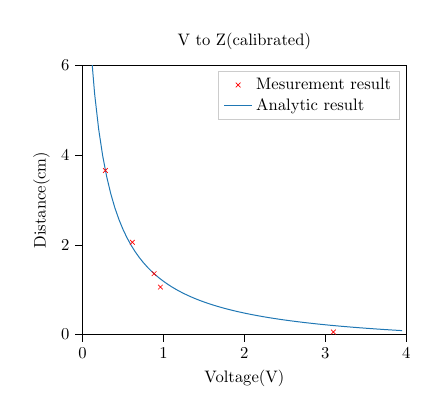
\begin{tikzpicture}[scale=0.6]

    \definecolor{darkgray176}{RGB}{176,176,176}
    \definecolor{lightgray204}{RGB}{204,204,204}
    \definecolor{steelblue31119180}{RGB}{31,119,180}

    \begin{axis}[
            legend cell align={left},
            legend style={fill opacity=0.8, draw opacity=1, text opacity=1, draw=lightgray204},
            tick align=outside,
            tick pos=left,
            title={V to Z(calibrated)},
            x grid style={darkgray176},
            xlabel={Voltage(V)},
            xmin=0, xmax=4,
            xtick style={color=black},
            y grid style={darkgray176},
            ylabel={Distance(cm)},
            ymin=0, ymax=6,
            ytick style={color=black}
        ]
        \addplot [draw=red, fill=red, mark=x, only marks]
        table{%
                x  y
                0.884652981427175 1.36
                0.962854349951124 1.06
                0.6158357771261 2.06
                0.283479960899315 3.66
                3.1 0.06
            };
        \addlegendentry{Mesurement result}
        \addplot [semithick, steelblue31119180]
        table {%
                0.1 6.4641535599316
                0.15 5.37308726287651
                0.2 4.58340934315951
                0.25 3.98539459003494
                0.3 3.51681650683061
                0.35 3.13975518622357
                0.4 2.82978502820009
                0.45 2.57046248026751
                0.5 2.35031173004713
                0.55 2.16108044731913
                0.6 1.99668222972617
                0.65 1.85252976406261
                0.7 1.72510006239472
                0.75 1.61164271051478
                0.8 1.50997909793879
                0.85 1.41836116391551
                0.9 1.33537004518959
                0.95 1.2598420666647
                1 1.19081383924829
                1.05 1.12748094718865
                1.1 1.06916645606743
                1.15 1.01529662163507
                1.2 0.965381949070308
                1.25 0.91900227643828
                1.3 0.875794918970355
                1.35 0.835445165648643
                1.4 0.797678601014675
                1.45 0.76225485591001
                1.5 0.728962486232905
                1.55 0.697614749102112
                1.6 0.668046098170044
                1.65 0.64010925917783
                1.7 0.613672776685022
                1.75 0.588618945723909
                1.8 0.564842059712537
                1.85 0.542246919611502
                1.9 0.520747559981895
                1.95 0.500266155999734
                2 0.4807320821326
                2.05 0.462081098481418
                2.1 0.44425464503382
                2.15 0.427199227493099
                2.2 0.410865881113218
                2.25 0.395209701220615
                2.3 0.380189430942645
                2.35 0.365767098172001
                2.4 0.351907695040933
                2.45 0.338578894209127
                2.5 0.325750797124968
                2.55 0.313395710133886
                2.6 0.301487944905011
                2.65 0.290003640149328
                2.7 0.278920602025577
                2.75 0.268218160987767
                2.8 0.257877043131538
                2.85 0.247879254354565
                2.9 0.238207975866317
                2.95 0.228847469770748
                3 0.219782993606939
                3.05 0.211000722871594
                3.1 0.20248768066697
                3.15 0.194231673721241
                3.2 0.186221234117925
                3.25 0.17844556614871
                3.3 0.170894497771755
                3.35 0.16355843621646
                3.4 0.156428327327304
                3.45 0.14949561828442
                3.5 0.142752223378187
                3.55 0.136190492549872
                3.6 0.129803182440976
                3.65 0.123583429720971
                3.7 0.117524726486916
                3.75 0.111620897549604
                3.8 0.105866079439582
                3.85 0.100254700983005
                3.9 0.0947814653120588
                3.95 0.0894413331878457
            };
        \addlegendentry{Analytic result}
    \end{axis}

\end{tikzpicture}

    \caption{Calibration result}
\end{figure}

\section{Fitting the trace}
\begin{figure}[htbp]
    \centering
    % This file was created with tikzplotlib v0.10.1.
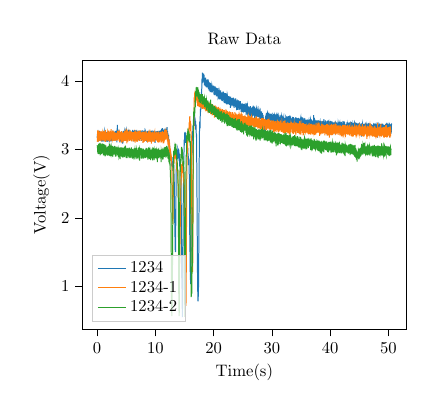
\begin{tikzpicture}[scale=0.6]

    \definecolor{darkgray176}{RGB}{176,176,176}
    \definecolor{darkorange25512714}{RGB}{255,127,14}
    \definecolor{forestgreen4416044}{RGB}{44,160,44}
    \definecolor{lightgray204}{RGB}{204,204,204}
    \definecolor{steelblue31119180}{RGB}{31,119,180}

    \begin{axis}[
            legend cell align={left},
            legend style={
                    fill opacity=0.8,
                    draw opacity=1,
                    text opacity=1,
                    at={(0.03,0.03)},
                    anchor=south west,
                    draw=lightgray204
                },
            tick align=outside,
            tick pos=left,
            title={Raw Data},
            x grid style={darkgray176},
            xlabel={Time(s)},
            xmin=-2.50165, xmax=53.06265,
            xtick style={color=black},
            y grid style={darkgray176},
            ylabel={Voltage(V)},
            ymin=0.373900293255132, ymax=4.29863147605083,
            ytick style={color=black}
        ]
        \addplot [semithick, steelblue31119180]
        table {%
                0.024 3.17204301075269
                0.063 3.2258064516129
                0.095 3.19159335288368
                0.128 3.17693059628543
                0.16 3.25024437927664
                0.192 3.11339198435973
                0.225 3.22091886608016
                0.258 3.20625610948192
                0.29 3.13294232649071
                0.323 3.25024437927664
                0.356 3.19159335288368
                0.388 3.14271749755621
                0.42 3.26979472140762
                0.453 3.13782991202346
                0.485 3.19159335288368
                0.518 3.24046920821114
                0.55 3.13294232649071
                0.583 3.24046920821114
                0.615 3.22091886608016
                0.648 3.13294232649071
                0.679 3.26001955034213
                0.712 3.16226783968719
                0.745 3.16715542521994
                0.777 3.24535679374389
                0.809 3.11339198435973
                0.842 3.2258064516129
                0.874 3.2258064516129
                0.907 3.11827956989247
                0.939 3.2258064516129
                0.971 3.15738025415445
                1.004 3.17693059628543
                1.036 3.26001955034213
                1.069 3.12805474095797
                1.101 3.23069403714565
                1.133 3.24046920821114
                1.166 3.11339198435973
                1.199 3.25024437927664
                1.231 3.26490713587488
                1.263 3.17693059628543
                1.297 3.25024437927664
                1.329 3.17204301075269
                1.361 3.16715542521994
                1.394 3.24046920821114
                1.426 3.13294232649071
                1.459 3.24046920821114
                1.491 3.23069403714565
                1.523 3.12805474095797
                1.556 3.25513196480938
                1.589 3.17693059628543
                1.62 3.15738025415445
                1.653 3.25513196480938
                1.686 3.10850439882698
                1.718 3.21603128054741
                1.751 3.2258064516129
                1.783 3.11339198435973
                1.818 3.2258064516129
                1.851 3.25024437927664
                1.884 3.12316715542522
                1.915 3.24535679374389
                1.948 3.19159335288368
                1.981 3.11827956989247
                2.014 3.2258064516129
                2.046 3.17204301075269
                2.078 3.15738025415445
                2.111 3.24046920821114
                2.144 3.1524926686217
                2.177 3.19159335288368
                2.209 3.23069403714565
                2.241 3.11827956989247
                2.275 3.2258064516129
                2.308 3.24535679374389
                2.34 3.11827956989247
                2.373 3.25513196480938
                2.405 3.17693059628543
                2.438 3.11827956989247
                2.47 3.24535679374389
                2.503 3.14760508308895
                2.536 3.20136852394917
                2.568 3.23069403714565
                2.6 3.14271749755621
                2.633 3.21603128054741
                2.666 3.21114369501466
                2.699 3.12316715542522
                2.731 3.27468230694037
                2.763 3.18670576735093
                2.796 3.13294232649071
                2.829 3.24046920821114
                2.862 3.14760508308895
                2.893 3.20136852394917
                2.926 3.25024437927664
                2.959 3.14760508308895
                2.992 3.24046920821114
                3.024 3.2355816226784
                3.057 3.13294232649071
                3.089 3.24046920821114
                3.122 3.21114369501466
                3.154 3.13294232649071
                3.187 3.26490713587488
                3.22 3.1524926686217
                3.252 3.19159335288368
                3.286 3.27468230694037
                3.318 3.1524926686217
                3.351 3.2355816226784
                3.384 3.2355816226784
                3.416 3.10361681329423
                3.448 3.25024437927664
                3.484 3.35777126099707
                3.516 3.19648093841642
                3.549 3.29912023460411
                3.581 3.25024437927664
                3.614 3.1524926686217
                3.647 3.26001955034213
                3.679 3.22091886608016
                3.712 3.17204301075269
                3.744 3.27468230694037
                3.777 3.17204301075269
                3.81 3.21114369501466
                3.842 3.27468230694037
                3.874 3.10361681329423
                3.907 3.24046920821114
                3.94 3.22091886608016
                3.973 3.10361681329423
                4.004 3.2355816226784
                4.037 3.19159335288368
                4.07 3.13782991202346
                4.103 3.21603128054741
                4.135 3.12316715542522
                4.168 3.19159335288368
                4.2 3.24046920821114
                4.233 3.11339198435973
                4.265 3.21114369501466
                4.299 3.2355816226784
                4.331 3.08406647116325
                4.364 3.20136852394917
                4.397 3.19648093841642
                4.429 3.08895405669599
                4.462 3.26490713587488
                4.494 3.14760508308895
                4.527 3.16715542521994
                4.559 3.2355816226784
                4.592 3.12805474095797
                4.625 3.24046920821114
                4.658 3.25513196480938
                4.689 3.13782991202346
                4.722 3.25513196480938
                4.755 3.2355816226784
                4.788 3.13782991202346
                4.82 3.26001955034213
                4.852 3.20136852394917
                4.885 3.17204301075269
                4.918 3.28445747800587
                4.951 3.14271749755621
                4.983 3.26001955034213
                5.015 3.25024437927664
                5.048 3.12805474095797
                5.081 3.26490713587488
                5.113 3.25024437927664
                5.148 3.1524926686217
                5.181 3.25513196480938
                5.214 3.25024437927664
                5.246 3.14271749755621
                5.279 3.26001955034213
                5.312 3.2355816226784
                5.345 3.1524926686217
                5.378 3.28934506353861
                5.41 3.18181818181818
                5.442 3.19159335288368
                5.475 3.26979472140762
                5.508 3.16226783968719
                5.54 3.26001955034213
                5.572 3.26490713587488
                5.605 3.12316715542522
                5.638 3.28445747800587
                5.67 3.2258064516129
                5.703 3.14760508308895
                5.736 3.26979472140762
                5.768 3.20625610948192
                5.8 3.18670576735093
                5.833 3.26001955034213
                5.866 3.14271749755621
                5.898 3.23069403714565
                5.931 3.25024437927664
                5.963 3.14760508308895
                5.996 3.26001955034213
                6.029 3.20625610948192
                6.061 3.15738025415445
                6.093 3.28445747800587
                6.126 3.17204301075269
                6.159 3.21603128054741
                6.192 3.27468230694037
                6.224 3.11827956989247
                6.256 3.25024437927664
                6.29 3.26979472140762
                6.323 3.12805474095797
                6.355 3.24046920821114
                6.388 3.2355816226784
                6.42 3.14271749755621
                6.453 3.27956989247312
                6.486 3.19159335288368
                6.518 3.18181818181818
                6.55 3.24046920821114
                6.583 3.16226783968719
                6.616 3.18670576735093
                6.648 3.26001955034213
                6.681 3.12805474095797
                6.714 3.28445747800587
                6.746 3.24046920821114
                6.778 3.17204301075269
                6.811 3.26979472140762
                6.846 3.22091886608016
                6.879 3.13782991202346
                6.912 3.25024437927664
                6.944 3.14760508308895
                6.976 3.17693059628543
                7.009 3.26001955034213
                7.042 3.16226783968719
                7.074 3.21114369501466
                7.107 3.27468230694037
                7.139 3.13782991202346
                7.172 3.24535679374389
                7.204 3.25024437927664
                7.237 3.12805474095797
                7.27 3.26979472140762
                7.303 3.2258064516129
                7.335 3.1524926686217
                7.368 3.26001955034213
                7.401 3.18670576735093
                7.434 3.18670576735093
                7.465 3.26490713587488
                7.498 3.1524926686217
                7.531 3.23069403714565
                7.564 3.2355816226784
                7.596 3.12316715542522
                7.628 3.24535679374389
                7.661 3.21603128054741
                7.694 3.14760508308895
                7.727 3.27956989247312
                7.758 3.17204301075269
                7.791 3.19648093841642
                7.824 3.26001955034213
                7.857 3.15738025415445
                7.889 3.22091886608016
                7.921 3.25024437927664
                7.954 3.11827956989247
                7.987 3.26979472140762
                8.019 3.21114369501466
                8.052 3.13782991202346
                8.084 3.27468230694037
                8.117 3.17204301075269
                8.15 3.20625610948192
                8.182 3.26979472140762
                8.215 3.12805474095797
                8.247 3.24535679374389
                8.28 3.23069403714565
                8.313 3.12316715542522
                8.346 3.24046920821114
                8.379 3.2258064516129
                8.411 3.14760508308895
                8.443 3.26001955034213
                8.476 3.20625610948192
                8.511 3.11339198435973
                8.544 3.26001955034213
                8.577 3.20136852394917
                8.609 3.16715542521994
                8.641 3.26979472140762
                8.674 3.15738025415445
                8.707 3.20625610948192
                8.739 3.26001955034213
                8.772 3.12316715542522
                8.805 3.23069403714565
                8.837 3.24046920821114
                8.869 3.12805474095797
                8.902 3.26001955034213
                8.935 3.20136852394917
                8.968 3.15738025415445
                8.999 3.26001955034213
                9.032 3.17204301075269
                9.065 3.20625610948192
                9.098 3.26490713587488
                9.131 3.14760508308895
                9.162 3.24046920821114
                9.195 3.2355816226784
                9.228 3.11339198435973
                9.261 3.27468230694037
                9.294 3.2258064516129
                9.327 3.12805474095797
                9.36 3.26979472140762
                9.392 3.21114369501466
                9.424 3.17693059628543
                9.457 3.26001955034213
                9.49 3.15738025415445
                9.522 3.24535679374389
                9.554 3.25024437927664
                9.587 3.12316715542522
                9.62 3.2355816226784
                9.653 3.2258064516129
                9.686 3.14271749755621
                9.717 3.26490713587488
                9.75 3.19648093841642
                9.783 3.14271749755621
                9.816 3.26979472140762
                9.848 3.14760508308895
                9.881 3.23069403714565
                9.913 3.26979472140762
                9.946 3.09384164222874
                9.978 3.23069403714565
                10.011 3.22091886608016
                10.044 3.13782991202346
                10.076 3.26001955034213
                10.108 3.20625610948192
                10.141 3.14271749755621
                10.177 3.25024437927664
                10.209 3.2258064516129
                10.242 3.17693059628543
                10.274 3.26490713587488
                10.308 3.19648093841642
                10.341 3.17204301075269
                10.374 3.25024437927664
                10.405 3.14271749755621
                10.438 3.17204301075269
                10.471 3.26490713587488
                10.504 3.13294232649071
                10.536 3.25024437927664
                10.569 3.24535679374389
                10.601 3.13782991202346
                10.634 3.24535679374389
                10.667 3.20136852394917
                10.699 3.15738025415445
                10.732 3.26979472140762
                10.765 3.16226783968719
                10.797 3.19159335288368
                10.829 3.27468230694037
                10.862 3.13294232649071
                10.895 3.24535679374389
                10.928 3.25024437927664
                10.96 3.13294232649071
                10.993 3.28445747800587
                11.025 3.24046920821114
                11.058 3.17204301075269
                11.09 3.29423264907136
                11.123 3.20136852394917
                11.156 3.23069403714565
                11.189 3.3088954056696
                11.22 3.18181818181818
                11.253 3.26490713587488
                11.286 3.29423264907136
                11.32 3.1524926686217
                11.353 3.26490713587488
                11.385 3.25513196480938
                11.417 3.17693059628543
                11.45 3.28445747800587
                11.483 3.22091886608016
                11.515 3.18670576735093
                11.548 3.27468230694037
                11.581 3.19159335288368
                11.613 3.2355816226784
                11.645 3.30400782013685
                11.681 3.23069403714565
                11.713 3.2258064516129
                11.746 3.29912023460411
                11.779 3.18181818181818
                11.81 3.27468230694037
                11.843 3.29423264907136
                11.876 3.17204301075269
                11.909 3.29912023460411
                11.94 3.2355816226784
                11.973 3.22091886608016
                12.006 3.32355816226784
                12.038 3.20625610948192
                12.07 3.26001955034213
                12.103 3.26001955034213
                12.135 3.14271749755621
                12.168 3.2355816226784
                12.2 3.15738025415445
                12.233 3.09872922776149
                12.265 3.21114369501466
                12.299 3.09872922776149
                12.332 3.03030303030303
                12.363 3.14760508308895
                12.396 2.94721407624633
                12.429 3.02541544477028
                12.462 3.05962854349951
                12.493 2.91788856304985
                12.526 3.0058651026393
                12.559 2.95698924731183
                12.591 2.88367546432063
                12.623 2.96676441837732
                12.656 2.86412512218964
                12.688 2.86901270772239
                12.721 2.90811339198436
                12.753 2.76148582600196
                12.786 2.86412512218964
                12.818 2.81036168132942
                12.851 2.75171065493646
                12.883 2.88856304985337
                12.915 2.78103616813294
                12.948 2.74193548387097
                12.981 2.82502443792766
                13.014 2.68817204301075
                13.045 2.79569892473118
                13.078 2.81524926686217
                13.111 2.6930596285435
                13.143 2.81036168132942
                13.175 2.74682306940371
                13.21 2.62952101661779
                13.243 2.57575757575758
                13.276 2.31182795698925
                13.308 1.95503421309873
                13.341 1.95992179863148
                13.374 1.74486803519062
                13.407 1.544477028348
                13.438 1.52492668621701
                13.471 1.50048875855327
                13.504 1.85728250244379
                13.537 2.2238514173998
                13.569 2.47311827956989
                13.601 2.80058651026393
                13.634 2.81524926686217
                13.666 2.78103616813294
                13.699 2.96676441837732
                13.731 2.85923753665689
                13.763 2.94232649071359
                13.796 2.99120234604106
                13.829 2.85923753665689
                13.861 3.00097751710655
                13.893 2.98631476050831
                13.926 2.87390029325513
                13.959 3.01075268817204
                13.99 2.93743890518084
                14.023 2.90322580645161
                14.056 2.9960899315738
                14.089 2.82991202346041
                14.12 2.93255131964809
                14.153 2.87878787878788
                14.186 2.75171065493646
                14.218 2.85434995112414
                14.251 2.73704789833822
                14.283 2.67839687194526
                14.316 2.80058651026393
                14.349 2.70772238514174
                14.382 2.70283479960899
                14.414 2.72238514173998
                14.446 2.23851417399804
                14.479 1.88172043010753
                14.512 1.44672531769306
                14.543 1.02150537634409
                14.576 0.987292277614858
                14.609 0.752688172043011
                14.642 0.552297165200391
                14.673 0.718475073313783
                14.709 0.957966764418377
                14.742 1.41251221896383
                14.774 2.05767350928641
                14.807 2.33137829912023
                14.839 2.52199413489736
                14.872 2.77126099706745
                14.905 2.81524926686217
                14.938 3.08895405669599
                14.969 3.14760508308895
                15.002 3.05962854349951
                15.035 3.24535679374389
                15.068 3.19159335288368
                15.1 3.12316715542522
                15.133 3.25513196480938
                15.165 3.13294232649071
                15.198 3.16715542521994
                15.23 3.20625610948192
                15.263 3.09384164222874
                15.296 3.19648093841642
                15.33 3.1524926686217
                15.362 3.06451612903226
                15.394 3.14760508308895
                15.427 3.11827956989247
                15.46 2.97165200391007
                15.493 3.10850439882698
                15.525 3.00097751710655
                15.558 2.94721407624633
                15.591 3.02052785923754
                15.623 2.87878787878788
                15.655 2.8494623655914
                15.688 2.90322580645161
                15.721 2.77126099706745
                15.754 2.80547409579668
                15.787 2.81524926686217
                15.818 2.64418377321603
                15.851 2.6099706744868
                15.884 2.14076246334311
                15.917 1.62267839687195
                15.949 1.52492668621701
                15.982 1.27077223851417
                16.015 1.11436950146628
                16.048 1.08993157380254
                16.079 1.03616813294233
                16.112 1.32942326490714
                16.145 1.83773216031281
                16.178 2.27272727272727
                16.21 2.7761485826002
                16.246 2.96187683284457
                16.278 2.91788856304985
                16.316 2.98631476050831
                16.349 3.19648093841642
                16.381 3.26490713587488
                16.414 3.18181818181818
                16.447 3.34799608993157
                16.48 3.26490713587488
                16.513 3.31378299120235
                16.544 3.43597262952102
                16.577 3.34310850439883
                16.61 3.46041055718475
                16.643 3.50928641251222
                16.675 3.35777126099707
                16.708 3.47996089931574
                16.741 3.48484848484848
                16.774 3.33822091886608
                16.805 3.4652981427175
                16.838 3.36265884652981
                16.871 3.35777126099707
                16.904 3.41642228739003
                16.936 3.28934506353861
                16.969 3.33822091886608
                17.002 3.36265884652981
                17.035 3.17693059628543
                17.067 3.2258064516129
                17.099 2.95210166177908
                17.132 2.52688172043011
                17.165 2.16520039100684
                17.198 1.71065493646139
                17.23 1.24633431085044
                17.263 1.07038123167155
                17.296 0.811339198435973
                17.329 0.782013685239492
                17.361 0.879765395894428
                17.394 0.850439882697947
                17.427 1.11436950146628
                17.46 1.57869012707722
                17.492 1.98924731182796
                17.524 2.63440860215054
                17.557 3.16226783968719
                17.59 3.29912023460411
                17.623 3.40664711632454
                17.655 3.33822091886608
                17.688 3.33333333333333
                17.721 3.54838709677419
                17.756 3.59237536656891
                17.788 3.54349951124145
                17.821 3.68035190615836
                17.853 3.59726295210166
                17.886 3.71456500488759
                17.918 3.83675464320626
                17.951 3.80254154447703
                17.984 3.95894428152493
                18.017 4.03714565004888
                18.049 3.96383186705767
                18.081 4.12023460410557
                18.114 4.07624633431085
                18.147 3.97360703812317
                18.18 4.11045943304008
                18.212 4.01759530791789
                18.244 4.02248289345064
                18.277 4.10557184750733
                18.31 3.98826979472141
                18.343 4.02737047898338
                18.376 4.08602150537634
                18.409 3.93450635386119
                18.441 4.02737047898338
                18.473 4.01759530791789
                18.506 3.93450635386119
                18.539 4.04203323558162
                18.572 3.98338220918866
                18.605 3.91984359726295
                18.636 4.04692082111437
                18.669 3.92961876832845
                18.702 3.97360703812317
                18.735 4.01759530791789
                18.767 3.90518084066471
                18.8 4.01759530791789
                18.832 3.99315738025415
                18.865 3.91006842619746
                18.897 3.98826979472141
                18.93 3.93939393939394
                18.963 3.98338220918866
                18.995 4.02248289345064
                19.027 3.90029325513196
                19.06 3.93939393939394
                19.093 3.98826979472141
                19.126 3.88074291300098
                19.159 3.97849462365591
                19.19 3.96871945259042
                19.223 3.85630498533724
                19.256 3.97849462365591
                19.291 3.94428152492669
                19.324 3.87585532746823
                19.357 3.95894428152493
                19.39 3.93939393939394
                19.423 3.83675464320626
                19.456 3.96871945259042
                19.487 3.91006842619746
                19.52 3.86119257086999
                19.553 3.94428152492669
                19.586 3.83675464320626
                19.618 3.90029325513196
                19.65 3.94428152492669
                19.683 3.83186705767351
                19.716 3.93450635386119
                19.748 3.91984359726295
                19.781 3.83186705767351
                19.814 3.92961876832845
                19.846 3.88074291300098
                19.878 3.85630498533724
                19.911 3.91495601173021
                19.944 3.87585532746823
                19.977 3.88074291300098
                20.008 3.92961876832845
                20.041 3.80254154447703
                20.074 3.89051808406647
                20.107 3.89540566959922
                20.14 3.79276637341153
                20.172 3.90518084066471
                20.205 3.86119257086999
                20.237 3.81231671554252
                20.27 3.91984359726295
                20.302 3.81231671554252
                20.336 3.81720430107527
                20.369 3.90518084066471
                20.401 3.79765395894428
                20.433 3.86608015640274
                20.466 3.87096774193548
                20.499 3.77321603128055
                20.532 3.88074291300098
                20.564 3.84652981427175
                20.596 3.77321603128055
                20.629 3.88563049853372
                20.662 3.80254154447703
                20.695 3.82209188660802
                20.727 3.89540566959922
                20.76 3.75855327468231
                20.795 3.7683284457478
                20.828 3.86608015640274
                20.86 3.77810361681329
                20.892 3.80742913000978
                20.925 3.86119257086999
                20.958 3.72922776148583
                20.99 3.84652981427175
                21.023 3.83186705767351
                21.056 3.72922776148583
                21.088 3.841642228739
                21.121 3.80742913000978
                21.153 3.76344086021505
                21.186 3.86119257086999
                21.219 3.7683284457478
                21.252 3.80742913000978
                21.284 3.83186705767351
                21.316 3.72434017595308
                21.35 3.80254154447703
                21.383 3.83186705767351
                21.415 3.70967741935484
                21.448 3.83186705767351
                21.481 3.79276637341153
                21.513 3.70478983382209
                21.545 3.81720430107527
                21.578 3.77321603128055
                21.611 3.72922776148583
                21.644 3.84652981427175
                21.677 3.71945259042033
                21.708 3.7683284457478
                21.741 3.82697947214076
                21.774 3.69012707722385
                21.807 3.81231671554252
                21.839 3.80742913000978
                21.872 3.67546432062561
                21.904 3.79765395894428
                21.937 3.73900293255132
                21.969 3.73900293255132
                22.002 3.82209188660802
                22.035 3.6950146627566
                22.068 3.74877810361681
                22.099 3.81231671554252
                22.132 3.66568914956012
                22.165 3.77321603128055
                22.198 3.7683284457478
                22.231 3.65591397849462
                22.263 3.81720430107527
                22.296 3.72434017595308
                22.332 3.65591397849462
                22.365 3.78787878787879
                22.397 3.77321603128055
                22.43 3.66080156402737
                22.462 3.77321603128055
                22.495 3.70478983382209
                22.528 3.67546432062561
                22.56 3.77810361681329
                22.593 3.6852394916911
                22.626 3.69012707722385
                22.658 3.7683284457478
                22.69 3.65102639296188
                22.723 3.75855327468231
                22.756 3.75366568914956
                22.789 3.65102639296188
                22.821 3.74877810361681
                22.854 3.72434017595308
                22.887 3.60703812316716
                22.919 3.7683284457478
                22.951 3.6950146627566
                22.984 3.6852394916911
                23.017 3.74877810361681
                23.05 3.67546432062561
                23.083 3.72434017595308
                23.114 3.72922776148583
                23.147 3.62658846529814
                23.18 3.72434017595308
                23.213 3.74877810361681
                23.245 3.64613880742913
                23.278 3.74389051808407
                23.31 3.66568914956012
                23.344 3.64613880742913
                23.376 3.75366568914956
                23.409 3.63636363636364
                23.442 3.69012707722385
                23.475 3.71945259042033
                23.506 3.60703812316716
                23.539 3.70967741935484
                23.572 3.69990224828934
                23.605 3.63147605083089
                23.638 3.72434017595308
                23.67 3.67057673509286
                23.703 3.63636363636364
                23.735 3.74389051808407
                23.768 3.6217008797654
                23.8 3.67057673509286
                23.833 3.73900293255132
                23.864 3.60703812316716
                23.896 3.70967741935484
                23.928 3.62658846529814
                23.961 3.64125122189638
                23.993 3.71456500488759
                24.026 3.57771260997067
                24.058 3.69990224828934
                24.09 3.70478983382209
                24.123 3.57771260997067
                24.156 3.69990224828934
                24.188 3.63636363636364
                24.22 3.59726295210166
                24.253 3.71456500488759
                24.286 3.60215053763441
                24.318 3.64613880742913
                24.351 3.69012707722385
                24.384 3.57282502443793
                24.417 3.69012707722385
                24.449 3.6852394916911
                24.481 3.58260019550342
                24.514 3.69990224828934
                24.546 3.6217008797654
                24.579 3.58748778103617
                24.611 3.70478983382209
                24.644 3.58748778103617
                24.676 3.64125122189638
                24.709 3.66568914956012
                24.741 3.54838709677419
                24.773 3.66568914956012
                24.806 3.6217008797654
                24.839 3.56793743890518
                24.871 3.65102639296188
                24.903 3.58260019550342
                24.936 3.59726295210166
                24.969 3.66080156402737
                25 3.54838709677419
                25.033 3.65102639296188
                25.066 3.64613880742913
                25.099 3.54349951124145
                25.131 3.66568914956012
                25.163 3.57282502443793
                25.196 3.58260019550342
                25.228 3.65102639296188
                25.261 3.54349951124145
                25.293 3.63147605083089
                25.326 3.64613880742913
                25.369 3.63636363636364
                25.404 3.6217008797654
                25.439 3.54349951124145
                25.474 3.59237536656891
                25.508 3.62658846529814
                25.542 3.6119257086999
                25.577 3.49951124144673
                25.612 3.60703812316716
                25.647 3.67057673509286
                25.681 3.57771260997067
                25.715 3.52883675464321
                25.75 3.62658846529814
                25.785 3.64125122189638
                25.82 3.51906158357771
                25.854 3.52883675464321
                25.889 3.6217008797654
                25.924 3.6217008797654
                25.958 3.51417399804497
                25.993 3.54349951124145
                26.028 3.62658846529814
                26.062 3.58748778103617
                26.097 3.49951124144673
                26.131 3.54838709677419
                26.166 3.6119257086999
                26.201 3.58260019550342
                26.235 3.48973607038123
                26.27 3.56793743890518
                26.304 3.63147605083089
                26.339 3.55816226783969
                26.374 3.47996089931574
                26.409 3.56304985337243
                26.444 3.60215053763441
                26.478 3.55327468230694
                26.513 3.48973607038123
                26.548 3.56304985337243
                26.583 3.6119257086999
                26.617 3.52394916911046
                26.651 3.47996089931574
                26.686 3.60215053763441
                26.721 3.59726295210166
                26.756 3.54349951124145
                26.79 3.49951124144673
                26.824 3.59726295210166
                26.859 3.58748778103617
                26.894 3.50928641251222
                26.929 3.48973607038123
                26.963 3.61681329423265
                27 3.6119257086999
                27.035 3.52394916911046
                27.07 3.44574780058651
                27.105 3.54349951124145
                27.14 3.59726295210166
                27.174 3.49462365591398
                27.209 3.53372434017595
                27.244 3.57282502443793
                27.279 3.58748778103617
                27.314 3.48973607038123
                27.347 3.47507331378299
                27.382 3.58260019550342
                27.417 3.59237536656891
                27.453 3.50928641251222
                27.488 3.47996089931574
                27.523 3.56793743890518
                27.557 3.57282502443793
                27.592 3.50439882697947
                27.627 3.47018572825024
                27.662 3.55816226783969
                27.697 3.56304985337243
                27.731 3.47996089931574
                27.766 3.47996089931574
                27.8 3.57282502443793
                27.835 3.55816226783969
                27.87 3.47018572825024
                27.905 3.455522971652
                27.939 3.55327468230694
                27.974 3.56304985337243
                28.009 3.44574780058651
                28.044 3.4652981427175
                28.079 3.54838709677419
                28.113 3.52883675464321
                28.148 3.455522971652
                28.183 3.47996089931574
                28.218 3.55327468230694
                28.253 3.51906158357771
                28.288 3.43597262952102
                28.322 3.47996089931574
                28.357 3.52883675464321
                28.392 3.49951124144673
                28.427 3.38709677419355
                28.461 3.47996089931574
                28.495 3.50439882697947
                28.531 3.455522971652
                28.566 3.31867057673509
                28.604 3.26001955034213
                28.639 3.3822091886608
                28.674 3.36265884652981
                28.708 3.26490713587488
                28.742 3.20625610948192
                28.777 3.3088954056696
                28.812 3.33333333333333
                28.847 3.31867057673509
                28.881 3.43597262952102
                28.916 3.47507331378299
                28.951 3.48484848484848
                28.986 3.3822091886608
                29.021 3.3919843597263
                29.056 3.53372434017595
                29.09 3.47507331378299
                29.125 3.41153470185728
                29.16 3.41642228739003
                29.195 3.51906158357771
                29.23 3.52883675464321
                29.264 3.38709677419355
                29.299 3.43597262952102
                29.334 3.51417399804497
                29.369 3.49951124144673
                29.403 3.41153470185728
                29.437 3.43597262952102
                29.472 3.53372434017595
                29.507 3.51417399804497
                29.542 3.40175953079179
                29.577 3.44574780058651
                29.613 3.51906158357771
                29.647 3.48973607038123
                29.682 3.40664711632454
                29.717 3.43597262952102
                29.752 3.49951124144673
                29.787 3.50439882697947
                29.821 3.41153470185728
                29.856 3.43108504398827
                29.891 3.51906158357771
                29.925 3.48484848484848
                29.96 3.39687194525904
                29.995 3.46041055718475
                30.029 3.49951124144673
                30.064 3.47507331378299
                30.099 3.36265884652981
                30.134 3.45063538611926
                30.169 3.49951124144673
                30.203 3.48973607038123
                30.241 3.42130987292278
                30.275 3.39687194525904
                30.31 3.50928641251222
                30.345 3.50928641251222
                30.38 3.3919843597263
                30.414 3.40664711632454
                30.449 3.50439882697947
                30.484 3.49462365591398
                30.519 3.36754643206256
                30.554 3.3919843597263
                30.588 3.50928641251222
                30.623 3.47018572825024
                30.658 3.40175953079179
                30.693 3.41153470185728
                30.728 3.50928641251222
                30.763 3.47018572825024
                30.797 3.35777126099707
                30.832 3.38709677419355
                30.867 3.48484848484848
                30.902 3.47018572825024
                30.937 3.36265884652981
                30.971 3.39687194525904
                31.006 3.47996089931574
                31.041 3.4652981427175
                31.076 3.35288367546432
                31.111 3.41642228739003
                31.144 3.47018572825024
                31.179 3.45063538611926
                31.214 3.35288367546432
                31.249 3.41153470185728
                31.284 3.47507331378299
                31.319 3.42619745845552
                31.353 3.32844574780059
                31.388 3.47018572825024
                31.423 3.50439882697947
                31.458 3.41642228739003
                31.493 3.36754643206256
                31.527 3.43597262952102
                31.562 3.47996089931574
                31.597 3.40664711632454
                31.631 3.34310850439883
                31.666 3.47996089931574
                31.7 3.4652981427175
                31.736 3.42130987292278
                31.771 3.32844574780059
                31.806 3.43108504398827
                31.843 3.4652981427175
                31.878 3.455522971652
                31.912 3.36754643206256
                31.947 3.34310850439883
                31.982 3.45063538611926
                32.017 3.4652981427175
                32.052 3.35288367546432
                32.087 3.3919843597263
                32.121 3.46041055718475
                32.156 3.43597262952102
                32.191 3.34799608993157
                32.226 3.3919843597263
                32.261 3.46041055718475
                32.294 3.44086021505376
                32.329 3.33822091886608
                32.364 3.41153470185728
                32.399 3.47018572825024
                32.434 3.46041055718475
                32.468 3.33333333333333
                32.503 3.40664711632454
                32.538 3.47996089931574
                32.573 3.3919843597263
                32.608 3.33822091886608
                32.643 3.41642228739003
                32.677 3.47507331378299
                32.712 3.39687194525904
                32.747 3.32844574780059
                32.782 3.455522971652
                32.817 3.48484848484848
                32.851 3.40664711632454
                32.886 3.34310850439883
                32.921 3.44574780058651
                32.956 3.48484848484848
                32.991 3.39687194525904
                33.026 3.32355816226784
                33.06 3.42619745845552
                33.095 3.49462365591398
                33.13 3.39687194525904
                33.165 3.33333333333333
                33.2 3.44574780058651
                33.234 3.47996089931574
                33.269 3.37243401759531
                33.304 3.31867057673509
                33.339 3.41642228739003
                33.378 3.44574780058651
                33.413 3.44574780058651
                33.447 3.36265884652981
                33.485 3.29423264907136
                33.519 3.40175953079179
                33.554 3.47507331378299
                33.589 3.40175953079179
                33.624 3.31378299120235
                33.658 3.40175953079179
                33.693 3.47018572825024
                33.729 3.41153470185728
                33.764 3.32844574780059
                33.798 3.40175953079179
                33.832 3.41642228739003
                33.868 3.41153470185728
                33.903 3.33333333333333
                33.938 3.40175953079179
                33.973 3.46041055718475
                34.008 3.41642228739003
                34.042 3.3088954056696
                34.077 3.37732160312805
                34.112 3.47018572825024
                34.147 3.40664711632454
                34.182 3.31378299120235
                34.216 3.36754643206256
                34.251 3.455522971652
                34.286 3.3919843597263
                34.321 3.32355816226784
                34.356 3.41153470185728
                34.391 3.45063538611926
                34.425 3.40664711632454
                34.46 3.3088954056696
                34.495 3.38709677419355
                34.53 3.46041055718475
                34.565 3.3919843597263
                34.598 3.29423264907136
                34.633 3.38709677419355
                34.668 3.44574780058651
                34.703 3.38709677419355
                34.738 3.31867057673509
                34.772 3.39687194525904
                34.807 3.45063538611926
                34.842 3.3822091886608
                34.877 3.32844574780059
                34.912 3.44574780058651
                34.948 3.46041055718475
                34.982 3.33822091886608
                35.017 3.32355816226784
                35.051 3.42130987292278
                35.089 3.44086021505376
                35.124 3.42619745845552
                35.159 3.31378299120235
                35.193 3.36754643206256
                35.228 3.4652981427175
                35.263 3.39687194525904
                35.298 3.31867057673509
                35.333 3.38709677419355
                35.367 3.43597262952102
                35.402 3.39687194525904
                35.437 3.33822091886608
                35.471 3.36754643206256
                35.506 3.46041055718475
                35.54 3.41642228739003
                35.575 3.29423264907136
                35.61 3.3822091886608
                35.645 3.45063538611926
                35.68 3.40175953079179
                35.715 3.32355816226784
                35.749 3.39687194525904
                35.784 3.43108504398827
                35.819 3.37243401759531
                35.854 3.29912023460411
                35.889 3.39687194525904
                35.923 3.42619745845552
                35.958 3.35288367546432
                35.993 3.28934506353861
                36.028 3.3822091886608
                36.063 3.43597262952102
                36.098 3.37243401759531
                36.132 3.30400782013685
                36.167 3.39687194525904
                36.202 3.43108504398827
                36.237 3.3822091886608
                36.272 3.28934506353861
                36.306 3.40175953079179
                36.341 3.41642228739003
                36.376 3.36754643206256
                36.411 3.3088954056696
                36.446 3.40175953079179
                36.481 3.43597262952102
                36.515 3.33822091886608
                36.55 3.29912023460411
                36.585 3.41642228739003
                36.62 3.43108504398827
                36.655 3.33333333333333
                36.688 3.30400782013685
                36.726 3.34310850439883
                36.761 3.43597262952102
                36.795 3.3822091886608
                36.83 3.28445747800587
                36.865 3.37243401759531
                36.899 3.42130987292278
                36.934 3.37243401759531
                36.969 3.27468230694037
                37.003 3.3919843597263
                37.038 3.41642228739003
                37.073 3.33333333333333
                37.108 3.27468230694037
                37.142 3.40664711632454
                37.177 3.49951124144673
                37.212 3.36754643206256
                37.246 3.26979472140762
                37.281 3.41153470185728
                37.315 3.42130987292278
                37.35 3.32355816226784
                37.385 3.29912023460411
                37.42 3.41153470185728
                37.454 3.40175953079179
                37.489 3.30400782013685
                37.523 3.32844574780059
                37.558 3.42130987292278
                37.593 3.39687194525904
                37.627 3.33333333333333
                37.662 3.34799608993157
                37.697 3.42130987292278
                37.731 3.36265884652981
                37.766 3.27956989247312
                37.8 3.36754643206256
                37.835 3.42130987292278
                37.87 3.34310850439883
                37.904 3.26979472140762
                37.939 3.40175953079179
                37.974 3.3822091886608
                38.008 3.33822091886608
                38.043 3.28445747800587
                38.077 3.40175953079179
                38.112 3.39687194525904
                38.148 3.31867057673509
                38.182 3.28445747800587
                38.216 3.40175953079179
                38.251 3.41153470185728
                38.286 3.30400782013685
                38.323 3.25513196480938
                38.358 3.37732160312805
                38.392 3.41642228739003
                38.427 3.33822091886608
                38.462 3.28445747800587
                38.496 3.3822091886608
                38.531 3.40664711632454
                38.565 3.29912023460411
                38.6 3.29912023460411
                38.635 3.38709677419355
                38.669 3.40664711632454
                38.704 3.31867057673509
                38.738 3.25513196480938
                38.773 3.41642228739003
                38.808 3.3822091886608
                38.843 3.29423264907136
                38.877 3.3088954056696
                38.912 3.44086021505376
                38.946 3.37732160312805
                38.981 3.30400782013685
                39.016 3.35288367546432
                39.05 3.40175953079179
                39.085 3.35288367546432
                39.119 3.26490713587488
                39.154 3.37732160312805
                39.189 3.42130987292278
                39.224 3.37243401759531
                39.259 3.24535679374389
                39.293 3.37732160312805
                39.328 3.41153470185728
                39.363 3.27956989247312
                39.397 3.26490713587488
                39.432 3.38709677419355
                39.467 3.38709677419355
                39.501 3.29912023460411
                39.536 3.28445747800587
                39.57 3.41153470185728
                39.605 3.41153470185728
                39.64 3.27956989247312
                39.674 3.29912023460411
                39.709 3.38709677419355
                39.744 3.39687194525904
                39.778 3.27956989247312
                39.813 3.32355816226784
                39.847 3.40175953079179
                39.882 3.34799608993157
                39.917 3.26979472140762
                39.954 3.27468230694037
                39.989 3.36754643206256
                40.024 3.41642228739003
                40.058 3.28934506353861
                40.093 3.27468230694037
                40.128 3.3919843597263
                40.163 3.38709677419355
                40.198 3.3088954056696
                40.232 3.36265884652981
                40.267 3.3919843597263
                40.302 3.41153470185728
                40.337 3.29912023460411
                40.372 3.23069403714565
                40.407 3.3822091886608
                40.441 3.37732160312805
                40.476 3.31867057673509
                40.511 3.27956989247312
                40.546 3.38709677419355
                40.581 3.38709677419355
                40.615 3.26979472140762
                40.65 3.27468230694037
                40.685 3.3919843597263
                40.72 3.37243401759531
                40.755 3.27956989247312
                40.79 3.26490713587488
                40.824 3.3919843597263
                40.859 3.39687194525904
                40.894 3.27468230694037
                40.929 3.29912023460411
                40.964 3.38709677419355
                40.998 3.3822091886608
                41.032 3.29423264907136
                41.067 3.28445747800587
                41.102 3.3919843597263
                41.137 3.35777126099707
                41.171 3.26001955034213
                41.206 3.3088954056696
                41.241 3.36265884652981
                41.276 3.36754643206256
                41.311 3.26979472140762
                41.346 3.32355816226784
                41.381 3.3919843597263
                41.416 3.37732160312805
                41.451 3.25513196480938
                41.486 3.31867057673509
                41.521 3.37243401759531
                41.555 3.36754643206256
                41.587 3.25024437927664
                41.622 3.38709677419355
                41.657 3.39687194525904
                41.692 3.33822091886608
                41.726 3.22091886608016
                41.761 3.35288367546432
                41.796 3.3919843597263
                41.831 3.29912023460411
                41.866 3.26001955034213
                41.901 3.37732160312805
                41.935 3.40175953079179
                41.97 3.30400782013685
                42.005 3.26490713587488
                42.04 3.37243401759531
                42.075 3.37243401759531
                42.109 3.25513196480938
                42.144 3.23069403714565
                42.179 3.3919843597263
                42.213 3.38709677419355
                42.248 3.32355816226784
                42.283 3.26001955034213
                42.317 3.36754643206256
                42.352 3.41153470185728
                42.387 3.26490713587488
                42.422 3.26001955034213
                42.458 3.3919843597263
                42.492 3.38709677419355
                42.527 3.29423264907136
                42.562 3.26979472140762
                42.597 3.35777126099707
                42.632 3.33333333333333
                42.667 3.29423264907136
                42.701 3.24046920821114
                42.736 3.36265884652981
                42.771 3.36265884652981
                42.805 3.26001955034213
                42.84 3.28445747800587
                42.874 3.37243401759531
                42.909 3.36754643206256
                42.944 3.26001955034213
                42.979 3.26001955034213
                43.014 3.36754643206256
                43.048 3.35288367546432
                43.083 3.26979472140762
                43.118 3.27956989247312
                43.153 3.3822091886608
                43.191 3.3822091886608
                43.226 3.29912023460411
                43.26 3.24046920821114
                43.294 3.35288367546432
                43.329 3.3919843597263
                43.364 3.31378299120235
                43.399 3.26490713587488
                43.433 3.36265884652981
                43.468 3.37243401759531
                43.504 3.28934506353861
                43.539 3.25513196480938
                43.574 3.33822091886608
                43.609 3.39687194525904
                43.643 3.30400782013685
                43.678 3.2355816226784
                43.713 3.37243401759531
                43.747 3.3822091886608
                43.782 3.31378299120235
                43.816 3.26001955034213
                43.851 3.36265884652981
                43.886 3.38709677419355
                43.921 3.27468230694037
                43.956 3.25024437927664
                43.991 3.35288367546432
                44.025 3.38709677419355
                44.06 3.28445747800587
                44.095 3.25513196480938
                44.13 3.37732160312805
                44.165 3.38709677419355
                44.199 3.26979472140762
                44.234 3.22091886608016
                44.268 3.3919843597263
                44.303 3.37243401759531
                44.338 3.25024437927664
                44.372 3.25513196480938
                44.407 3.37243401759531
                44.442 3.36754643206256
                44.477 3.2355816226784
                44.512 3.30400782013685
                44.547 3.38709677419355
                44.582 3.34310850439883
                44.616 3.23069403714565
                44.651 3.28445747800587
                44.686 3.36265884652981
                44.721 3.35777126099707
                44.755 3.24046920821114
                44.79 3.28445747800587
                44.828 3.34799608993157
                44.863 3.37732160312805
                44.898 3.29423264907136
                44.933 3.2355816226784
                44.966 3.35777126099707
                45.001 3.3822091886608
                45.036 3.28445747800587
                45.071 3.25513196480938
                45.106 3.37243401759531
                45.14 3.36754643206256
                45.175 3.29912023460411
                45.21 3.24535679374389
                45.245 3.35777126099707
                45.28 3.35777126099707
                45.315 3.26490713587488
                45.349 3.18670576735093
                45.384 3.36265884652981
                45.419 3.35777126099707
                45.454 3.25513196480938
                45.489 3.26490713587488
                45.522 3.36265884652981
                45.557 3.37732160312805
                45.592 3.26979472140762
                45.627 3.24535679374389
                45.663 3.33822091886608
                45.698 3.34310850439883
                45.732 3.27468230694037
                45.767 3.25024437927664
                45.802 3.36265884652981
                45.837 3.36265884652981
                45.872 3.26979472140762
                45.905 3.27468230694037
                45.94 3.36265884652981
                45.975 3.36754643206256
                46.01 3.26490713587488
                46.045 3.26001955034213
                46.08 3.37732160312805
                46.114 3.34310850439883
                46.149 3.2355816226784
                46.184 3.27956989247312
                46.219 3.35288367546432
                46.254 3.33822091886608
                46.288 3.2355816226784
                46.323 3.29423264907136
                46.358 3.35288367546432
                46.393 3.34799608993157
                46.43 3.28934506353861
                46.465 3.23069403714565
                46.499 3.35777126099707
                46.534 3.38709677419355
                46.569 3.26979472140762
                46.604 3.25513196480938
                46.639 3.34310850439883
                46.673 3.37732160312805
                46.708 3.26979472140762
                46.743 3.23069403714565
                46.778 3.37243401759531
                46.813 3.37243401759531
                46.848 3.26979472140762
                46.882 3.24046920821114
                46.917 3.35288367546432
                46.952 3.34799608993157
                46.987 3.27468230694037
                47.022 3.26490713587488
                47.056 3.34799608993157
                47.091 3.34310850439883
                47.126 3.27956989247312
                47.161 3.25513196480938
                47.196 3.34799608993157
                47.23 3.34310850439883
                47.265 3.25024437927664
                47.299 3.25513196480938
                47.334 3.35777126099707
                47.369 3.33822091886608
                47.404 3.29912023460411
                47.438 3.25513196480938
                47.473 3.36265884652981
                47.508 3.35777126099707
                47.543 3.26979472140762
                47.578 3.28445747800587
                47.612 3.37732160312805
                47.647 3.33333333333333
                47.682 3.25513196480938
                47.717 3.26490713587488
                47.752 3.36754643206256
                47.788 3.33822091886608
                47.821 3.2355816226784
                47.856 3.23069403714565
                47.891 3.34310850439883
                47.926 3.33333333333333
                47.961 3.25024437927664
                47.995 3.27468230694037
                48.03 3.35288367546432
                48.068 3.3919843597263
                48.103 3.29912023460411
                48.138 3.17204301075269
                48.173 3.33333333333333
                48.207 3.35777126099707
                48.242 3.27956989247312
                48.276 3.23069403714565
                48.311 3.33822091886608
                48.346 3.32355816226784
                48.38 3.26979472140762
                48.415 3.24535679374389
                48.45 3.32844574780059
                48.485 3.37243401759531
                48.52 3.27468230694037
                48.555 3.19648093841642
                48.589 3.36265884652981
                48.624 3.35777126099707
                48.659 3.26979472140762
                48.694 3.24046920821114
                48.729 3.33822091886608
                48.763 3.36754643206256
                48.798 3.26490713587488
                48.833 3.25024437927664
                48.868 3.35288367546432
                48.903 3.35777126099707
                48.937 3.27468230694037
                48.972 3.2355816226784
                49.007 3.33822091886608
                49.042 3.37243401759531
                49.077 3.27468230694037
                49.112 3.2355816226784
                49.146 3.32844574780059
                49.181 3.35777126099707
                49.216 3.29423264907136
                49.251 3.24046920821114
                49.286 3.32844574780059
                49.319 3.35288367546432
                49.354 3.25513196480938
                49.389 3.25513196480938
                49.424 3.34799608993157
                49.459 3.35288367546432
                49.494 3.26001955034213
                49.528 3.26979472140762
                49.563 3.34310850439883
                49.598 3.35288367546432
                49.633 3.25024437927664
                49.67 3.2258064516129
                49.704 3.35288367546432
                49.739 3.37732160312805
                49.774 3.28445747800587
                49.809 3.23069403714565
                49.844 3.34310850439883
                49.878 3.35288367546432
                49.913 3.28934506353861
                49.948 3.21603128054741
                49.983 3.36265884652981
                50.017 3.35777126099707
                50.052 3.26001955034213
                50.086 3.21603128054741
                50.121 3.34310850439883
                50.156 3.35288367546432
                50.191 3.24046920821114
                50.225 3.18181818181818
                50.259 3.36754643206256
                50.294 3.33333333333333
                50.329 3.24046920821114
                50.364 3.26979472140762
                50.398 3.33333333333333
                50.433 3.34310850439883
                50.467 3.23069403714565
                50.502 3.26979472140762
                50.537 3.37732160312805
            };
        \addlegendentry{1234}
        \addplot [semithick, darkorange25512714]
        table {%
                0.024 3.11339198435973
                0.063 3.12805474095797
                0.096 3.26979472140762
                0.134 3.26979472140762
                0.165 3.10850439882698
                0.198 3.2355816226784
                0.23 3.24046920821114
                0.263 3.13782991202346
                0.295 3.27468230694037
                0.327 3.16715542521994
                0.36 3.20625610948192
                0.392 3.25513196480938
                0.424 3.12316715542522
                0.456 3.25513196480938
                0.489 3.23069403714565
                0.522 3.13294232649071
                0.553 3.26001955034213
                0.586 3.18670576735093
                0.618 3.21603128054741
                0.651 3.24046920821114
                0.684 3.11827956989247
                0.715 3.26490713587488
                0.748 3.22091886608016
                0.78 3.14760508308895
                0.813 3.25513196480938
                0.844 3.14271749755621
                0.877 3.2258064516129
                0.91 3.25513196480938
                0.942 3.12805474095797
                0.974 3.24046920821114
                1.007 3.2258064516129
                1.039 3.13294232649071
                1.072 3.26490713587488
                1.103 3.14271749755621
                1.137 3.20625610948192
                1.169 3.26490713587488
                1.202 3.12805474095797
                1.234 3.23069403714565
                1.266 3.23069403714565
                1.299 3.11827956989247
                1.331 3.25024437927664
                1.363 3.16715542521994
                1.396 3.19648093841642
                1.428 3.27956989247312
                1.461 3.10850439882698
                1.492 3.21603128054741
                1.525 3.21114369501466
                1.557 3.14271749755621
                1.59 3.24535679374389
                1.623 3.14271749755621
                1.654 3.18670576735093
                1.687 3.24046920821114
                1.719 3.12805474095797
                1.752 3.25513196480938
                1.784 3.21603128054741
                1.819 3.12805474095797
                1.851 3.26001955034213
                1.884 3.25024437927664
                1.916 3.13294232649071
                1.949 3.25513196480938
                1.981 3.19159335288368
                2.014 3.17204301075269
                2.046 3.27468230694037
                2.079 3.12316715542522
                2.112 3.20625610948192
                2.145 3.23069403714565
                2.178 3.11339198435973
                2.209 3.25024437927664
                2.242 3.23069403714565
                2.275 3.13294232649071
                2.308 3.26979472140762
                2.339 3.16715542521994
                2.372 3.16715542521994
                2.405 3.29423264907136
                2.438 3.15738025415445
                2.469 3.2355816226784
                2.502 3.25513196480938
                2.535 3.12316715542522
                2.567 3.26001955034213
                2.599 3.18181818181818
                2.632 3.16715542521994
                2.665 3.27468230694037
                2.697 3.17204301075269
                2.729 3.24046920821114
                2.762 3.27468230694037
                2.794 3.12805474095797
                2.827 3.26001955034213
                2.86 3.20136852394917
                2.892 3.12805474095797
                2.924 3.25513196480938
                2.957 3.14760508308895
                2.99 3.19159335288368
                3.021 3.24046920821114
                3.054 3.12316715542522
                3.087 3.24535679374389
                3.121 3.21603128054741
                3.152 3.12805474095797
                3.185 3.2355816226784
                3.218 3.20136852394917
                3.251 3.12805474095797
                3.282 3.24535679374389
                3.315 3.16715542521994
                3.348 3.19159335288368
                3.38 3.23069403714565
                3.412 3.13294232649071
                3.445 3.22091886608016
                3.48 3.24046920821114
                3.513 3.13782991202346
                3.546 3.27468230694037
                3.577 3.24046920821114
                3.61 3.12805474095797
                3.643 3.24046920821114
                3.676 3.18670576735093
                3.707 3.1524926686217
                3.74 3.26979472140762
                3.773 3.15738025415445
                3.805 3.20136852394917
                3.837 3.25513196480938
                3.87 3.10850439882698
                3.903 3.23069403714565
                3.935 3.21603128054741
                3.968 3.12805474095797
                4 3.25513196480938
                4.033 3.15738025415445
                4.065 3.16715542521994
                4.098 3.25024437927664
                4.131 3.16715542521994
                4.163 3.21114369501466
                4.196 3.26490713587488
                4.229 3.09872922776149
                4.261 3.25024437927664
                4.293 3.18181818181818
                4.326 3.11827956989247
                4.359 3.24535679374389
                4.39 3.15738025415445
                4.423 3.20136852394917
                4.456 3.24535679374389
                4.489 3.10361681329423
                4.52 3.21114369501466
                4.553 3.22091886608016
                4.586 3.13294232649071
                4.618 3.24046920821114
                4.651 3.17204301075269
                4.683 3.13782991202346
                4.716 3.26490713587488
                4.748 3.12316715542522
                4.781 3.2258064516129
                4.813 3.27468230694037
                4.845 3.12316715542522
                4.878 3.25513196480938
                4.911 3.20136852394917
                4.943 3.13782991202346
                4.975 3.30400782013685
                5.008 3.12805474095797
                5.041 3.20625610948192
                5.072 3.28445747800587
                5.105 3.08895405669599
                5.141 3.17693059628543
                5.174 3.26490713587488
                5.207 3.1524926686217
                5.239 3.2258064516129
                5.271 3.24046920821114
                5.304 3.11339198435973
                5.337 3.24046920821114
                5.368 3.2258064516129
                5.401 3.15738025415445
                5.434 3.25024437927664
                5.467 3.1524926686217
                5.498 3.22091886608016
                5.531 3.26979472140762
                5.564 3.12316715542522
                5.596 3.2258064516129
                5.628 3.21114369501466
                5.661 3.13782991202346
                5.694 3.26979472140762
                5.726 3.18670576735093
                5.758 3.18181818181818
                5.791 3.26490713587488
                5.823 3.12805474095797
                5.856 3.25024437927664
                5.889 3.22091886608016
                5.92 3.11827956989247
                5.953 3.25024437927664
                5.986 3.15738025415445
                6.019 3.16226783968719
                6.05 3.24535679374389
                6.083 3.16226783968719
                6.117 3.20136852394917
                6.149 3.25024437927664
                6.181 3.11827956989247
                6.214 3.2355816226784
                6.247 3.21603128054741
                6.279 3.11827956989247
                6.311 3.25024437927664
                6.344 3.15738025415445
                6.376 3.18181818181818
                6.409 3.24046920821114
                6.441 3.11827956989247
                6.473 3.23069403714565
                6.506 3.21603128054741
                6.539 3.09872922776149
                6.572 3.26979472140762
                6.604 3.19648093841642
                6.636 3.13294232649071
                6.669 3.26001955034213
                6.702 3.15738025415445
                6.733 3.19159335288368
                6.766 3.25513196480938
                6.799 3.11827956989247
                6.834 3.21114369501466
                6.866 3.24535679374389
                6.898 3.10850439882698
                6.931 3.24046920821114
                6.964 3.23069403714565
                6.996 3.14760508308895
                7.028 3.24535679374389
                7.061 3.17693059628543
                7.094 3.16715542521994
                7.127 3.26490713587488
                7.159 3.17693059628543
                7.192 3.24535679374389
                7.225 3.26490713587488
                7.257 3.12316715542522
                7.289 3.2355816226784
                7.322 3.21114369501466
                7.354 3.12316715542522
                7.387 3.27956989247312
                7.419 3.16715542521994
                7.452 3.21603128054741
                7.484 3.25024437927664
                7.517 3.16715542521994
                7.549 3.2258064516129
                7.582 3.2258064516129
                7.614 3.12805474095797
                7.647 3.24535679374389
                7.68 3.21603128054741
                7.711 3.14271749755621
                7.744 3.25024437927664
                7.777 3.13782991202346
                7.81 3.21114369501466
                7.841 3.25024437927664
                7.874 3.09384164222874
                7.907 3.26001955034213
                7.939 3.18181818181818
                7.971 3.10361681329423
                8.004 3.25024437927664
                8.036 3.15738025415445
                8.069 3.18670576735093
                8.101 3.26001955034213
                8.135 3.11339198435973
                8.167 3.21114369501466
                8.2 3.24535679374389
                8.232 3.12316715542522
                8.264 3.24046920821114
                8.297 3.18670576735093
                8.33 3.13782991202346
                8.363 3.26490713587488
                8.394 3.12805474095797
                8.427 3.18670576735093
                8.46 3.25024437927664
                8.495 3.13782991202346
                8.527 3.20625610948192
                8.56 3.24535679374389
                8.592 3.11827956989247
                8.625 3.24046920821114
                8.657 3.22091886608016
                8.689 3.09872922776149
                8.722 3.24046920821114
                8.755 3.16226783968719
                8.787 3.19159335288368
                8.819 3.26490713587488
                8.852 3.11827956989247
                8.885 3.21114369501466
                8.916 3.25024437927664
                8.949 3.10850439882698
                8.982 3.21114369501466
                9.015 3.19159335288368
                9.047 3.12805474095797
                9.079 3.28934506353861
                9.113 3.16715542521994
                9.146 3.17693059628543
                9.178 3.24535679374389
                9.21 3.11339198435973
                9.243 3.2355816226784
                9.275 3.23069403714565
                9.308 3.08406647116325
                9.34 3.24535679374389
                9.373 3.19648093841642
                9.405 3.13294232649071
                9.438 3.25513196480938
                9.47 3.13294232649071
                9.502 3.19648093841642
                9.535 3.25024437927664
                9.568 3.10850439882698
                9.601 3.2258064516129
                9.632 3.20136852394917
                9.665 3.13294232649071
                9.698 3.2355816226784
                9.731 3.16715542521994
                9.762 3.17693059628543
                9.795 3.26490713587488
                9.828 3.10850439882698
                9.861 3.2258064516129
                9.892 3.24046920821114
                9.925 3.11827956989247
                9.958 3.24046920821114
                9.991 3.17204301075269
                10.022 3.14271749755621
                10.055 3.24046920821114
                10.088 3.14271749755621
                10.122 3.18181818181818
                10.157 3.25513196480938
                10.189 3.18670576735093
                10.222 3.12805474095797
                10.254 3.26001955034213
                10.287 3.15738025415445
                10.319 3.19159335288368
                10.352 3.24046920821114
                10.384 3.10850439882698
                10.417 3.24046920821114
                10.449 3.22091886608016
                10.482 3.09872922776149
                10.514 3.26001955034213
                10.547 3.16226783968719
                10.579 3.16715542521994
                10.612 3.25513196480938
                10.644 3.10361681329423
                10.677 3.22091886608016
                10.71 3.22091886608016
                10.742 3.11339198435973
                10.774 3.21114369501466
                10.807 3.14271749755621
                10.84 3.14271749755621
                10.872 3.25513196480938
                10.904 3.13782991202346
                10.937 3.19648093841642
                10.97 3.2355816226784
                11.002 3.09872922776149
                11.034 3.25024437927664
                11.067 3.19159335288368
                11.1 3.10850439882698
                11.133 3.2355816226784
                11.165 3.17693059628543
                11.198 3.13294232649071
                11.231 3.26490713587488
                11.264 3.12805474095797
                11.295 3.20136852394917
                11.328 3.24535679374389
                11.361 3.08895405669599
                11.394 3.24535679374389
                11.425 3.23069403714565
                11.458 3.12805474095797
                11.491 3.25513196480938
                11.524 3.19159335288368
                11.555 3.19648093841642
                11.588 3.27956989247312
                11.621 3.1524926686217
                11.656 3.16715542521994
                11.688 3.28934506353861
                11.72 3.1524926686217
                11.753 3.26979472140762
                11.786 3.27956989247312
                11.817 3.14271749755621
                11.85 3.28445747800587
                11.883 3.21603128054741
                11.915 3.20625610948192
                11.948 3.27956989247312
                11.979 3.15738025415445
                12.012 3.25513196480938
                12.045 3.23069403714565
                12.077 3.11827956989247
                12.11 3.21114369501466
                12.143 3.16715542521994
                12.175 3.069403714565
                12.208 3.19648093841642
                12.239 3.05474095796676
                12.272 3.09872922776149
                12.305 3.14760508308895
                12.337 3.0058651026393
                12.369 3.14271749755621
                12.402 3.069403714565
                12.434 2.94721407624633
                12.467 3.09872922776149
                12.498 2.94232649071359
                12.531 2.98631476050831
                12.564 3.01075268817204
                12.596 2.84457478005865
                12.628 2.97653958944282
                12.661 2.9227761485826
                12.693 2.82991202346041
                12.726 2.92766373411535
                12.758 2.83479960899316
                12.79 2.82991202346041
                12.823 2.80547409579668
                12.855 2.51710654936461
                12.888 2.36559139784946
                12.92 2.18963831867058
                12.952 1.97947214076246
                12.985 1.96480938416422
                13.017 1.91104594330401
                13.049 2.04301075268817
                13.082 2.34115347018573
                13.115 2.47311827956989
                13.148 2.7663734115347
                13.182 2.82502443792766
                13.215 2.80547409579668
                13.248 2.89345063538612
                13.28 2.91788856304985
                13.313 2.86412512218964
                13.344 2.9960899315738
                13.377 2.95698924731183
                13.41 2.88856304985337
                13.442 2.97165200391007
                13.474 2.86412512218964
                13.507 2.94721407624633
                13.539 2.98142717497556
                13.572 2.84457478005865
                13.603 2.88367546432063
                13.636 2.7761485826002
                13.669 2.6930596285435
                13.701 2.7761485826002
                13.733 2.66373411534702
                13.766 2.71749755620723
                13.798 2.73704789833822
                13.831 2.6099706744868
                13.862 2.6930596285435
                13.895 2.55131964809384
                13.928 2.46823069403715
                13.96 2.49266862170088
                13.992 2.14076246334311
                14.025 1.88172043010753
                14.057 1.72043010752688
                14.09 1.39784946236559
                14.123 1.48093841642229
                14.155 1.3782991202346
                14.188 1.29032258064516
                14.22 1.55913978494624
                14.253 1.67644183773216
                14.285 1.9208211143695
                14.317 2.29227761485826
                14.35 2.35581622678397
                14.382 2.52688172043011
                14.414 2.56598240469208
                14.447 2.55131964809384
                14.479 2.78103616813294
                14.512 2.76148582600196
                14.544 2.75171065493646
                14.576 2.7663734115347
                14.609 2.65395894428152
                14.641 2.79081133919844
                14.676 2.81036168132942
                14.708 2.70283479960899
                14.741 2.66862170087977
                14.774 2.67350928641251
                14.807 2.53176930596285
                14.838 2.63929618768328
                14.871 2.57086999022483
                14.904 2.50733137829912
                14.937 2.56109481915934
                14.968 2.43890518084066
                15.001 2.48289345063539
                15.034 2.11143695014663
                15.067 1.57869012707722
                15.098 1.33919843597263
                15.132 1.08504398826979
                15.165 0.826001955034213
                15.198 0.821114369501466
                15.229 0.733137829912023
                15.262 0.718475073313783
                15.295 1.06060606060606
                15.328 1.41251221896383
                15.36 2.02834799608993
                15.392 2.56109481915934
                15.425 2.69794721407625
                15.458 2.89345063538612
                15.491 2.96187683284457
                15.522 2.97653958944282
                15.555 3.12805474095797
                15.588 3.10361681329423
                15.621 3.15738025415445
                15.652 3.21114369501466
                15.685 3.17693059628543
                15.718 3.26979472140762
                15.751 3.31867057673509
                15.782 3.2355816226784
                15.815 3.38709677419355
                15.848 3.38709677419355
                15.881 3.33822091886608
                15.912 3.48484848484848
                15.945 3.3822091886608
                15.978 3.36265884652981
                16.011 3.41642228739003
                16.043 3.26979472140762
                16.075 3.37732160312805
                16.108 3.33822091886608
                16.142 3.16715542521994
                16.174 3.20136852394917
                16.209 2.72238514173998
                16.242 2.22873900293255
                16.275 1.9941348973607
                16.307 1.72531769305963
                16.339 1.32453567937439
                16.372 1.29032258064516
                16.405 1.21212121212121
                16.438 1.43695014662757
                16.47 1.98924731182796
                16.502 2.52688172043011
                16.535 3.02052785923754
                16.568 3.29912023460411
                16.601 3.29912023460411
                16.637 3.47507331378299
                16.669 3.75855327468231
                16.702 3.72922776148583
                16.735 3.7683284457478
                16.768 3.83186705767351
                16.799 3.69012707722385
                16.832 3.81231671554252
                16.865 3.80254154447703
                16.898 3.71456500488759
                16.93 3.841642228739
                16.962 3.74877810361681
                16.995 3.71945259042033
                17.028 3.81231671554252
                17.06 3.71456500488759
                17.093 3.74877810361681
                17.126 3.80742913000978
                17.159 3.67546432062561
                17.191 3.75855327468231
                17.224 3.75855327468231
                17.256 3.63147605083089
                17.289 3.77321603128055
                17.321 3.72922776148583
                17.354 3.63147605083089
                17.387 3.77321603128055
                17.419 3.67057673509286
                17.452 3.71456500488759
                17.484 3.74877810361681
                17.517 3.61681329423265
                17.55 3.72434017595308
                17.583 3.74389051808407
                17.614 3.62658846529814
                17.647 3.75855327468231
                17.68 3.70478983382209
                17.715 3.6119257086999
                17.747 3.72434017595308
                17.78 3.71456500488759
                17.812 3.61681329423265
                17.845 3.75855327468231
                17.878 3.65102639296188
                17.91 3.67546432062561
                17.942 3.72922776148583
                17.975 3.59726295210166
                18.008 3.70967741935484
                18.04 3.73411534701857
                18.072 3.59237536656891
                18.105 3.73411534701857
                18.139 3.6852394916911
                18.171 3.60215053763441
                18.203 3.72434017595308
                18.236 3.6119257086999
                18.269 3.65591397849462
                18.301 3.71945259042033
                18.333 3.58748778103617
                18.366 3.71456500488759
                18.399 3.6950146627566
                18.432 3.58748778103617
                18.463 3.73411534701857
                18.496 3.65591397849462
                18.529 3.63147605083089
                18.562 3.70967741935484
                18.593 3.56793743890518
                18.626 3.65591397849462
                18.659 3.66568914956012
                18.692 3.55327468230694
                18.723 3.6852394916911
                18.756 3.64613880742913
                18.789 3.56304985337243
                18.822 3.71945259042033
                18.853 3.57282502443793
                18.886 3.62658846529814
                18.919 3.69012707722385
                18.952 3.58260019550342
                18.983 3.67546432062561
                19.016 3.64613880742913
                19.049 3.52883675464321
                19.082 3.66568914956012
                19.113 3.6119257086999
                19.147 3.59237536656891
                19.18 3.68035190615836
                19.213 3.60215053763441
                19.248 3.55327468230694
                19.28 3.67057673509286
                19.312 3.57771260997067
                19.345 3.60703812316716
                19.378 3.68035190615836
                19.41 3.54349951124145
                19.442 3.61681329423265
                19.475 3.66568914956012
                19.508 3.51417399804497
                19.54 3.66568914956012
                19.572 3.6119257086999
                19.605 3.55816226783969
                19.638 3.66568914956012
                19.671 3.54838709677419
                19.702 3.60703812316716
                19.735 3.64613880742913
                19.768 3.49462365591398
                19.801 3.62658846529814
                19.832 3.6119257086999
                19.865 3.50928641251222
                19.898 3.65102639296188
                19.931 3.56793743890518
                19.962 3.56304985337243
                19.995 3.61681329423265
                20.028 3.57282502443793
                20.061 3.60703812316716
                20.092 3.60703812316716
                20.126 3.4652981427175
                20.159 3.6119257086999
                20.192 3.58260019550342
                20.224 3.50439882697947
                20.256 3.64125122189638
                20.289 3.50928641251222
                20.322 3.56793743890518
                20.354 3.61681329423265
                20.386 3.49462365591398
                20.419 3.58748778103617
                20.451 3.62658846529814
                20.484 3.47507331378299
                20.516 3.6119257086999
                20.549 3.55327468230694
                20.581 3.48973607038123
                20.614 3.60703812316716
                20.646 3.49951124144673
                20.679 3.56793743890518
                20.711 3.6119257086999
                20.744 3.47018572825024
                20.774 3.58748778103617
                20.807 3.5386119257087
                20.839 3.52394916911046
                20.872 3.6217008797654
                20.904 3.48484848484848
                20.937 3.55816226783969
                20.969 3.60215053763441
                21.002 3.4652981427175
                21.035 3.58260019550342
                21.067 3.52394916911046
                21.099 3.47507331378299
                21.133 3.57771260997067
                21.166 3.51906158357771
                21.198 3.50439882697947
                21.23 3.59237536656891
                21.263 3.45063538611926
                21.296 3.56304985337243
                21.328 3.55327468230694
                21.36 3.44086021505376
                21.393 3.56304985337243
                21.426 3.51417399804497
                21.458 3.47507331378299
                21.49 3.58748778103617
                21.523 3.49462365591398
                21.556 3.53372434017595
                21.588 3.57282502443793
                21.62 3.44574780058651
                21.653 3.55816226783969
                21.686 3.52883675464321
                21.719 3.43108504398827
                21.75 3.57771260997067
                21.783 3.48973607038123
                21.816 3.46041055718475
                21.849 3.57282502443793
                21.88 3.42619745845552
                21.913 3.53372434017595
                21.946 3.53372434017595
                21.979 3.42619745845552
                22.011 3.54838709677419
                22.043 3.51417399804497
                22.076 3.42130987292278
                22.109 3.58260019550342
                22.141 3.48973607038123
                22.174 3.46041055718475
                22.207 3.56793743890518
                22.24 3.43108504398827
                22.275 3.46041055718475
                22.307 3.56304985337243
                22.34 3.51417399804497
                22.372 3.49462365591398
                22.405 3.55816226783969
                22.437 3.40664711632454
                22.47 3.52883675464321
                22.503 3.52394916911046
                22.535 3.42619745845552
                22.567 3.5386119257087
                22.6 3.46041055718475
                22.633 3.4652981427175
                22.665 3.54838709677419
                22.697 3.42130987292278
                22.73 3.50928641251222
                22.763 3.55327468230694
                22.795 3.40175953079179
                22.828 3.53372434017595
                22.86 3.46041055718475
                22.893 3.41642228739003
                22.925 3.54349951124145
                22.958 3.45063538611926
                22.99 3.47018572825024
                23.023 3.5386119257087
                23.055 3.41153470185728
                23.088 3.49462365591398
                23.12 3.49462365591398
                23.154 3.38709677419355
                23.187 3.50928641251222
                23.219 3.45063538611926
                23.251 3.3919843597263
                23.284 3.54349951124145
                23.317 3.43597262952102
                23.349 3.46041055718475
                23.382 3.51906158357771
                23.414 3.35288367546432
                23.447 3.47018572825024
                23.479 3.49462365591398
                23.512 3.40664711632454
                23.544 3.48973607038123
                23.577 3.44086021505376
                23.609 3.40664711632454
                23.642 3.54349951124145
                23.674 3.42130987292278
                23.707 3.47018572825024
                23.74 3.50439882697947
                23.772 3.40175953079179
                23.808 3.47507331378299
                23.839 3.52394916911046
                23.872 3.37243401759531
                23.904 3.49462365591398
                23.937 3.46041055718475
                23.969 3.36754643206256
                24.001 3.50928641251222
                24.034 3.41153470185728
                24.067 3.43108504398827
                24.098 3.50439882697947
                24.132 3.37243401759531
                24.164 3.47018572825024
                24.197 3.48484848484848
                24.229 3.36754643206256
                24.261 3.51417399804497
                24.294 3.44574780058651
                24.327 3.42130987292278
                24.358 3.47996089931574
                24.391 3.3822091886608
                24.423 3.47996089931574
                24.456 3.49462365591398
                24.488 3.36265884652981
                24.52 3.50928641251222
                24.553 3.43108504398827
                24.586 3.37732160312805
                24.617 3.49951124144673
                24.65 3.36754643206256
                24.682 3.47996089931574
                24.715 3.49462365591398
                24.748 3.35288367546432
                24.779 3.47996089931574
                24.812 3.41642228739003
                24.845 3.38709677419355
                24.877 3.51906158357771
                24.909 3.33333333333333
                24.941 3.4652981427175
                24.974 3.48484848484848
                25.007 3.33333333333333
                25.038 3.48973607038123
                25.071 3.41153470185728
                25.104 3.38709677419355
                25.137 3.48973607038123
                25.169 3.36754643206256
                25.202 3.41642228739003
                25.234 3.47996089931574
                25.267 3.35777126099707
                25.309 3.40175953079179
                25.344 3.37243401759531
                25.378 3.49462365591398
                25.413 3.47507331378299
                25.447 3.36265884652981
                25.482 3.3919843597263
                25.517 3.47996089931574
                25.551 3.44574780058651
                25.585 3.32844574780059
                25.62 3.43108504398827
                25.655 3.47507331378299
                25.689 3.41153470185728
                25.723 3.31867057673509
                25.758 3.43108504398827
                25.793 3.455522971652
                25.827 3.36754643206256
                25.862 3.34310850439883
                25.896 3.47018572825024
                25.931 3.46041055718475
                25.965 3.34310850439883
                26 3.37243401759531
                26.035 3.47996089931574
                26.068 3.4652981427175
                26.103 3.33333333333333
                26.138 3.42619745845552
                26.173 3.48484848484848
                26.208 3.43108504398827
                26.243 3.34310850439883
                26.276 3.44574780058651
                26.311 3.47507331378299
                26.346 3.41642228739003
                26.381 3.33822091886608
                26.415 3.46041055718475
                26.449 3.47018572825024
                26.484 3.37243401759531
                26.519 3.37243401759531
                26.553 3.4652981427175
                26.588 3.45063538611926
                26.622 3.34310850439883
                26.656 3.3822091886608
                26.691 3.4652981427175
                26.726 3.43108504398827
                26.761 3.35288367546432
                26.795 3.40664711632454
                26.829 3.46041055718475
                26.864 3.40175953079179
                26.899 3.31867057673509
                26.936 3.3822091886608
                26.971 3.46041055718475
                27.005 3.43597262952102
                27.039 3.32355816226784
                27.074 3.39687194525904
                27.109 3.46041055718475
                27.144 3.42130987292278
                27.179 3.32844574780059
                27.213 3.40664711632454
                27.248 3.47507331378299
                27.283 3.39687194525904
                27.318 3.32844574780059
                27.353 3.42130987292278
                27.387 3.47996089931574
                27.422 3.36265884652981
                27.457 3.32355816226784
                27.491 3.40175953079179
                27.526 3.45063538611926
                27.56 3.36265884652981
                27.595 3.30400782013685
                27.63 3.43108504398827
                27.665 3.45063538611926
                27.7 3.31378299120235
                27.734 3.34310850439883
                27.768 3.42619745845552
                27.803 3.4652981427175
                27.838 3.3088954056696
                27.873 3.33822091886608
                27.908 3.43597262952102
                27.942 3.41642228739003
                27.976 3.29423264907136
                28.011 3.36754643206256
                28.046 3.42619745845552
                28.081 3.40175953079179
                28.115 3.29912023460411
                28.15 3.38709677419355
                28.185 3.455522971652
                28.219 3.38709677419355
                28.254 3.30400782013685
                28.29 3.39687194525904
                28.324 3.455522971652
                28.359 3.42619745845552
                28.394 3.28934506353861
                28.428 3.40664711632454
                28.463 3.455522971652
                28.497 3.3822091886608
                28.535 3.28445747800587
                28.57 3.35288367546432
                28.604 3.42130987292278
                28.639 3.41153470185728
                28.674 3.34799608993157
                28.708 3.37243401759531
                28.743 3.44086021505376
                28.778 3.40175953079179
                28.812 3.28934506353861
                28.847 3.37243401759531
                28.881 3.43597262952102
                28.916 3.35777126099707
                28.951 3.28934506353861
                28.986 3.40175953079179
                29.021 3.42619745845552
                29.054 3.32355816226784
                29.089 3.27956989247312
                29.124 3.40175953079179
                29.159 3.43108504398827
                29.194 3.3088954056696
                29.229 3.3088954056696
                29.263 3.41153470185728
                29.297 3.44086021505376
                29.332 3.33333333333333
                29.368 3.3088954056696
                29.403 3.41642228739003
                29.437 3.41153470185728
                29.472 3.31867057673509
                29.506 3.32355816226784
                29.541 3.42130987292278
                29.576 3.40664711632454
                29.611 3.28934506353861
                29.645 3.32355816226784
                29.68 3.42619745845552
                29.715 3.3919843597263
                29.749 3.27468230694037
                29.784 3.36265884652981
                29.818 3.39687194525904
                29.853 3.36754643206256
                29.888 3.28445747800587
                29.923 3.37243401759531
                29.958 3.42130987292278
                29.991 3.34310850439883
                30.026 3.29912023460411
                30.061 3.37732160312805
                30.096 3.41153470185728
                30.131 3.35288367546432
                30.168 3.27956989247312
                30.202 3.34310850439883
                30.237 3.42130987292278
                30.272 3.38709677419355
                30.307 3.25024437927664
                30.341 3.35288367546432
                30.375 3.41153470185728
                30.411 3.36754643206256
                30.446 3.26001955034213
                30.481 3.36754643206256
                30.515 3.40175953079179
                30.55 3.35777126099707
                30.584 3.26979472140762
                30.619 3.3919843597263
                30.654 3.41153470185728
                30.689 3.28934506353861
                30.723 3.25513196480938
                30.757 3.3822091886608
                30.792 3.3822091886608
                30.827 3.3088954056696
                30.862 3.28445747800587
                30.897 3.3919843597263
                30.93 3.42130987292278
                30.965 3.30400782013685
                31 3.31378299120235
                31.035 3.39687194525904
                31.07 3.38709677419355
                31.105 3.25024437927664
                31.138 3.31867057673509
                31.173 3.41153470185728
                31.208 3.35777126099707
                31.243 3.27468230694037
                31.278 3.33333333333333
                31.312 3.3919843597263
                31.347 3.36265884652981
                31.381 3.26001955034213
                31.416 3.37243401759531
                31.451 3.42130987292278
                31.486 3.34799608993157
                31.521 3.28445747800587
                31.555 3.31378299120235
                31.59 3.38709677419355
                31.625 3.32844574780059
                31.66 3.25513196480938
                31.694 3.35777126099707
                31.729 3.39687194525904
                31.766 3.37243401759531
                31.801 3.26001955034213
                31.836 3.32355816226784
                31.87 3.3822091886608
                31.904 3.32844574780059
                31.939 3.24046920821114
                31.974 3.35288367546432
                32.009 3.41153470185728
                32.044 3.32844574780059
                32.078 3.2355816226784
                32.112 3.36265884652981
                32.147 3.37732160312805
                32.182 3.29912023460411
                32.217 3.24046920821114
                32.251 3.35288367546432
                32.286 3.36754643206256
                32.32 3.27956989247312
                32.355 3.26979472140762
                32.39 3.34799608993157
                32.424 3.3822091886608
                32.459 3.25513196480938
                32.494 3.28934506353861
                32.528 3.35777126099707
                32.564 3.37732160312805
                32.599 3.25024437927664
                32.633 3.27468230694037
                32.667 3.36265884652981
                32.702 3.35288367546432
                32.737 3.2355816226784
                32.772 3.30400782013685
                32.806 3.37732160312805
                32.841 3.37243401759531
                32.876 3.24046920821114
                32.91 3.32355816226784
                32.945 3.3822091886608
                32.979 3.31867057673509
                33.014 3.21603128054741
                33.049 3.34799608993157
                33.084 3.3822091886608
                33.118 3.26490713587488
                33.153 3.2355816226784
                33.187 3.36265884652981
                33.222 3.37732160312805
                33.257 3.29912023460411
                33.292 3.25024437927664
                33.327 3.40175953079179
                33.361 3.36754643206256
                33.398 3.3919843597263
                33.433 3.29423264907136
                33.468 3.32844574780059
                33.503 3.3822091886608
                33.538 3.32844574780059
                33.572 3.2355816226784
                33.607 3.3088954056696
                33.647 3.38709677419355
                33.681 3.35777126099707
                33.716 3.29423264907136
                33.751 3.2258064516129
                33.785 3.37243401759531
                33.82 3.38709677419355
                33.855 3.34310850439883
                33.89 3.25024437927664
                33.924 3.34310850439883
                33.958 3.37243401759531
                33.993 3.27468230694037
                34.028 3.26001955034213
                34.063 3.3919843597263
                34.098 3.35777126099707
                34.132 3.28934506353861
                34.167 3.28445747800587
                34.202 3.38709677419355
                34.237 3.36265884652981
                34.271 3.27468230694037
                34.306 3.28934506353861
                34.34 3.37243401759531
                34.375 3.34799608993157
                34.41 3.24046920821114
                34.445 3.33333333333333
                34.48 3.3822091886608
                34.514 3.33822091886608
                34.549 3.24046920821114
                34.584 3.3088954056696
                34.618 3.37732160312805
                34.653 3.33333333333333
                34.689 3.23069403714565
                34.723 3.30400782013685
                34.758 3.41153470185728
                34.792 3.34310850439883
                34.827 3.22091886608016
                34.862 3.33822091886608
                34.896 3.35777126099707
                34.931 3.31378299120235
                34.966 3.21603128054741
                35.003 3.27468230694037
                35.038 3.35777126099707
                35.073 3.36265884652981
                35.107 3.30400782013685
                35.142 3.3088954056696
                35.177 3.36754643206256
                35.212 3.35288367546432
                35.246 3.24046920821114
                35.28 3.31378299120235
                35.315 3.3822091886608
                35.35 3.32844574780059
                35.385 3.20625610948192
                35.42 3.32355816226784
                35.454 3.3822091886608
                35.488 3.28934506353861
                35.523 3.24046920821114
                35.558 3.29423264907136
                35.593 3.36754643206256
                35.628 3.26490713587488
                35.662 3.25513196480938
                35.697 3.33822091886608
                35.732 3.36754643206256
                35.767 3.28445747800587
                35.802 3.2355816226784
                35.836 3.33822091886608
                35.871 3.34799608993157
                35.906 3.27468230694037
                35.94 3.24535679374389
                35.975 3.33822091886608
                36.009 3.33822091886608
                36.044 3.26979472140762
                36.079 3.24535679374389
                36.114 3.34310850439883
                36.149 3.33822091886608
                36.183 3.23069403714565
                36.217 3.26979472140762
                36.252 3.36265884652981
                36.287 3.34310850439883
                36.322 3.22091886608016
                36.357 3.30400782013685
                36.391 3.38709677419355
                36.425 3.32844574780059
                36.46 3.2258064516129
                36.495 3.31867057673509
                36.53 3.35288367546432
                36.564 3.29423264907136
                36.599 3.21603128054741
                36.636 3.24535679374389
                36.671 3.37243401759531
                36.706 3.33822091886608
                36.74 3.24046920821114
                36.774 3.3088954056696
                36.81 3.37243401759531
                36.844 3.34310850439883
                36.879 3.22091886608016
                36.914 3.31378299120235
                36.947 3.36265884652981
                36.982 3.3088954056696
                37.017 3.22091886608016
                37.052 3.31378299120235
                37.086 3.35777126099707
                37.121 3.27468230694037
                37.155 3.22091886608016
                37.19 3.34799608993157
                37.224 3.34310850439883
                37.259 3.24535679374389
                37.294 3.26001955034213
                37.327 3.36265884652981
                37.362 3.32844574780059
                37.397 3.21114369501466
                37.432 3.31378299120235
                37.466 3.34799608993157
                37.5 3.28934506353861
                37.535 3.22091886608016
                37.57 3.32844574780059
                37.604 3.38709677419355
                37.639 3.28445747800587
                37.673 3.24046920821114
                37.707 3.32355816226784
                37.742 3.34799608993157
                37.777 3.24535679374389
                37.812 3.28445747800587
                37.846 3.35777126099707
                37.881 3.36754643206256
                37.916 3.24535679374389
                37.95 3.29423264907136
                37.985 3.33333333333333
                38.02 3.32844574780059
                38.054 3.24535679374389
                38.088 3.3088954056696
                38.123 3.3919843597263
                38.158 3.27956989247312
                38.192 3.19648093841642
                38.226 3.33822091886608
                38.259 3.33822091886608
                38.293 3.22091886608016
                38.328 3.26979472140762
                38.363 3.34310850439883
                38.397 3.31378299120235
                38.431 3.22091886608016
                38.466 3.32844574780059
                38.501 3.36754643206256
                38.536 3.28445747800587
                38.569 3.25513196480938
                38.604 3.35288367546432
                38.639 3.33822091886608
                38.674 3.25024437927664
                38.708 3.23069403714565
                38.743 3.34310850439883
                38.777 3.36265884652981
                38.811 3.2355816226784
                38.846 3.26490713587488
                38.881 3.36265884652981
                38.916 3.27956989247312
                38.95 3.24535679374389
                38.985 3.29912023460411
                39.02 3.34799608993157
                39.054 3.30400782013685
                39.089 3.20625610948192
                39.123 3.3088954056696
                39.157 3.35288367546432
                39.192 3.26979472140762
                39.227 3.2355816226784
                39.262 3.34310850439883
                39.296 3.34799608993157
                39.33 3.27468230694037
                39.365 3.2258064516129
                39.399 3.36754643206256
                39.434 3.32844574780059
                39.469 3.20625610948192
                39.503 3.26979472140762
                39.537 3.37243401759531
                39.572 3.31867057673509
                39.607 3.20136852394917
                39.641 3.28934506353861
                39.675 3.35288367546432
                39.71 3.26001955034213
                39.745 3.21114369501466
                39.779 3.31867057673509
                39.814 3.34310850439883
                39.851 3.3088954056696
                39.885 3.17204301075269
                39.92 3.27956989247312
                39.955 3.34799608993157
                39.99 3.28934506353861
                40.026 3.21603128054741
                40.06 3.29423264907136
                40.094 3.35777126099707
                40.129 3.3088954056696
                40.164 3.21114369501466
                40.199 3.29423264907136
                40.233 3.37243401759531
                40.268 3.27468230694037
                40.303 3.20625610948192
                40.337 3.33333333333333
                40.372 3.33822091886608
                40.407 3.26979472140762
                40.441 3.21114369501466
                40.476 3.33822091886608
                40.511 3.34310850439883
                40.546 3.26001955034213
                40.58 3.23069403714565
                40.614 3.33822091886608
                40.649 3.36754643206256
                40.684 3.24535679374389
                40.719 3.25024437927664
                40.754 3.34310850439883
                40.788 3.34310850439883
                40.823 3.24046920821114
                40.857 3.2355816226784
                40.892 3.35288367546432
                40.927 3.33822091886608
                40.962 3.21603128054741
                40.996 3.27468230694037
                41.031 3.36754643206256
                41.065 3.32355816226784
                41.101 3.23069403714565
                41.136 3.27956989247312
                41.17 3.32355816226784
                41.205 3.32844574780059
                41.24 3.2355816226784
                41.274 3.30400782013685
                41.309 3.34799608993157
                41.344 3.28934506353861
                41.378 3.21114369501466
                41.413 3.29423264907136
                41.448 3.34799608993157
                41.485 3.32355816226784
                41.52 3.24535679374389
                41.554 3.24535679374389
                41.589 3.31867057673509
                41.624 3.32355816226784
                41.659 3.20625610948192
                41.694 3.26490713587488
                41.728 3.35288367546432
                41.762 3.30400782013685
                41.797 3.21603128054741
                41.832 3.26490713587488
                41.867 3.33333333333333
                41.902 3.28934506353861
                41.935 3.19159335288368
                41.97 3.3088954056696
                42.005 3.34310850439883
                42.04 3.26490713587488
                42.075 3.20136852394917
                42.109 3.3088954056696
                42.144 3.35777126099707
                42.179 3.27956989247312
                42.214 3.17693059628543
                42.249 3.32844574780059
                42.284 3.35777126099707
                42.318 3.27468230694037
                42.353 3.20625610948192
                42.387 3.32355816226784
                42.422 3.35777126099707
                42.457 3.26490713587488
                42.491 3.2355816226784
                42.526 3.33333333333333
                42.561 3.33822091886608
                42.596 3.21603128054741
                42.63 3.23069403714565
                42.664 3.33822091886608
                42.699 3.33333333333333
                42.734 3.24046920821114
                42.769 3.25513196480938
                42.804 3.33333333333333
                42.839 3.3088954056696
                42.873 3.2258064516129
                42.907 3.26979472140762
                42.942 3.35777126099707
                42.977 3.32844574780059
                43.012 3.21603128054741
                43.046 3.29912023460411
                43.083 3.31378299120235
                43.118 3.33333333333333
                43.153 3.2355816226784
                43.188 3.23069403714565
                43.223 3.31867057673509
                43.257 3.35288367546432
                43.292 3.2355816226784
                43.327 3.20625610948192
                43.362 3.31867057673509
                43.397 3.33333333333333
                43.43 3.20136852394917
                43.465 3.24046920821114
                43.5 3.32355816226784
                43.535 3.29912023460411
                43.57 3.24046920821114
                43.604 3.29423264907136
                43.638 3.33333333333333
                43.673 3.30400782013685
                43.708 3.19159335288368
                43.743 3.29423264907136
                43.778 3.35777126099707
                43.812 3.27956989247312
                43.847 3.18670576735093
                43.882 3.3088954056696
                43.916 3.33333333333333
                43.951 3.26490713587488
                43.985 3.19159335288368
                44.02 3.32355816226784
                44.055 3.32355816226784
                44.09 3.24046920821114
                44.124 3.21114369501466
                44.158 3.32355816226784
                44.193 3.33822091886608
                44.228 3.24046920821114
                44.263 3.23069403714565
                44.298 3.30400782013685
                44.333 3.33333333333333
                44.367 3.24046920821114
                44.402 3.21114369501466
                44.437 3.3088954056696
                44.472 3.34799608993157
                44.506 3.2258064516129
                44.54 3.24046920821114
                44.575 3.35288367546432
                44.61 3.30400782013685
                44.645 3.23069403714565
                44.68 3.24535679374389
                44.717 3.29912023460411
                44.751 3.33333333333333
                44.786 3.2258064516129
                44.821 3.2258064516129
                44.856 3.32355816226784
                44.89 3.34799608993157
                44.924 3.23069403714565
                44.959 3.21603128054741
                44.994 3.34310850439883
                45.029 3.33333333333333
                45.064 3.20625610948192
                45.099 3.2258064516129
                45.132 3.32844574780059
                45.167 3.31378299120235
                45.202 3.20625610948192
                45.237 3.26490713587488
                45.272 3.33333333333333
                45.306 3.3088954056696
                45.341 3.20136852394917
                45.376 3.2355816226784
                45.411 3.33333333333333
                45.446 3.27468230694037
                45.48 3.19648093841642
                45.514 3.28445747800587
                45.549 3.36754643206256
                45.584 3.25513196480938
                45.619 3.19159335288368
                45.654 3.29912023460411
                45.688 3.32355816226784
                45.722 3.27468230694037
                45.757 3.18670576735093
                45.792 3.29912023460411
                45.827 3.33822091886608
                45.861 3.24046920821114
                45.896 3.20625610948192
                45.93 3.3088954056696
                45.965 3.32355816226784
                46 3.2355816226784
                46.034 3.24535679374389
                46.069 3.34799608993157
                46.104 3.31867057673509
                46.139 3.22091886608016
                46.173 3.25513196480938
                46.208 3.31867057673509
                46.242 3.29912023460411
                46.277 3.19648093841642
                46.314 3.1524926686217
                46.349 3.29423264907136
                46.384 3.34310850439883
                46.419 3.26001955034213
                46.454 3.18670576735093
                46.488 3.32355816226784
                46.523 3.31867057673509
                46.558 3.2258064516129
                46.593 3.20136852394917
                46.627 3.32355816226784
                46.662 3.32844574780059
                46.697 3.2355816226784
                46.732 3.21114369501466
                46.766 3.33822091886608
                46.8 3.35288367546432
                46.835 3.21603128054741
                46.87 3.23069403714565
                46.905 3.34799608993157
                46.94 3.33822091886608
                46.974 3.20625610948192
                47.008 3.26490713587488
                47.043 3.32355816226784
                47.078 3.3088954056696
                47.113 3.20136852394917
                47.148 3.26979472140762
                47.182 3.33822091886608
                47.217 3.26001955034213
                47.251 3.18670576735093
                47.286 3.26490713587488
                47.321 3.31867057673509
                47.355 3.27468230694037
                47.39 3.19159335288368
                47.425 3.28445747800587
                47.46 3.31867057673509
                47.495 3.27468230694037
                47.529 3.19159335288368
                47.564 3.31378299120235
                47.599 3.34310850439883
                47.634 3.25024437927664
                47.668 3.18181818181818
                47.703 3.28934506353861
                47.737 3.33333333333333
                47.772 3.20136852394917
                47.807 3.19159335288368
                47.842 3.29423264907136
                47.877 3.31378299120235
                47.911 3.22091886608016
                47.948 3.17693059628543
                47.983 3.26490713587488
                48.018 3.31378299120235
                48.053 3.27956989247312
                48.087 3.17693059628543
                48.121 3.28934506353861
                48.156 3.38709677419355
                48.191 3.2355816226784
                48.226 3.19648093841642
                48.261 3.29423264907136
                48.295 3.31378299120235
                48.329 3.24535679374389
                48.364 3.21114369501466
                48.399 3.29912023460411
                48.434 3.32844574780059
                48.468 3.21114369501466
                48.503 3.20136852394917
                48.538 3.31378299120235
                48.573 3.32355816226784
                48.608 3.23069403714565
                48.643 3.19648093841642
                48.677 3.3088954056696
                48.712 3.32355816226784
                48.747 3.21114369501466
                48.781 3.18670576735093
                48.816 3.31378299120235
                48.85 3.29423264907136
                48.885 3.20136852394917
                48.92 3.23069403714565
                48.955 3.31867057673509
                48.989 3.28445747800587
                49.024 3.20625610948192
                49.058 3.24535679374389
                49.093 3.32355816226784
                49.128 3.28445747800587
                49.163 3.17693059628543
                49.198 3.27956989247312
                49.231 3.32844574780059
                49.266 3.26490713587488
                49.301 3.17204301075269
                49.336 3.28934506353861
                49.371 3.32844574780059
                49.405 3.24046920821114
                49.44 3.18181818181818
                49.474 3.3088954056696
                49.509 3.32355816226784
                49.547 3.29912023460411
                49.581 3.18181818181818
                49.616 3.23069403714565
                49.651 3.35288367546432
                49.685 3.27468230694037
                49.72 3.17204301075269
                49.755 3.27468230694037
                49.788 3.3088954056696
                49.823 3.26490713587488
                49.858 3.18181818181818
                49.893 3.29423264907136
                49.927 3.32355816226784
                49.961 3.24046920821114
                49.996 3.22091886608016
                50.031 3.32355816226784
                50.065 3.30400782013685
                50.1 3.20136852394917
                50.135 3.2355816226784
                50.168 3.32355816226784
                50.203 3.28445747800587
                50.238 3.16715542521994
                50.273 3.26001955034213
                50.307 3.34310850439883
                50.341 3.26490713587488
                50.376 3.19159335288368
                50.411 3.28934506353861
            };
        \addlegendentry{1234-1}
        \addplot [semithick, forestgreen4416044]
        table {%
                0.025 3.05962854349951
                0.064 3.03030303030303
                0.097 3.03519061583578
                0.13 2.93743890518084
                0.161 3.05962854349951
                0.194 2.97653958944282
                0.226 3.01564027370479
                0.259 3.0791788856305
                0.291 2.93255131964809
                0.323 3.05474095796676
                0.356 3.04985337243402
                0.389 2.93255131964809
                0.42 3.08895405669599
                0.453 3.0058651026393
                0.486 2.98631476050831
                0.518 3.09384164222874
                0.55 2.92766373411535
                0.587 2.93255131964809
                0.619 3.0791788856305
                0.652 2.97653958944282
                0.685 3.01564027370479
                0.716 3.07429130009775
                0.749 2.93255131964809
                0.782 3.05962854349951
                0.814 3.04007820136852
                0.846 2.94721407624633
                0.879 3.08895405669599
                0.911 2.99120234604106
                0.944 3.00097751710655
                0.975 3.0791788856305
                1.008 2.93743890518084
                1.041 3.03030303030303
                1.074 3.0791788856305
                1.106 2.91300097751711
                1.138 3.05474095796676
                1.171 3.00097751710655
                1.204 2.95698924731183
                1.235 3.07429130009775
                1.268 2.94232649071359
                1.301 3.01075268817204
                1.334 3.069403714565
                1.366 2.89833822091887
                1.398 3.03030303030303
                1.431 3.01075268817204
                1.463 2.90811339198436
                1.496 3.05962854349951
                1.528 2.95698924731183
                1.56 2.99120234604106
                1.593 3.02541544477028
                1.625 2.92766373411535
                1.657 3.02541544477028
                1.69 3.0058651026393
                1.722 2.91788856304985
                1.755 3.03519061583578
                1.787 2.95210166177908
                1.822 2.90811339198436
                1.855 3.04007820136852
                1.887 2.97653958944282
                1.92 2.92766373411535
                1.952 3.04985337243402
                1.985 2.91300097751711
                2.018 2.99120234604106
                2.051 3.04985337243402
                2.083 2.91788856304985
                2.115 3.03519061583578
                2.148 3.02052785923754
                2.181 2.90322580645161
                2.213 3.08406647116325
                2.245 2.96676441837732
                2.278 2.95210166177908
                2.311 3.05474095796676
                2.343 2.93255131964809
                2.376 3.00097751710655
                2.408 3.04496578690127
                2.441 2.90322580645161
                2.473 3.03519061583578
                2.506 3.02052785923754
                2.538 2.93255131964809
                2.571 3.04985337243402
                2.604 2.94232649071359
                2.636 2.95698924731183
                2.668 3.04985337243402
                2.701 2.89345063538612
                2.734 3.0058651026393
                2.766 3.02541544477028
                2.798 2.9227761485826
                2.831 3.03519061583578
                2.864 2.98631476050831
                2.896 2.9227761485826
                2.929 3.04007820136852
                2.961 2.92766373411535
                2.994 2.97165200391007
                3.027 3.04985337243402
                3.059 2.93255131964809
                3.092 3.04496578690127
                3.125 3.02052785923754
                3.158 2.89345063538612
                3.19 3.03030303030303
                3.222 2.98142717497556
                3.255 2.92766373411535
                3.288 3.00097751710655
                3.32 2.95210166177908
                3.352 2.95210166177908
                3.385 3.04007820136852
                3.418 2.89833822091887
                3.45 2.98142717497556
                3.485 3.02541544477028
                3.518 2.91788856304985
                3.551 2.97653958944282
                3.582 2.99120234604106
                3.615 2.91788856304985
                3.648 2.9960899315738
                3.681 2.96676441837732
                3.713 2.88856304985337
                3.745 3.03030303030303
                3.778 2.90811339198436
                3.811 2.9227761485826
                3.843 3.0058651026393
                3.875 2.91300097751711
                3.908 3.01075268817204
                3.941 3.01075268817204
                3.973 2.85923753665689
                4.005 3.03030303030303
                4.039 2.98142717497556
                4.071 2.90322580645161
                4.104 3.0058651026393
                4.136 2.91788856304985
                4.169 2.94232649071359
                4.202 3.03030303030303
                4.234 2.89345063538612
                4.267 3.0058651026393
                4.299 3.02541544477028
                4.332 2.88856304985337
                4.364 2.99120234604106
                4.397 2.96676441837732
                4.429 2.87878787878788
                4.462 3.02541544477028
                4.495 2.93743890518084
                4.527 2.97165200391007
                4.559 3.02541544477028
                4.592 2.89345063538612
                4.625 3.02052785923754
                4.657 2.97165200391007
                4.689 2.88856304985337
                4.722 3.03519061583578
                4.755 2.96187683284457
                4.787 2.90811339198436
                4.819 3.04985337243402
                4.852 2.93255131964809
                4.885 2.98631476050831
                4.917 3.02541544477028
                4.95 2.88367546432063
                4.982 2.9960899315738
                5.015 2.98142717497556
                5.048 2.87390029325513
                5.081 3.01075268817204
                5.113 2.94721407624633
                5.148 2.87390029325513
                5.181 3.01564027370479
                5.214 2.96187683284457
                5.245 2.90322580645161
                5.278 3.02052785923754
                5.311 2.90322580645161
                5.344 2.94721407624633
                5.376 3.01075268817204
                5.408 2.89345063538612
                5.441 2.99120234604106
                5.474 2.98631476050831
                5.506 2.87390029325513
                5.538 3.02541544477028
                5.571 2.96187683284457
                5.604 2.88367546432063
                5.636 3.01075268817204
                5.668 2.90322580645161
                5.701 2.96187683284457
                5.734 2.98631476050831
                5.766 2.87878787878788
                5.798 3.01075268817204
                5.831 2.97165200391007
                5.864 2.87390029325513
                5.896 3.03030303030303
                5.928 2.9227761485826
                5.961 2.96187683284457
                5.994 3.00097751710655
                6.027 2.89345063538612
                6.06 2.97165200391007
                6.092 3.0058651026393
                6.124 2.86412512218964
                6.157 2.98631476050831
                6.19 2.98631476050831
                6.222 2.88856304985337
                6.254 2.9960899315738
                6.287 2.90811339198436
                6.32 2.9227761485826
                6.352 3.01564027370479
                6.384 2.88367546432063
                6.417 2.97653958944282
                6.45 2.99120234604106
                6.482 2.85434995112414
                6.514 3.02052785923754
                6.547 2.93743890518084
                6.58 2.90811339198436
                6.612 3.01564027370479
                6.644 2.88856304985337
                6.677 2.95210166177908
                6.71 2.98631476050831
                6.743 2.87878787878788
                6.774 2.9960899315738
                6.807 2.98142717497556
                6.843 2.85923753665689
                6.875 2.98142717497556
                6.907 2.98142717497556
                6.94 2.87878787878788
                6.973 2.99120234604106
                7.006 2.95698924731183
                7.038 2.87390029325513
                7.071 3.02052785923754
                7.104 2.91300097751711
                7.136 2.92766373411535
                7.169 3.03030303030303
                7.201 2.88367546432063
                7.233 2.97653958944282
                7.266 2.99120234604106
                7.299 2.83479960899316
                7.331 3.01564027370479
                7.363 2.94721407624633
                7.396 2.92766373411535
                7.429 2.9960899315738
                7.461 2.91300097751711
                7.494 2.94721407624633
                7.526 3.02052785923754
                7.559 2.86901270772239
                7.591 2.98142717497556
                7.624 2.98631476050831
                7.656 2.86412512218964
                7.689 3.01564027370479
                7.721 2.9227761485826
                7.754 2.92766373411535
                7.786 2.9960899315738
                7.819 2.87878787878788
                7.852 2.95698924731183
                7.884 3.00097751710655
                7.916 2.86412512218964
                7.949 3.01075268817204
                7.982 2.96676441837732
                8.014 2.86901270772239
                8.047 2.99120234604106
                8.08 2.94232649071359
                8.113 2.89833822091887
                8.144 2.98631476050831
                8.177 2.89833822091887
                8.21 2.96187683284457
                8.243 2.9960899315738
                8.274 2.87390029325513
                8.307 2.98142717497556
                8.34 2.95210166177908
                8.373 2.89833822091887
                8.404 3.02052785923754
                8.437 2.91300097751711
                8.47 2.88367546432063
                8.505 3.01075268817204
                8.538 2.92766373411535
                8.57 2.89833822091887
                8.603 3.01564027370479
                8.635 2.87878787878788
                8.668 2.97165200391007
                8.7 2.9960899315738
                8.733 2.8494623655914
                8.765 2.9960899315738
                8.798 2.95210166177908
                8.83 2.87390029325513
                8.863 3.03030303030303
                8.896 2.89345063538612
                8.928 2.93743890518084
                8.961 2.9960899315738
                8.993 2.85923753665689
                9.026 2.96187683284457
                9.059 3.02052785923754
                9.092 2.88856304985337
                9.124 2.97653958944282
                9.157 2.96187683284457
                9.189 2.84457478005865
                9.222 2.9960899315738
                9.254 2.94232649071359
                9.287 2.94721407624633
                9.319 2.98631476050831
                9.352 2.87390029325513
                9.384 2.98142717497556
                9.417 2.99120234604106
                9.449 2.86412512218964
                9.482 3.01075268817204
                9.515 2.9227761485826
                9.547 2.8396871945259
                9.58 3.00097751710655
                9.612 2.90322580645161
                9.645 2.9227761485826
                9.677 3.02541544477028
                9.71 2.86901270772239
                9.742 2.97165200391007
                9.775 2.98631476050831
                9.807 2.84457478005865
                9.84 3.0058651026393
                9.873 2.94721407624633
                9.905 2.90322580645161
                9.937 3.01075268817204
                9.97 2.86901270772239
                10.003 2.93743890518084
                10.036 3.01564027370479
                10.068 2.87878787878788
                10.101 2.96187683284457
                10.134 2.97653958944282
                10.169 2.87390029325513
                10.202 2.95210166177908
                10.234 3.0058651026393
                10.267 2.85434995112414
                10.299 2.99120234604106
                10.332 2.96676441837732
                10.364 2.81524926686217
                10.397 2.9960899315738
                10.43 2.92766373411535
                10.462 2.89345063538612
                10.494 3.01075268817204
                10.527 2.89833822091887
                10.56 2.96676441837732
                10.593 2.97653958944282
                10.625 2.86901270772239
                10.657 2.97653958944282
                10.69 2.96676441837732
                10.723 2.88856304985337
                10.756 2.99120234604106
                10.787 2.93255131964809
                10.82 2.90811339198436
                10.853 2.98142717497556
                10.886 2.88367546432063
                10.918 2.94721407624633
                10.95 2.9960899315738
                10.983 2.81524926686217
                11.016 2.98631476050831
                11.049 2.97165200391007
                11.081 2.87390029325513
                11.114 3.00097751710655
                11.147 2.89833822091887
                11.18 2.88856304985337
                11.212 2.99120234604106
                11.244 2.89833822091887
                11.277 2.97165200391007
                11.31 3.01564027370479
                11.342 2.85434995112414
                11.375 2.98142717497556
                11.407 2.97165200391007
                11.44 2.91300097751711
                11.472 3.00097751710655
                11.505 2.93743890518084
                11.538 2.88856304985337
                11.57 3.03030303030303
                11.602 2.93255131964809
                11.635 2.98142717497556
                11.67 3.03519061583578
                11.703 2.89833822091887
                11.736 2.97653958944282
                11.767 3.03519061583578
                11.8 2.87878787878788
                11.833 3.03030303030303
                11.865 2.98142717497556
                11.897 2.89345063538612
                11.93 3.04985337243402
                11.962 2.91788856304985
                11.995 2.97165200391007
                12.027 3.04007820136852
                12.06 2.90322580645161
                12.093 3.01075268817204
                12.125 3.00097751710655
                12.157 2.86901270772239
                12.19 3.0058651026393
                12.222 2.91300097751711
                12.255 2.85923753665689
                12.288 2.99120234604106
                12.319 2.81524926686217
                12.352 2.9227761485826
                12.385 2.95698924731183
                12.417 2.79081133919844
                12.449 2.91788856304985
                12.482 2.82991202346041
                12.514 2.7663734115347
                12.547 2.79081133919844
                12.579 2.60508308895406
                12.611 2.59042033235582
                12.644 2.55620723362659
                12.677 2.17008797653959
                12.708 1.97458455522972
                12.741 1.36852394916911
                12.774 0.669599217986315
                12.806 0.650048875855327
                12.838 0.566959921798632
                12.871 0.713587487781036
                12.903 0.997067448680352
                12.936 1.09481915933529
                12.968 1.63734115347019
                13 1.9941348973607
                13.034 2.33137829912023
                13.067 2.75659824046921
                13.099 2.75171065493646
                13.131 2.80547409579668
                13.164 2.98142717497556
                13.199 2.96187683284457
                13.231 2.91788856304985
                13.263 3.0058651026393
                13.296 2.91300097751711
                13.328 3.02052785923754
                13.361 3.0791788856305
                13.393 2.91788856304985
                13.425 3.05962854349951
                13.458 3.04985337243402
                13.491 2.96676441837732
                13.522 3.0791788856305
                13.555 2.95698924731183
                13.588 2.98142717497556
                13.62 3.01075268817204
                13.652 2.84457478005865
                13.685 2.93743890518084
                13.717 2.85434995112414
                13.75 2.70772238514174
                13.783 2.80547409579668
                13.814 2.68817204301075
                13.847 2.71260997067449
                13.88 2.59042033235582
                13.912 2.36559139784946
                13.944 2.27272727272727
                13.977 1.73998044965787
                14.009 0.943304007820137
                14.043 0.806451612903226
                14.074 0.566959921798632
                14.107 0.610948191593353
                14.14 1.17302052785924
                14.172 1.73020527859238
                14.204 2.51221896383187
                14.237 2.6930596285435
                14.269 2.6099706744868
                14.302 2.81036168132942
                14.334 2.83479960899316
                14.366 2.80547409579668
                14.399 2.93255131964809
                14.432 2.83479960899316
                14.464 2.95210166177908
                14.496 3.03519061583578
                14.529 2.88367546432063
                14.561 3.02541544477028
                14.594 2.9960899315738
                14.626 2.87390029325513
                14.658 2.9960899315738
                14.694 2.9227761485826
                14.726 2.75659824046921
                14.758 2.89833822091887
                14.791 2.7761485826002
                14.824 2.7761485826002
                14.857 2.82991202346041
                14.889 2.70283479960899
                14.921 2.68817204301075
                14.954 2.27272727272727
                14.987 1.5347018572825
                15.02 0.997067448680352
                15.052 0.72336265884653
                15.085 0.557184750733138
                15.118 0.850439882697947
                15.151 1.07038123167155
                15.182 1.4613880742913
                15.215 2.03323558162268
                15.248 2.55131964809384
                15.281 2.80058651026393
                15.313 2.93743890518084
                15.345 2.89345063538612
                15.378 3.13294232649071
                15.411 3.11827956989247
                15.443 3.12805474095797
                15.476 3.24046920821114
                15.508 3.16715542521994
                15.541 3.14760508308895
                15.574 3.30400782013685
                15.606 3.20625610948192
                15.639 3.26979472140762
                15.671 3.26001955034213
                15.704 3.12805474095797
                15.736 3.26001955034213
                15.769 3.21603128054741
                15.802 3.10361681329423
                15.834 3.23069403714565
                15.866 3.14760508308895
                15.899 3.11339198435973
                15.932 3.2258064516129
                15.965 3.05474095796676
                15.996 3.11827956989247
                16.029 3.04985337243402
                16.063 2.4633431085044
                16.096 1.69599217986315
                16.128 1.12414467253177
                16.16 0.8455522971652
                16.193 0.889540566959922
                16.228 0.899315738025415
                16.261 0.904203323558162
                16.293 1.18279569892473
                16.326 1.26099706744868
                16.359 1.34408602150538
                16.391 1.68132942326491
                16.423 1.90127077223851
                16.456 2.38514173998045
                16.489 2.91788856304985
                16.522 3.16226783968719
                16.553 3.36265884652981
                16.586 3.54838709677419
                16.619 3.47996089931574
                16.652 3.6119257086999
                16.685 3.54838709677419
                16.716 3.48484848484848
                16.749 3.60215053763441
                16.782 3.52883675464321
                16.815 3.6217008797654
                16.847 3.70967741935484
                16.88 3.6217008797654
                16.912 3.81720430107527
                16.945 3.8514173998045
                16.977 3.77810361681329
                17.01 3.90518084066471
                17.044 3.87585532746823
                17.077 3.78787878787879
                17.114 3.841642228739
                17.145 3.91006842619746
                17.178 3.7683284457478
                17.211 3.88074291300098
                17.244 3.88074291300098
                17.276 3.77810361681329
                17.308 3.90518084066471
                17.341 3.74877810361681
                17.374 3.77810361681329
                17.406 3.87096774193548
                17.439 3.73411534701857
                17.472 3.79276637341153
                17.505 3.83675464320626
                17.537 3.6950146627566
                17.569 3.81231671554252
                17.602 3.79276637341153
                17.635 3.6852394916911
                17.668 3.80742913000978
                17.699 3.73900293255132
                17.735 3.67546432062561
                17.768 3.79276637341153
                17.801 3.76344086021505
                17.832 3.69990224828934
                17.865 3.80254154447703
                17.898 3.73411534701857
                17.931 3.72434017595308
                17.964 3.80742913000978
                17.996 3.66080156402737
                18.028 3.75366568914956
                18.062 3.80742913000978
                18.095 3.66568914956012
                18.126 3.77321603128055
                18.159 3.74389051808407
                18.192 3.64613880742913
                18.225 3.77321603128055
                18.257 3.70478983382209
                18.289 3.68035190615836
                18.322 3.77321603128055
                18.355 3.66568914956012
                18.387 3.72922776148583
                18.42 3.74389051808407
                18.452 3.61681329423265
                18.485 3.74389051808407
                18.518 3.70967741935484
                18.55 3.62658846529814
                18.582 3.72922776148583
                18.615 3.63636363636364
                18.648 3.67546432062561
                18.68 3.74877810361681
                18.713 3.60215053763441
                18.745 3.70967741935484
                18.778 3.72434017595308
                18.81 3.57282502443793
                18.843 3.71456500488759
                18.876 3.65591397849462
                18.908 3.64613880742913
                18.94 3.70478983382209
                18.973 3.60215053763441
                19.006 3.62658846529814
                19.039 3.70478983382209
                19.072 3.54349951124145
                19.104 3.67546432062561
                19.137 3.66568914956012
                19.169 3.5386119257087
                19.202 3.66080156402737
                19.234 3.61681329423265
                19.269 3.53372434017595
                19.302 3.66080156402737
                19.335 3.63636363636364
                19.367 3.55327468230694
                19.4 3.69990224828934
                19.432 3.58260019550342
                19.465 3.58748778103617
                19.497 3.72434017595308
                19.53 3.54349951124145
                19.563 3.62658846529814
                19.595 3.6119257086999
                19.628 3.51906158357771
                19.66 3.65102639296188
                19.693 3.59237536656891
                19.725 3.52883675464321
                19.758 3.66080156402737
                19.79 3.53372434017595
                19.823 3.56793743890518
                19.856 3.61681329423265
                19.888 3.52883675464321
                19.92 3.6119257086999
                19.953 3.60215053763441
                19.986 3.50439882697947
                20.019 3.61681329423265
                20.051 3.58260019550342
                20.084 3.52394916911046
                20.117 3.63636363636364
                20.149 3.54838709677419
                20.182 3.52883675464321
                20.214 3.60215053763441
                20.247 3.47996089931574
                20.28 3.59237536656891
                20.312 3.58748778103617
                20.344 3.47018572825024
                20.377 3.6119257086999
                20.41 3.55327468230694
                20.443 3.47507331378299
                20.474 3.56304985337243
                20.507 3.50439882697947
                20.54 3.5386119257087
                20.573 3.59237536656891
                20.605 3.46041055718475
                20.637 3.56304985337243
                20.67 3.56304985337243
                20.703 3.44574780058651
                20.736 3.57771260997067
                20.77 3.55816226783969
                20.803 3.43597262952102
                20.836 3.58260019550342
                20.869 3.52883675464321
                20.9 3.45063538611926
                20.933 3.56304985337243
                20.966 3.48973607038123
                20.999 3.50439882697947
                21.031 3.54838709677419
                21.064 3.44086021505376
                21.097 3.51906158357771
                21.13 3.54838709677419
                21.163 3.41642228739003
                21.194 3.5386119257087
                21.227 3.50928641251222
                21.26 3.42619745845552
                21.293 3.55816226783969
                21.324 3.455522971652
                21.357 3.48973607038123
                21.39 3.55327468230694
                21.423 3.3919843597263
                21.455 3.50928641251222
                21.488 3.50928641251222
                21.52 3.40664711632454
                21.553 3.52394916911046
                21.585 3.47507331378299
                21.618 3.47507331378299
                21.651 3.50928641251222
                21.683 3.44086021505376
                21.715 3.4652981427175
                21.748 3.54349951124145
                21.781 3.39687194525904
                21.813 3.48973607038123
                21.846 3.52883675464321
                21.878 3.37732160312805
                21.911 3.49462365591398
                21.944 3.455522971652
                21.977 3.40664711632454
                22.008 3.50928641251222
                22.041 3.42130987292278
                22.075 3.45063538611926
                22.107 3.51906158357771
                22.139 3.3919843597263
                22.172 3.47018572825024
                22.205 3.47996089931574
                22.238 3.36754643206256
                22.269 3.48484848484848
                22.305 3.49462365591398
                22.338 3.33822091886608
                22.37 3.50928641251222
                22.403 3.47018572825024
                22.435 3.33822091886608
                22.468 3.49462365591398
                22.501 3.41153470185728
                22.534 3.3919843597263
                22.565 3.49951124144673
                22.598 3.35777126099707
                22.631 3.46041055718475
                22.664 3.47996089931574
                22.696 3.34799608993157
                22.728 3.47018572825024
                22.761 3.42130987292278
                22.794 3.34310850439883
                22.827 3.46041055718475
                22.859 3.41153470185728
                22.891 3.3822091886608
                22.924 3.4652981427175
                22.957 3.34799608993157
                22.989 3.45063538611926
                23.022 3.42619745845552
                23.055 3.34799608993157
                23.088 3.45063538611926
                23.12 3.42619745845552
                23.153 3.32844574780059
                23.186 3.455522971652
                23.218 3.3919843597263
                23.25 3.37732160312805
                23.283 3.46041055718475
                23.316 3.35288367546432
                23.349 3.41642228739003
                23.38 3.44086021505376
                23.413 3.31378299120235
                23.446 3.44086021505376
                23.479 3.42130987292278
                23.512 3.31378299120235
                23.544 3.43597262952102
                23.576 3.37732160312805
                23.609 3.31867057673509
                23.642 3.44574780058651
                23.674 3.33333333333333
                23.707 3.41153470185728
                23.739 3.455522971652
                23.772 3.3088954056696
                23.804 3.42130987292278
                23.835 3.31867057673509
                23.867 3.35777126099707
                23.9 3.41153470185728
                23.932 3.28934506353861
                23.964 3.42130987292278
                23.997 3.39687194525904
                24.03 3.27468230694037
                24.062 3.42619745845552
                24.095 3.34310850439883
                24.128 3.28934506353861
                24.16 3.44086021505376
                24.193 3.29423264907136
                24.225 3.37732160312805
                24.257 3.38709677419355
                24.29 3.27956989247312
                24.323 3.3919843597263
                24.354 3.33822091886608
                24.387 3.27956989247312
                24.42 3.44086021505376
                24.452 3.29912023460411
                24.484 3.35288367546432
                24.517 3.38709677419355
                24.55 3.26490713587488
                24.582 3.36754643206256
                24.614 3.35777126099707
                24.646 3.25513196480938
                24.679 3.37243401759531
                24.712 3.28934506353861
                24.743 3.32355816226784
                24.776 3.41153470185728
                24.809 3.24535679374389
                24.841 3.36754643206256
                24.873 3.37243401759531
                24.906 3.25513196480938
                24.938 3.37732160312805
                24.971 3.28445747800587
                25.004 3.33333333333333
                25.036 3.37243401759531
                25.069 3.25024437927664
                25.102 3.33333333333333
                25.134 3.35777126099707
                25.166 3.22091886608016
                25.199 3.35777126099707
                25.231 3.3088954056696
                25.264 3.27468230694037
                25.296 3.38709677419355
                25.338 3.36265884652981
                25.373 3.33822091886608
                25.408 3.27468230694037
                25.443 3.29912023460411
                25.477 3.35288367546432
                25.511 3.34310850439883
                25.546 3.24046920821114
                25.581 3.28934506353861
                25.616 3.36265884652981
                25.65 3.28934506353861
                25.684 3.20625610948192
                25.719 3.29423264907136
                25.754 3.35777126099707
                25.788 3.27956989247312
                25.823 3.18670576735093
                25.858 3.32355816226784
                25.892 3.34799608993157
                25.927 3.25024437927664
                25.961 3.22091886608016
                25.996 3.3088954056696
                26.031 3.30400782013685
                26.065 3.21603128054741
                26.1 3.25024437927664
                26.135 3.34799608993157
                26.17 3.29912023460411
                26.205 3.24046920821114
                26.238 3.25513196480938
                26.273 3.34799608993157
                26.308 3.3088954056696
                26.343 3.20625610948192
                26.377 3.29423264907136
                26.412 3.34799608993157
                26.446 3.25513196480938
                26.481 3.19159335288368
                26.516 3.31867057673509
                26.55 3.34799608993157
                26.585 3.25024437927664
                26.619 3.19159335288368
                26.654 3.31378299120235
                26.689 3.31378299120235
                26.723 3.19159335288368
                26.758 3.22091886608016
                26.792 3.29912023460411
                26.827 3.29423264907136
                26.861 3.14760508308895
                26.896 3.23069403714565
                26.931 3.3088954056696
                26.968 3.30400782013685
                27.002 3.20136852394917
                27.037 3.18181818181818
                27.072 3.3088954056696
                27.107 3.31378299120235
                27.143 3.17693059628543
                27.177 3.16715542521994
                27.211 3.25024437927664
                27.246 3.26001955034213
                27.281 3.19648093841642
                27.316 3.12805474095797
                27.351 3.26979472140762
                27.385 3.29423264907136
                27.42 3.14760508308895
                27.455 3.19648093841642
                27.49 3.26979472140762
                27.525 3.26490713587488
                27.559 3.17204301075269
                27.593 3.20136852394917
                27.628 3.27956989247312
                27.663 3.25513196480938
                27.698 3.14760508308895
                27.732 3.21114369501466
                27.767 3.29423264907136
                27.802 3.24046920821114
                27.837 3.14760508308895
                27.872 3.2258064516129
                27.907 3.28934506353861
                27.941 3.20625610948192
                27.975 3.12805474095797
                28.01 3.25024437927664
                28.045 3.28934506353861
                28.08 3.20136852394917
                28.114 3.1524926686217
                28.149 3.26979472140762
                28.184 3.29423264907136
                28.219 3.21603128054741
                28.254 3.17693059628543
                28.289 3.25024437927664
                28.323 3.27956989247312
                28.358 3.19159335288368
                28.393 3.16226783968719
                28.428 3.28934506353861
                28.463 3.27468230694037
                28.497 3.20136852394917
                28.532 3.17204301075269
                28.569 3.21603128054741
                28.604 3.28445747800587
                28.639 3.21603128054741
                28.674 3.13294232649071
                28.708 3.23069403714565
                28.743 3.25024437927664
                28.778 3.18670576735093
                28.813 3.13294232649071
                28.847 3.24046920821114
                28.881 3.28445747800587
                28.916 3.17204301075269
                28.951 3.13294232649071
                28.986 3.2355816226784
                29.021 3.26490713587488
                29.056 3.18181818181818
                29.09 3.14271749755621
                29.125 3.25024437927664
                29.16 3.25513196480938
                29.195 3.13782991202346
                29.229 3.11827956989247
                29.263 3.24046920821114
                29.299 3.25024437927664
                29.334 3.16226783968719
                29.369 3.12316715542522
                29.404 3.25513196480938
                29.438 3.21603128054741
                29.473 3.13294232649071
                29.507 3.18181818181818
                29.542 3.27468230694037
                29.577 3.22091886608016
                29.612 3.12805474095797
                29.646 3.16715542521994
                29.681 3.27956989247312
                29.716 3.23069403714565
                29.751 3.10361681329423
                29.786 3.18670576735093
                29.82 3.27956989247312
                29.854 3.21603128054741
                29.889 3.09872922776149
                29.924 3.23069403714565
                29.959 3.2355816226784
                29.993 3.18670576735093
                30.028 3.08406647116325
                30.063 3.21603128054741
                30.098 3.27468230694037
                30.133 3.17693059628543
                30.168 3.10361681329423
                30.204 3.13294232649071
                30.239 3.2355816226784
                30.274 3.19159335288368
                30.309 3.11339198435973
                30.344 3.17693059628543
                30.379 3.25513196480938
                30.413 3.21603128054741
                30.448 3.12316715542522
                30.483 3.1524926686217
                30.518 3.24535679374389
                30.553 3.17693059628543
                30.587 3.08895405669599
                30.622 3.18181818181818
                30.656 3.24535679374389
                30.691 3.18670576735093
                30.726 3.04496578690127
                30.76 3.19648093841642
                30.795 3.19648093841642
                30.83 3.17693059628543
                30.865 3.08895405669599
                30.9 3.20625610948192
                30.935 3.23069403714565
                30.968 3.14271749755621
                31.003 3.05962854349951
                31.038 3.19648093841642
                31.073 3.24046920821114
                31.108 3.13294232649071
                31.142 3.11827956989247
                31.177 3.19648093841642
                31.212 3.2355816226784
                31.247 3.11339198435973
                31.281 3.13294232649071
                31.315 3.23069403714565
                31.35 3.20625610948192
                31.385 3.0791788856305
                31.421 3.11827956989247
                31.456 3.22091886608016
                31.49 3.17693059628543
                31.524 3.12805474095797
                31.559 3.14760508308895
                31.594 3.22091886608016
                31.629 3.19648093841642
                31.664 3.09384164222874
                31.698 3.12805474095797
                31.733 3.21603128054741
                31.768 3.18181818181818
                31.805 3.11827956989247
                31.84 3.09384164222874
                31.875 3.19648093841642
                31.909 3.19648093841642
                31.944 3.0791788856305
                31.979 3.10361681329423
                32.013 3.20625610948192
                32.048 3.21114369501466
                32.082 3.0791788856305
                32.117 3.1524926686217
                32.152 3.21114369501466
                32.187 3.16226783968719
                32.222 3.069403714565
                32.257 3.13294232649071
                32.291 3.18181818181818
                32.326 3.16226783968719
                32.36 3.05474095796676
                32.395 3.13294232649071
                32.43 3.24046920821114
                32.464 3.11827956989247
                32.5 3.04496578690127
                32.535 3.15738025415445
                32.569 3.20625610948192
                32.604 3.17204301075269
                32.638 3.05962854349951
                32.673 3.16715542521994
                32.708 3.20625610948192
                32.743 3.12805474095797
                32.778 3.05474095796676
                32.813 3.17204301075269
                32.847 3.19159335288368
                32.881 3.11339198435973
                32.916 3.069403714565
                32.951 3.18181818181818
                32.986 3.21114369501466
                33.02 3.09384164222874
                33.055 3.0791788856305
                33.09 3.18670576735093
                33.125 3.19648093841642
                33.16 3.05962854349951
                33.195 3.0791788856305
                33.228 3.18181818181818
                33.263 3.16715542521994
                33.298 3.06451612903226
                33.333 3.0791788856305
                33.368 3.16226783968719
                33.402 3.13294232649071
                33.44 3.10361681329423
                33.475 3.05962854349951
                33.509 3.15738025415445
                33.545 3.18670576735093
                33.58 3.10850439882698
                33.614 3.05962854349951
                33.649 3.1524926686217
                33.684 3.19159335288368
                33.719 3.09384164222874
                33.754 3.07429130009775
                33.788 3.1524926686217
                33.823 3.18670576735093
                33.858 3.08895405669599
                33.892 3.04985337243402
                33.927 3.20625610948192
                33.961 3.16715542521994
                33.996 3.10361681329423
                34.031 3.04985337243402
                34.066 3.16715542521994
                34.101 3.18670576735093
                34.136 3.04496578690127
                34.174 3.06451612903226
                34.209 3.09384164222874
                34.244 3.16715542521994
                34.279 3.13294232649071
                34.314 3.04985337243402
                34.349 3.11827956989247
                34.383 3.19159335288368
                34.418 3.11827956989247
                34.453 3.04007820136852
                34.488 3.09872922776149
                34.522 3.15738025415445
                34.556 3.10361681329423
                34.591 3.03030303030303
                34.627 3.09872922776149
                34.662 3.18670576735093
                34.697 3.12805474095797
                34.732 3.02541544477028
                34.766 3.12316715542522
                34.801 3.14760508308895
                34.836 3.10361681329423
                34.871 3.02541544477028
                34.906 3.08406647116325
                34.94 3.18181818181818
                34.975 3.11827956989247
                35.009 3.00097751710655
                35.047 3.05474095796676
                35.082 3.1524926686217
                35.117 3.11827956989247
                35.151 2.99120234604106
                35.186 3.04496578690127
                35.221 3.13782991202346
                35.256 3.13294232649071
                35.291 3.02052785923754
                35.324 3.06451612903226
                35.359 3.13782991202346
                35.394 3.11339198435973
                35.429 3.01075268817204
                35.464 3.09872922776149
                35.499 3.1524926686217
                35.533 3.12316715542522
                35.568 3.01075268817204
                35.603 3.17693059628543
                35.638 3.16715542521994
                35.673 3.08406647116325
                35.707 3.02052785923754
                35.742 3.09872922776149
                35.777 3.15738025415445
                35.812 3.08406647116325
                35.847 3.00097751710655
                35.881 3.11339198435973
                35.916 3.1524926686217
                35.951 3.05474095796676
                35.985 3.0058651026393
                36.02 3.11339198435973
                36.055 3.15738025415445
                36.089 3.05962854349951
                36.124 3.04007820136852
                36.159 3.14271749755621
                36.194 3.14760508308895
                36.229 3.05474095796676
                36.263 3.02052785923754
                36.298 3.15738025415445
                36.333 3.11827956989247
                36.368 3.06451612903226
                36.402 3.04496578690127
                36.436 3.10850439882698
                36.471 3.09872922776149
                36.506 3.05962854349951
                36.541 3.05962854349951
                36.576 3.13294232649071
                36.611 3.12805474095797
                36.645 2.9960899315738
                36.682 2.9960899315738
                36.717 3.09872922776149
                36.753 3.16226783968719
                36.787 3.04007820136852
                36.822 3.02052785923754
                36.856 3.10850439882698
                36.891 3.13782991202346
                36.925 2.9960899315738
                36.96 3.00097751710655
                36.995 3.12805474095797
                37.029 3.10850439882698
                37.063 3.01564027370479
                37.098 3.05474095796676
                37.133 3.12316715542522
                37.168 3.09384164222874
                37.202 3.0058651026393
                37.236 3.10361681329423
                37.271 3.1524926686217
                37.306 3.06451612903226
                37.341 3.00097751710655
                37.374 3.10361681329423
                37.409 3.12805474095797
                37.444 3.01564027370479
                37.479 3.0058651026393
                37.514 3.11339198435973
                37.548 3.11339198435973
                37.582 3.01564027370479
                37.617 3.03519061583578
                37.652 3.12316715542522
                37.686 3.08895405669599
                37.721 2.9960899315738
                37.755 3.12805474095797
                37.79 3.12316715542522
                37.825 3.08895405669599
                37.86 2.98631476050831
                37.895 3.08895405669599
                37.929 3.09872922776149
                37.963 3.06451612903226
                37.998 2.97653958944282
                38.033 3.10361681329423
                38.068 3.10850439882698
                38.102 3.03030303030303
                38.136 3.01564027370479
                38.171 3.09384164222874
                38.206 3.11827956989247
                38.241 2.9960899315738
                38.278 2.98631476050831
                38.312 3.08406647116325
                38.346 3.11339198435973
                38.381 3.03030303030303
                38.416 3.00097751710655
                38.451 3.08406647116325
                38.486 3.11339198435973
                38.519 2.93743890518084
                38.554 3.01564027370479
                38.589 3.10361681329423
                38.624 3.09872922776149
                38.658 2.97653958944282
                38.692 3.0058651026393
                38.727 3.09384164222874
                38.762 3.069403714565
                38.797 2.96676441837732
                38.831 3.06451612903226
                38.865 3.12805474095797
                38.901 3.07429130009775
                38.935 2.95698924731183
                38.97 3.09872922776149
                39.005 3.12805474095797
                39.04 3.02541544477028
                39.073 3.0058651026393
                39.108 3.09384164222874
                39.143 3.09872922776149
                39.178 3.02052785923754
                39.213 2.99120234604106
                39.246 3.10361681329423
                39.281 3.07429130009775
                39.316 3.01564027370479
                39.351 3.02052785923754
                39.385 3.11827956989247
                39.419 3.06451612903226
                39.454 2.98142717497556
                39.489 3.05962854349951
                39.524 3.08895405669599
                39.558 3.05962854349951
                39.592 2.96187683284457
                39.627 3.06451612903226
                39.662 3.10361681329423
                39.696 3.02541544477028
                39.731 2.95698924731183
                39.766 3.08895405669599
                39.8 3.10850439882698
                39.834 2.98142717497556
                39.869 3.01564027370479
                39.907 3.05962854349951
                39.942 3.10850439882698
                39.976 3.04985337243402
                40.011 2.98631476050831
                40.046 3.05962854349951
                40.081 3.11339198435973
                40.116 3.03030303030303
                40.151 2.95210166177908
                40.185 3.069403714565
                40.22 3.09384164222874
                40.254 3.01075268817204
                40.289 2.95698924731183
                40.324 3.08895405669599
                40.358 3.10361681329423
                40.393 3.00097751710655
                40.428 2.96187683284457
                40.463 3.08406647116325
                40.498 3.11339198435973
                40.532 2.98142717497556
                40.567 2.97653958944282
                40.602 3.08895405669599
                40.637 3.06451612903226
                40.671 3.0058651026393
                40.706 3.00097751710655
                40.74 3.069403714565
                40.775 3.09384164222874
                40.81 2.96187683284457
                40.845 3.01564027370479
                40.88 3.07429130009775
                40.914 3.06451612903226
                40.949 2.95210166177908
                40.984 3.02052785923754
                41.019 3.08406647116325
                41.055 3.07429130009775
                41.09 2.91300097751711
                41.123 3.02052785923754
                41.158 3.09384164222874
                41.193 3.03030303030303
                41.228 2.94232649071359
                41.263 3.01564027370479
                41.297 3.05474095796676
                41.332 3.04007820136852
                41.367 2.94721407624633
                41.402 3.04007820136852
                41.437 3.09872922776149
                41.472 3.02541544477028
                41.505 2.96187683284457
                41.538 3.07429130009775
                41.573 3.08406647116325
                41.608 2.99120234604106
                41.643 2.94721407624633
                41.677 3.05962854349951
                41.712 3.05962854349951
                41.747 2.95698924731183
                41.782 3.00097751710655
                41.817 3.05962854349951
                41.851 3.06451612903226
                41.885 2.94232649071359
                41.92 3.01564027370479
                41.955 3.06451612903226
                41.99 3.04007820136852
                42.024 2.94232649071359
                42.059 3.03030303030303
                42.094 3.069403714565
                42.13 3.05962854349951
                42.165 2.95698924731183
                42.199 3.00097751710655
                42.233 3.08895405669599
                42.268 3.03519061583578
                42.303 2.93743890518084
                42.338 3.02052785923754
                42.373 3.0791788856305
                42.407 3.0058651026393
                42.442 2.91788856304985
                42.477 3.04007820136852
                42.512 3.07429130009775
                42.547 2.98631476050831
                42.58 2.90322580645161
                42.615 3.06451612903226
                42.65 3.04985337243402
                42.685 2.99120234604106
                42.72 2.95210166177908
                42.755 3.03519061583578
                42.789 3.069403714565
                42.824 2.99120234604106
                42.859 2.95698924731183
                42.894 3.03519061583578
                42.929 3.03519061583578
                42.963 2.96676441837732
                42.997 2.96187683284457
                43.032 3.05962854349951
                43.067 3.04007820136852
                43.102 2.98142717497556
                43.14 2.93743890518084
                43.174 3.01075268817204
                43.209 3.07429130009775
                43.244 3.01075268817204
                43.279 2.94721407624633
                43.314 3.03519061583578
                43.348 3.07429130009775
                43.383 3.0058651026393
                43.418 2.91788856304985
                43.453 3.03030303030303
                43.487 3.0791788856305
                43.522 2.97653958944282
                43.556 2.95698924731183
                43.591 3.06451612903226
                43.626 3.06451612903226
                43.661 2.95210166177908
                43.696 2.95698924731183
                43.73 3.07429130009775
                43.765 3.03519061583578
                43.8 2.95210166177908
                43.834 2.93255131964809
                43.869 3.05962854349951
                43.904 3.04007820136852
                43.938 2.9227761485826
                43.973 2.95698924731183
                44.008 3.05962854349951
                44.043 3.02541544477028
                44.078 2.91300097751711
                44.112 2.97653958944282
                44.146 3.05962854349951
                44.181 3.0058651026393
                44.216 2.89345063538612
                44.252 2.95698924731183
                44.286 3.06451612903226
                44.321 3.00097751710655
                44.356 2.87878787878788
                44.391 2.95698924731183
                44.425 3.01564027370479
                44.46 2.97653958944282
                44.494 2.8494623655914
                44.529 2.94721407624633
                44.564 2.98631476050831
                44.599 2.89345063538612
                44.634 2.82013685239492
                44.668 2.93743890518084
                44.703 2.96187683284457
                44.737 2.91788856304985
                44.775 2.87390029325513
                44.81 2.90322580645161
                44.845 2.97653958944282
                44.879 2.96187683284457
                44.914 2.85434995112414
                44.948 2.9227761485826
                44.983 2.97653958944282
                45.018 2.96676441837732
                45.052 2.86901270772239
                45.087 2.94232649071359
                45.122 3.01564027370479
                45.157 2.97653958944282
                45.192 2.89345063538612
                45.227 2.9960899315738
                45.26 3.02541544477028
                45.295 2.99120234604106
                45.331 2.90811339198436
                45.366 3.03030303030303
                45.401 3.0791788856305
                45.435 2.9960899315738
                45.47 2.92766373411535
                45.505 2.98142717497556
                45.539 3.069403714565
                45.574 2.98631476050831
                45.608 2.9227761485826
                45.643 3.06451612903226
                45.678 3.04985337243402
                45.713 3.02052785923754
                45.748 2.94232649071359
                45.783 3.07429130009775
                45.817 3.09384164222874
                45.851 2.96676441837732
                45.886 2.93743890518084
                45.921 3.04007820136852
                45.956 3.05474095796676
                45.99 2.94721407624633
                46.025 2.93743890518084
                46.06 3.03519061583578
                46.095 3.01564027370479
                46.13 2.91300097751711
                46.164 2.96676441837732
                46.198 3.04496578690127
                46.233 3.01075268817204
                46.268 2.9227761485826
                46.303 2.97653958944282
                46.338 3.04007820136852
                46.375 3.04985337243402
                46.41 2.95210166177908
                46.445 2.91300097751711
                46.48 3.03030303030303
                46.515 3.069403714565
                46.55 2.97653958944282
                46.584 2.9227761485826
                46.619 3.02541544477028
                46.654 3.04496578690127
                46.688 2.94721407624633
                46.723 2.94232649071359
                46.757 3.05962854349951
                46.792 3.04985337243402
                46.827 2.90811339198436
                46.862 2.96187683284457
                46.897 3.04007820136852
                46.931 3.02052785923754
                46.966 2.98142717497556
                47.001 2.97165200391007
                47.036 3.04496578690127
                47.07 3.01564027370479
                47.105 2.95698924731183
                47.139 2.97653958944282
                47.174 3.04985337243402
                47.209 3.01564027370479
                47.244 2.89833822091887
                47.279 2.98631476050831
                47.313 3.05474095796676
                47.348 3.0058651026393
                47.383 2.89833822091887
                47.418 3.0058651026393
                47.453 3.04985337243402
                47.488 3.00097751710655
                47.522 2.90811339198436
                47.557 3.0058651026393
                47.592 3.06451612903226
                47.627 3.00097751710655
                47.662 2.89833822091887
                47.696 3.02052785923754
                47.73 3.04496578690127
                47.765 2.96187683284457
                47.8 2.88856304985337
                47.835 3.02541544477028
                47.869 3.04496578690127
                47.904 2.96187683284457
                47.939 2.9227761485826
                47.974 3.0058651026393
                48.011 3.04985337243402
                48.046 3.00097751710655
                48.08 2.89345063538612
                48.115 2.99120234604106
                48.15 3.05474095796676
                48.185 2.98142717497556
                48.22 2.87390029325513
                48.254 2.9960899315738
                48.289 3.05474095796676
                48.324 2.97653958944282
                48.358 2.90322580645161
                48.393 3.01075268817204
                48.428 3.04985337243402
                48.462 2.9960899315738
                48.497 2.90811339198436
                48.533 3.01075268817204
                48.568 3.04496578690127
                48.603 2.97165200391007
                48.636 2.95698924731183
                48.671 3.02541544477028
                48.706 3.04496578690127
                48.741 2.95210166177908
                48.776 2.91300097751711
                48.811 3.02541544477028
                48.845 3.08895405669599
                48.88 2.96187683284457
                48.915 2.90811339198436
                48.95 3.03030303030303
                48.984 3.01564027370479
                49.018 2.94721407624633
                49.053 2.9227761485826
                49.088 3.0058651026393
                49.123 3.04496578690127
                49.158 2.91300097751711
                49.192 2.92766373411535
                49.227 3.04496578690127
                49.262 3.03030303030303
                49.297 2.89345063538612
                49.332 2.94721407624633
                49.366 3.03519061583578
                49.4 3.02052785923754
                49.435 2.91300097751711
                49.47 2.96676441837732
                49.505 3.04985337243402
                49.54 3.00097751710655
                49.574 2.92766373411535
                49.612 2.91300097751711
                49.647 2.9960899315738
                49.682 3.04007820136852
                49.716 2.95210166177908
                49.751 2.95210166177908
                49.785 3.02541544477028
                49.82 3.02052785923754
                49.854 2.9227761485826
                49.889 2.96187683284457
                49.924 3.04496578690127
                49.958 2.9960899315738
                49.992 2.91788856304985
                50.027 2.98142717497556
                50.062 3.04496578690127
                50.097 2.98631476050831
                50.131 2.90322580645161
                50.165 3.0058651026393
                50.2 3.03519061583578
                50.235 2.93255131964809
                50.27 2.90811339198436
                50.304 3.01075268817204
                50.338 3.02541544477028
                50.373 2.95210166177908
                50.408 2.91788856304985
                50.443 2.9960899315738
                50.477 3.01075268817204
            };
        \addlegendentry{1234-2}
    \end{axis}

\end{tikzpicture}

    \caption{Three digit sequences of "1234"}
\end{figure}

\begin{figure}[htbp]
    \centering
    \input{./tikz_pic/trace.tex}
    \caption{One example of key pair}
\end{figure}

\begin{figure}[htbp!]
    \centering
    % This file was created with tikzplotlib v0.10.1.
\begin{tikzpicture}

\definecolor{darkgray176}{RGB}{176,176,176}

\begin{axis}[
tick align=outside,
tick pos=left,
title={Confidence Matrix},
x grid style={darkgray176},
xmin=-0.5, xmax=2.5,
xtick style={color=black},
y dir=reverse,
y grid style={darkgray176},
ymin=-0.5, ymax=3.5,
ytick style={color=black}
]
\addplot graphics [includegraphics cmd=\pgfimage,xmin=-0.5, xmax=2.5, ymin=3.5, ymax=-0.5] {confidence-000.png};
\draw (axis cs:0,0) node[
  scale=0.5,
  text=white,
  rotate=0.0
]{0.922};
\draw (axis cs:1,0) node[
  scale=0.5,
  text=white,
  rotate=0.0
]{1.000};
\draw (axis cs:2,0) node[
  scale=0.5,
  text=white,
  rotate=0.0
]{0.922};
\draw (axis cs:0,1) node[
  scale=0.5,
  text=white,
  rotate=0.0
]{0.990};
\draw (axis cs:1,1) node[
  scale=0.5,
  text=white,
  rotate=0.0
]{0.974};
\draw (axis cs:2,1) node[
  scale=0.5,
  text=white,
  rotate=0.0
]{0.907};
\draw (axis cs:0,2) node[
  scale=0.5,
  text=white,
  rotate=0.0
]{0.941};
\draw (axis cs:1,2) node[
  scale=0.5,
  text=white,
  rotate=0.0
]{0.921};
\draw (axis cs:2,2) node[
  scale=0.5,
  text=white,
  rotate=0.0
]{0.870};
\draw (axis cs:0,3) node[
  scale=0.5,
  text=white,
  rotate=0.0
]{0.873};
\draw (axis cs:1,3) node[
  scale=0.5,
  text=white,
  rotate=0.0
]{0.859};
\draw (axis cs:2,3) node[
  scale=0.5,
  text=white,
  rotate=0.0
]{0.820};
\end{axis}

\end{tikzpicture}

    \caption{Confidence matrix of the key pair}
\end{figure}

The final prediction for the raw data is:
\begin{center}
    \begin{tabular}{|c|c|}
        \hline
        Data Label & Move                 \\
        \hline
        1234       & [0,1], [0,1], [0, 1] \\
        \hline
        1234-1     & [1,1], [0,1], [0, 1] \\
        \hline
        1234-2     & [0,1], [1,1], [1, 1] \\
        \hline
    \end{tabular}
\end{center}











\end{document}